\PassOptionsToPackage{table, dvipsnames}{xcolor}
\documentclass[a4paper,12pt,twoside,openright]{report}

% Font and encoding - LOAD FIRST
\usepackage[T1]{fontenc}
\usepackage[utf8]{inputenc}

% Language
\usepackage[english]{babel}

\let\CheckCommand\providecommand
\usepackage{microtype}
\usepackage{pifont}
\usepackage{titlesec}
% \titlespacing*{\section}{0pt}{24pt plus 4pt minus 4pt}{0pt plus 2pt minus 2pt}
\usepackage{geometry}

% Tables
\usepackage{tabularx}
\usepackage{array}
\usepackage{longtable}
\usepackage{amssymb}

% Math packages
\usepackage{amsmath}
\usepackage{amsfonts}

% Graphics and colors
\usepackage{xcolor}
\usepackage{graphicx}
\usepackage{multirow}
\usepackage{colortbl}

% Algorithms
\usepackage[ruled,vlined]{algorithm2e}

% TikZ and PGF
\usepackage{tikz}
\usetikzlibrary{positioning}
\usepackage{pgfplots}
\pgfplotsset{compat=1.18}

% Minted (code highlighting) - loads fvextra
\usepackage[newfloat]{minted}
\usemintedstyle{monokai}
\definecolor{bg}{RGB}{40, 44, 52}
\SetupFloatingEnvironment{listing}{name=Codice}

% csquotes - LOAD AFTER minted/fvextra
\usepackage{csquotes}

% Captions and subcaptions
\usepackage[font=small,skip=1pt]{caption}
\usepackage{subcaption}

% Layout packages
\usepackage{lscape}
\usepackage{adjustbox}
\usepackage{wrapfig}
\usepackage{tocloft}

% URL handling
\sloppy

% Bibliography - LOAD AFTER csquotes
\usepackage[backend=biber, style=numeric, sorting=none, url=true]{biblatex}
\addbibresource{references.bib}

% Custom commands
\newcommand{\walter}[1]{\textcolor{red}{{\bf [Walter: }{#1}{\bf ]}}}

% Hyperref (load last)
\usepackage{hyperref}
\hypersetup{
    colorlinks = true,
    allcolors=black
}

%%%%%%%%%%%%%%%%%%%%%%%%%%%%%%%%%%%%%%%%%%%%%%%%%%%%%%%%%%%%%%%%%
%%%%%%%%%%%%%%%%%%%%%PARAGRAPHS SHOW%%%%%%%%%%%%%%%%%%%%%%%%%%%%%
%%%%%%%%%%%%%%%%%%%%%%%%%%%%%%%%%%%%%%%%%%%%%%%%%%%%%%%%%%%%%%%%%
\setcounter{tocdepth}{3}    % Show up to paragraph level in TOC
\setcounter{secnumdepth}{2} % Number up to paragraph level
%%%%%%%%%%%%%%%%%%%%%%%%%%%%%%%%%%%%%%%%%%%%%%%%%%%%%%%%%%%%%%%%%
%%%%%%%%%%%%%%%%%%%%%PARAGRAPHS SHOW%%%%%%%%%%%%%%%%%%%%%%%%%%%%%
%%%%%%%%%%%%%%%%%%%%%%%%%%%%%%%%%%%%%%%%%%%%%%%%%%%%%%%%%%%%%%%%%

%%% workaround for listing
% save the current meaning of \listing
\let\savedlisting\listing
% at the right spot, restore the meaning
\AtBeginDocument{\let\listing\savedlisting}
%%% end of workaround

\makeatletter
\def\cleardoublepage{\clearpage\if@twoside \ifodd\c@page\else
    \hbox{}
    \vspace*{\fill}
    \vspace{\fill}
    \thispagestyle{empty}
    \newpage
    \if@twocolumn\hbox{}\newpage\fi\fi\fi}
\makeatother

\newenvironment{preface}{
    \begin{flushright} % Align text to the right
    \thispagestyle{plain}
    \vspace*{\stretch{0.1}} % Adjust this value to move it lower
    \begin{minipage}{0.45\linewidth} % Adjust width to avoid excessive line breaks
        \raggedleft % Ensure the text aligns to the right within the minipage
}
{\end{minipage}
    \end{flushright}%
    \vspace*{\stretch{1}}}

\begin{document}
% \english

\begin{titlepage}
\newgeometry{margin=1in}
\begin{figure}[!htb]
    \centering
    
\includegraphics[keepaspectratio=true,scale=0.65]{images/cherubinFrontespizio.eps}
\end{figure}

\begin{center}
    \vspace{10mm}
    \LARGE{Università Di Pisa}
    \vspace{5mm}
    \\ \large{Computer science department}
    \vspace{10mm}
    \\ \LARGE{Master programme in Data Science and Business Informatics}
\end{center}

\vspace{10mm}
\begin{center}
    {\LARGE{\bf Interactive visual interfaces for synthetic\\ \vspace{5mm}neighbourhoods and rule based explanations}}
\end{center}
\vspace{20mm}

\noindent
\begin{minipage}[t]{0.47\textwidth}
    \large \textbf{Supervisor:} \\
    \large Salvatore Rinzivillo \\
    \vspace{3mm}
\end{minipage}
\hfill
\begin{minipage}[t]{0.47\textwidth}
    \raggedleft
    \large \textbf{Candidate:} \\
    \large Alessandro Carella \\
    \vspace{3mm}
\end{minipage}


\vspace{5mm}
\hrulefill
\\\centering{\large{Academic Year 2024/2025}}

\restoregeometry
\end{titlepage}
\pagenumbering{gobble}
% \begin{preface}
%     \textit{Many maintain that the best conjuring illusions are the ones we never discover the trick behind.}

%     \textit{They are remarkable, certainly.}
    
%     \textit{More incredible tough are those illusions we discover the trick behind, and come to find the trick even more enchanting than the illusion itself.}
    
%     \textit{Such is the world.}
    
%     \textit{Welcome.}
% \end{preface}
\cleardoublepage

\chapter*{Abstract}

As artificial intelligence systems make increasingly consequential decisions in critical domains such as healthcare, finance, and others, AI models need transparent explanations they can understand and trust. The evolving field of eXplainable AI tackles this need, aiming to make those explanations cognitively accessible and confirmable by human users. The objective of this thesis is the development of an interactive visualization that reshapes complex eXplainability methods' outputs into an easier to digest format through intuitive visual interfaces. The proposed system targets local XAI methods that provide explanations through the generation of a neighborhood around the explained instance, and a surrogate model from which the rules are extracted. A scatter plot projection shows how the model organizes instances in the projected 2D space, and a parallel and interconnected decision tree diagram reveals the logical rules underlying predictions to the user. The two visualizations are conceptualized to empower the users to explore the results via an interactive dialogue between spatial intuition and logical reasoning. The system offers multiple tree visualization options tailored to different needs, which is the result of both initial conceptualization and its expansion based on the surveyed literature. The proposed use cases demonstrate how the system supports different iterative exploration workflows where users can adjust neighborhood generation parameters, regenerate explanations, and validate findings across different instances. This work tries to bridge the gap between powerful explanation algorithms and human understanding, providing tools to interpret, validate, and communicate machine learning decisions. The system, in the current state, uses the $\text{LORE}_{sa}$ eXplainability method to generate the explanations, but further implementations using other state of the art methods, such as LIME and SHAP, would be easily implementable.
\cleardoublepage

\pagenumbering{roman}
\tableofcontents
\cleardoublepage

\pagenumbering{arabic}
\setcounter{page}{1}

%%%%%%%%%%%%%%%%%%%%%%%%%%%%%%%%%%%%%%%%%%%%%%%%%%%%%%%%%%%%%%
\chapter{State of the art}
    \section{eXplainable AI (XAI)}
        Machine learning (Machine Learning) techniques have achieved remarkable performance across many domains, driven by advances in computing power and technologies \cite{alicioglu2021survey, 8022871, Chatzimparmpas_2020}. Neural networks, as a prominent Machine Learning sub-field, have demonstrated exceptional capability in identifying complex patterns within high-dimensional datasets and delivering high prediction accuracy across numerous applications \cite{alicioglu2021survey, AZODI2020442}. However, these sophisticated models present a fundamental challenge: their complex architectures makes them difficult, if not impossible, to interpret and understand directly. Neural networks are commonly referred to as "black-box" models because their internal workings and decision-making mechanisms remain opaque to human observers \cite{alicioglu2021survey}.

\subsection{Motivations for eXplainable AI}

This opacity reveals one of the most critical challenges in modern Machine Learning systems: the need for transparency and explainability \cite{alicioglu2021survey, Dağlarli20}. End-users, particularly in sensitive domains such as healthcare, transportation, defense, and finance, require a deep understanding of how classifiers generate predictions, as decision-making in these contexts often carries significant consequences \cite{alicioglu2021survey}. The ability to explain how predictions are formulated by explaining the underlying mechanisms can substantially enhance trust in Machine Learning models.

To address this need, the field of interpretable algorithms has evolved rapidly, focusing on clarifying the inner workings of black-box models \cite{alicioglu2021survey, 7536654}. A pivotal development in this area has been the emergence of \textbf{eXplainable Artificial Intelligence (XAI)} \cite{gunning2019darpa}. According to the Defense Advanced Research Projects Agency (DARPA) \cite{gunning2019darpa}, XAI is defined as "a suite of machine learning techniques that enables human users to understand, appropriately trust, and effectively manage the emerging generation of artificially intelligent partners".

% Source: DARPA's explainable artificial intelligence XAI program.pdf, Page 47
\begin{figure}[ht]
\centering
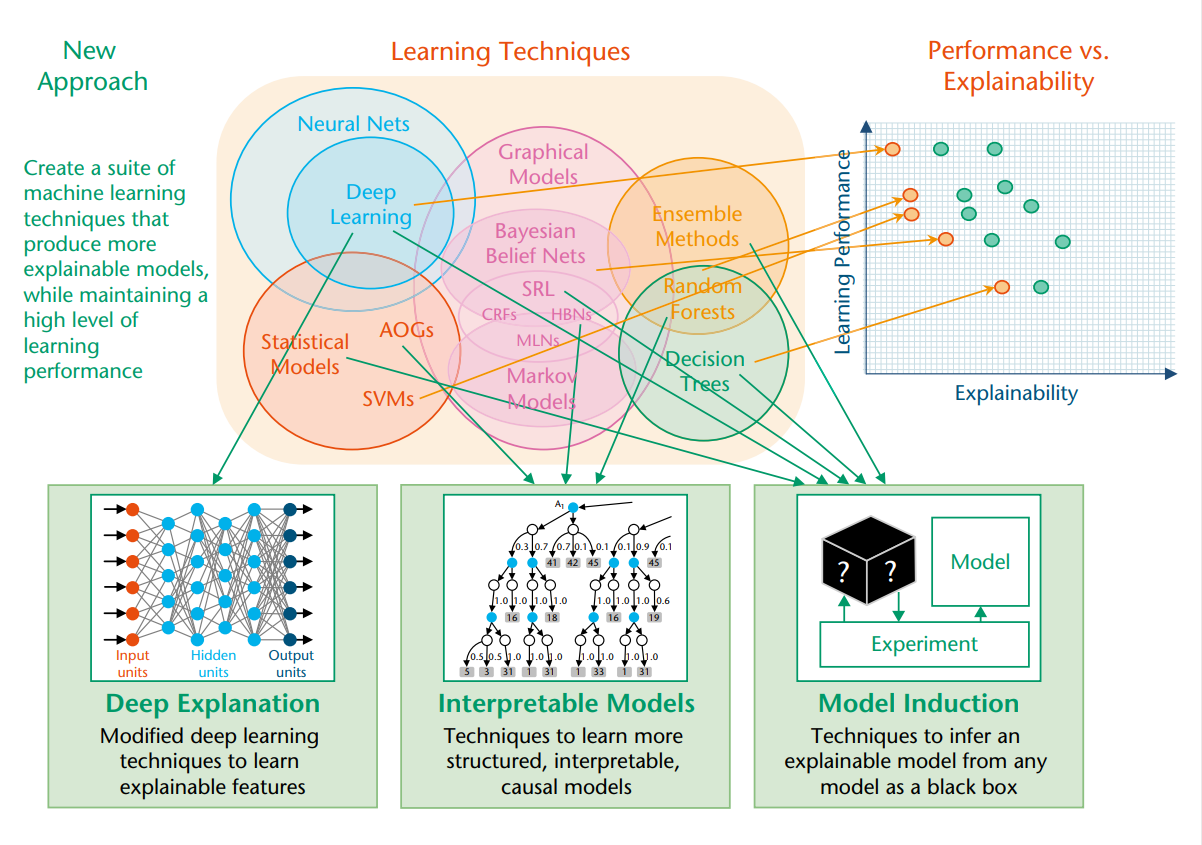
\includegraphics[width=0.8\textwidth]{images/darpa_xai_strategies.png}
\caption{Strategies for developing explainable models showing the relationship between learning techniques, performance vs explainability trade-offs, and three main XAI approaches: Deep Explanation, Interpretable Models, and Model Induction.}
\label{fig:darpa_xai_strategies}
\end{figure}

The DARPA XAI program identifies three primary strategies for developing explainable models, as illustrated in Figure \ref{fig:darpa_xai_strategies}. These approaches represent different methodological directions for addressing the fundamental trade-off between model performance and explainability.

\subsection{Defining Explainability vs. Interpretability}

While interpretability and explainability are frequently used interchangeably within the Machine Learning community, subtle yet important distinctions exist between these concepts. Biran and Cotton's \cite{Biran2017ExplanationAJ} define interpretability as "the degree to which an observer can understand the cause of a decision". From a Machine Learning perspective, interpretability encompasses understanding how decisions or predictions are generated by ML algorithms through logical reasoning. Explainability, conversely, relates more closely to the internal operational mechanisms of black-box models \cite{alicioglu2021survey}.

XAI aims to reveal the internal functioning of black-box models and the underlying reasoning of their decisions, through various methodological approaches. While domain experts inexperienced in Machine Learning typically seek understanding through reasoning and cause-effect relationships for specific decisions, Machine Learning scientists focus on the internal operational mechanisms of models, attempting to understand how individual components contribute to particular predictions \cite{alicioglu2021survey}.

\subsection{XAI Taxonomy and Approaches}

Despite the growing importance of XAI, no standardized consensus exists regarding its precise definition \cite{emmert2020explainable,adadi2018peeking,das2020opportunities}. This definitional diversity stems from varying domain-specific applications, use-case scenarios, and research objectives \cite{alicioglu2021survey}.

% Source: A survey of visual analytics for Explainable Artificial Intelligence methods.pdf, Page 4  
\begin{table}
    \centering
    \caption{Classification of the most popular XAI techniques in explaining neural networks.}
    \label{tab:xai_classification}
    \begin{adjustbox}{width=\textwidth,center}
        \begin{tabular}{|c|cc|cc|cc|}
        
        \hline
        \multirow{2}{*}{\textbf{XAI method}} & 
        \multicolumn{2}{c|}{\textbf{Explanation level}} & 
        \multicolumn{2}{c|}{\textbf{Implementation level}} & 
        \multicolumn{2}{c|}{\textbf{Model dependency}} \\
        \cline{2-7}
                                                                                     & Global     & Local      & Intrinsic  & Post hoc   & Agnostic   & Specific \\
        \hline
        ANCHORS \cite{10.5555/3504035.3504222}                                       &            & \checkmark &            & \checkmark & \checkmark &            \\
        LIME \cite{ribeiro2016should}                                                & \checkmark & \checkmark &            & \checkmark & \checkmark &            \\
        SHAP \cite{lundberg2017unified}                                              &            & \checkmark &            & \checkmark & \checkmark &            \\
        LRP \cite{Bach2015OnPE}                                                      & \checkmark & \checkmark &            & \checkmark & \checkmark &            \\
        Grad-CAM \cite{Selvaraju_2019}                                               &            & \checkmark &            & \checkmark & \checkmark &            \\
        Saliency Maps \cite{simonyan2014deepinsideconvolutionalnetworks}             &            & \checkmark &            & \checkmark & \checkmark &            \\
        Integrated Gradients \cite{sundararajan2017axiomaticattributiondeepnetworks} &            & \checkmark &            & \checkmark & \checkmark &            \\
        DeepLIFT \cite{shrikumar2019learningimportantfeaturespropagating}            &            & \checkmark &            & \checkmark & \checkmark &            \\
        Bayesian Rule Lists \cite{Letham_2015}                                       & \checkmark &            & \checkmark &            &            & \checkmark \\
        Distillation \cite{10.1145/3278721.3278725}                                  & \checkmark &            &            & \checkmark & \checkmark &            \\
        GAM \cite{10.1145/2783258.2788613}                                           & \checkmark &            & \checkmark &            &            & \checkmark \\
        Mean Decrease Impurity \cite{breiman2002manual}                              & \checkmark & \checkmark & \checkmark &            &            & \checkmark \\
        CAM \cite{7780688}                                                           &            & \checkmark &            & \checkmark & \checkmark &            \\
        \hline
        
    \end{tabular}
    \end{adjustbox}
\end{table}


XAI methods can be categorized along three primary dimensions, as shown in Table \ref{tab:xai_classification}:

\textbf{Explanation Level:} This dimension distinguishes between \textit{global explanations}, which focus on the overall model behavior and decision-making mechanisms, and \textit{local explanations}, which untangle model decisions for individual instances or subpopulations \cite{alicioglu2021survey}. Global methods such as Bayesian Rule Lists (BRL) \cite{Letham_2015}, Generalized Additive Models (GAM), and model distillation techniques provide comprehensive model-wide insights. In contrast, local methods including Local Interpretable Model-Agnostic Explanations (LIME) \cite{ribeiro2016should}, SHapley Additive exPlanations (SHAP) \cite{lundberg2017unified}, Gradient-weighted Class Activation Mapping (Grad-CAM), and Deep Learning Important FeaTures (DeepLIFT) focus on instance-specific explanations.

\textbf{Implementation Level:} This categorization distinguishes between \textit{intrinsic} and \textit{post-hoc} explanations \cite{alicioglu2021survey}. Intrinsic explanations, such as Bayesian Rule Lists and Mean Decrease Impurity (MDI), are provided directly by the model through parameters, decision trees, or rule structures. Post-hoc explanations, on the other side, analyze pre-trained models to reveal internal functioning and decision mechanisms after the training process completion.

\textbf{Model Dependency:} Methods are classified as either \textit{model-agnostic} (applicable across different model types) or \textit{model-specific} (tailored to particular architectures) \cite{bodria2023benchmarking}.

\subsection{Core Challenges and Goals}

The development of eXplainable AI is driven by interconnected objectives that address both technical and human-centered concerns. At its foundation, XAI tires to increase \textbf{trust and transparency} in AI systems by providing clear insights into their decision-making processes. This transparency is particularly crucial in high-stakes domains such as healthcare, finance, and criminal justice, where algorithmic decisions can have profound consequences on individuals' lives and where accountability is not merely desirable but legally and ethically necessary.

Beyond increasing trust, XAI must fill the gap between internal mechanisms of complex machine learning models and human comprehension. Effective explanations need to be tailored to diverse audiences, accommodating the needs of technical experts who may require algorithmic insights as well as non-specialist end-users who benefit from intuitive, accessible descriptions. This challenge of achieving multi-level interpretability represents one of the field's most persistent obstacles, as explanation systems must balance technical accuracy with cognitive accessibility.

Moreover, XAI should deliver \textbf{actionable insights} that empower users to understand not only \textit{what} decision a model has reached, but \textit{why} it arrived at that particular conclusion. This deeper level of understanding enables informed decision-making, allowing users to appropriately trust, question, or override model predictions based on contextual factors that may not be captured in the training data. Such actionability extends beyond passive understanding to active engagement with AI systems, transforming users from mere consumers of predictions into evaluators of algorithmic reasoning.

From a technical perspective, XAI techniques serve a role in \textbf{models improvement}. By revealing the internal logic of models, explanation methods facilitate debugging, bias detection, and performance enhancement, exposing potential weaknesses, unexpected behaviours, or antagonistic correlations that might otherwise remain hidden. This diagnostic capability is essential for developing robust and fair AI systems that can be safely deployed in real-world applications.

The field continues to evolve rapidly, with ongoing research addressing fundamental challenges including explanation consistency, computational efficiency, and the development of standardized evaluation metrics for explanation quality \cite{bodria2023benchmarking}. As XAI matures, the integration of visual analytics techniques with sophisticated explanation methods promises to deliver more effective human-AI collaborative systems.

\subsection{Most common XAI Algorithm}

The field of eXplainable Artificial Intelligence methods has been largely defined by two groundbreaking approaches: LIME (Local Interpretable Model-Agnostic Explanations) and SHAP (SHapley Additive exPlanations). These techniques target the same fundamental problem, how do we understand what a complex model is thinking when it makes a specific prediction? These methods represent distinct approaches to the task of instance level explainability, each proposing unique mechanisms that have influenced the development of subsequent explanation techniques.

\subsubsection{LIME: Local Interpretable Model-Agnostic Explanations}

LIME, introduced by Ribeiro et al.\cite{ribeiro2016should}, operates on the principle that complex models can be explained locally through simple, interpretable surrogate models \cite{ribeiro2016should, bodria2023benchmarking}. The core mechanism of LIME involves generating a synthetic neighborhood, around the instance to be explained, through random perturbation, where samples are drawn both in the vicinity of the target instance and further away\cite{ribeiro2016should, bodria2023benchmarking}. This neighborhood generation exploits a proximity measure $\pi_x(z)$, between an instance $z$ to the explained instance $x$, to capture locality around $x$, ensuring that nearby instances receive greater emphasis in the explanation process.

The method samples instances around the target instance $x$ by drawing nonzero elements at random, creating a perturbed dataset $\{z \in \mathbb{R}^d\}$ that is subsequently labeled by the black-box model $b(z)$ \cite{ribeiro2016should, bodria2023benchmarking}. LIME then trains a sparse linear model on these perturbed samples, with the explanation consisting of feature importance weights from this local linear approximation \cite{ribeiro2016should, guidotti2022stable}.

\textbf{Visual Affordances:} LIME's explanations are typically presented through \textit{bar charts} that display feature importance values, clearly distinguishing between positive and negative contributions to the prediction \cite{alicioglu2021survey, ribeiro2016should}. These visualizations allow end-users to easily observe both supportive and contradictory feature influences, making the local decision boundary accessible through intuitive graphical representations \cite{alicioglu2021survey}. One can observe two examples of LIME's explanations in Figure \ref{fig:LimeExpExamp}.

\begin{figure}[htbp]
    \centering
    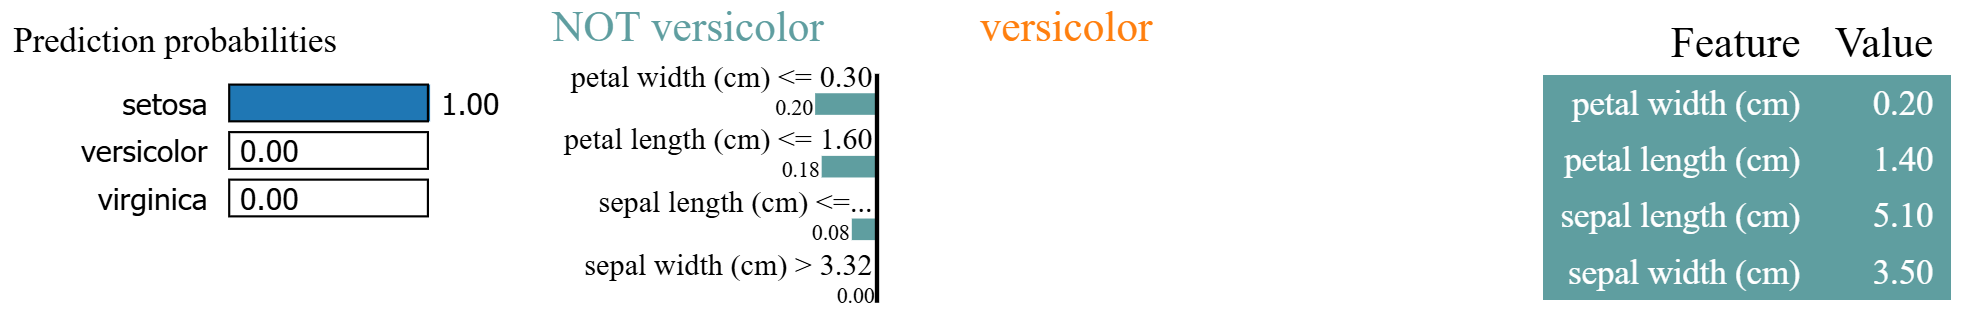
\includegraphics[width=1\textwidth]{images/limeexplain1.png}
    
    \vspace{0.5cm} 
    
    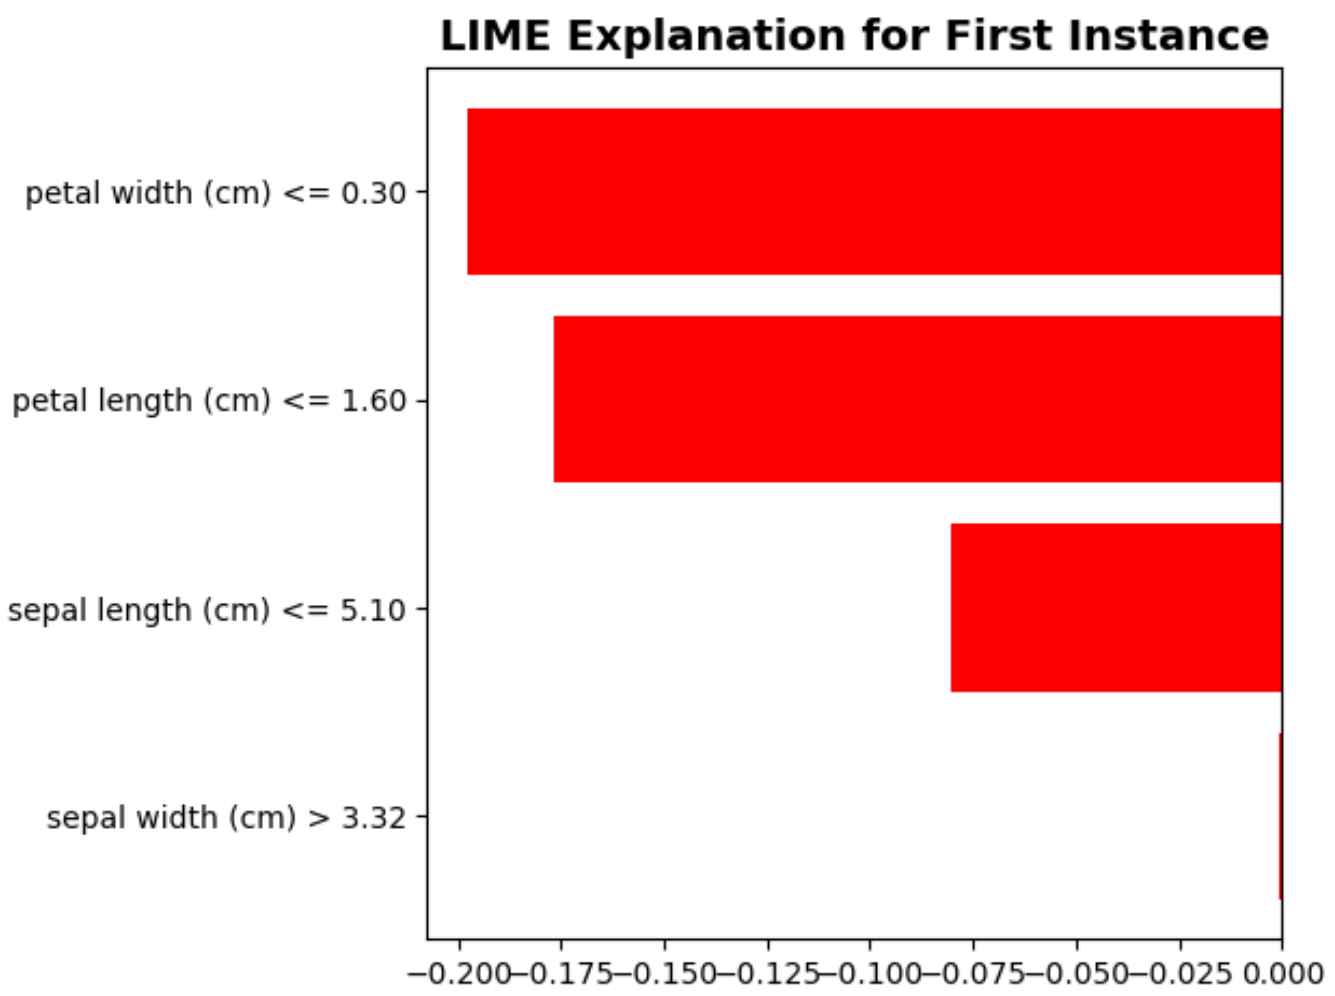
\includegraphics[width=0.6\textwidth]{images/limeexplain2.png}
    \caption{Examples of LIME explanations}
    \label{fig:LimeExpExamp}
\end{figure}

\subsubsection{SHAP: SHapley Additive exPlanations}

SHAP, developed by Lundberg et. al \cite{lundberg2017unified}, takes a fundamentally different approach rooted in cooperative game theory. The method computes feature importance through Shapley values, treating features as players in a cooperative game and calculating their marginal contributions to the prediction outcome \cite{alicioglu2021survey}. SHAP explanations are \textit{additive feature attributions} that satisfy the mathematical formulation: $g(z') = \phi_0 + \sum_{i=1}^{M} \phi_i z'_i$, where $z' \in \{0,1\}^M$, $\phi_i \in \mathbb{R}$ represent effects assigned to each feature, and $M$ denotes the number of simplified input features \cite{lundberg2017unified, bodria2023benchmarking}.

The method maintains three crucial properties: (i) \textit{local accuracy}, ensuring $f(x) = g(x') = \phi_0 + \sum^M_{i=1}\phi_ix'_i$, meaning that the explanation model $g(x')$ matches the original model $f(x)$ when $x=h_x(x')$; (ii) \textit{missingness}, where features with $x_i = 0$ have no attributed impact; and (iii) \textit{consistency}, guaranteeing that increased marginal feature contributions result in increased SHAP values \cite{lundberg2017unified, bodria2023benchmarking}. SHAP provides both local explanations for individual instances and global insights through collective SHAP value analysis \cite{bodria2023benchmarking}.

\textbf{Visual Affordances:} SHAP offers diverse visualization techniques including \textit{bar plots} that display feature importance rankings, \textit{beeswarm plots} that combine feature importance with feature effects for each sample, \textit{decision plots} showing the cumulative effect of features on individual predictions, \textit{force plots} that show how each feature pushes the prediction away from a base value, \textit{heatmap plots} for visualizing feature effects across multiple samples, \textit{image plots} designed specifically for computer vision models to highlight relevant pixels, \textit{scatter plots} that reveal the relationship between feature values and their SHAP values, \textit{text plots} for natural language processing models to highlight important words or tokens, \textit{violin summary plots} that show the distribution of SHAP values for each feature, and \textit{waterfall plots} displaying sequential feature contributions that show how each feature pushes the prediction away from a base value \cite{shapDocumentationOnline}. Some of those visualizations, on the same instance of the iris dataset as the one used in LIME's Figures \ref{fig:LimeExpExamp}, can be observed in Figure \ref{fig:shapAllViz}

\begin{figure}[htbp]
    \centering
    
    \begin{subfigure}[c]{0.385\textwidth}
        \centering
        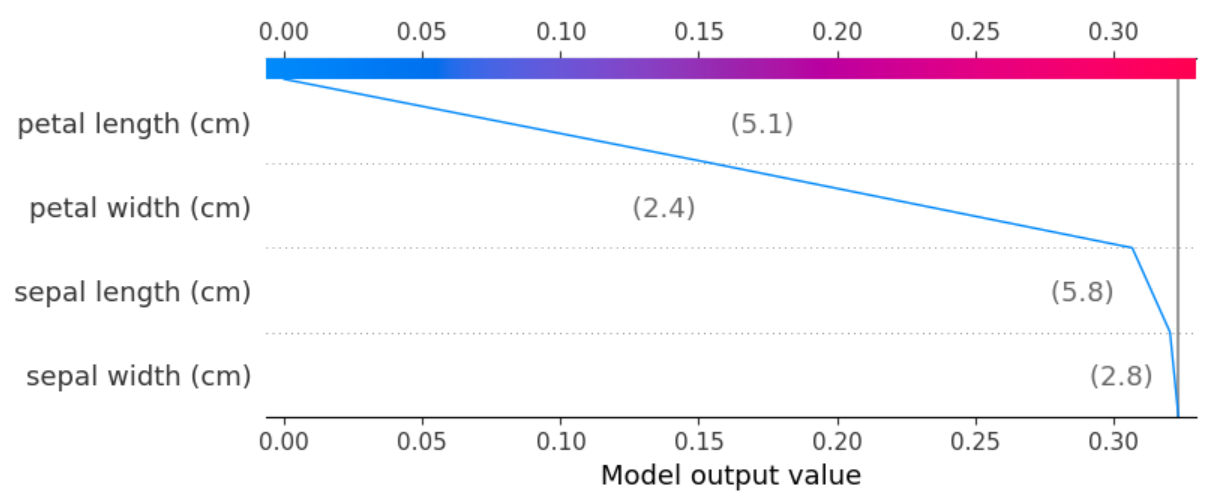
\includegraphics[width=\textwidth]{images/shapDecisionPlot.png}
        \caption{SHAP decision plot showing the cumulative impact of features on model prediction}
        \label{fig:shap_decision}
    \end{subfigure}
    \hfill
    \begin{subfigure}[c]{0.385\textwidth}
        \centering
        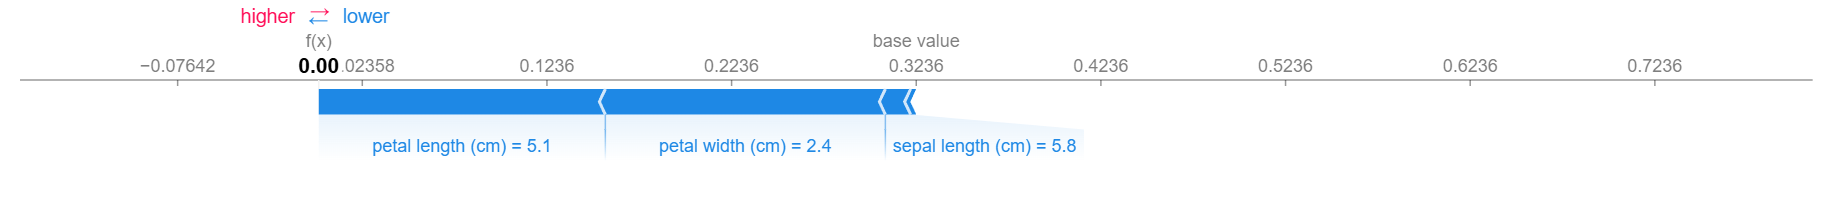
\includegraphics[width=\textwidth]{images/shapForcePlot.png}
        \caption{SHAP force plot displaying individual prediction explanation with features contributing positively (red) and negatively (blue) to push the prediction above or below the base value}
        \label{fig:shap_force}
    \end{subfigure}
    
    \vspace{0.5cm}
    
    \begin{subfigure}[c]{0.385\textwidth}
        \centering
        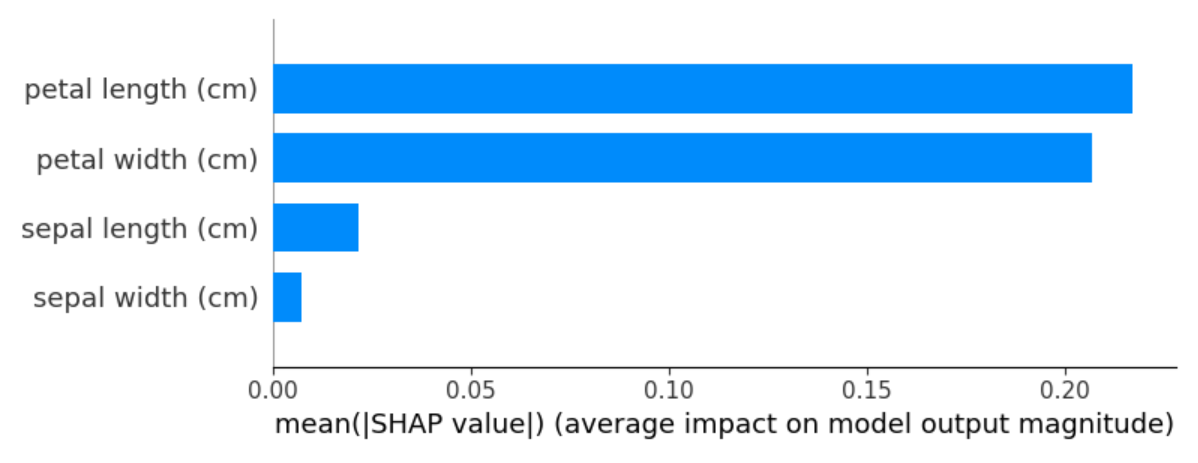
\includegraphics[width=\textwidth]{images/shapSummaryPlot.png}
        \caption{SHAP summary plot showing feature importance and impact distribution}
        \label{fig:shap_summary}
    \end{subfigure}
    \hfill
    \begin{subfigure}[c]{0.385\textwidth}
        \centering
        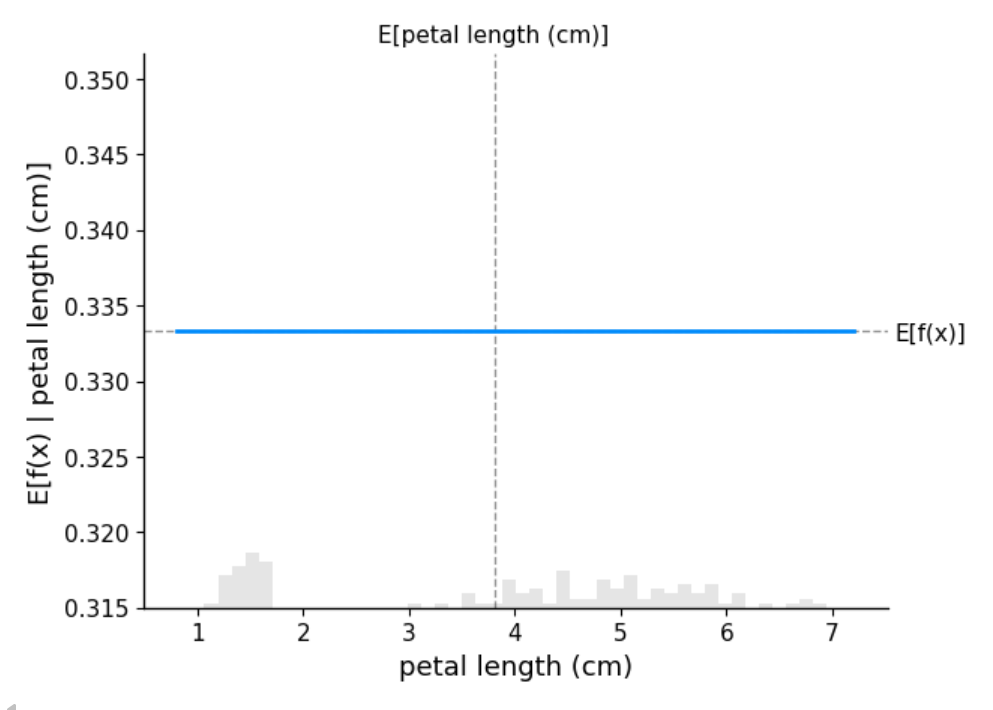
\includegraphics[width=\textwidth]{images/shapPartialDependencePlot.png}
        \caption{Partial dependence plot showing model output vs feature values}
        \label{fig:shap_dependence}
    \end{subfigure}
    
    \vspace{0.5cm}
    
    \begin{subfigure}[c]{0.385\textwidth}
        \centering
        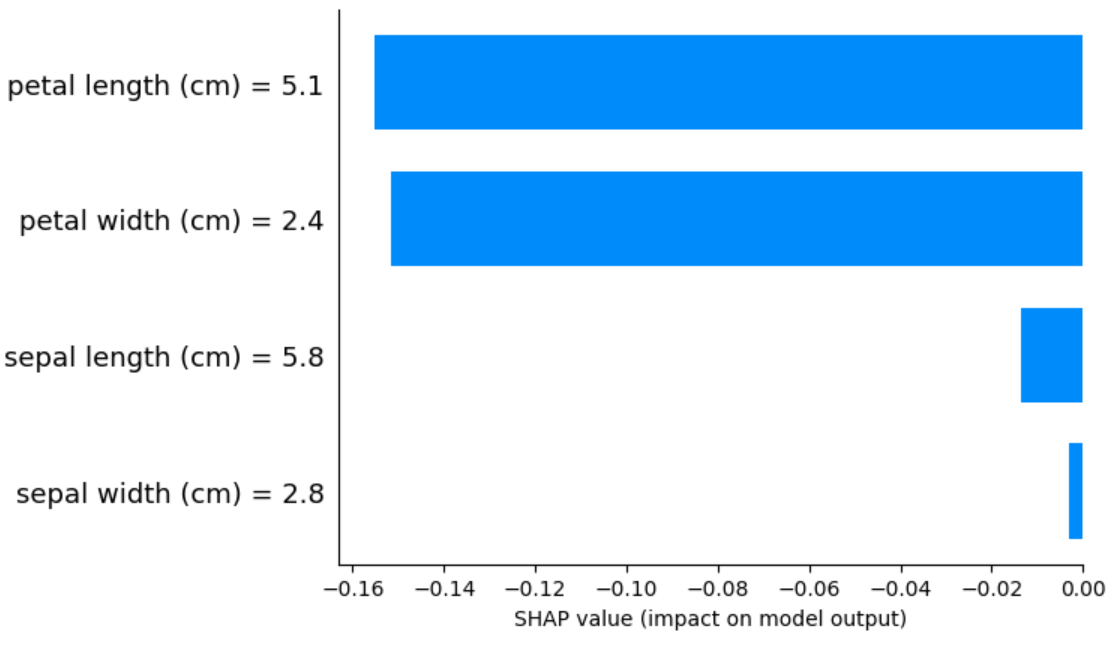
\includegraphics[width=\textwidth]{images/shapBarPlot.png}
        \caption{SHAP bar plot showing individual feature contributions}
        \label{fig:shap_bar}
    \end{subfigure}
    \hfill
    \begin{subfigure}[c]{0.385\textwidth}
        \centering
        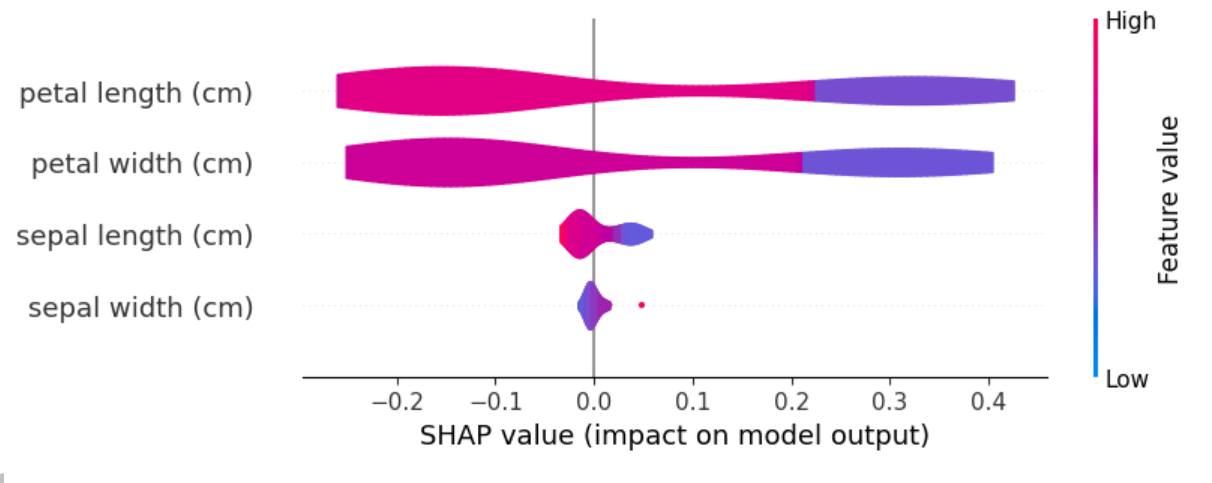
\includegraphics[width=\textwidth]{images/shapViolinPlot.png}
        \caption{SHAP violin plot showing distribution and impact of feature contributions on model predictions}
        \label{fig:shap_violin}
    \end{subfigure}
    
    \caption{Some of SHAP' visualizations showing different aspects of model interpretability on the iris dataset instance 'sepal length (cm)': 5.8, 'sepal width (cm)': 2.8, 'petal length (cm)': 5.1, 'petal width (cm)': 2.4.}
    \label{fig:shapAllViz}
\end{figure}

% Source: Opportunities and Challenges in Explainable Artificial Intelligence XAI A Survey.pdf, Page 19
\begin{figure}[ht]
\centering
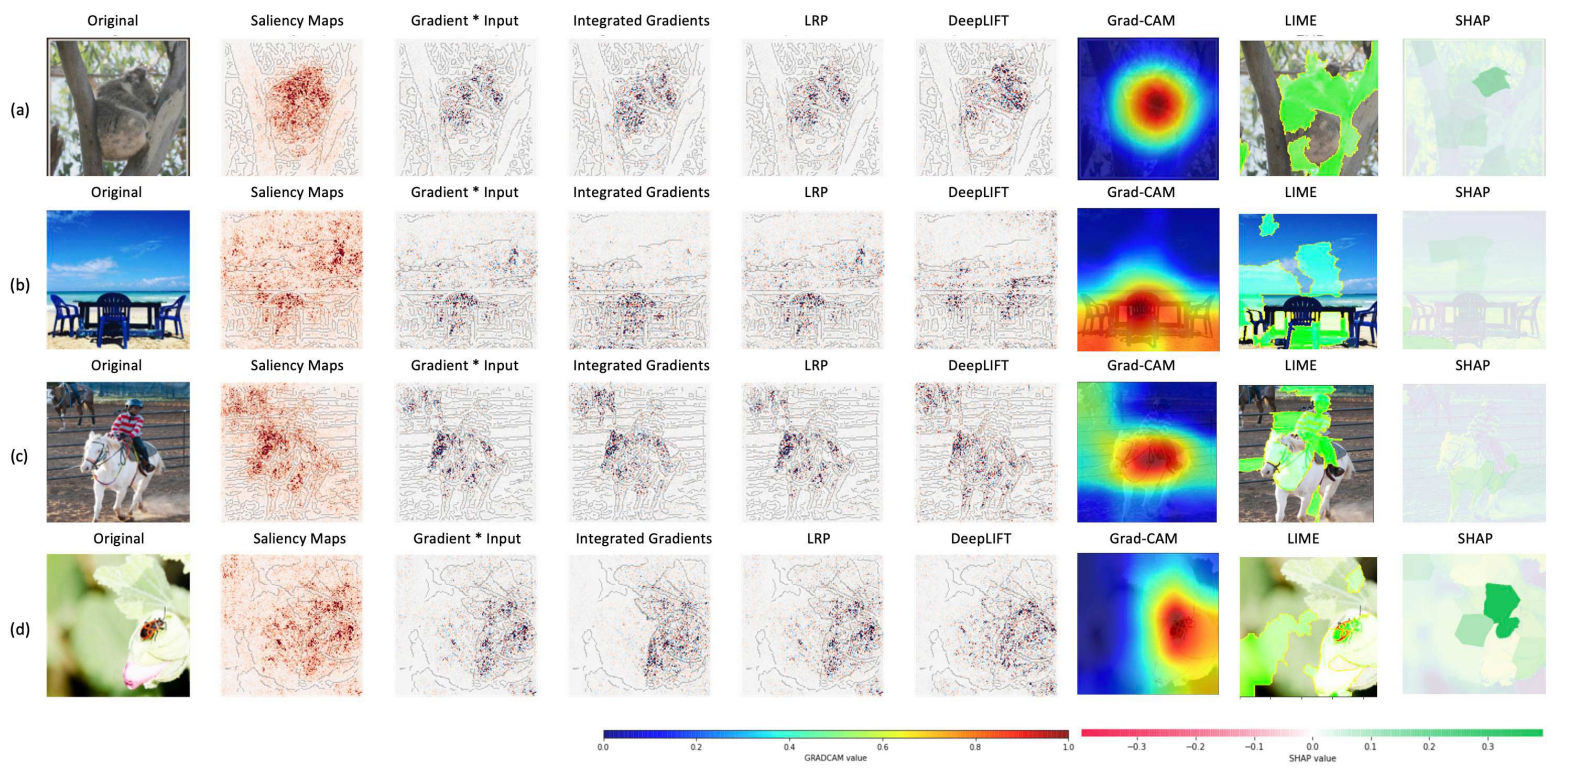
\includegraphics[width=\textwidth]{images/xai_methods_comparison.png}
\caption{Evaluation different gradient-based and perturbation-based techniques in this figure. LIME and SHAP uses segmented superpixels to understand feature importance, while gradient based saliency maps, Integrated Gradients, LRP, DeepLIFT, and Grad-CAM use backpropagation based feature importance
in a pixel level \cite{das2020opportunities}.}
\label{fig:xai_methods_comparison}
\end{figure}

\subsubsection{Comparative Analysis of LIME and SHAP}

The comparison between LIME and SHAP reveals distinct trade-offs across multiple evaluation dimensions, as demonstrated in Figure \ref{fig:xai_methods_comparison} which shows how both methods perform on real image classification tasks compared to gradient-based approaches:

\textbf{Fidelity:} As shown in Table \ref{tab:fidelity_faithfulness}, empirical evaluations demonstrate that LIME generally exhibits higher fidelity values compared to SHAP, particularly on adult dataset classifications \cite{bodria2023benchmarking}. LIME achieves fidelity scores above 90\% across most model types, while SHAP shows notably lower performance on ensemble models such as CatBoost, with values dropping to 0.777 for CatBoost on adult data and 0.670 on German credit data \cite{bodria2023benchmarking}. This suggests that LIME's linear surrogate models more accurately approximate local black-box behavior in many scenarios.

\begin{table}[ht]
    \centering
    \caption{Comparison of the fidelity and the faithfulness metrics of different explanation methods from \cite{bodria2023benchmarking}. Bold values indicate the best results. For every evaluation, the mean and the standard deviation over a subset of 50 test set records is reported}
    \label{tab:fidelity_faithfulness}
    \begin{adjustbox}{width=\textwidth,center}
    \begin{tabular}{llcccccc}
        \hline
        \textbf{Dataset} & \textbf{Black-Box} & \multicolumn{4}{c}{\textbf{Fidelity}} & \multicolumn{2}{c}{\textbf{Faithfulness}} \\
        \cline{3-6} \cline{7-8}
         &  & LIME & SHAP & ANCHOR & LORE & LIME & SHAP \\
        \hline
        adult  & LG  & 0.979 & 0.613 & \textbf{0.989} & 0.984 & 0.099 (0.30) & \textbf{0.38} (0.37) \\
               & XGB & 0.977 & 0.877 & 0.978 & \textbf{0.982} & 0.030 (0.32) & \textbf{0.36} (0.49) \\
               & CAT & 0.960 & 0.777 & 0.988 & \textbf{0.989} & 0.077 (0.32) & \textbf{0.44} (0.37) \\
        \hline
        german & LG  & \textbf{0.984} & 0.910 & 0.730 & 0.983 & \textbf{0.23 }(0.60)  & 0.19 (0.63) \\
               & XGB & \textbf{0.999} & 0.821 & 0.802 & 0.982 & 0.16 (0.26)  & \textbf{0.44 }(0.21) \\
               & CAT & 0.979 & 0.670 & 0.620 & \textbf{0.981} & 0.34 (0.33)  & \textbf{0.43 }(0.32) \\
        \hline
    \end{tabular}
    \end{adjustbox}
\end{table}

\textbf{Faithfulness:} Conversely, SHAP demonstrates superior faithfulness compared to LIME across experimental datasets \cite{bodria2023benchmarking}. For the German credit dataset, SHAP achieves faithfulness values of 0.19-0.44, while LIME scores range from 0.16-0.34. On the adult dataset, SHAP consistently outperforms LIME, achieving 0.44 faithfulness with CatBoost compared to LIME's 0.077 \cite{bodria2023benchmarking}. This indicates that SHAP explanations more accurately reflect the true feature influences despite lower fidelity scores.

\textbf{Interpretability:} Both methods offer distinct interpretability advantages. LIME's feature importance vectors are straightforward for domain experts who understand feature meanings, but may prove challenging for non-technical users when importance values are complex \cite{lundberg2017unified, bodria2023benchmarking}. SHAP's mathematical foundation provides theoretical guarantees but introduces complexity in understanding how base values, output values, and feature importance arrays combine to form explanations \cite{bodria2023benchmarking}.

\textbf{Consistency:} Both methods exhibit poor consistency performance, with neither achieving remarkable consistency according to established metrics \cite{bodria2023benchmarking}. This inconsistency represents a shared weakness across many explanation methods, highlighting the need for more robust explanation generation procedures.

    
    \section{Visualizations for XAI}\label{sec:Visualizations for XAI}
        The following section reviews the literature and techniques that inform the development of the thesis visualization system. Since local explainability methods mostly rely on the same principle of generating a synthetic neighborhood and the training of a surrogate model, this review is structured to address the key components of our interactive explanation system. We begin by examining dimensionality reduction techniques that enable visual exploration of high-dimensional synthetic data in a reduced dimensional space. Subsequently, we explore the literature on decision tree visualization, as decision trees constitute the primary surrogate model employed for rule extraction. Finally, we survey existing visual tools and interactive techniques in eXplainable Artificial Intelligence.
        \subsection{Dimensionality Reduction Techniques}
        In the context of eXplainable Artificial Intelligence
% , particularly for systems like $\text{LORE}_{sa}$, 
the visualization of high-dimensional data is of high relevance. When 
% $\text{LORE}_{sa}$ 
an explainability method
generates synthetic neighborhoods around the instance to be explained, the generated neighborhoods typically exist in a high-dimensional feature space that is difficult to interpret and visualize directly. Dimensionality reduction techniques serve as essential tools for projecting these multi-dimensional datasets into two or three-dimensional representations that enable human comprehension and interactive exploration \cite{yang2021dimensionality}.

The primary objective of dimensionality reduction in visual XAI is to preserve meaningful relationships and structures present in the original high-dimensional space while facilitating intuitive visual interpretation. 
% For $\text{LORE}_{sa}$'s, 
This capability is particularly crucial as it allows users to spatially explore the synthetic neighborhood and understand the distribution of generated instances. The choice of dimensionality reduction technique significantly impacts the quality of explanations. Different methods preserve distinct aspects of the data structure, while some excel at maintaining local neighborhoods, others are very good at preserving global relationships \cite{becht2019evaluation}.

% This challenge becomes more pronounced when dealing with the diverse nature of synthetic neighborhoods generated by $\text{LORE}_{sa}$'s genetic algorithms.
The effectiveness of different dimensionality reduction methods varies depending on the characteristics of the dataset, the size of the synthetic neighborhood, and the specific visual analytics requirements of the explanation task \cite{wang2021understanding}. The evaluation of dimensionality reduction techniques requires careful consideration of both local and global structure preservation criteria.

The following subsections examine four dimensionality reduction techniques. Each technique exhibits distinct characteristics in preserving data structure. We begin with \textbf{Principal Component Analysis (PCA)}, the most widely adopted linear method known for its computational efficiency and interpretability of component meanings. This is followed by \textbf{Multidimensional Scaling (MDS)}, a classical approach that focuses on preserving pairwise distances between data points. Subsequently, we explore \textbf{t-distributed Stochastic Neighbor Embedding (t-SNE)}, known for its effectiveness in revealing local cluster structures, though with limitations in global structure preservation. Finally, \textbf{Uniform Manifold Approximation and Projection (UMAP)}, which has shown superior performance in preserving both local and global structure while maintaining computational efficiency for large-scale synthetic neighborhoods.

The following subsections provide a detailed examination of each technique, followed by a comparative analysis that evaluates their relative performance across key criteria, including structure preservation, computational efficiency, and visual quality for neighborhood exploration. 

\subsubsection{PCA (Principal Component Analysis)}

Principal Component Analysis (PCA) represents one of the, if not the most, widely adopted linear dimensionality reduction technique in data analysis, with historical foundations dating back to the pioneering work of Pearson (1901) and Hotelling (1933) \cite{sewell2008pca}. As a fundamental method in multivariate statistics, PCA aims to reduce the dimensionality of datasets while preserving as much relevant information as possible through variance maximization \cite{sewell2008pca}.

% Source: Principal Component Analysis: A Natural Approach to Data Exploration, Page 70:3
\begin{figure}[htbp]
    \centering
    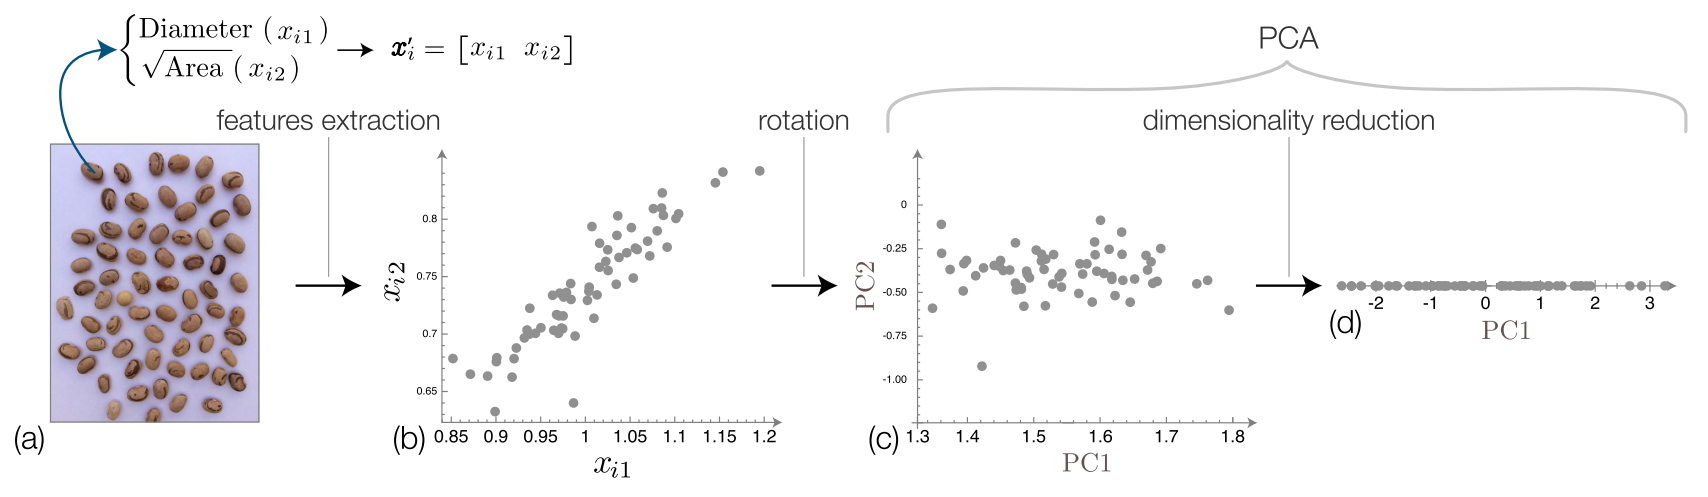
\includegraphics[width=1.0\textwidth]{images/PCA1.png}
    \caption{Illustration of the PCA process using real-world bean data. bean (a) is characterized in terms of two features: diameter xi1 and square root of area xi2. Though these two features are intrinsically related in a direct fashion,
bean shape variations induce a dispersion of the objects when mapped into the features space (b). PCA allows the identification of the orientation of maximum data dispersion (c). As the dispersion in the resulting
second axis is relatively small, this axis can be eventually disregarded (d).}
    \label{fig:pca_process}
\end{figure}

The theoretical foundation of PCA rests on the principles of linear transformation, where the algorithm transforms the data to a new coordinate system such that the new variables (principal components) are linear functions of the original variables, are not correlated, and are ordered by the amount of variance that they explain \cite{sewell2008pca}. The transformation operates as a rotation of the coordinate system that aligns the axes with the directions of maximum data variation \cite{gewers2021pca}, as illustrated in Figure~\ref{fig:pca_process}. This process can be expressed in matrix form as $Y = XW$, where $X$ represents the original data matrix, $W$ is the transformation matrix composed of eigenvectors, and $Y$ contains the principal component scores.

The algorithm's core mechanism involves computing the covariance matrix of the dataset, followed by eigenvalue decomposition to obtain eigenvectors and eigenvalues sorted in decreasing order \cite{sewell2008pca}. Each eigenvector defines the direction of a principal component, while the corresponding eigenvalue quantifies the amount of variance explained along that direction \cite{gewers2021pca}. An essential property of PCA is that the total data variance is preserved under the transformation: $\sum_{j=1}^{n} \sigma^2_{x_j} = \sum_{j=1}^{n} \sigma^2_{y_j}$, meaning the variance along each principal component equals the corresponding eigenvalue of the covariance matrix \cite{gewers2021pca}.

A distinctive characteristic of PCA is its ability to provide direct interpretability through loadings analysis. The transformation matrix $W$ contains eigenvectors that indicate how the original features contribute to each principal component, allowing users to understand which variables drive the main sources of variation in the data \cite{gewers2021pca}. 
PCA demonstrates particular effectiveness in scenarios involving correlated features, where the method can achieve substantial dimensionality reduction while retaining most of the original variance.
PCA's deterministic nature 
provides stability that is particularly valuable in interactive applications where consistent visualizations are required \cite{gewers2021pca}.

Particularly significant for 
eXplainable AI
% $\text{LORE}_{sa}$ 
applications is PCA's unique capability to preserve the structure of decision boundaries generated by the local surrogate models. Since PCA applies a linear transformation, the decision boundaries created by
% $\text{LORE}_{sa}$'s 
linear surrogate model maintain their essential geometric properties when projected into the two-dimensional visualization space. This preservation enables users to observe how the surrogate model rules translate into spatial regions within the spatial neighborhood analysis plot visualization, providing a direct correspondence between the rule-based explanations and the visual representation of the synthetic neighborhood. This characteristic distinguishes PCA from other dimensionality reduction techniques that may significantly distort or obscure the decision boundaries due to their nonlinear transformations.

However, PCA's linear assumption may limit its effectiveness for datasets with complex nonlinear structures. The algorithm's focus on variance maximization means that directions with high variance are prioritized regardless of their relevance for specific analytical tasks \cite{gewers2021pca}. 

\subsubsection{MDS (Multidimensional Scaling)}

Multidimensional Scaling (MDS) has theoretical origins tracing back to the pioneering work of Torgerson (1952) \cite{torgerson1952mds} in developing systematic methods for scaling multidimensional psychological and perceptual data. 

The core principle underlying MDS involves the preservation of pairwise distances between data points across different dimensional representations \cite{torgerson1952mds, mcinnes2020umap}. The algorithm operates by constructing a low-dimensional embedding where the Euclidean distances between points in the reduced space approximate as closely as possible the original distances (or dissimilarities) measured in the high-dimensional space. This distance-preserving objective distinguishes MDS from techniques that focus primarily on local neighborhood relationships or topological structures.

Classical MDS, also known as Principal \textbf{Coordinate} Analysis, employs a three-step procedure as originally formulated by Torgerson \cite{torgerson1952mds}.
The first step involves obtaining a scale of comparative distances between all pairs of stimuli (any set of objects, items, concepts, or entities in study), analogous to paired comparison methods but applied to distance relationships rather than direct stimulus comparisons. The second step requires estimating an additive constant to convert these comparative distances into absolute distances, addressing the inherent indeterminacy in the zero point of the distance scale. The third step determines the dimensionality of the space necessary to account for these absolute distances and computes the projections of data points onto the axes of this space.

MDS demonstrates particular strength in preserving global structure and long-range distance relationships within data \cite{mcinnes2020umap}. The algorithm's explicit focus on maintaining the full distance matrix makes it especially suitable for applications where all scales of structure are equally important, and where the preservation of metric relationships takes precedence over local neighborhood fidelity. This global perspective allows MDS to maintain meaningful relative positions between widely separated clusters or groups within the data.

The technique has robust theoretical properties from its foundation in classical metric geometry. Since MDS minimizes the sum of squared errors between original and embedded distances, it provides a principled approach to dimensionality reduction with well-understood optimality properties. The linear nature of classical MDS ensures deterministic results and computational stability, avoiding the convergence issues that can affect iterative nonlinear methods.

However, MDS faces several inherent limitations that constrain its effectiveness in specific visualization contexts. The algorithm's emphasis on preserving large pairwise distances can come at the expense of local neighborhood structure, potentially causing nearby points in the original space to appear more separated in the reduced dimensional representation than would be ideal for cluster identification \cite{maaten2008tsne}. This focus on global distance preservation means that MDS may not effectively capture local manifold structure or fine-grained clustering patterns that are crucial for understanding local decision boundaries in eXplainable AI applications.

Empirical evaluations on transcriptomic datasets reveal that MDS exhibits moderate performance in neighborhood preservation, 
indicating that local neighborhood relationships are less well preserved compared to methods specifically designed for local structure preservation \cite{yang2021dimensionality}. 
% In terms of computational efficiency, MDS shows the slowest runtime performance among the major dimensionality reduction techniques, particularly for larger datasets.

The algorithm's linear transformation approach means that MDS may struggle with datasets containing complex nonlinear manifold structures. While this linearity provides interpretability advantages similar to PCA, it can result in poor representations for data that lies on curved or twisted manifolds where Euclidean distances in the original space do not accurately reflect the intrinsic geometric relationships.

Despite these limitations, MDS offers several advantages for specific analytical contexts. The method's deterministic nature ensures reproducible results, which can be valuable for comparative analyses and scientific reporting. The explicit distance preservation objective makes MDS particularly suitable for applications where the maintenance of quantitative distance relationships is more important than the visual separation of clusters or local neighborhoods.

For 
% $\text{LORE}_{sa}$ 
synthetic neighborhoods visualization applications, MDS presents a mixed proposition. While the algorithm's distance preservation properties might maintain some aspects of the original synthetic neighborhood structure, its tendency to emphasize global relationships over local patterns may not optimally support the identification of 
local explanation regions that are central to 
% $\text{LORE}_{sa}$'s
eXplainable AI systems
interpretability objectives. 
Modern variants of MDS, including metric and non-metric forms, have been developed to address some of these limitations, but the classical formulation remains the most commonly implemented 
approach. 

\subsubsection{t-SNE (t-distributed Stochastic Neighbor Embedding)}

t-distributed Stochastic Neighbor Embedding (t-SNE) represents a nonlinear dimensionality reduction technique designed for data visualization \cite{maaten2008tsne}. Developed as an improvement over Stochastic Neighbor Embedding (SNE), t-SNE addresses fundamental challenges in high-dimensional data visualization by employing probabilistic modeling of pairwise similarities and takes advantage of heavy-tailed distributions to overcome the crowding problem in dimension reduction \cite{maaten2008tsne}.

\begin{figure}
    \centering
    \begin{subfigure}{0.45\textwidth}
        \centering
        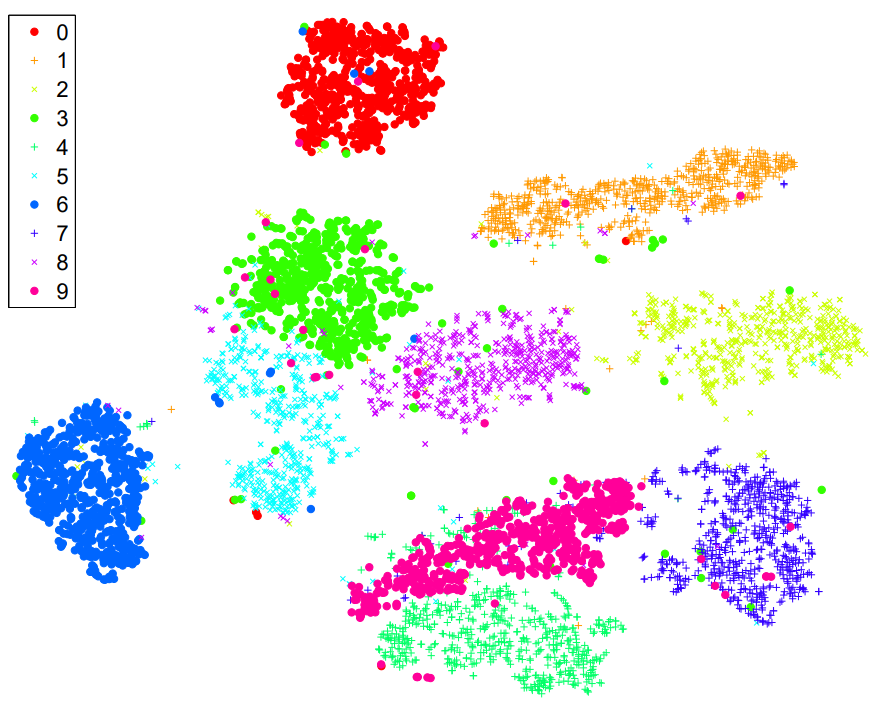
\includegraphics[width=\linewidth]{images/t-sne1.png}
        \caption{Visualization by t-SNE.}
        \label{fig:tsne_mnist_basic_tsne}
    \end{subfigure}
    \hfill
    \begin{subfigure}{0.45\textwidth}
        \centering
        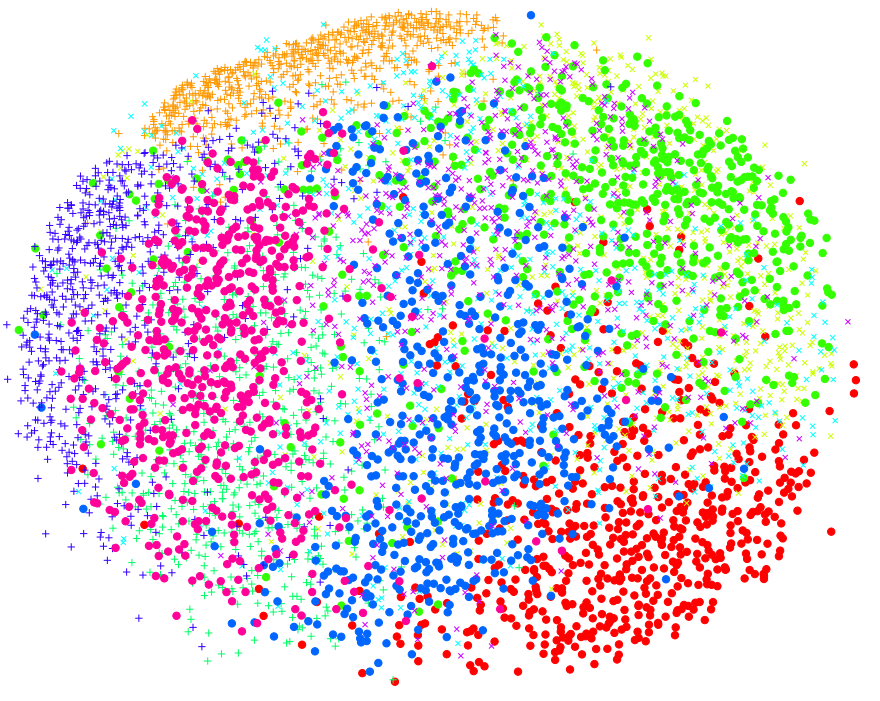
\includegraphics[width=\linewidth]{images/t-sne2.png}
        \caption{Visualization by Sammon mapping.}
        \label{fig:tsne_mnist_basic_sammon}
    \end{subfigure}
    \caption{Comparative visualization of 6,000 handwritten digits from the MNIST dataset using t-SNE (left) and Sammon mapping (right). The t-SNE visualization demonstrates superior cluster separation with clearly distinguishable digit groups (0-9), while Sammon mapping shows significant overlap between different digit classes. This comparison illustrates t-SNE's exceptional capability in preserving local neighborhood structures and creating meaningful cluster formations.}
    \label{fig:tsne_mnist_basic}
\end{figure}

The algorithmic foundation of t-SNE rests on converting high-dimensional Euclidean distances between data points into conditional probabilities that represent similarities. For each data point $x_i$, the algorithm defines the conditional probability $p_{j|i}$ that $x_i$ would select $x_j$ as its neighbor if neighbors were chosen proportionally to their probability density under a Gaussian centered at $x_i$ \cite{maaten2008tsne}. This probability is computed as $p_{j|i} = \frac{\exp(-\|x_i - x_j\|^2/2\sigma_i^2)}{\sum_{k \neq i} \exp(-\|x_i - x_k\|^2/2\sigma_i^2)}$, where $\sigma_i$ represents the variance of the Gaussian kernel around point $x_i$, determined by the perplexity parameter that controls the effective number of nearest neighbors considered for each point.

A crucial aspect of t-SNE is its use of Cauchy distributions to model similarities in the low-dimensional space, rather than the Gaussian distribution used in the high-dimensional space \cite{maaten2008tsne}. 
This heavy-tailed distribution enables moderate distances in the high-dimensional space to be faithfully represented by much larger distances in the low-dimensional map, effectively eliminating unwanted attractive forces between dissimilar points that would otherwise be crowded together in the visualization.

The algorithm operates by minimizing the Kullback-Leibler divergence between the joint probability distributions in high-dimensional and low-dimensional spaces: $C = \sum_i \sum_j p_{i|j} \log \frac{p_{i|j}}{q_{i|j}}$, where $p_{i|j}$ and $q_{i|j}$ represent the joint probabilities in high and low dimensions respectively \cite{maaten2008tsne}. 

t-SNE demonstrates exceptional capability in preserving local neighborhood structures, making it particularly effective for revealing cluster formations and local patterns within high-dimensional data \cite{yang2021dimensionality, maaten2008tsne}. As clearly shown in Figures \ref{fig:tsne_mnist_basic}
the algorithm's focus on modeling local similarities through the perplexity parameter, which allows it to adapt to varying local densities in the data, ensuring that each data point contributes meaningfully to the cost function regardless of its position relative to the global distribution \cite{maaten2008tsne}. 
The perplexity parameter serves as the primary hyperparameter controlling t-SNE's behavior, effectively determining the balance between local and global aspects of the data that are preserved in the embedding \cite{maaten2008tsne}. Typical perplexity values range from 5 to 50, with lower values emphasizing very local structures and higher values incorporating more global relationships. The algorithm's performance exhibits robustness across different perplexity settings for the same dataset, though optimal values may vary depending on the intrinsic structure and size of the data.

The algorithm excels at revealing structure at multiple scales simultaneously, making it particularly valuable for complex high-dimensional datasets that contain hierarchical or nested cluster structures \cite{maaten2008tsne}. This multi-scale capability emerges from t-SNE's probabilistic framework, which naturally adapts to local data densities while maintaining the ability to reveal broader organizational patterns through the heavy-tailed distribution in the embedding space

However, t-SNE exhibits several inherent limitations that impact its applicability in certain contexts. The algorithm's emphasis on preserving local structure can sometimes come at the expense of global relationships, potentially leading to visualizations where the relative positions of distinct clusters may not accurately reflect their relationships in the original high-dimensional space \cite{maaten2008tsne}.

For
% $\text{LORE}_{sa}$ 
neighborhood visualization applications, t-SNE's strength in local structure preservation makes it particularly valuable for revealing fine-grained patterns and cluster formations within synthetic neighborhoods. The algorithm's ability to create clear visual separation between different regions of the feature space can help users understand how 
% $\text{LORE}_{sa}$'s 
surrogate models
local explanations relate to the underlying data distribution. 

% % SET random_state param
% The stochastic nature of t-SNE's optimization means that multiple runs may produce visually different embeddings, though the overall cluster structures typically remain consistent \cite{maaten2008tsne}. This variability necessitates careful interpretation when using t-SNE for exploratory analysis of explanation neighborhoods, as the specific spatial arrangement of points may vary while preserving the essential local neighborhood relationships that define the clustering structure.

\subsubsection{UMAP (Uniform Manifold Approximation and Projection)}

Uniform Manifold Approximation and Projection (UMAP) represents a novel manifold learning technique for dimensionality reduction that differentiates itself through strong theoretical foundations rooted in Riemannian geometry and algebraic topology \cite{mcinnes2020umap}. Unlike many dimensionality reduction algorithms that rely primarily on empirical design decisions, UMAP's construction is grounded in mathematical theory, particularly drawing from the work of Spivak on categorical approaches to geometric realization of fuzzy simplicial sets \cite{mcinnes2020umap, Spivak2009METRICRO}.

UMAP's theoretical framework begins with the assumption that data lies approximately on a locally connected Riemannian manifold, and that this manifold is equipped with a Riemannian metric with respect to which the data is uniformly distributed \cite{mcinnes2020umap}. Building on these foundational assumptions, the algorithm operates by constructing local manifold approximations around each data point through two main processes: approximating the manifold on which the data lies, and constructing fuzzy simplicial set representations of the approximated manifold. 

The algorithm subsequently patches together their local fuzzy simplicial set representations to build a topological representation of the high-dimensional data \cite{mcinnes2020umap}. This approach allows UMAP to capture both local neighborhood structures and global topological relationships within the data, with the local connectivity assumption ensuring that each point is connected to its nearest neighbor with maximum membership strength, maintaining topological consistency across the embedding. The algorithm optimizes the low-dimensional embedding layout by minimizing the cross-entropy between the topological representations of the high-dimensional and low-dimensional spaces, effectively preserving the essential geometric and topological properties of the original data manifold.

One of UMAP's most significant advantages lies in its computational efficiency and embedding stability. To demonstrate this stability advantage, Figure~\ref{fig:umap_tsne_stability} presents a Procrustes-based alignment comparison between UMAP and t-SNE embeddings using subsampled data from a flow cytometry dataset \cite{mcinnes2020umapuniformmanifoldapproximation}. The visualization reveals a critical difference in algorithmic robustness: UMAP maintains substantially better structural consistency between the full dataset (blue points) and a 10\% subsample (red points), as evidenced by the tight alignment and minimal deviation between the two point sets. In contrast, t-SNE exhibits considerable variation in embedding structure when working with subsampled data, with red and blue points showing significant displacement and structural distortion.

\begin{figure}
    \centering
    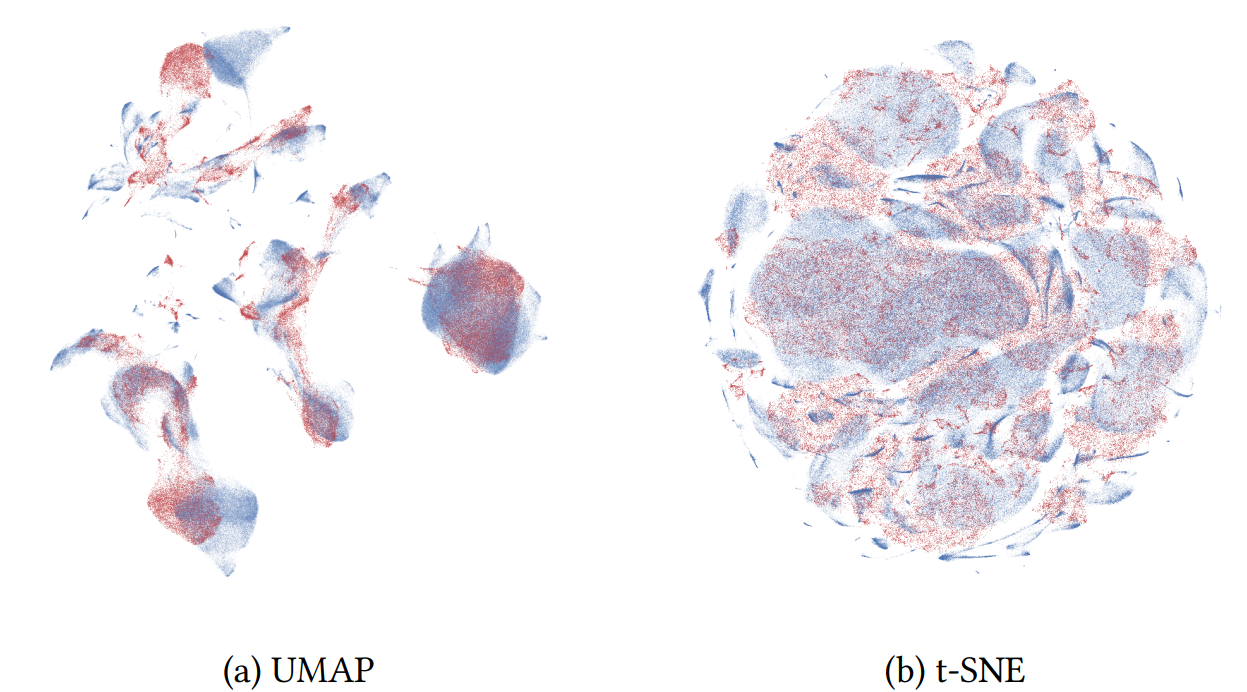
\includegraphics[width=0.8\textwidth]{images/umap.png}
    \caption{
    Procrustes-based alignment comparison of UMAP (left) and t-SNE (right) embeddings on flow cytometry data. Red points represent a 10\% subsample, blue points represent the full dataset \cite{mcinnes2020umapuniformmanifoldapproximation}.}
    \label{fig:umap_tsne_stability}
\end{figure}

One of UMAP's most significant advantages lies in its computational efficiency and scalability. Empirical evaluations demonstrate that UMAP is approximately an order of magnitude faster than t-SNE while maintaining comparable or superior visualization quality. The algorithm exhibits superior scaling performance across multiple dimensions: it scales efficiently with the number of data points, performs exceptionally well with high ambient dimensionality, and maintains computational efficiency when generating embeddings into dimensions higher than two. Unlike t-SNE, which requires global normalization and space trees that scale exponentially with embedding dimension, UMAP represents data as a fuzzy topological structure, allowing it to work without such computationally expensive constructs.

The algorithm's ability to preserve both local and global structure makes it particularly well-suited for interactive visualization applications in eXplainable AI. UMAP successfully maintains local cluster structures that facilitate identification of similar instances in synthetic neighborhoods, while simultaneously preserving global relationships that help users understand the overall data distribution and inter-cluster relationships \cite{becht2019evaluation}. 

UMAP's hyperparameters provide intuitive control over the embedding characteristics. The \texttt{n\_neighbors} parameter controls the balance between local and global structure preservation, with lower values emphasizing local structure and higher values focusing on global relationships. The \texttt{min\_dist} parameter controls the minimum distance between points in the low-dimensional representation, affecting the tightness of clusters in the final embedding \cite{mcinnes2020umap}. These parameters allow users to fine-tune the visualization based on their specific analytical requirements and the characteristics of the synthetic neighborhood being explored.

For 
synthetic
% $\text{LORE}_{sa}$'s 
neighborhood visualization requirements, UMAP's combination of theoretical rigor, computational efficiency, structure preservation, and stability makes it an ideal choice for projecting high-dimensional synthetic neighborhoods into interpretable 2D representations that facilitate effective human-AI interaction and explanation understanding.

\subsubsection{Comparative Analysis of Dimensionality Reduction Techniques}
Recent empirical research has provided comprehensive comparative evaluations of dimensionality reduction techniques across large-scale datasets, offering valuable insights for their application in eXplainable AI systems. Yang et al.\cite{yang2021dimensionality} conducted a systematic comparison of the four dimensionality reduction methods previously discussed: UMAP, t-SNE, PCA, and MDS, across 71 bulk transcriptomic datasets, evaluating their performance through both quantitative metrics and qualitative biological interpretability. This comparative analysis provides crucial evidence for selecting appropriate dimensionality reduction techniques.

The comprehensive evaluation framework uses quantitative metrics including \textbf{clustering accuracy} measured through Normalized Mutual Information (NMI) and Adjusted Rand Index (ARI), \textbf{neighborhood preservation} assessed via Jaccard index, and \textbf{computational efficiency} across varying dataset sizes \cite{yang2021dimensionality}.. 
As shown in Figure \ref{fig:DRcomparison1}, UMAP identified clustering structures in 41 out of 71 datasets (58\%), outperforming both t-SNE (37/71, 52\%), MDS (13/71, 18\%) and PCA (11/71, 15\%).

\begin{figure}
    \centering
    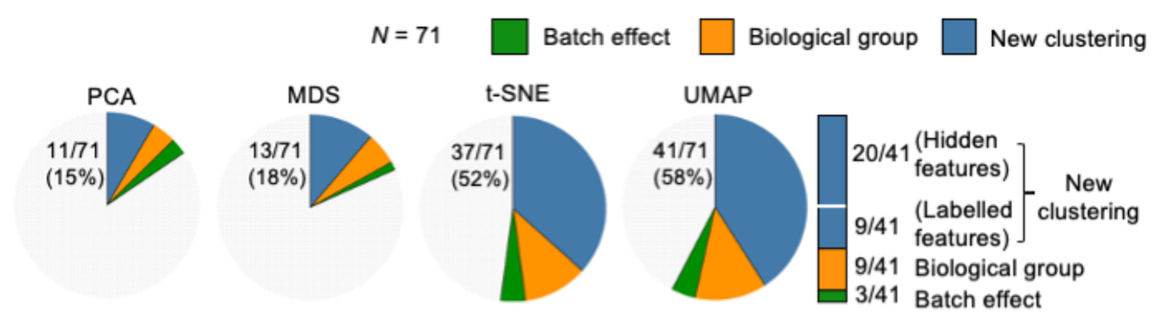
\includegraphics[width=\linewidth]{images/DRcomparison1.png}
    \caption{Dimensionality reduction techniques comparison results.}
    \label{fig:DRcomparison1}
\end{figure}

\paragraph{UMAP vs t-SNE}
The comparison between UMAP and t-SNE reveals complementary strengths, with UMAP demonstrating superior overall performance in large-scale data analysis. Both methods excel at preserving local neighborhood structures, with UMAP achieving an average neighborhood preservation score of 0.35 ± 0.091 compared to t-SNE's 0.36 ± 0.095, indicating comparable local structure retention capabilities \cite{yang2021dimensionality}. As shown in Figure \ref{fig:DRcomparison2}, both techniques substantially outperform linear methods in maintaining local relationships within high-dimensional data.

\begin{figure}
    \centering
    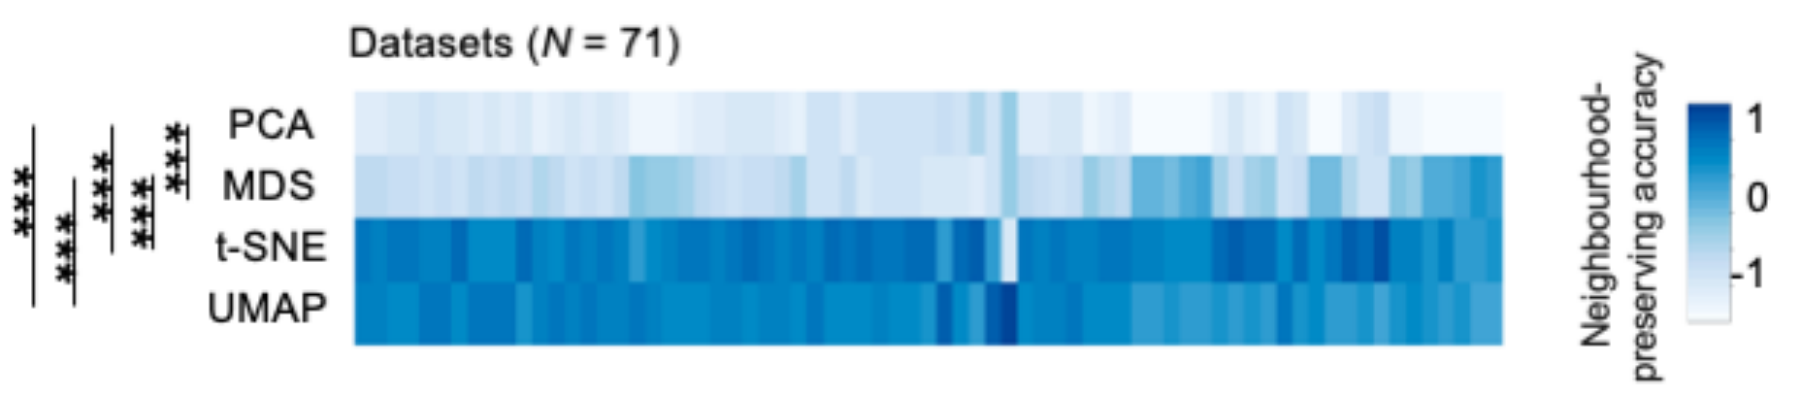
\includegraphics[width=\linewidth]{images/DRcomparison2.png}
    \caption{Dimensionality reduction techniques comparison results on neighborhood-preservation accuracy metric.}
    \label{fig:DRcomparison2}
\end{figure}

However, UMAP demonstrates superior clustering accuracy across multiple evaluation criteria. Figure \ref{fig:DRcomparison3} illustrates how UMAP consistently achieved the highest Normalized Mutual Information scores across five different clustering algorithms (k-means, hierarchical clustering, spectral clustering, Gaussian mixture model, and HDBSCAN), while t-SNE ranked second but with notably lower performance. 

\begin{figure}
    \centering
    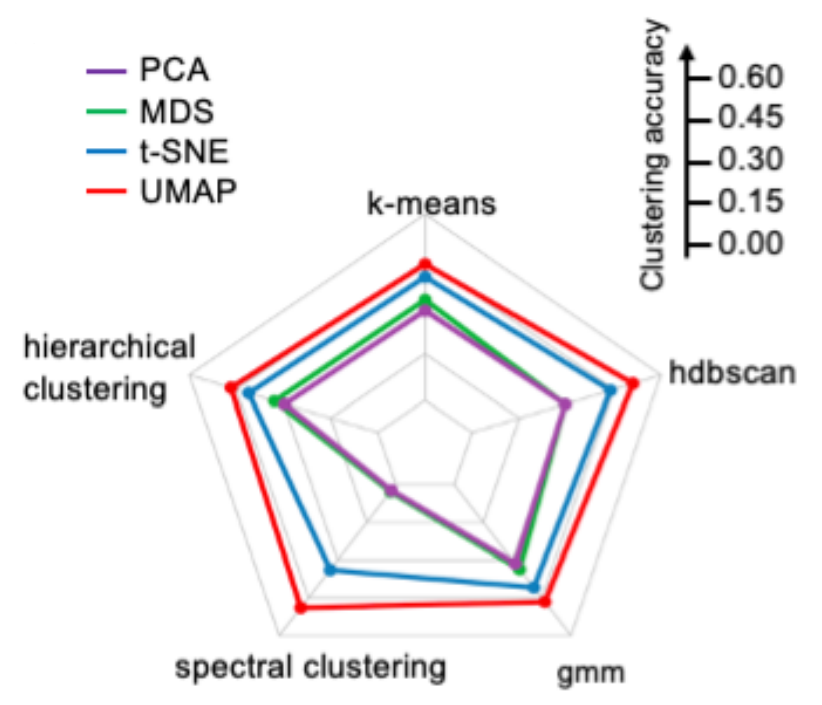
\includegraphics[width=0.7\linewidth]{images/DRcomparison3.png}
    \caption{Dimensionality reduction techniques comparison results on Normalized Mutual Information scores across five different clustering algorithms.}
    \label{fig:DRcomparison3}
\end{figure}

This enhanced clustering accuracy translates directly to improved separability of meaningful data structures, with UMAP achieving over 90\% random forest classification accuracy for batch effect detection compared to t-SNE's slightly lower performance.
A critical advantage of UMAP over t-SNE lies in computational efficiency, particularly for large-scale datasets. 
While both methods perform similarly for smaller datasets (200-500 samples), UMAP gains substantial advantages as dataset size increases. For datasets with 10,000 samples, UMAP requires approximately 3 minutes compared to t-SNE's 1.5 hours, representing more than a 25-fold improvement in computational speed. This efficiency advantage makes UMAP significantly more practical for interactive explanation systems that require responsive visualization updates.
Additionally, UMAP exhibits superior global structure preservation compared to t-SNE, arising from its use of Laplacian Eigenmap initialization and cross-entropy objective function rather than t-SNE's random initialization and KL-divergence approach \cite{yang2021dimensionality}. 

\paragraph{UMAP vs PCA}
The comparison between UMAP and PCA highlights fundamental differences between nonlinear manifold learning and linear dimensionality reduction approaches. While PCA demonstrates superior computational efficiency, processing 10,000 samples in approximately 20 seconds compared to UMAP's 3 minutes \cite{yang2021dimensionality}, UMAP provides dramatically superior performance in revealing complex data structures and meaningful clustering patterns.
The most striking difference appears in clustering structure identification capabilities. As demonstrated in Figure \ref{fig:DRcomparison1}, PCA identified clustering structures in only 11 out of 71 datasets (15\%), while UMAP revealed structures in 41 datasets (58\%). This improvement in structure detection capability is due to UMAP's ability to capture nonlinear relationships that PCA's linear transformation cannot represent effectively.
Clustering accuracy metrics reveal substantial performance differences between the methods. Figure \ref{fig:DRcomparison2} shows UMAP achieving consistently higher NMI scores across all clustering algorithms, while PCA demonstrated the poorest performance among all evaluated methods. This difference extends to neighborhood preservation, where UMAP's local structure retention (0.35 ± 0.091) significantly exceeds PCA's performance (0.19 ± 0.067), indicating that PCA's linear projections fail to maintain the local relationships crucial for interactive data exploration.
Despite PCA's computational advantages and interpretability through component loadings, its fundamental limitation lies in the linear assumption that proves inadequate for complex data structures. 

\paragraph{UMAP vs MDS}
The comparison between UMAP and MDS reveals the limitations of classical distance-preserving approaches when applied to complex high-dimensional data. MDS, while theoretically principled in its global distance preservation approach, demonstrates inferior performance across multiple evaluation criteria compared to UMAP's manifold learning methodology.
Computational efficiency represents a significant disadvantage for MDS. 
MDS as the slowest performing method across all dataset sizes, with particularly poor scaling characteristics that make it impractical for large-scale interactive applications. This computational burden severely limits MDS's applicability in explainability systems where responsive visualization updates are essential for effective human-AI interaction.
Clustering accuracy metrics reveal substantial performance gaps between the methods. UMAP consistently outperforms MDS across all clustering algorithms evaluated.
% , with MDS showing particularly poor performance in biological group separation tasks. 
The neighborhood preservation analysis highlights fundamental differences in the methods' design philosophies. While MDS focuses on preserving global pairwise distances, this emphasis comes at the expense of local neighborhood structure preservation. Figure \ref{fig:DRcomparison2} shows MDS achieving only moderate neighborhood preservation (0.26 ± 0.114) compared to UMAP's superior local structure retention (0.35 ± 0.091).
Structure identification capabilities further demonstrate UMAP's superiority. 
For 
% $\text{LORE}_{sa}$ 
synthetic
neighborhoods visualization applications, MDS's focus on global distance preservation may theoretically seem appealing for maintaining quantitative relationships within synthetic neighborhoods. However, the empirical evidence demonstrates that UMAP's superior local structure preservation, computational efficiency, and clustering accuracy make it significantly more suitable for interactive explanation systems where users need to explore and understand complex data relationships efficiently.

Figure \ref{fig:Dimensionality reduction webapp example} illustrates the comparison of the 4 methods on the same generated neighborhood of 3000 samples.

\begin{figure}[!ph]
    \centering

    \begin{subfigure}[c]{0.48\linewidth}
        \centering
        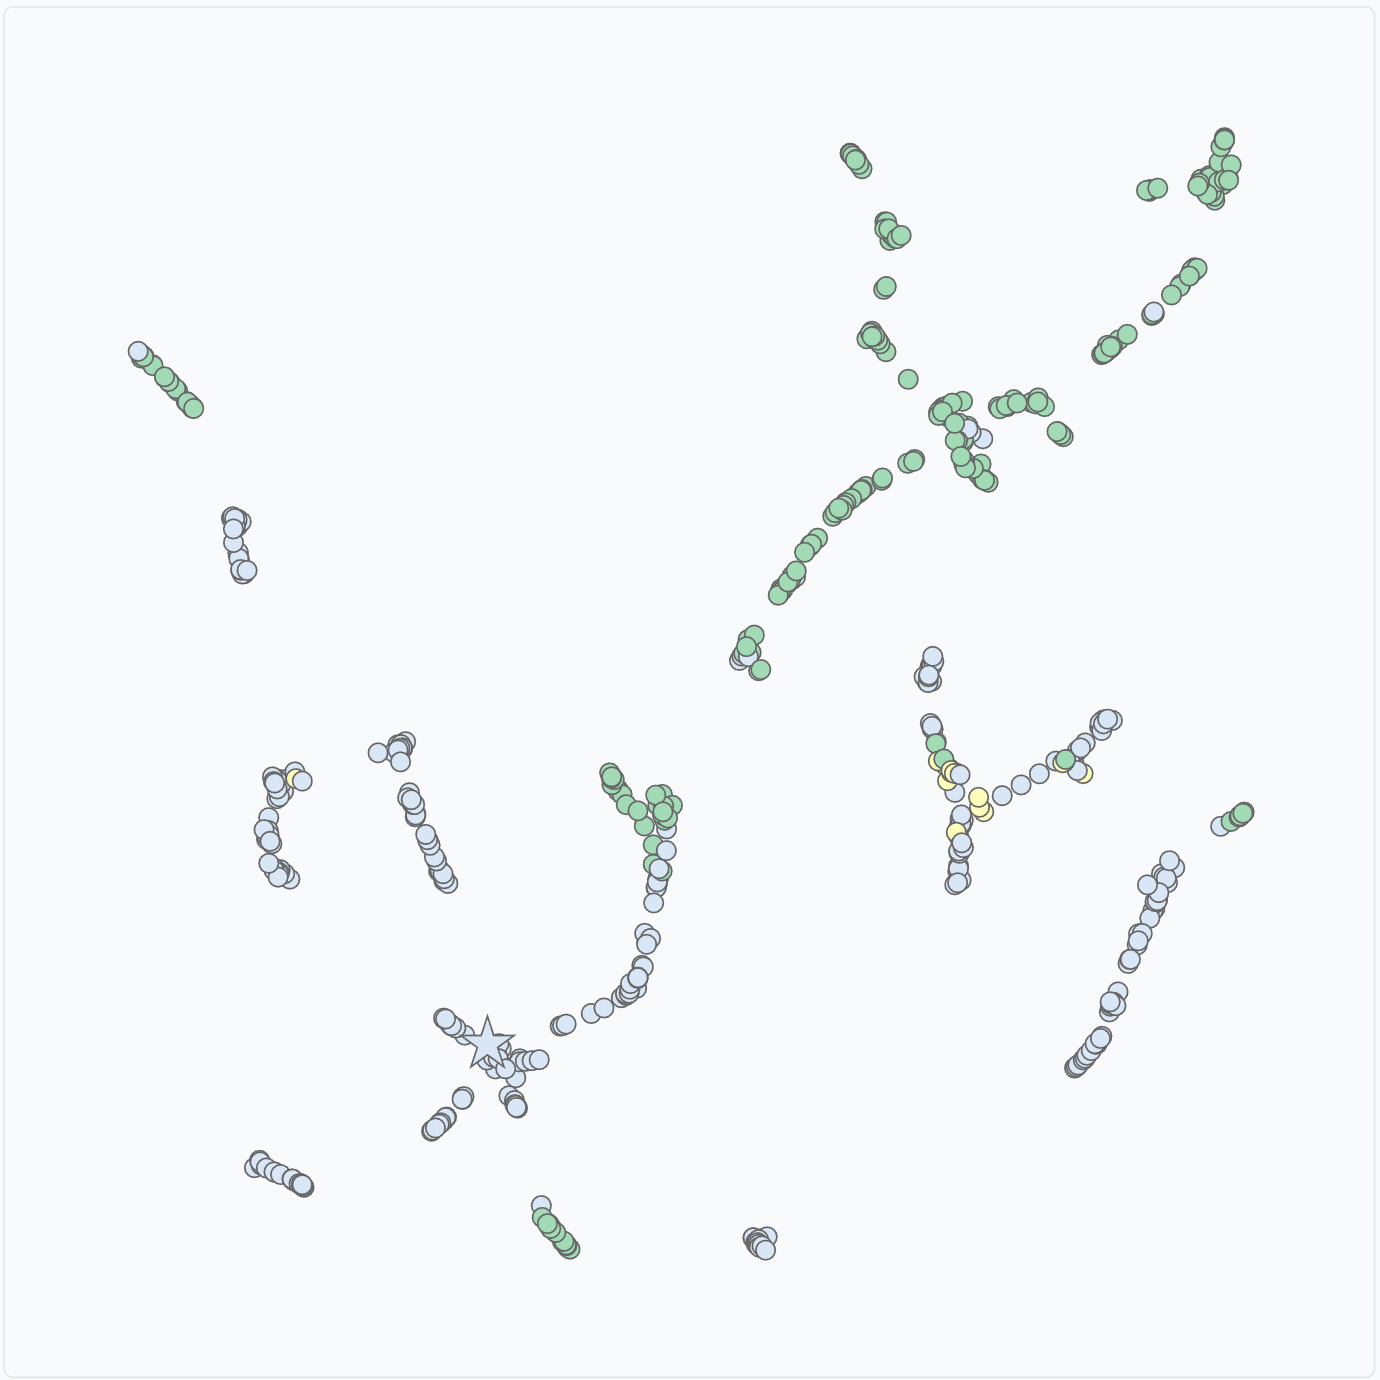
\includegraphics[width=\linewidth]{images/DR example UMAP.png}
        \caption{Uniform Manifold Approximation and Projection for dimension reduction}
        \label{fig:DR example UMAP}
    \end{subfigure}
    \hfill
    \begin{subfigure}[c]{0.48\linewidth}
        \centering
        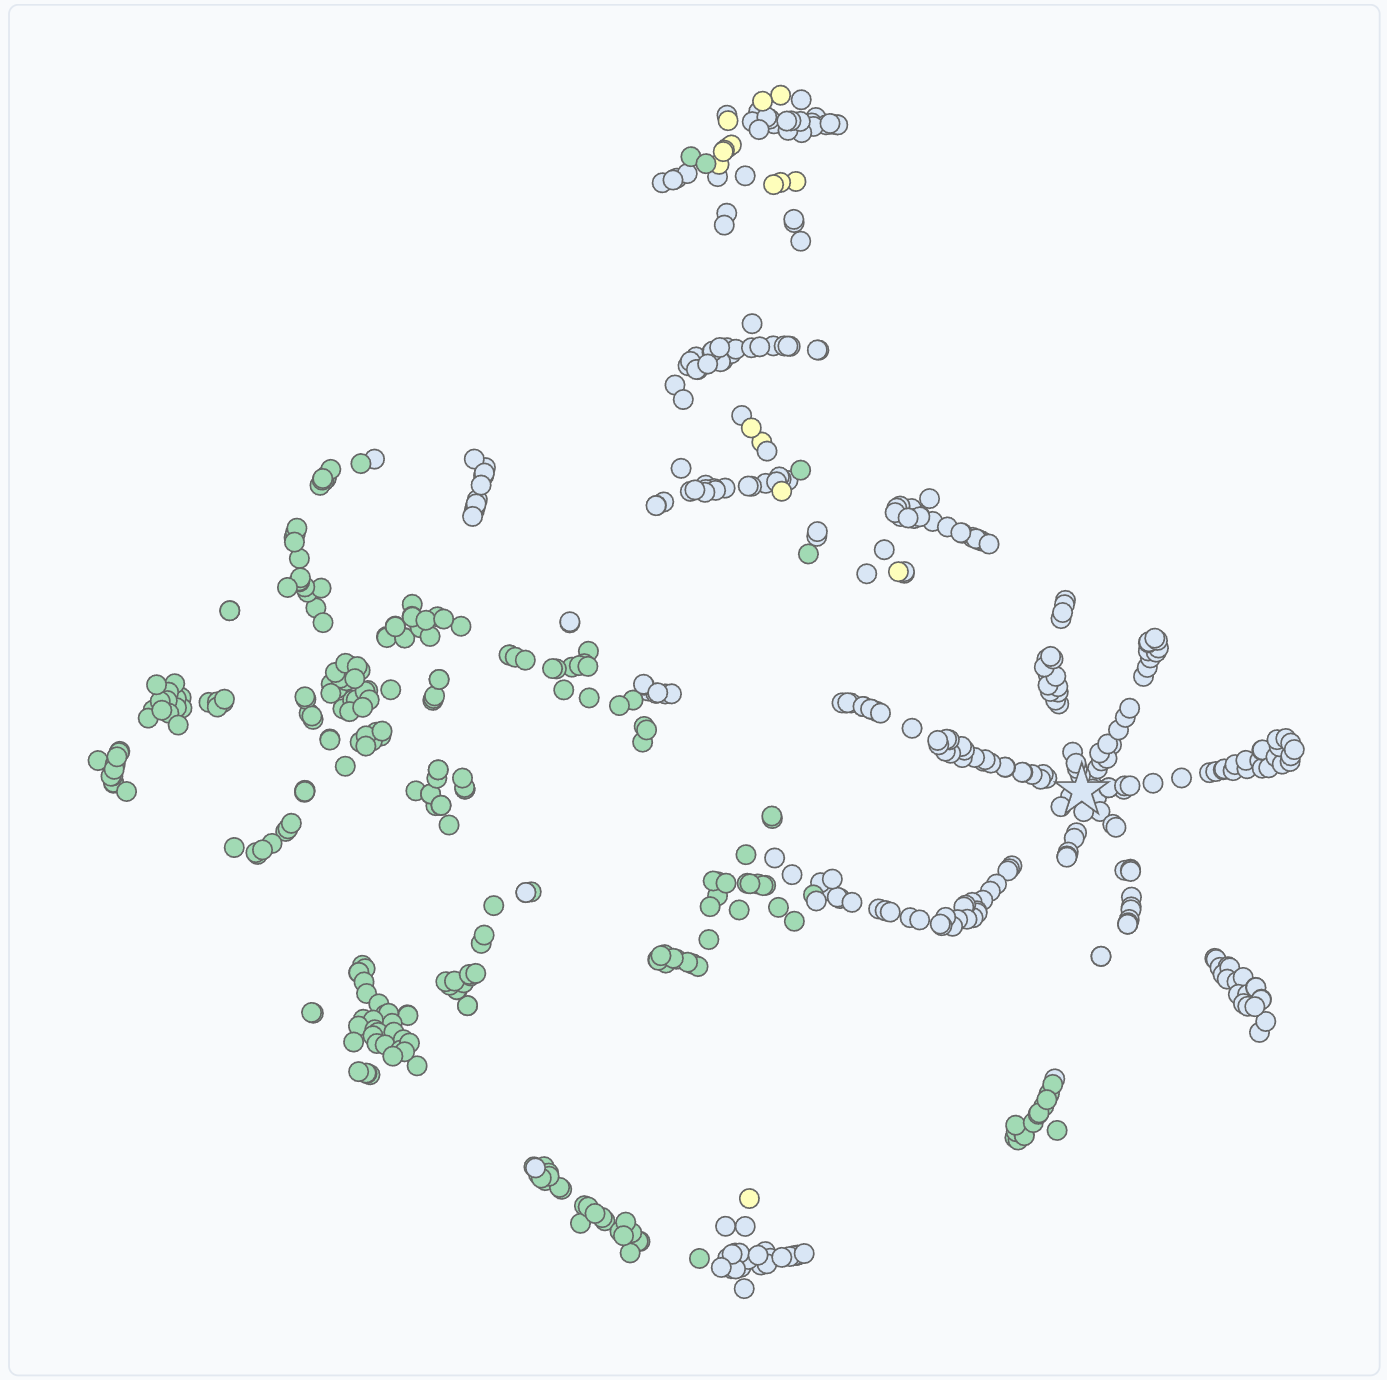
\includegraphics[width=\linewidth]{images/DR example t-sne.png}
        \caption{t-distributed Stochastic Neighbor Embedding}
        \label{fig:DR example t-SNE}
    \end{subfigure}
    
    \vspace{0.1cm} 

    \begin{subfigure}[c]{0.48\linewidth}
        \centering
        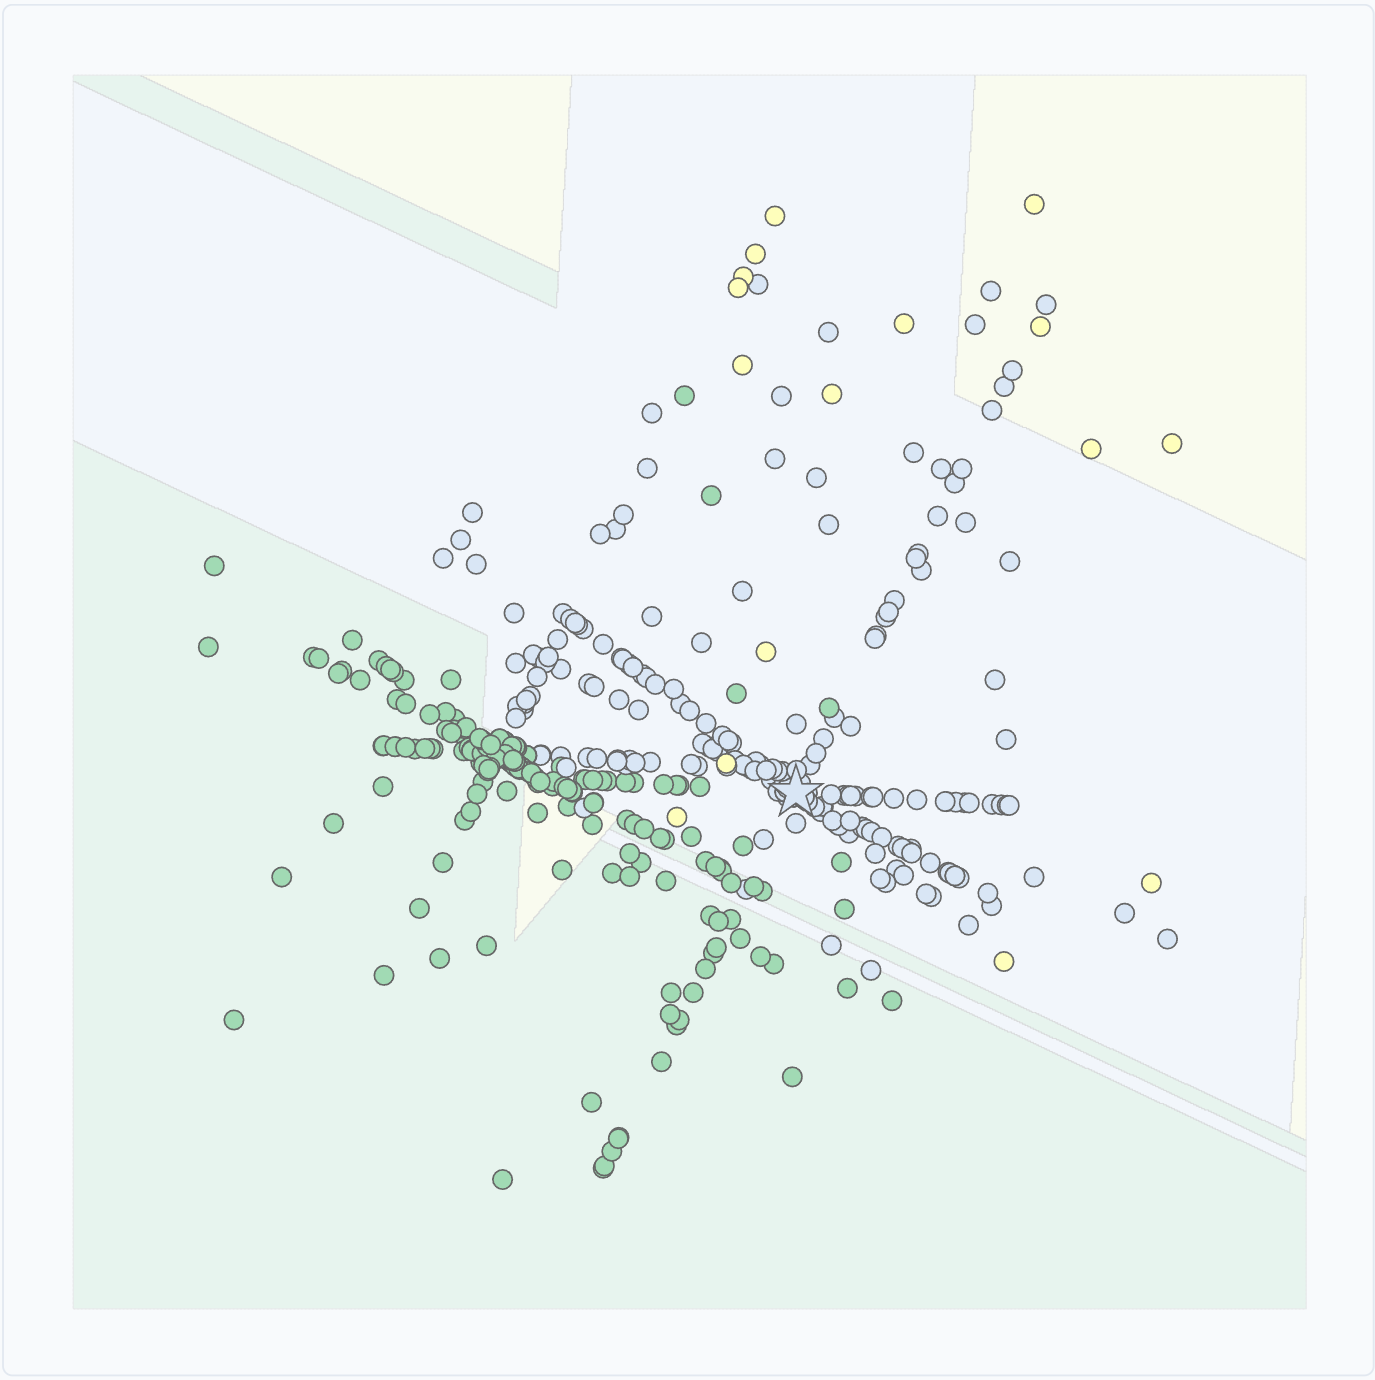
\includegraphics[width=\linewidth]{images/DR example PCA.png}
        \caption{Principal Component Analysis}
        \label{fig:DR example PCA}
    \end{subfigure}
    \hfill
    \begin{subfigure}[c]{0.48\linewidth}
        \centering
        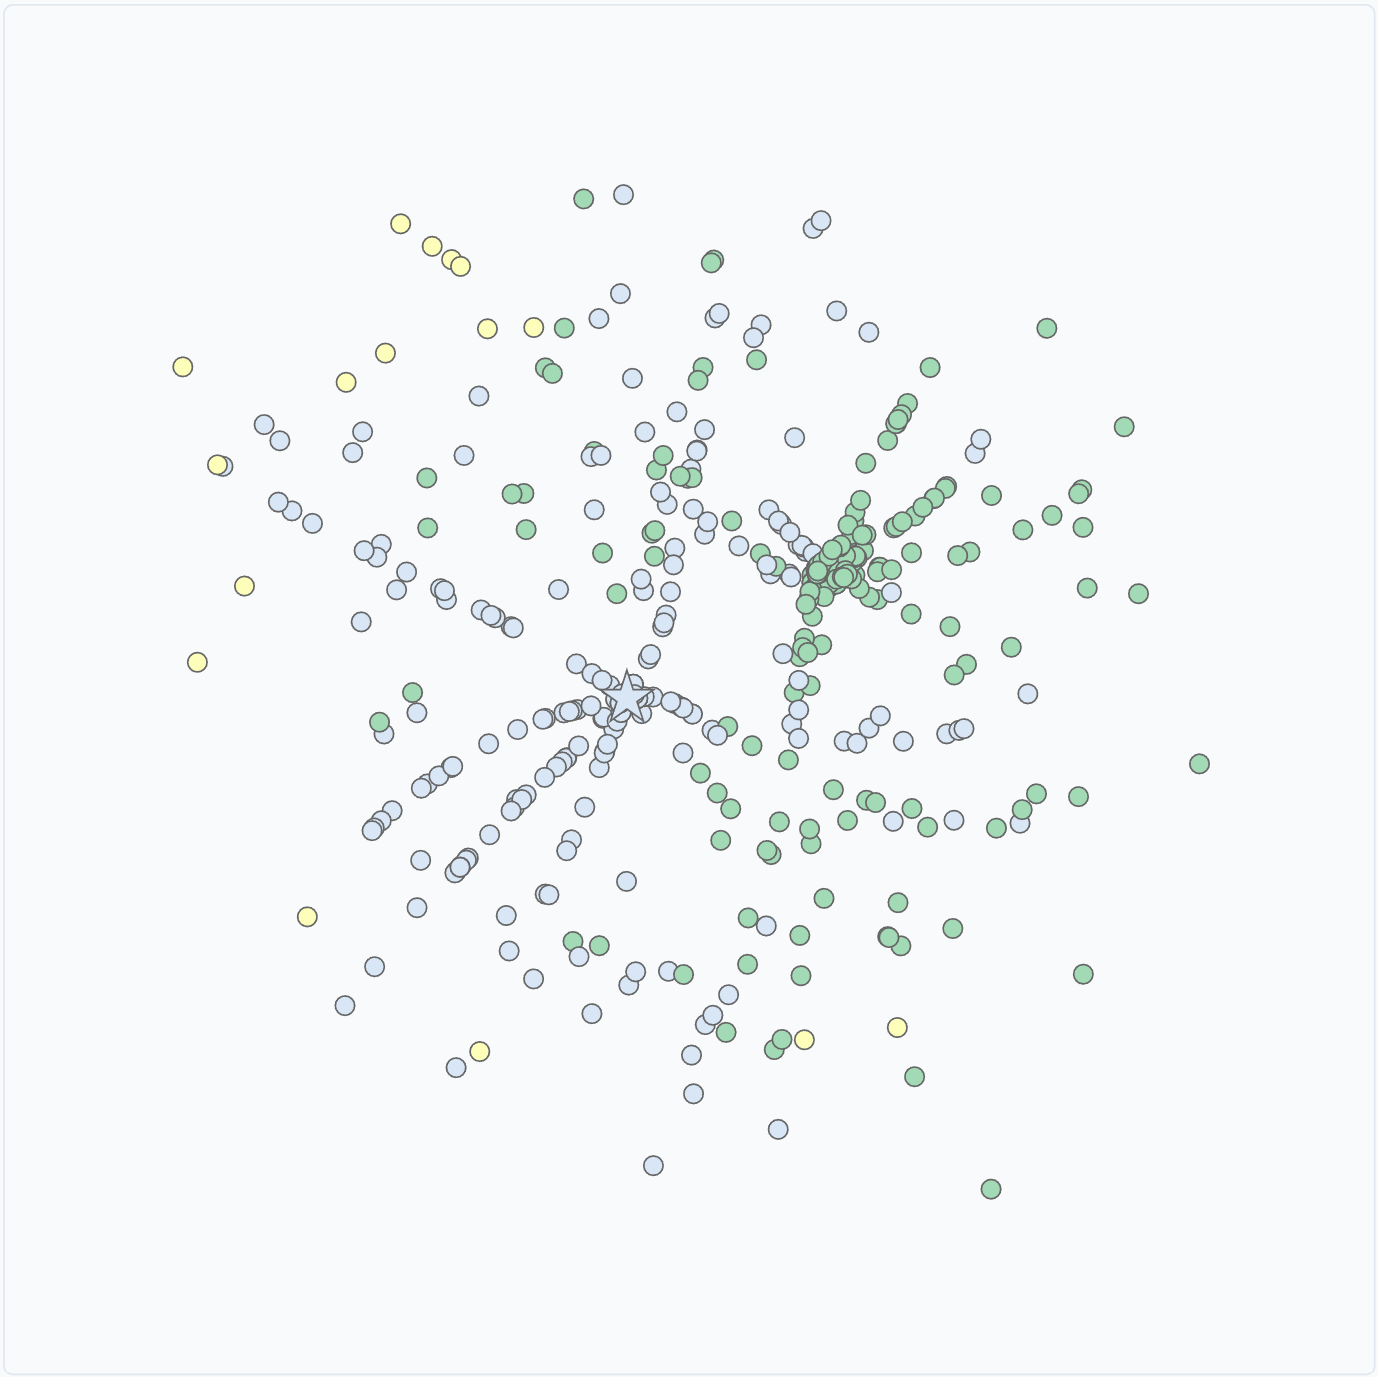
\includegraphics[width=\linewidth]{images/DR example MDS.png}
        \caption{MultiDimensional Scaling}
        \label{fig:DR example MDS}
    \end{subfigure}
    
    \caption{Example of the four dimensionality reduction techniques on a $\text{LORE}_{sa}$ generated neighborhood of 3000 samples, generated starting from the mean instance of the IRIS dataset}
    \label{fig:Dimensionality reduction webapp example}
\end{figure}
        \subsection{Decision Trees}
        

Decision trees have long been recognized as one of the most interpretable machine learning models due to their transparent hierarchical structure and human-readable decision rules \cite{10.1145/2783258.2788613, wang2022timbertrek, lin2022generalizedscalableoptimalsparse, ustun2019learningoptimizedriskscores}. The effective visualization of decision trees for interpretability is an active area of research, with significant implications for eXplainable Artificial Intelligence and human-AI interaction. The challenge extends beyond simply displaying the tree structure to creating interfaces that support comprehensive understanding, analysis, and interaction with both the model and the underlying data.

The literature on decision tree visualization spans 
from traditional node-link diagrams to sophisticated interactive systems. Hans-Jorg Schulz \cite{schulz2011treevis} provides a comprehensive survey identifying over 180 tree visualization techniques, categorizing them by dimensionality (2D, 3D, or hybrid), edge representation (explicit, implicit, or hybrid), and node alignment (radial, axis-parallel, or free). This taxonomic foundation reveals the breadth of approaches available, yet also highlights the fragmented nature of the field, where many techniques have been developed independently without systematic comparison.

Recent advances in the field emphasize the critical importance of integrating visualization with interaction and algorithmic support. Van den Elzen et al. \cite{elzen2011baobabview} demonstrate that effective decision tree systems require tight coupling between these three components, enabling domain experts to incorporate their knowledge into both tree construction and analysis processes. Their BaobabView system, shown in Figure \ref{fig:baobab_interface}, exemplifies this integration by supporting interactive growing, pruning, optimization, and analysis of decision trees through coordinated visual interfaces.

% Source: BaobabView Interactive Construction and Analysis of Decision Trees, Page: Figure 3
\begin{figure}[!htb]
    \centering
    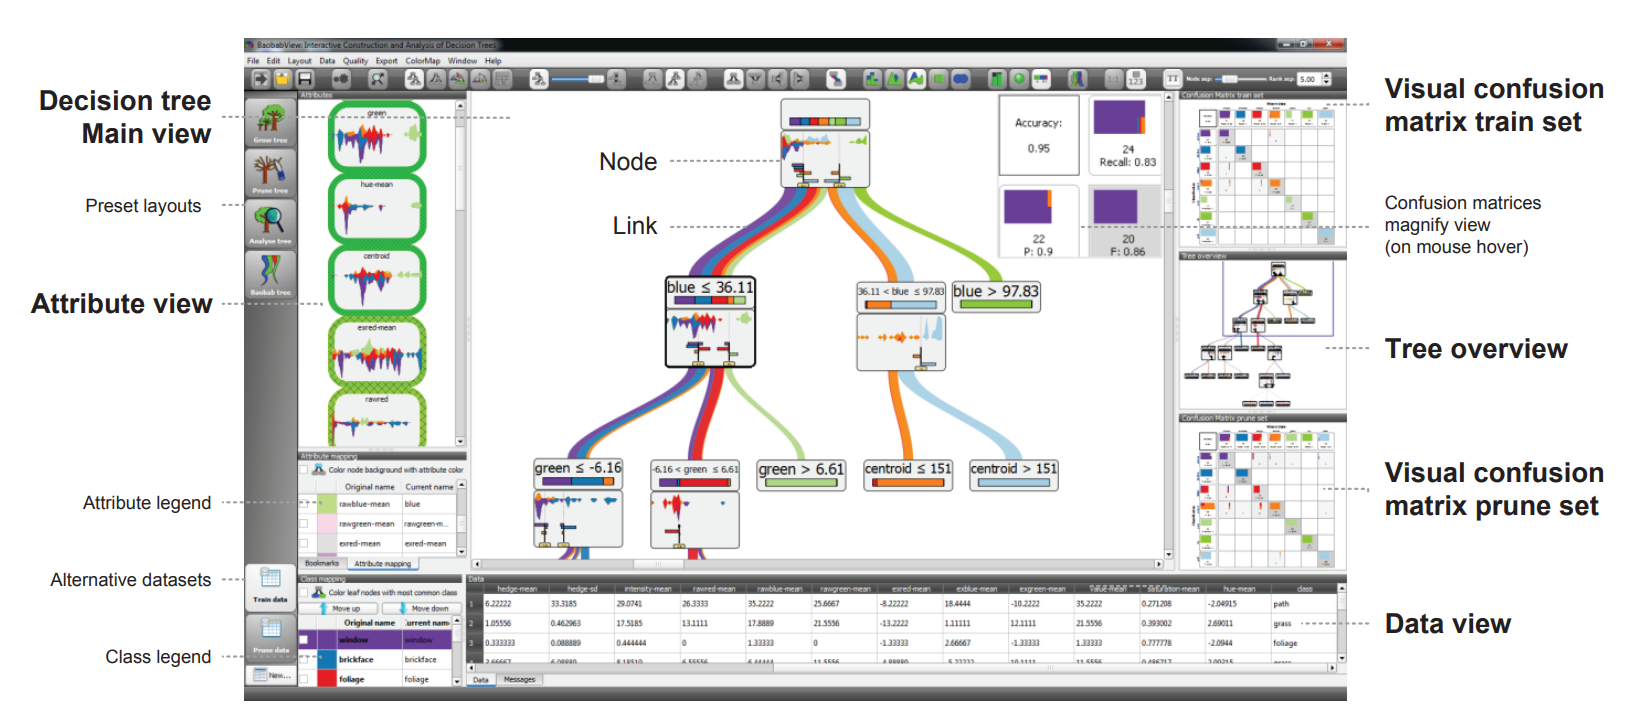
\includegraphics[width=\linewidth]{images/baobabView UI.png}
    \caption{Interface of the interactive decision tree construction software BaobabView with the proposed decision tree visualization. Based on adapted node-link diagram, nodes contain important decision tree components while links are visualized as a stream of items flowing between nodes. The interface integrates decision tree main view, attribute view, visual confusion matrices, tree overview, and data view for comprehensive analysis.}
    \label{fig:baobab_interface}
\end{figure}

The application domains for decision tree visualization are diverse, with particular emphasis on high-stakes decision-making contexts. In medical applications, Jakub Mrva et al. \cite{mrva2019decision} explore 3D visualization techniques that not only display tree structure but also reveal correlations between attributes and decision impacts, as demonstrated in Figure \ref{fig:3d_medical_trees}. 

% Source: Decision Support in Medical Data Using 3D Decision Tree Visualisation, Multiple pages
\begin{figure}
  \centering

  \begin{subfigure}[c]{0.95\textwidth}
    \centering
    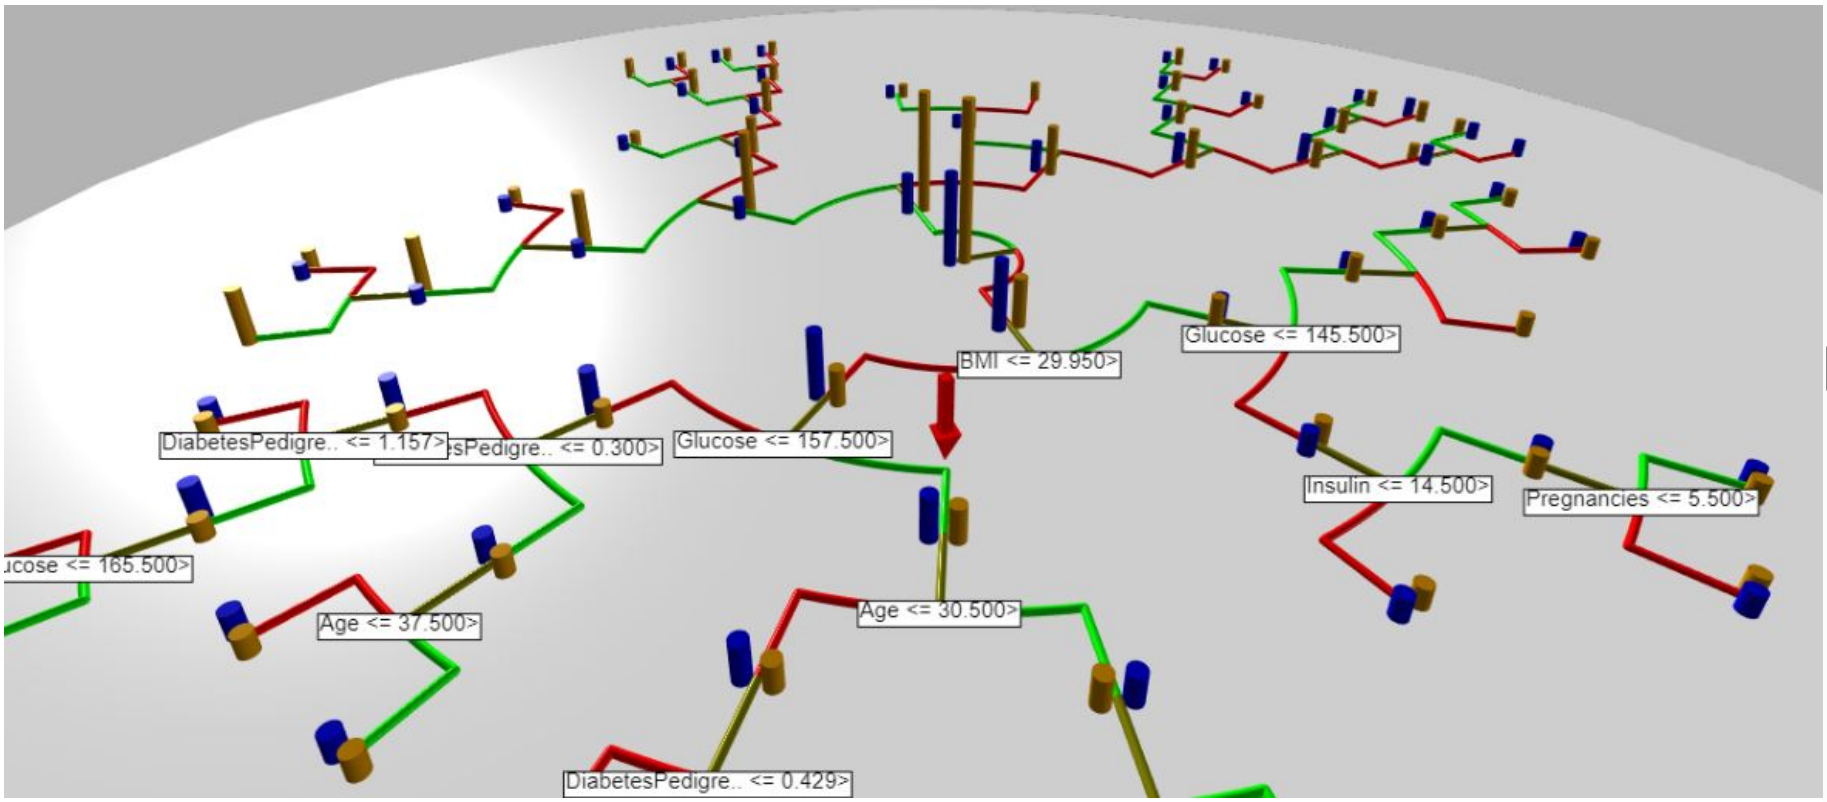
\includegraphics[width=\linewidth]{images/3D Decision Tree1.png}
    \caption{Visualization displaying the overall structure of the trained decision tree on diabetes dataset. Focused node is marked by the arrow.}
    \label{fig:top}
  \end{subfigure}

  \vspace{6pt} 

  \begin{subfigure}[c]{0.48\textwidth}
    \centering
    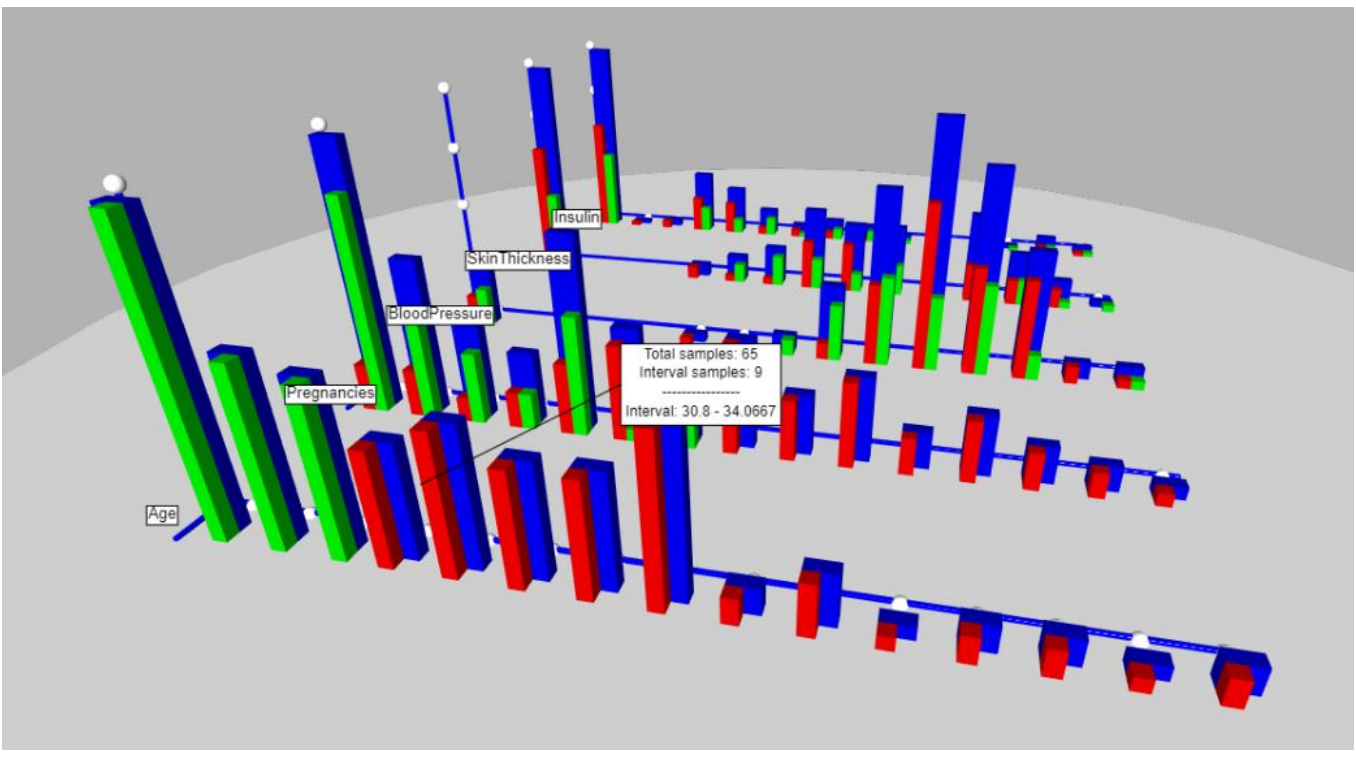
\includegraphics[width=\linewidth]{images/3D Decision Tree2.png} 
    \caption{A focused view on one decision tree node. The first set of histograms
displays attribute used in the split. Following sets display correlated attributes.}
    \label{fig:bottom-left}
  \end{subfigure}
  \hfill
  \begin{subfigure}[c]{0.48\textwidth}
    \centering
    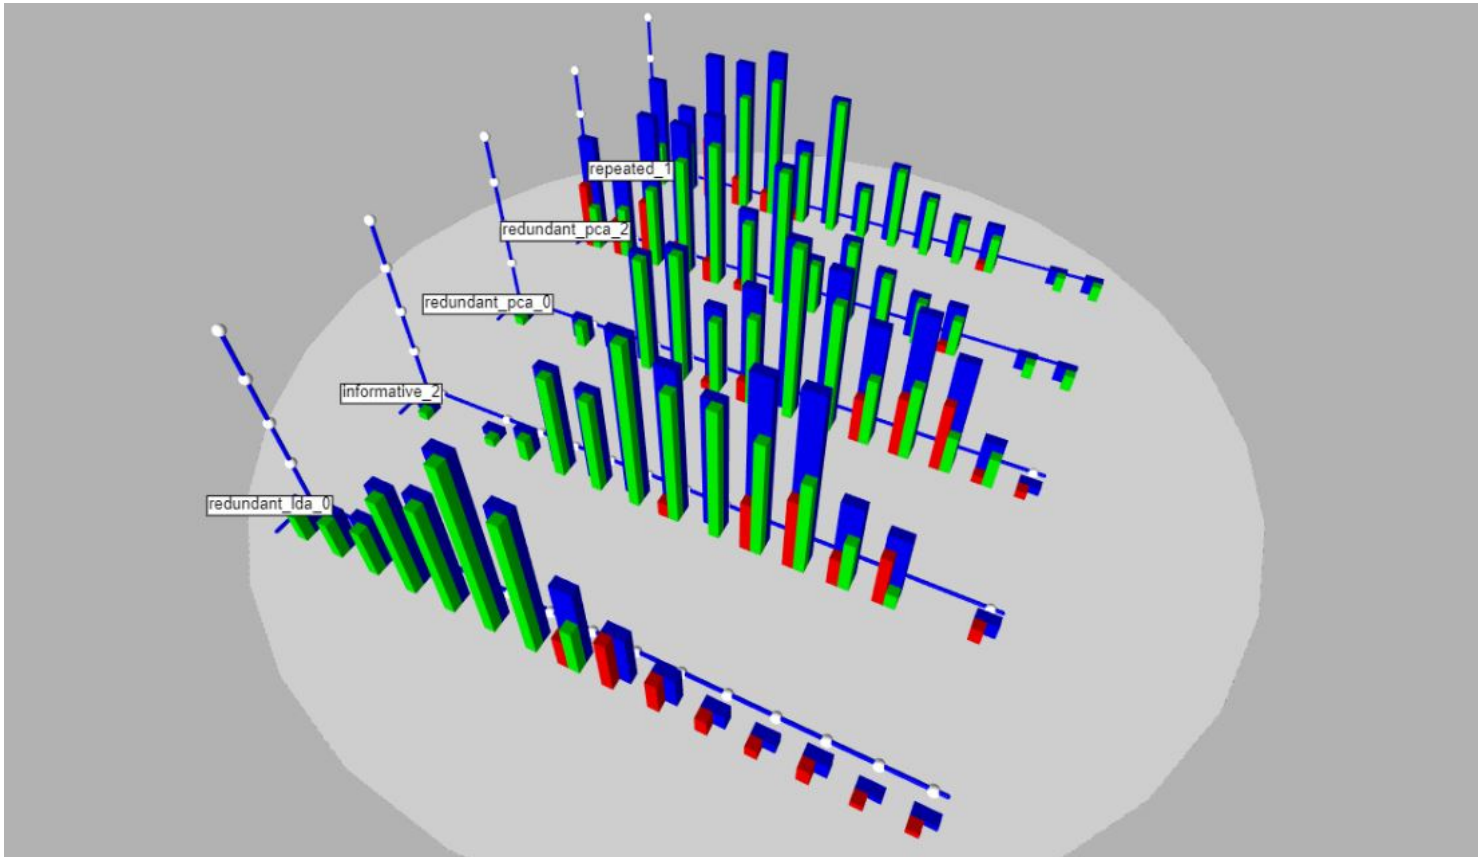
\includegraphics[width=\linewidth]{images/3D Decision Tree3.png}
    \caption{A detailed view on a decision rule in a single node and histograms for
other attribute values of both data subsets divided by the node. Histograms in
decreasing dissimilarity order highlight most important differences. }
    \label{fig:bottom-right}
  \end{subfigure}

    \caption{3D decision tree visualization for medical data using circular plane layout. Nodes are positioned based on depth from the root, with 3D bar charts and histograms showing class distributions and feature relationships. This approach emphasizes visualization of attribute correlations beyond the primary splitting criterion.}
    \label{fig:3d_medical_trees}
\end{figure}

A significant trend in recent literature is the handling of high-dimensional data and complex model spaces. Szücs et al. \cite{szucs2018decision} deal with the challenge of visualizing decision boundaries in high-dimensional feature spaces through projection strategies, while Wang et al. \cite{wang2022timbertrek} address the problem of model selection from large sets of equally-performing trees through their innovative Rashomon set visualization shown in Figure \ref{fig:timbertrek_system}. These works highlight the evolving complexity of decision tree applications and the corresponding need for more sophisticated visualization approaches.

% Source: TimberTrek Exploring and Curating Sparse Decision Trees with Interactive Visualization, Page: Figure 1  
\begin{figure}[ht!]
    \centering
    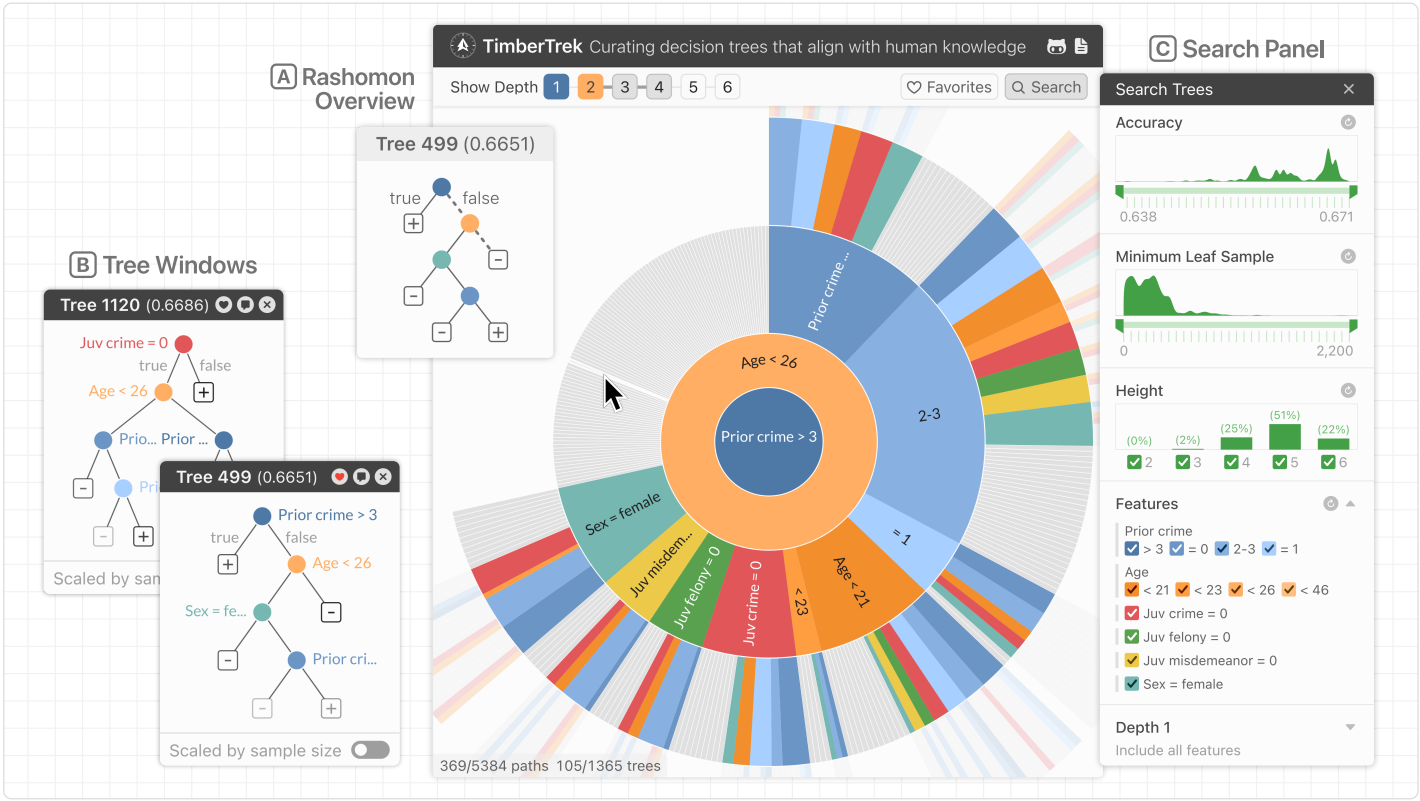
\includegraphics[width=0.95\linewidth]{images/TIMBERTREK .png}
    \caption{TIMBERTREK empowers domain experts and data scientists to easily explore thousands of well-performing decision trees so
they can find and collect those trees that best reflect their knowledge and values. Consider the task of predicting whether a criminal
is likely to commit a crime in the next two years. (A) The Rashomon Overview visually summarizes all well-performing decision trees
by organizing them based on their decision paths, enabling users to seamlessly transition across different model subsets and explore
trees with similar prediction patterns. (B) Clicking a tree opens a repositionable Tree Window showing details of a decision tree:
multiple windows allow users to compare several model candidates’ prediction patterns. (C) The Search Panel provides filtering tools,
enabling users to quickly identify decision trees with desired properties, such as accuracy, robustness, simplicity, and used features.}
    \label{fig:timbertrek_system}
\end{figure}

Interactive capabilities have emerged as a central theme across multiple studies. Kovalerchuk et al. \cite{kovalerchuk2019interactive} demonstrate how interactive threshold modification and dynamic tree construction can enhance model interpretability, while practical tools like dtreeviz \cite{parr2019dtreeviz} focus on providing immediate visual feedback for model validation and debugging. The emphasis on interactivity reflects a broader shift from static visualizations toward dynamic exploration tools that support iterative analysis and refinement.

Despite this rich literature, several gaps remain in current approaches. Most existing visualizations treat the tree structure and the underlying data as separate entities, requiring users to mentally connect model decisions with data distributions. Furthermore, there is limited exploration of how spatial neighborhood analysis plot can be integrated with rule-based interfaces to provide spatial context for
instance-level interpretations. 

\subsubsection{Analysis of Existing Literature and Visualization Techniques}

The literature reveals a diverse ecosystem of decision tree visualization techniques and tools, which can be categorized based on their visual representation approach, interaction paradigm, and target use case. Streeb et al. \cite{Streeb2021TaskBasedVI} provide one of the most comprehensive analyses of this topic, surveying over 150 publications and categorizing them across 16 distinct tasks, 10 possible visual designs, 16 visual designs of further components, and 16 quality measures.
The general results of the evaluation can be observed in Tables \ref{tab:taskStreeb2021TaskBasedVI}, \ref{tab:measureStreeb2021TaskBasedVI} and \ref{tab:VisualDesignsOfTreesANDFurtherComponentsStreeb2021TaskBasedVI}, but the consultation of the publication, currently available at the following link \href{https://el-assady.com/publication/2021streebtask/2021streebtask.pdf}{https://el-assady.com/publication/2021streebtask/2021streebtask.pdf}, is recommended to obtain a full picture of the results and of the reference articles.

{
\footnotesize
\begin{longtable}{|l|*{16}{c|}}
\caption{Tasks \cite{Streeb2021TaskBasedVI}}
\label{tab:taskStreeb2021TaskBasedVI}\\
\hline
\textbf{Ref.} & 
\rotatebox{90}{Concept Introduction} &
\rotatebox{90}{Model Building} &
\rotatebox{90}{Evaluation} &
\rotatebox{90}{Understanding} &
\rotatebox{90}{Diagnosis} &
\rotatebox{90}{Refinement} &
\rotatebox{90}{Comparison} &
\rotatebox{90}{Ensemble Building} &
\rotatebox{90}{Provenance} &
\rotatebox{90}{Reporting} &
\rotatebox{90}{Presentation} &
\rotatebox{90}{Application} &
\rotatebox{90}{Assessment} &
\rotatebox{90}{Monitoring} &
\rotatebox{90}{Decision Modeling} &
\rotatebox{90}{Model Approximation} \\
\hline
\textbf{Total: 152} & 36 & 36 & 34 & 46 & 21 & 8 & 43 & 10 & 3 & 5 & 55 & 6 & 10 & 1 & 11 & 6 \\
\hline
\end{longtable}
}

\begin{table}[ht!]
    \centering
    \caption{Cross-tabulation of tasks and quality measures displayed in the 152 publications Streeb et al. \cite{Streeb2021TaskBasedVI} surveyed. Totals count unique publications in each row/column. Clearly, Accuracy is the most prominently displayed measure of quality. However, compared to the size of our sample quality measures are rarely displayed. There is no relationship apparent between tasks and the quality measures displayed.}
    \label{tab:measureStreeb2021TaskBasedVI}
    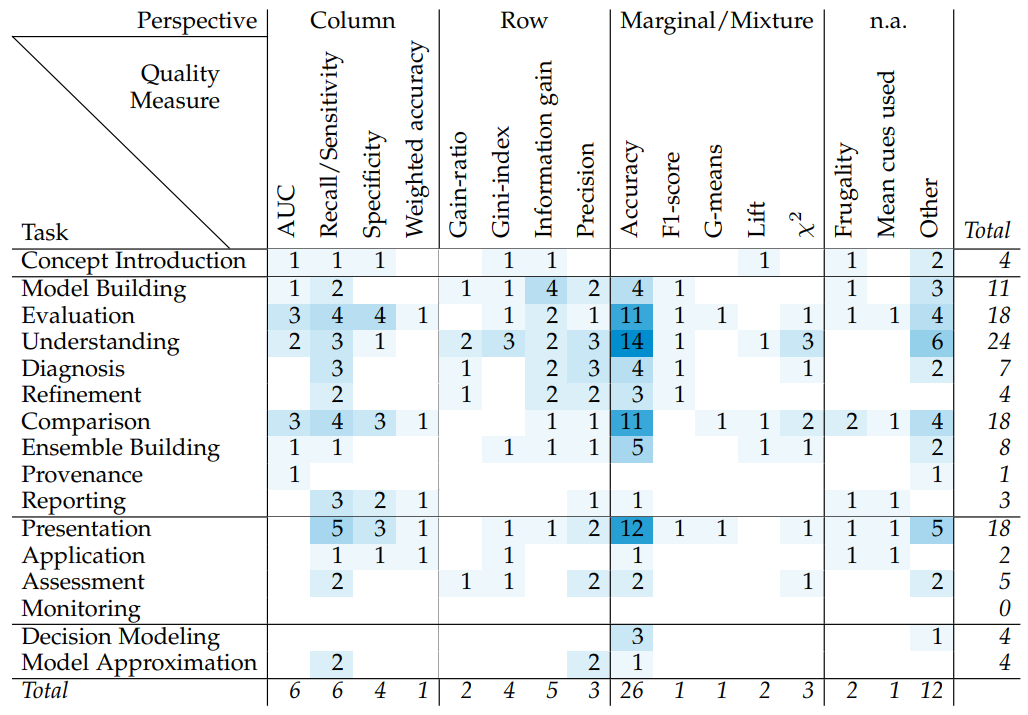
\includegraphics[width=\linewidth]{images/measureStreeb2021TaskBasedVI.png}
\end{table}

\begin{table}
    \centering
    \caption{Cross-tabulation of tasks and quality measures displayed in the 152 publications Streeb et al. \cite{Streeb2021TaskBasedVI} surveyed. Totals count unique publications in each row/column. Clearly, Accuracy is the most prominently displayed measure of quality. However, compared to the size of the analyzed sample, quality measures are rarely displayed. There is no apparent relationship between tasks and the quality measures displayed.}
    \label{tab:VisualDesignsOfTreesANDFurtherComponentsStreeb2021TaskBasedVI}
    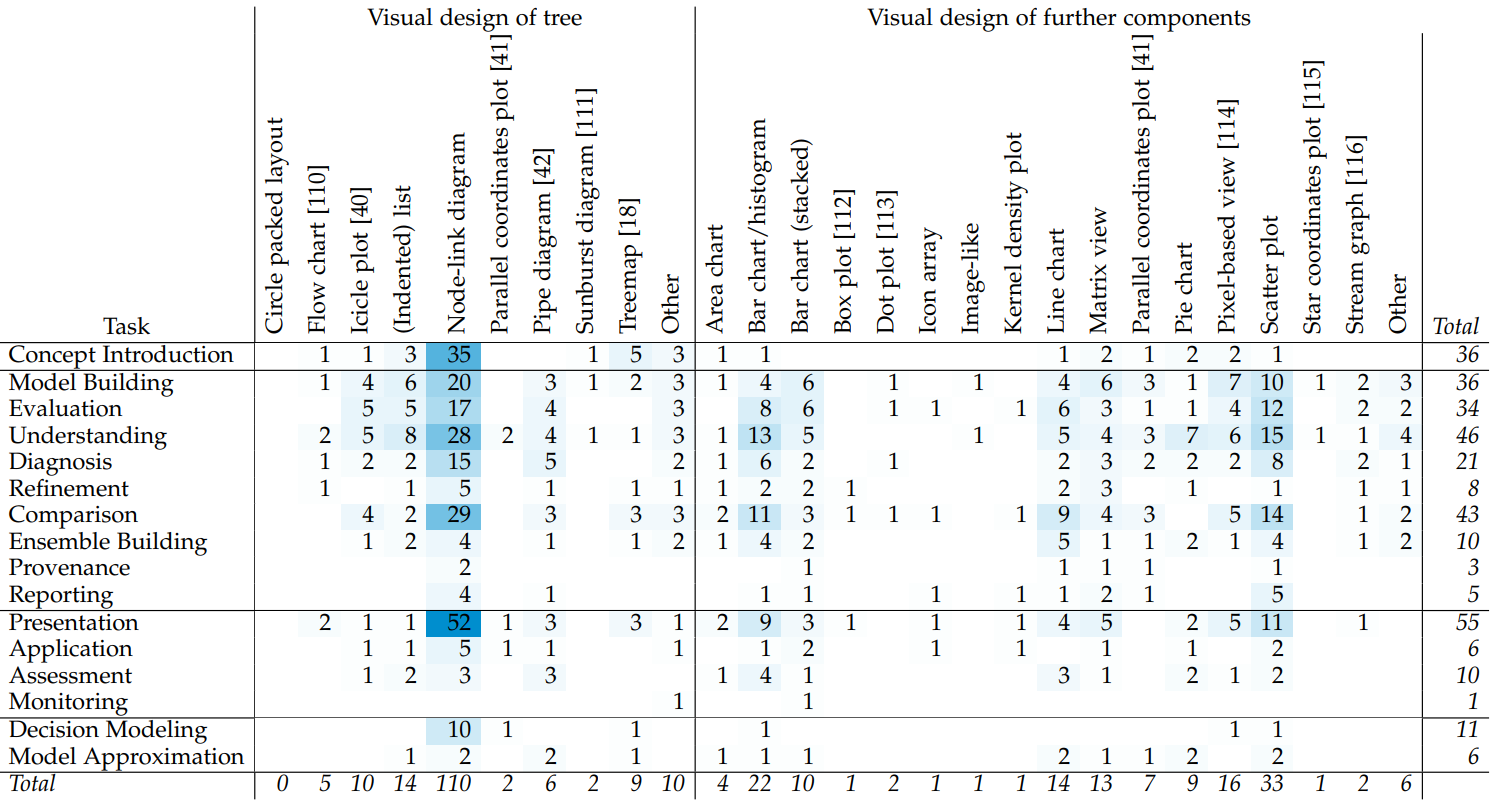
\includegraphics[width=\linewidth]{images/VisualDesignsOfTreesANDFurtherComponentsStreeb2021TaskBasedVI.png}
\end{table}

\paragraph{Traditional Layout Approaches}

The most fundamental category is classical tree layout algorithms. Hans-Jorg Schulz et al. \cite{schulz2011treevis} identify several core approaches including \textbf{node-link diagrams}, which represent the standard hierarchical visualization with explicit connections between parent and child nodes. The evolution of radial tree visualization approaches is particularly well-documented, as shown in Figure \ref{fig:radial_evolution}, which traces the development from natural patterns to interactive systems.

% Source: Treevis.net A Tree Visualization Reference, Page: 14, Figure 1
\begin{figure}[p]
    \centering
    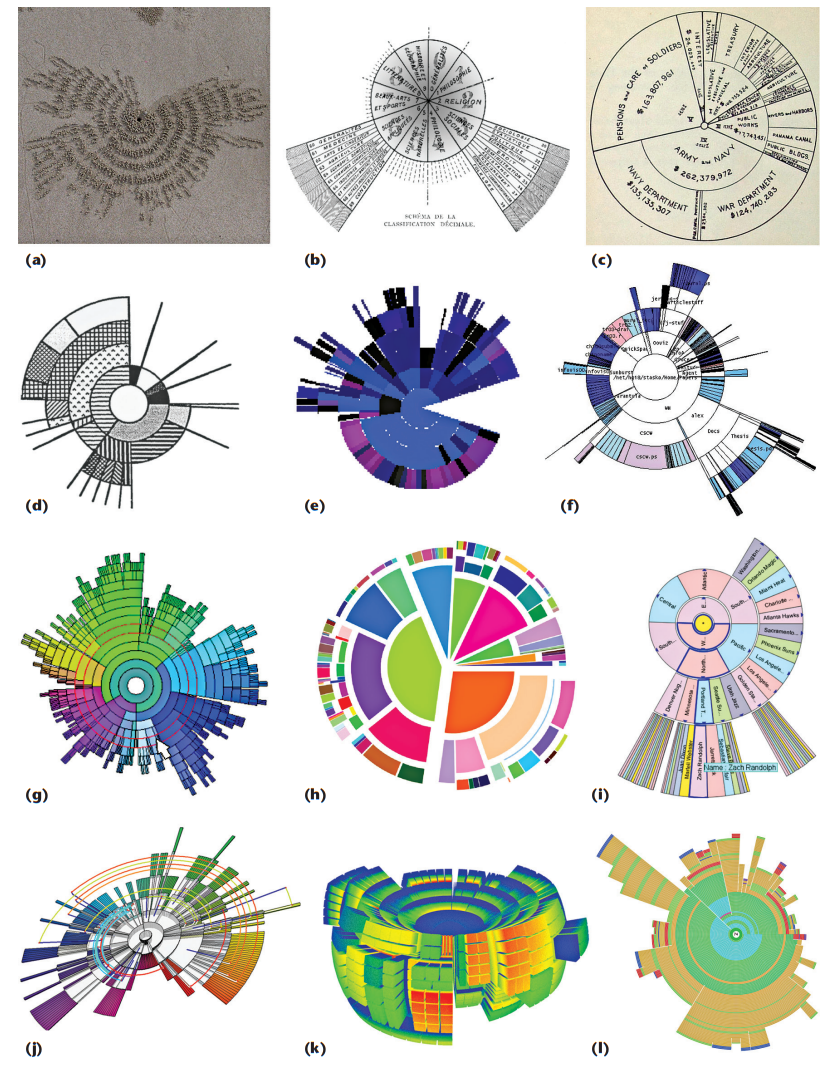
\includegraphics[width=0.85\linewidth]{images/treevis1.png}
    \caption{The evolution of radially stacked tree visualization. (a) Sand bubbler crab pattern (jkr1812 via Flickr).
(b) Universal decimal classification (1905, P. Otlet). (c) Hierarchical sector chart (1921, Am. Soc. Mechanical
Engineers). (d) Spoked polar tree map (1993, B. Johnson). (e) Aggregate tree map (1998, M. Chua). (f) Sunburst
(2000, J. Stasko). (g) Interring (2002, J. Yang et al.). (h) PieTree (2006, R. O’Donnell et al.). (i) FanLens (2008,
X. Lou et al.). (j) Enhanced radial space-filling layout (2009, M. Jia et al.). (k) 3D sunburst wheel (2010, H.-J.
Schulz and S. Hadlak). (l) Trevis calling-context tree ring chart (2010, A. Adamoli and M. Hauswirth). The
fundamental radial design turns out to be much older than most people think.}
    \label{fig:radial_evolution}
\end{figure}

\textbf{Indentation diagrams} provide a text-based alternative where parent-child relationships are conveyed through spatial indentation, though these suffer from poor structural overview for large trees \cite{elzen2011baobabview}. 

\paragraph{Coordinate-Based Visualizations}

A significant body of work explores coordinate system transformations for decision tree representation. Kovalerchuk et al. \cite{kovalerchuk2019interactive} introduce \textbf{General Line Coordinates (GLC)} with two variants: \textbf{Bended Coordinates (BC)} that bend at threshold points, and \textbf{Shifted Paired Coordinates (SPC)} that visualize n-dimensional points as directed graphs in 2D Cartesian coordinates.

\textbf{Parallel coordinates} integration has been explored by multiple researchers \cite{elzen2011baobabview, 10.1007/978-3-540-74205-0_121}, with noting attempts to combine decision trees with parallel coordinate plots, though these suffer from unclear class distribution representation. \textbf{Star coordinate plots} have been employed for interactive tree construction, allowing users to paint areas and assign class labels \cite{elzen2011baobabview, 10.1145/956750.956837, Teoh2003StarClassIV}. The StarClass/PaintingClass system workflow is illustrated in Figure \ref{fig:starclass_workflow}, demonstrating the integration of coordinate-based visualization with interactive model building.

% Source: TaskBased Visual Interactive Modeling Decision Trees and RuleBased Classifiers, Page: Figure 7
\begin{figure}[!htb]
    \centering
    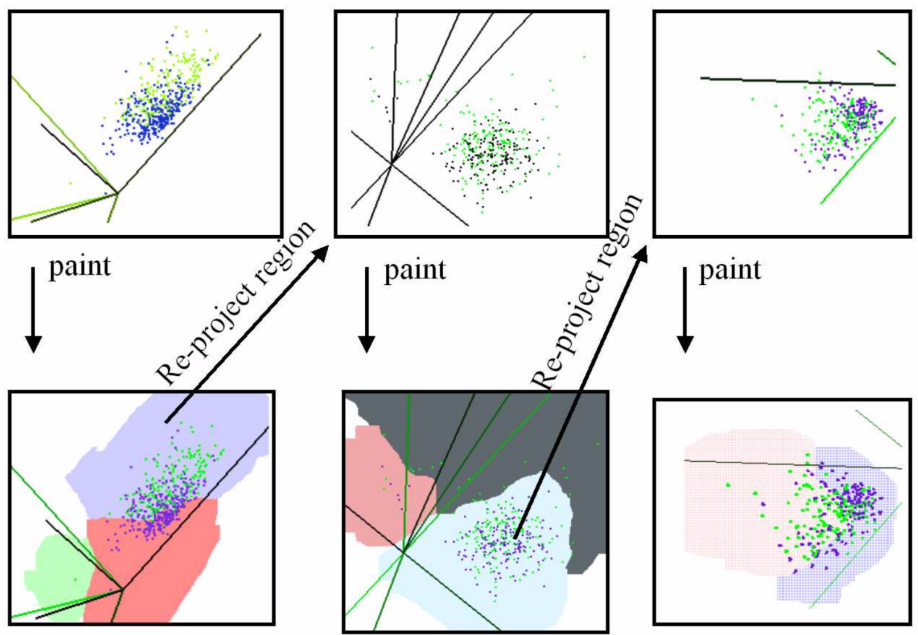
\includegraphics[width=0.9\linewidth]{images/starclass1.png}
    \caption{Workflow and visualization of the StarClass/PaintingClass system \cite{10.1007/978-3-540-74205-0_121, 10.1145/956750.956837}. During model building, analysts use re-projection and painting of regions at different levels of the hierarchy to effectively partition classes in the instance space. The system enables interactive decision boundary creation through direct manipulation of star coordinate projections.}
    \label{fig:starclass_workflow}
\end{figure}

\paragraph{Rule-Based and Matrix Visualizations}

Ming et al. \cite{ming2019rulematrix} pioneered the \textbf{matrix-based visualization} approach, where each row represents a decision rule and each column represents a feature. This technique transforms decision trees into a standardized rule-based knowledge representation, as illustrated in Figure \ref{fig:rulematrix_pipeline}, complemented by \textbf{stream plots} for continuous features and \textbf{stacked bar charts} for categorical features.
One can observe the resulting interface in Figure \ref{fig:rulematrix_interface}.

% Source: TaskBased Visual Interactive Modeling Decision Trees and RuleBased Classifiers, Page: Figure 2
\begin{figure}[!htb]
    \centering
    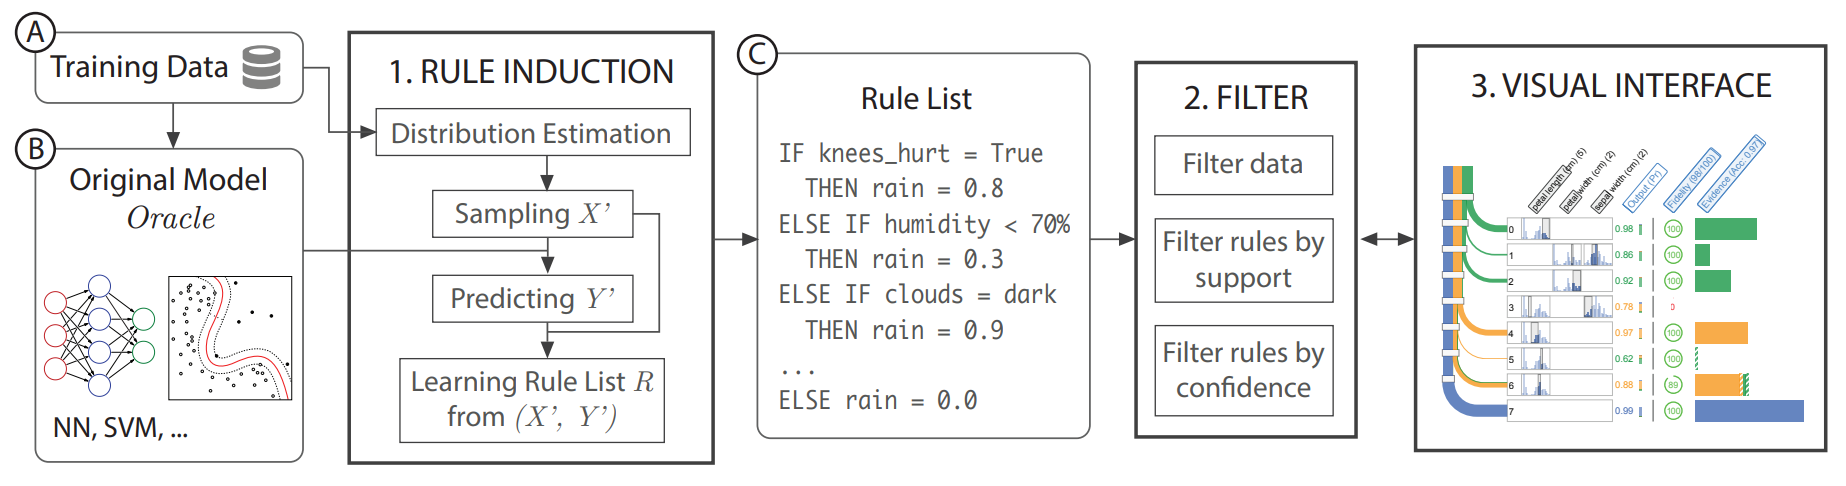
\includegraphics[width=0.9\linewidth]{images/rulematrix1.png}
    \caption{The pipeline for creating a rule-based explanation interface. The rule induction step (1) takes (A) the training data and (B) the model to be
explained as input, and produces (C) a rule list that approximates the original model. Then the rule list is filtered (2) according to user-specified
thresholds of support and confidence. The rule list is visualized as RuleMatrix (3) to help users navigate and analyze the rules.}
    \label{fig:rulematrix_pipeline}
\end{figure}

\begin{figure}[!htb]
    \centering
    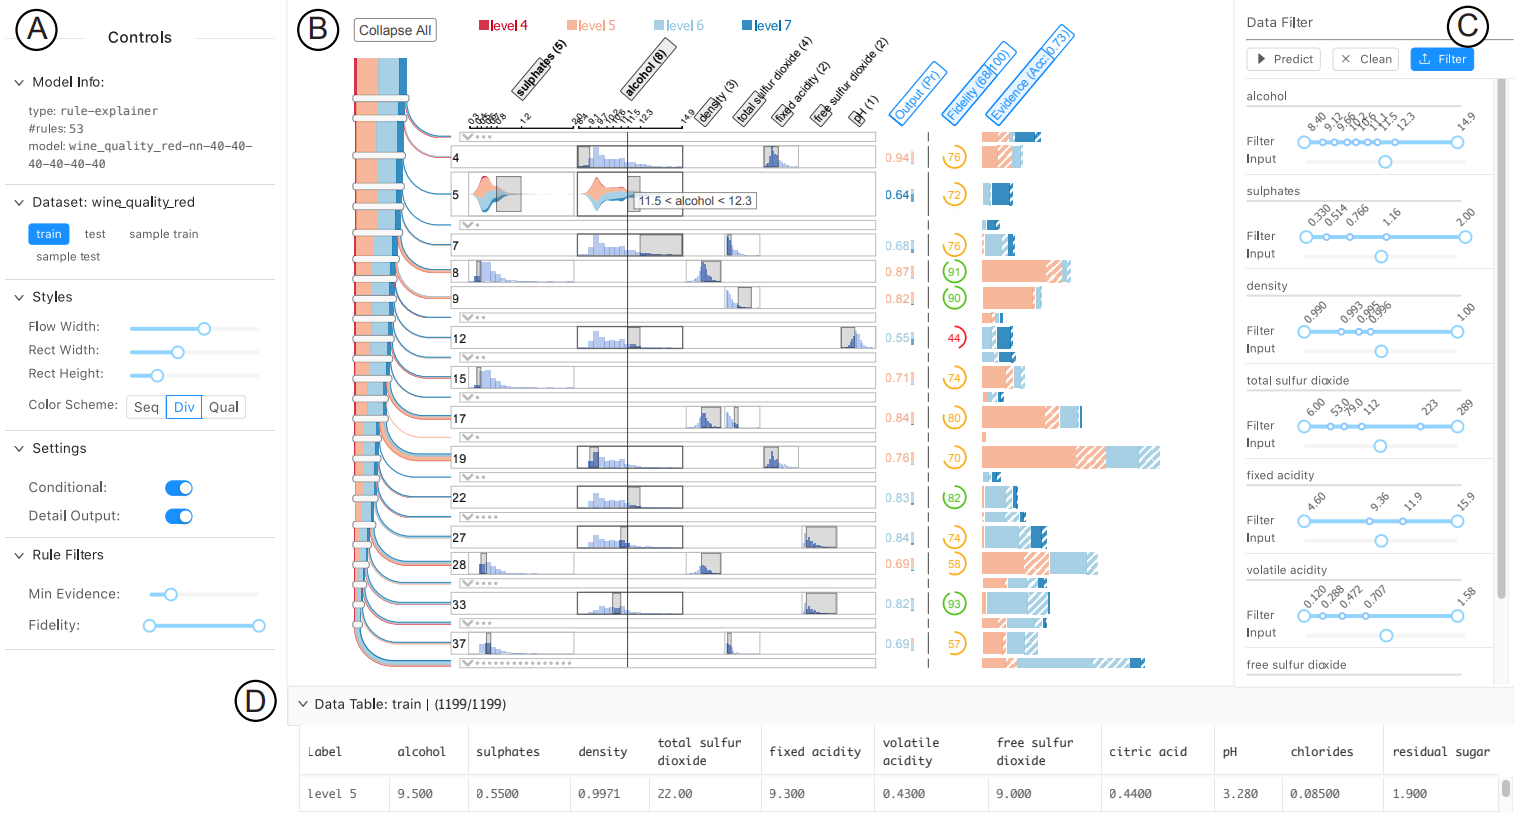
\includegraphics[width=\linewidth]{images/rulematrix2.png}
    \caption{ Understanding the behavior of a trained neural network using the explanatory visual interface of our proposed technique. The
user uses the control panel (A) to specify the detail information to visualize (e.g., level of detail, rule filters). The rule-based explanatory
representation is visualized as a matrix (B), where each row represents a rule, and each column is a feature used in the rules. The
user can also filter the data or use a customized input in the data filter (C) and navigate the filtered dataset in the data table (D).}
    \label{fig:rulematrix_interface}
\end{figure}

\paragraph{3D and Immersive Approaches}

Three-dimensional visualization techniques have been explored for enhanced spatial understanding. Mrva et al. \cite{mrva2019decision} present a \textbf{3D circular plane layout} where nodes are positioned based on depth from the root, with \textbf{3D bar charts} and \textbf{3D histograms} showing class distributions and feature relationships. This approach particularly emphasizes the visualization of attribute correlations beyond the primary splitting criterion, as shown in Figure \ref{fig:3d_medical_trees}.

\paragraph{Interactive and Advanced Visualization Systems}

Several comprehensive systems integrate multiple visualization techniques with interactability. \textbf{BaobabView} \cite{elzen2011baobabview} combines traditional node-link diagrams with integrated confusion matrices, attribute views, and data tables, emphasizing tight integration of visualization, interaction, and algorithmic support. The system's algorithmic support capabilities are detailed in Figure \ref{fig:baobab_algorithmic_support}, which shows how the interface provides visual guidance for split attribute selection.

% Source: TaskBased Visual Interactive Modeling Decision Trees and RuleBased Classifiers, Page: Figure 8
\begin{figure}[!htb]
    \centering
    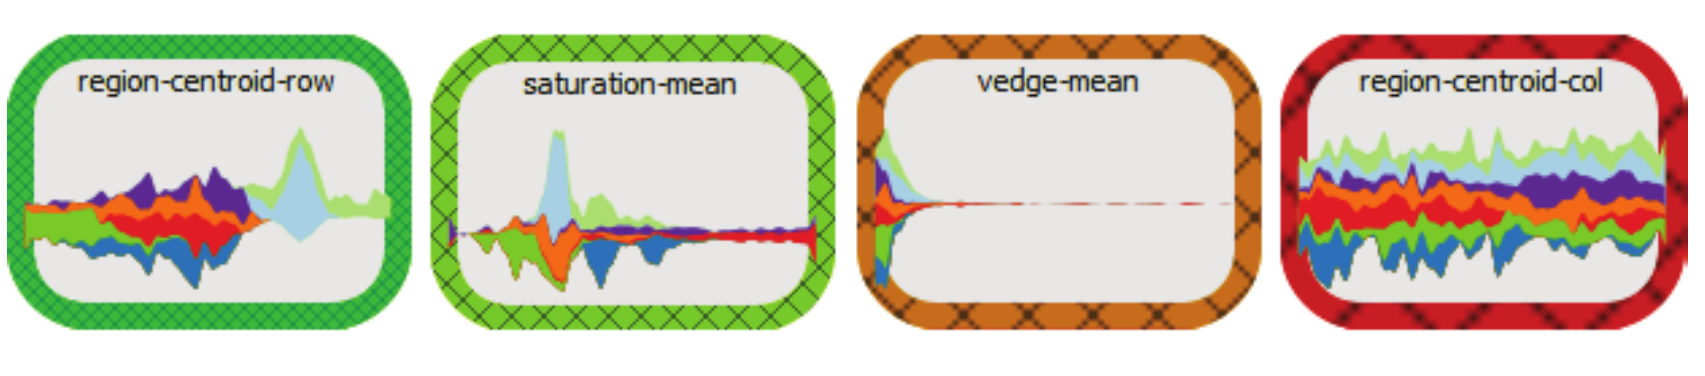
\includegraphics[width=0.8\linewidth]{images/Baobab2.png}
    \caption{The BaobabView system supports analysts with algorithmic support for selecting split attributes and presents suggestions visually. Border color indicates the goodness of the split as measured by the Gain-ratio, enabling users to make informed decisions about tree construction while maintaining control over the modeling process.}
    \label{fig:baobab_algorithmic_support}
\end{figure}

The data flow visualization capabilities of BaobabView are further illustrated in Figure \ref{fig:baobab_partitioning}, which shows how the system visualizes instance partitioning and highlights misclassifications.

% Source: TaskBased Visual Interactive Modeling Decision Trees and RuleBased Classifiers, Page: Figure 10
\begin{figure}[!htb]
    \centering
    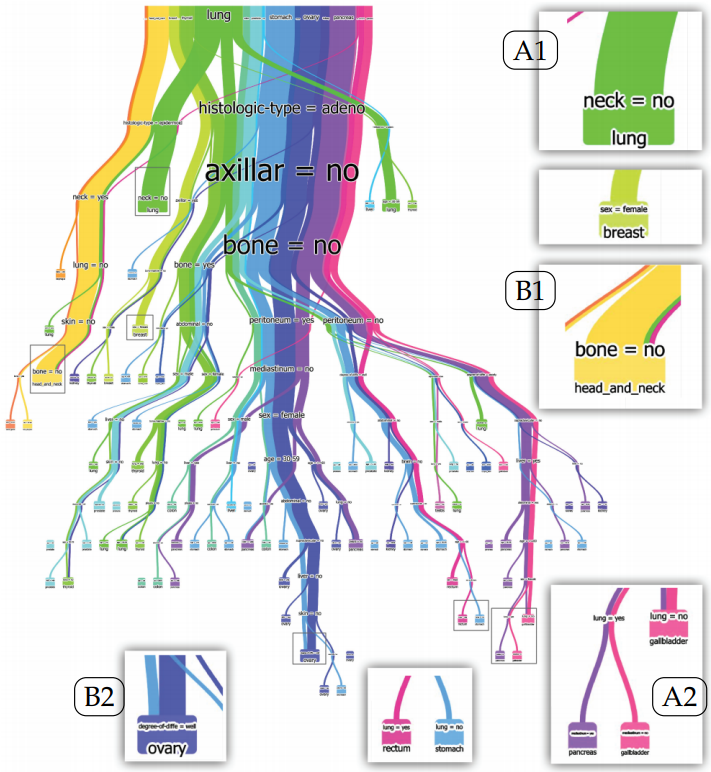
\includegraphics[width=0.8\linewidth]{images/Baobab3.png}
    \caption{BaobabView system showing the partitioning of instances.
Correct predictions are visible (A1, A2) and mis-classifications stand out
(B1, B2), enabling users to immediately identify areas where the decision tree performs poorly and may require refinement.}
    \label{fig:baobab_partitioning}
\end{figure}

\textbf{TIMBERTREK} \cite{wang2022timbertrek} introduces innovative \textbf{Sunburst diagrams} \cite{885091} for visualizing Rashomon sets of equally-performing decision trees, enabling users to explore thousands of model candidates through focus+context \cite{readingsInformationVi} interaction techniques, as demonstrated in Figure \ref{fig:timbertrek_system}.

\paragraph{Practical Tools and Libraries}

The landscape of practical implementations includes several notable tools. The \textbf{dtreeviz library} provides feature-target space visualization with \textbf{strip plots}, \textbf{scatter plots}, and decision boundary highlighting. Figure \ref{fig:tool_comparison} shows comprehensive comparisons between different tools from the library's authors' documentation on "how to visualize decision trees" \cite{parr2019dtreeviz}.

Standard machine learning libraries offer basic capabilities: \textbf{scikit-learn's plot\_tree}, \textbf{graphviz integration} for DOT format export, and \textbf{text-based representations} \cite{plonski2021visualize}. Specialized tools like the \textbf{supertree package} add interactive capabilities, including drag-and-zoom, node collapse/expand, and sample flow visualization between nodes \cite{plonski2021visualize}. Web-based implementations using \textbf{D3.js} enable interactive decision table to tree conversion and real-time traversal \cite{joesquito2024decision}.

% Source: webpage explained.ai decisiontreeviz, Multiple pages throughout document
\begin{figure}[p] 
    \centering
    \begin{subfigure}{0.5\textwidth}
        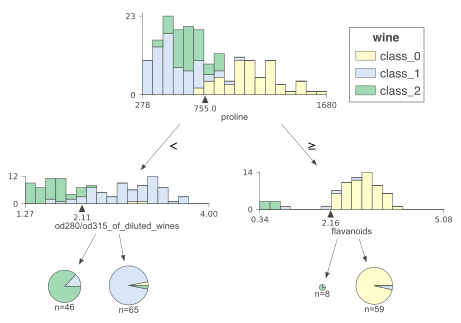
\includegraphics[width=\linewidth]{images/wine-TD-2.png}
        \caption{Wine 3-class top-down orientation}
        \label{fig:tool_comparison_wine-TD-2}
    \end{subfigure}\hfill
    \begin{subfigure}{0.5\textwidth}
        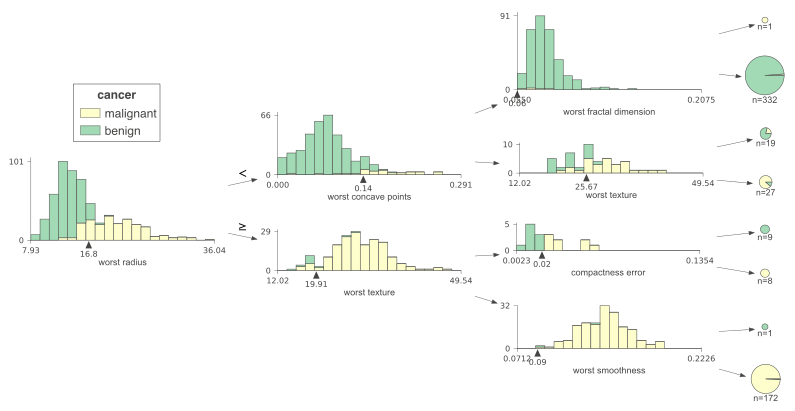
\includegraphics[width=\linewidth]{images/breast_cancer-LR-3.png}
        \caption{Breast cancer 2-class left-to-right}
        \label{fig:tool_comparison_breast_cancer-LR-3}
    \end{subfigure}
    \vspace{0.5cm} 
    \begin{subfigure}{0.48\textwidth}
        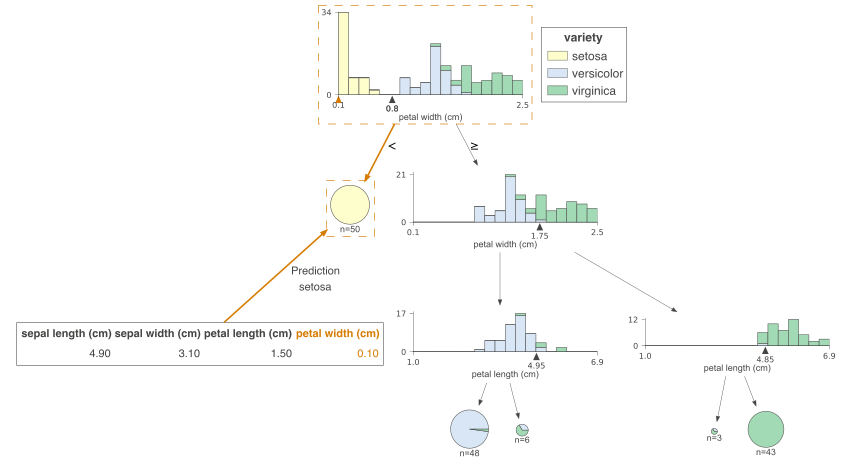
\includegraphics[width=\linewidth]{images/iris-TD-3-X.png}
        \caption{Iris 3-class showing a prediction}
        \label{fig:tool_comparison_iris-TD-3-X}
    \end{subfigure}\hfill
    \begin{subfigure}{0.48\textwidth}
        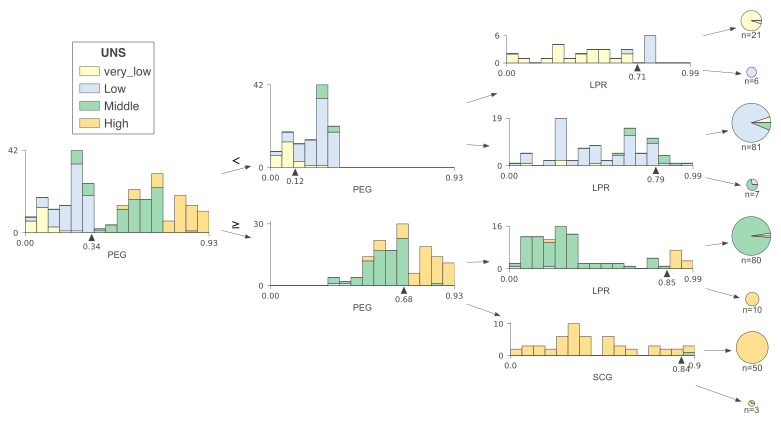
\includegraphics[width=\linewidth]{images/knowledge-LR-3.png}
        \caption{User knowledge rating 4-class}
        \label{fig:tool_comparison_knowledge-LR-3}
    \end{subfigure}
    \vspace{0.5cm}
    \begin{subfigure}{0.48\textwidth}
        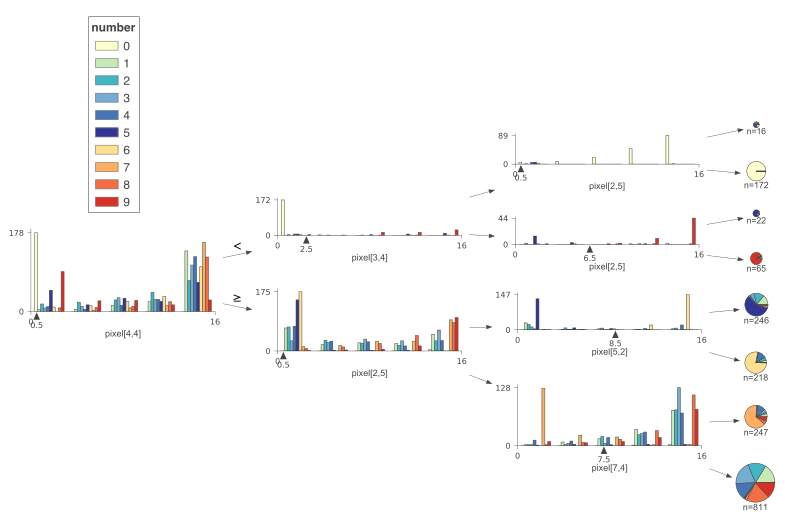
\includegraphics[width=\linewidth]{images/digits-LR-3.png}
        \caption{Digits 10-class}
        \label{fig:tool_comparison_digits-LR-3}
    \end{subfigure}\hfill
    \begin{subfigure}{0.48\textwidth}
        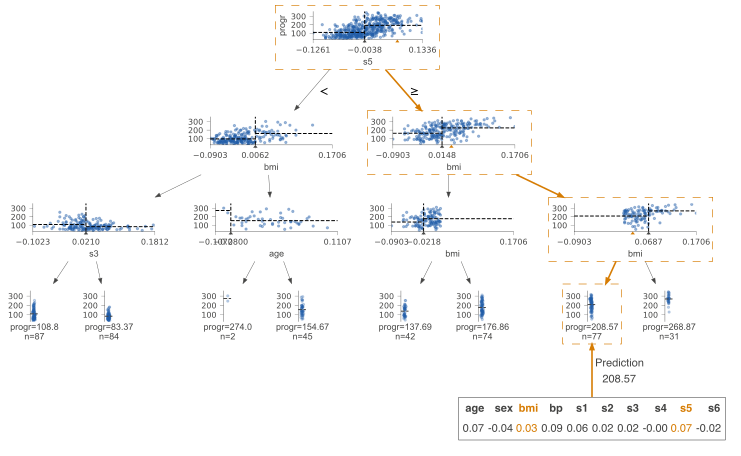
\includegraphics[width=\linewidth]{images/diabetes-TD-3-X.png}
        \caption{Diabetes showing a prediction}
        \label{fig:tool_comparison_diabetes-TD-3-X}
    \end{subfigure}
    \caption{Comprehensive comparison of decision tree visualization tools, including scikit-learn, dtreeviz, R packages, SAS, and IBM Watson. The comparison demonstrates how dtreeviz enhances traditional approaches by showing feature distributions as overlapping stacked histograms within decision nodes and using proportional leaf sizes, while maintaining clear decision boundary visualization.}
    \label{fig:tool_comparison}
\end{figure}

% Page 2 - Continuation of the same figure
\begin{figure}[p]
    \ContinuedFloat  % This keeps the same figure number
    \centering
        
    \begin{subfigure}{0.48\textwidth}
        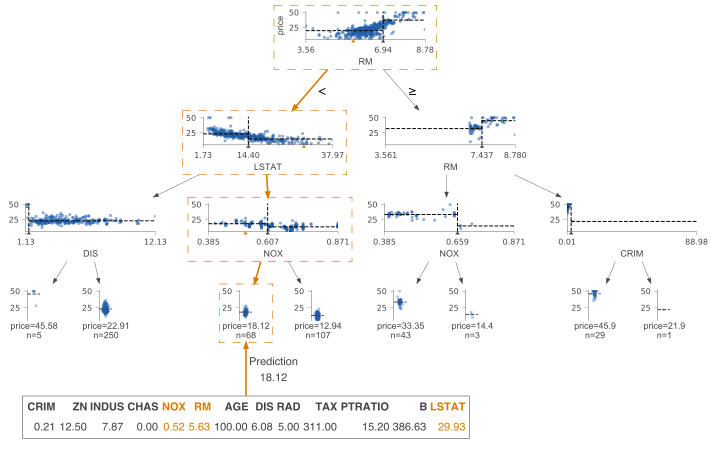
\includegraphics[width=\linewidth]{images/boston-TD-3-X.png}
        \caption{Boston showing a prediction}
        \label{fig:tool_comparison_boston-TD-3-X}
    \end{subfigure}\hfill
    \begin{subfigure}{0.48\textwidth}
        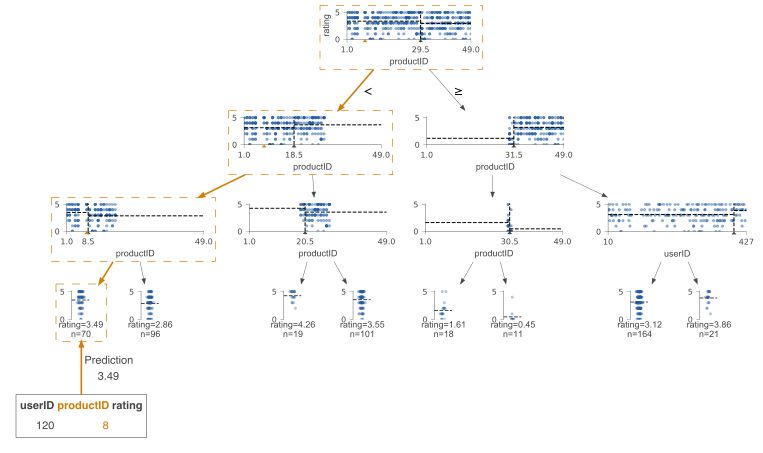
\includegraphics[width=\linewidth]{images/sweets-TD-3-X.png}
        \caption{Sweets showing a prediction}
        \label{fig:tool_comparison_sweets-TD-3-X}
    \end{subfigure}
    \vspace{0.5cm}
    
    \begin{subfigure}{0.48\textwidth}
        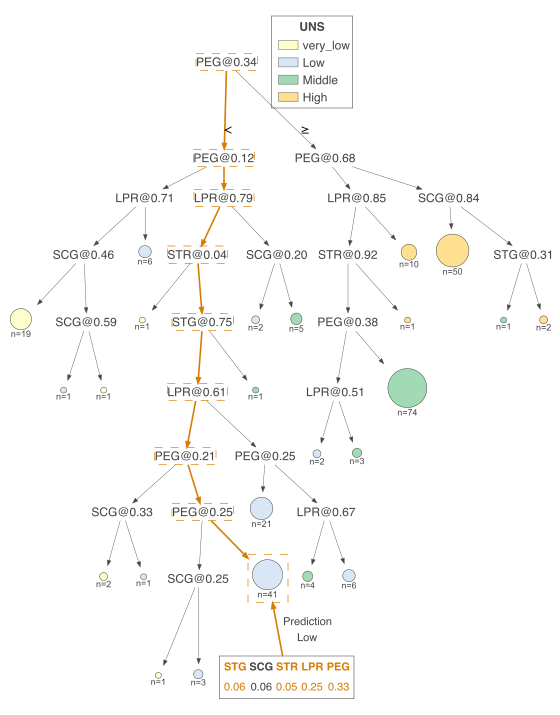
\includegraphics[width=\linewidth]{images/knowledge-TD-15-X-simple.png}
        \caption{User knowledge rating 4-class non-fancy}
        \label{fig:tool_comparison_knowledge-TD-15-X-simple}
    \end{subfigure}\hfill
    \begin{subfigure}{0.48\textwidth}
        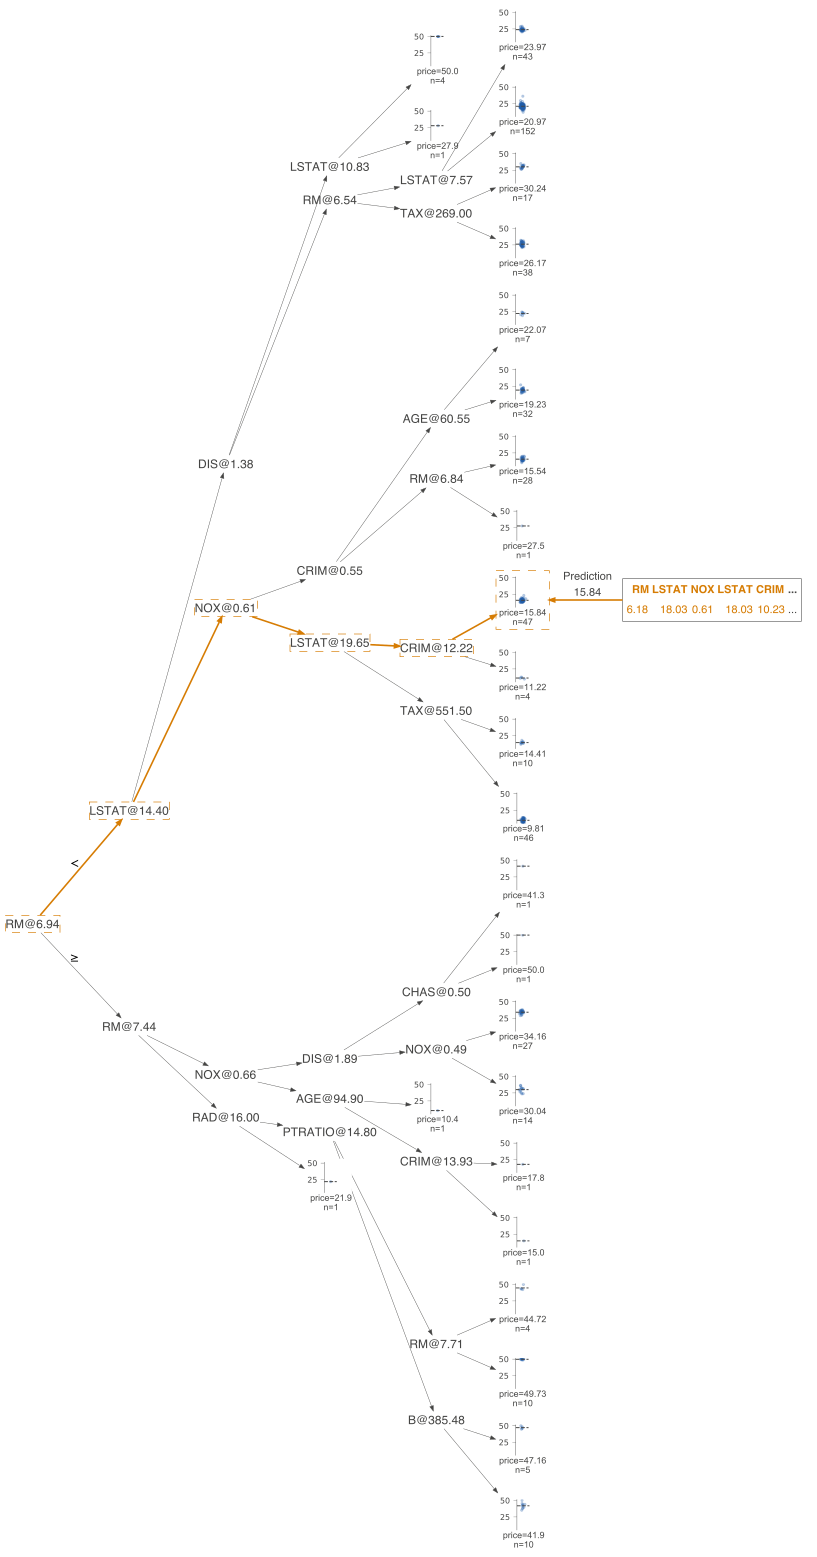
\includegraphics[width=\linewidth]{images/boston-LR-5-X-simple.png}
        \caption{Diabetes non-fancy}
        \label{fig:tool_comparison_boston-LR-5-X-simple}
    \end{subfigure}
    \caption*{Figure \ref{fig:tool_comparison} (continued)}
\end{figure}

\paragraph{Hybrid and Multi-View Approaches}

An emerging trend involves the combination of multiple visualization paradigms within unified interfaces. Van den Elzen et al. \cite{elzen2011baobabview} demonstrate the integration of tree structure visualization with data distribution views, confusion matrices, and alternative dataset exploration. Similarly, Fisher et al. \cite{fisher2012making} discuss the broader principles of coordinated multiple views, including overview and detail patterns and multiform visualizations that could be applied to decision tree contexts.

This comprehensive landscape reveals both the richness of available techniques and the fragmentation of approaches, with limited systematic evaluation of when different visualization paradigms are most effective for specific interpretability goals.

\subsubsection{Visualization Design Patterns in Decision Tree Literature}

The comprehensive analysis by Streeb et al. \cite{Streeb2021TaskBasedVI} reveals clear patterns in how decision trees are visualized across 152 publications. Their systematic categorization, presented in Tables \ref{tab:VisualDesignsOfTreesANDFurtherComponentsStreeb2021TaskBasedVI} and \ref{tab:measureStreeb2021TaskBasedVI}, demonstrates the dominance of certain approaches in current practice.

\paragraph{Visual Design Preferences}
The survey reveals a strong preference for traditional node-link diagrams, which appear in 110 of the 152 publications, making them by far the most common approach to representing tree structure. Other tree visualization techniques show much lower adoption rates: treemaps appear in only 9 publications, icicle plots in 10, and pipe diagrams in 6. This concentration suggests that despite advances in hierarchical visualization techniques, the research community largely agrees on the fact that conventional tree representations are more effective.

For additional visual components beyond the core tree structure, the analysis shows frequent use of standard statistical visualizations. Bar charts and histograms appear in more than 20 publications, line charts in almost 15, and scatter plots in more than 30. These findings indicate that researchers commonly augment tree visualizations with familiar chart types.

% % Not relevant to the current analysis
% \paragraph{Quality Measure Integration}
% Perhaps most relevant is the limited integration of quality measures in tree visualizations. Table \ref{tab:measureStreeb2021TaskBasedVI} reveals that only 79 of the 152 publications display any quality measures at all. Among those that do, accuracy dominates with more than 25 appearances, while other important measures like precision, recall, F1-score and $\chi^2$ appear in fewer than 5 publications each. This pattern suggests a significant missed opportunity for helping users understand model performance through visual means.

\paragraph{Node Design and Encoding Strategies}

% \textbf{Size Encoding for Sample Representation:} 
A consistent pattern across multiple systems involves encoding sample sizes through node dimensions. Wang et al. \cite{wang2022timbertrek} demonstrate \textbf{funnel-like node representations} where node width corresponds to the percentage of training samples, enabling users to quickly identify important decision points and assess model robustness. Similarly, Wang et al. \cite{wang2022timbertrek} employ node size variations to represent the significance of different tree components within the Rashomon set \cite{Streeb2021TaskBasedVI}.

% \textbf{Multi-layered Node Content:} 
Effective node design integrates multiple information layers without overwhelming users. Elzen et al. \cite{elzen2011baobabview} showcase nodes containing \textbf{class distributions via streamgraphs}, \textbf{attribute values}, and \textbf{split conditions}, all within compact visual representations, as demonstrated in Figure \ref{fig:baobab_interface}. Ming et al. \cite{ming2019rulematrix} demonstrate how \textbf{compact clause representations} can be combined with \textbf{data distribution previews} using histograms for continuous features and bar charts for categorical features.

% % Not relevant to the current analysis
% \textbf{Performance Indicators:} Visual encoding of prediction confidence and accuracy represents a critical best practice. Wang et al. \cite{wang2022timbertrek} use \textbf{opacity encoding for leaf node accuracy}, allowing users to quickly assess prediction confidence across the tree. Ming et al. \cite{ming2019rulematrix} integrate \textbf{evidence bars} and \textbf{fidelity metrics} directly into the node representation, providing immediate feedback on rule quality.

\paragraph{Color Coding Strategies and Accessibility}

% \textbf{Class-Based Color Schemes:} 
Consistent color coding for target classes emerges as a fundamental pattern. Parr et al. \cite{parr2019dtreeviz} emphasize the use of \textbf{handpicked colorblind-safe palettes}, with distinct schemes for different numbers of target categories (2 through 10). This approach ensures accessibility while maintaining visual coherence across complex trees.

% \textbf{Attribute and Feature Highlighting:} 
Several systems employ color to highlight important features and decision paths. Elzen et al. \cite{elzen2011baobabview} use \textbf{attribute-based node coloring} to reveal which features are most frequently used in splitting decisions. Parr et al. \cite{parr2019dtreeviz} use \textbf{orange wedge highlighting} for decision paths, making the comparison operations easily visible during tree traversal.

% \textbf{Gradient and Transparency Techniques:} 
Advanced color strategies include the use of transparency and gradients to convey additional information layers. Ming et al. \cite{ming2019rulematrix} employ \textbf{higher opacity for satisfied conditions} and \textbf{gradient coloring for confidence intervals}. Mrva et al. \cite{mrva2019decision} use \textbf{transparent rendering for filtered nodes}, allowing users to focus on specific classes while maintaining context.

\paragraph{Edge Representation and Data Flow Visualization}

% \textbf{Variable Width Edges:} 
A recurring best practice involves encoding data flow through edge thickness. Elzen et al. \cite{elzen2011baobabview} pioneer the use of \textbf{color-banded edges with variable width} to visualize the volume of data flowing through each decision branch. This technique provides immediate visual feedback about data distribution across the tree structure, as demonstrated in Figure \ref{fig:baobab_partitioning}.

% \textbf{Decision Path Highlighting:}
Multiple systems implement strategies for highlighting active decision paths. Parr et al. \cite{parr2019dtreeviz} use \textbf{thicker, colored edges} for paths involved in specific predictions, while Joesquito \cite{joesquito2024decision} employs \textbf{animated traversal} with color transitions to show decision progression in real-time.

% \textbf{Label Positioning and Clarity:} 
Consistent edge labeling practices include positioning Y/N or condition labels at strategic points along edges. Joesquito \cite{joesquito2024decision} demonstrates optimal \textbf{midpoint label placement} with appropriate spacing from both source and target nodes.

\paragraph{Layout and Spatial Organization}

% \textbf{Hierarchical Consistency:} 
Maintaining consistent spatial relationships across tree levels represents a fundamental design principle. Schulz et al. \cite{schulz2011treevis} identify \textbf{layer-based organization} as essential for preserving tree topology understanding. Elzen et al. \cite{elzen2011baobabview} implement \textbf{weighted edge algorithms} that optimize readability while minimizing edge crossings.

% \textbf{Adaptive Layouts:} 
Advanced systems implement layout algorithms that adapt to tree characteristics. Wang et al. \cite{wang2022timbertrek} introduce \textbf{focus+context techniques} \cite{readingsInformationVi} using Sunburst diagrams \cite{885091} that allow seamless transitions between overview and detail levels.

\paragraph{Integration of Data Distributions}

% \textbf{Feature-Target Space Visualization:} 
One of the best practices found involves directly integrating data distribution information within tree visualizations. Parr et al. \cite{parr2019dtreeviz} demonstrate the effectiveness of \textbf{strip plots and scatter plots} embedded within decision nodes, showing actual data distributions for split conditions, as illustrated in Figure \ref{fig:tool_comparison}. This approach eliminates the cognitive burden of connecting abstract tree structure with the underlying data patterns.

% \textbf{Contextual Distribution Views:} 
Ming et al. \cite{ming2019rulematrix} implements \textbf{conditional distribution visualization} that shows feature distributions given that previous rules are not satisfied, providing crucial context for understanding rule interactions. Mrva et al. \cite{mrva2019decision} extend this concept with \textbf{3D histograms} comparing parent and child node distributions, as shown in Figure \ref{fig:3d_medical_trees}.

\paragraph{Interaction Design Patterns}

% \textbf{Progressive Disclosure:} 
Effective interaction design balances information density with usability through progressive disclosure mechanisms. Ming et al. \cite{ming2019rulematrix} implement \textbf{details-on-demand} through hover interactions and expandable cells, while Wang et al. \cite{wang2022timbertrek} provide \textbf{repositionable tree windows} for comparative analysis, as demonstrated in Figure \ref{fig:timbertrek_system}.

% \textbf{Dynamic Filtering and Exploration:} 
Multiple systems implement sophisticated filtering capabilities. Ming et al. \cite{ming2019rulematrix} provide \textbf{rule filtering by support and confidence}, while Mrva et al. \cite{mrva2019decision} enable \textbf{class-based filtering} with transparency adjustments. Elzen et al. \cite{elzen2011baobabview} demonstrate \textbf{real-time threshold modification} with immediate visual feedback, as shown in Figure \ref{fig:baobab_algorithmic_support}.

% \textbf{Coordinated Multiple Views:} 
Advanced systems integrate tree visualization with complementary views. Elzen et al. \cite{elzen2011baobabview, 10.5555/383784} coordinate tree views with \textbf{confusion matrices}, \textbf{attribute distributions}, and \textbf{alternative dataset views}, as demonstrated in Figure \ref{fig:baobab_interface}. Fisher et al. \cite{fisher2012making} establish theoretical foundations for such coordination through \textbf{brushing and linking} techniques.

\paragraph{Typography and Readability}

% \textbf{Readable Text Design:} 
Subtle but important patterns emerge in text presentation. Parr et al. \cite{parr2019dtreeviz} advocate for \textbf{gray rather than black text} to reduce eye strain, while maintaining sufficient contrast for accessibility. \textbf{Hairline borders} and \textbf{outlined shapes} improve element separation without overwhelming visual complexity.

% \textbf{Hierarchical Information Architecture:} 
Effective systems organize textual information hierarchically within nodes. Ming et al. \cite{ming2019rulematrix} demonstrate \textbf{matrix organization} where feature order remains consistent across rules, facilitating rapid visual comparison and rule understanding, as illustrated in Figure \ref{fig:rulematrix_pipeline}.

These patterns collectively establish a foundation for effective surrogate models visualization, emphasizing the importance of integrating multiple information dimensions while maintaining visual clarity and supporting diverse interaction paradigms. 
The latter analysis of various pieces of literature provides a comprehensive framework for future decision tree visualization development, highlighting both well-established practices and emerging innovative approaches that push the boundaries of traditional tree representation techniques.

        \subsection{Existing XAI Visual Analytics Tools}
        

The escalation of complex machine learning models across various domains has prompted the development of visual analytics tools designed to make these models more interpretable and trustworthy. While the theoretical foundations of eXplainable Artificial Intelligence have been extensively studied, the practical implementation of these concepts through interactive visual systems represents a critical need to connect the algorithmic explanations to human understanding \cite{8807299,analytics4010007}.

As highlighted by Spinner et al.\cite{8807299}, there exists a significant gap between theoretical XAI frameworks and their use in practical systems that support real-world model development and deployment workflows. This gap becomes particularly pronounced when considering the diverse user groups that interact with machine learning models, from domain experts with limited technical background to experienced data scientists in need of algorithmic insights \cite{Z_ller_2023}.

The landscape of XAI visual analytics tools has evolved to address different aspects of the explainability challenge, ranging from comprehensive frameworks that integrate multiple explanation methods \cite{8807299} to specialized tools that focus on specific explanation paradigms such as local explanations \cite{9861728,cappuccio2024fipervisualbasedexplanationcombining} or surrogate model visualization \cite{Chatzimparmpas2023DeforestVisBA}. However, most existing approaches tend to address either global model understanding or local instance explanations, and in the latter case, they rarely provide integrated views that make the relationship between the generated neighborhood and the resulting explanation obvious.

In the context of this thesis, which focuses on developing an interactive explanation system for 
% the $\text{LORE}_{sa}$ algorithm
explainability methods which involve both a synthetically generated neighborhood and a surrogate model, 
understanding the current state of visual eXplainable Artificial Intelligence tools is crucial. The integration of dimensionality reduction techniques (such as UMAP projections) with decision tree visualization presents specific design challenges that few existing tools have addressed.

This section examines the current state of the art of XAI visual analytics tools, organizing them into several categories based on their primary focus and methodological approach. We analyze comprehensive frameworks that attempt to unify multiple XAI methods \cite{8807299,Z_ller_2023}, specialized tools for local explanation analysis \cite{9861728,cappuccio2024fipervisualbasedexplanationcombining}, surrogate model visualization approaches \cite{Chatzimparmpas2023DeforestVisBA}, and industrial deployment considerations \cite{analytics4010007}.

Through this analysis, we identify key design patterns, interaction paradigms, and visualization techniques that inform the development of effective interfaces.
% for $\text{LORE}_{sa}$ explanations. 
Particular attention is paid to tools that employ scatter plot visualizations for neighborhood representation and surrogate model interfaces for rule exploration, as these components are central to the proposed system. Furthermore, we examine how existing tools handle the coordination between different explanation views and support user interaction workflows that allow both exploratory analysis and targeted explanation refinement.

\subsubsection{Comprehensive XAI Visual Analytics Frameworks}

Comprehensive XAI visual analytics frameworks represent an ambitious approach to addressing the XAI field. Unlike specialized tools that focus on particular explanation methods or user scenarios, comprehensive frameworks attempt to integrate multiple XAI techniques within unified platforms that support diverse workflows and user needs. Two notable examples are \textbf{explAIner} and \textbf{XAutoML}, each addressing different aspects of the machine learning lifecycle while providing comprehensive approaches to model understanding and confirmation.

\paragraph{explAIner: Interactive Deep Learning Model Analysis}

This 
% \textbf{explAIner} 
framework \cite{8807299} presents a complete approach to interactive and eXplainable Artificial Intelligence, specifically designed for deep learning models and integrated in the TensorBoard ecosystem. The framework is built around an iterative XAI pipeline that structures the explanation process into three core phases: \textit{understanding}, \textit{diagnosis}, and \textit{refinement}. 

The central concept in this framework are the \textit{explainers}, which serve as a modular building block that take one or more model states as input, applies an XAI method, and outputs either explanations (visualizations, verbalizations, surrogate models) or transition functions for model refinement. The framework distinguishes between single-model explainers that analyze individual model states and multi-model explainers that perform comparative analysis across different model configurations. This modular design enables the integration of diverse explanation methods including LIME \cite{ribeiro2016should}, LRP \cite{Bach2015OnPE}, SHAP \cite{lundberg2017unified}, gradient-based methods, and custom implementations.

\begin{figure}
    \centering
    \begin{subfigure}[c]{0.6\textwidth}
        \centering
        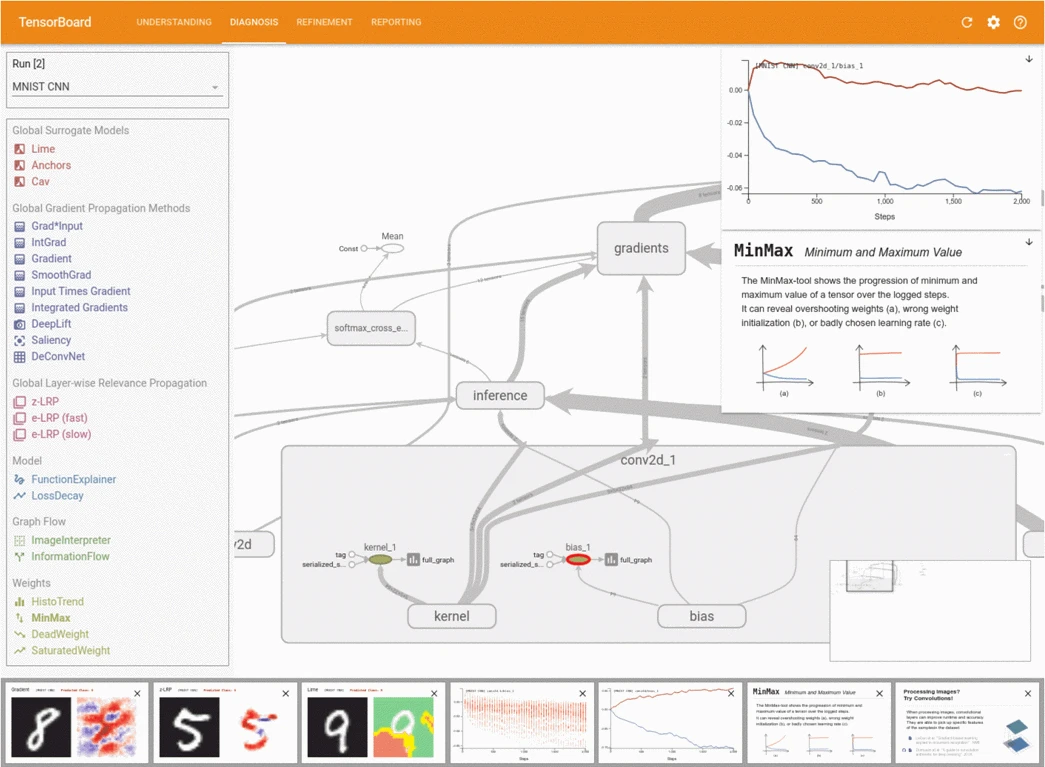
\includegraphics[width=\textwidth]{images/eXplainer dashboard.png}
        \caption{The diagnosis dashboard. Explainers are arranged in a
toolbox-like interface, ordered descending, from high-abstraction to
low-abstraction. The graph visualization provides an overview of the
full model and allows for node selection. Explanations are shown in
the upper toolcard, while information about the explainer is displayed
beneath. The provenance bar contains cards from interesting findings}
        \label{fig:eXplainer_dashboard}
    \end{subfigure}
    \hfill
    \begin{subfigure}[c]{0.39\textwidth}
        \centering
        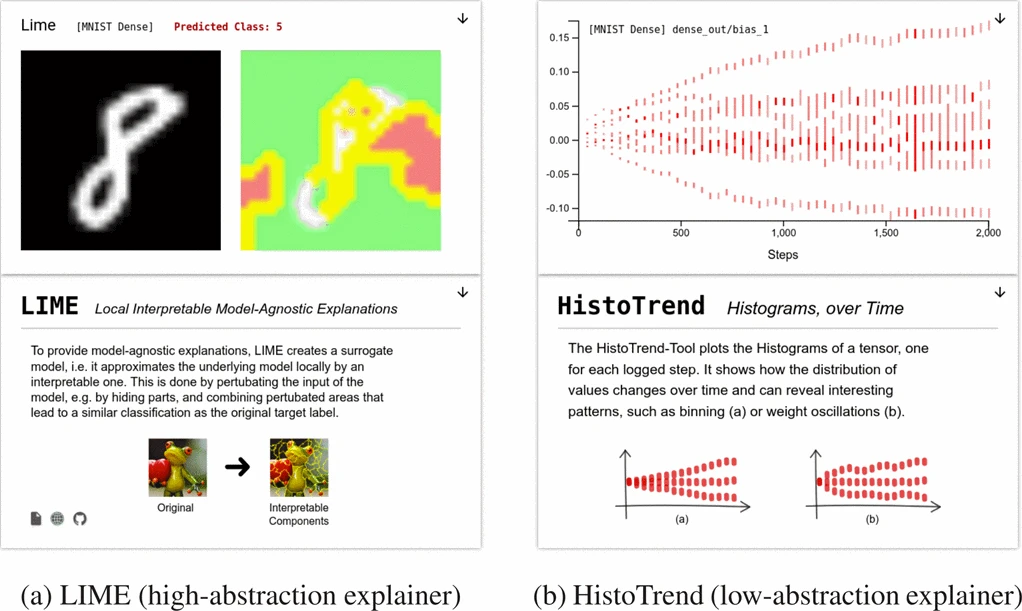
\includegraphics[width=\textwidth]{images/eXplainer card.png}
        \caption{Information cards showing results for different explainers (top)
with the corresponding descriptions for the explainer itself (bottom).}
        \label{fig:eXplainer_cards}
    \end{subfigure}
    \caption{eXplainer interface.}
    \label{fig:eXplainer}
\end{figure}

The framework incorporates eight global monitoring and steering mechanisms that support the overall explanation process, including model quality monitoring, search space exploration, data shift scoring, comparative analytics, provenance tracking, XAI Strategies, knowledge generation, and reporting capabilities. These mechanisms provide essential infrastructure for maintaining context and continuity across extended explanation sessions, allowing users to track their investigation process and build cumulative understanding over time.

From a visualization perspective, explAIner employs a toolbox-based interface, shown in Figure \ref{fig:eXplainer_dashboard}, where explainers are arranged by abstraction level, allowing users to progressively examine the results from high-level model understanding to detailed component analysis. The system's integration with TensorBoard's graph visualization provides a familiar foundation for users already working with deep learning models, while overlay cards, represented in Figure \ref{fig:eXplainer_cards}, present explanatory results and supplementary information based on context.

\paragraph{XAutoML: Transparency for Automated Machine Learning}

While explAIner focuses on manually developed deep learning models, \textbf{XAutoML} \cite{Z_ller_2023} addresses the understanding and of automated machine learning (AutoML) systems. 

% Source: XAutoML paper, page 15
\begin{figure}[ht!]
\centering
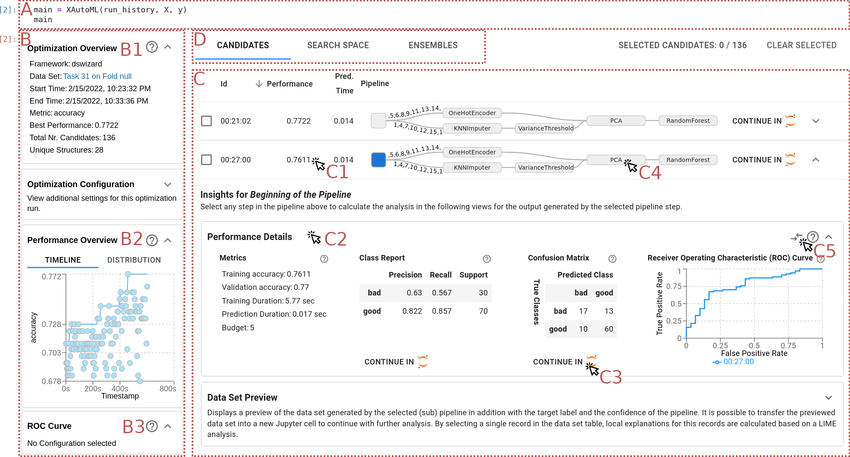
\includegraphics[width=\textwidth]{images/Overview-of-XAutoML-A-The-visualization-is-integrated-with-Jupyter-and-can-be-accessed.png}
\caption{Overview of XAutoML. The visualization is integrated with Jupyter and can be accessed with a few lines of code (A). On the
left side (B), the optimization overview provides basic statistics about the optimization run (B1), a scatter plot of the accuracy of all
candidates over time (B2), and a receiver operating characteristic (ROC) curve of selected candidates (B3, hidden). The leaderboard
view (C, partially hidden) provides a comprehensive overview of all evaluated candidates. Users can open single candidates (C1) in
an overlay on the right-hand side to reveal detailed information about them (only partially visible). The candidate details contain
various boxes grouping related information together. In the performance details view (C2), performance metrics and basic performance
visualizations are available. By clicking the Continue in Jupyter button (C3), the according information can be exported to a new
Jupyter cell. Users can access the search space and ensemble inspection via the tabs at the top (D).}

\label{fig:xautoml_overview}
\end{figure}

The widespread use of AutoML tools produced high-performing models that do not reveal the processes or design decisions behind the obtained pipelines.
XAutoML tackles this challenge through a comprehensive visual analytics approach embedded within JupyterLab, providing four primary views that cover different aspects of the AutoML process. As shown in Figure \ref{fig:xautoml_overview}, the \textit{optimization overview} provides high-level insights into the AutoML run, including performance trajectories over time, candidate distribution by performance, and ROC curve comparisons for selected models. The \textit{candidate inspection} view enables detailed analysis of individual ML pipelines, through XAI techniques such as surrogate models, feature importance analysis, and partial dependence plots.

% Source: XAutoML paper, page 16
\begin{figure*}[htbp]
    \centering
    
    \begin{subfigure}[t]{0.48\textwidth}
        \centering
        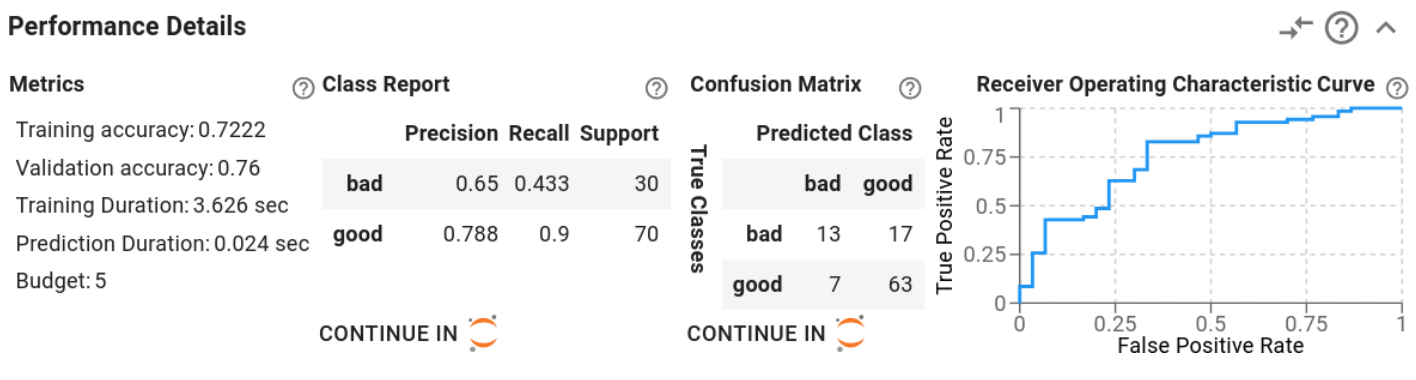
\includegraphics[width=\textwidth]{images/XAutoML a.png}
        \caption{Performance details. From left to right some basic metrics, a class report, a confusion matrix and a ROC curve is displayed.}
        \label{fig:performance_details}
    \end{subfigure}
    \hfill
    \begin{subfigure}[t]{0.48\textwidth}
        \centering
        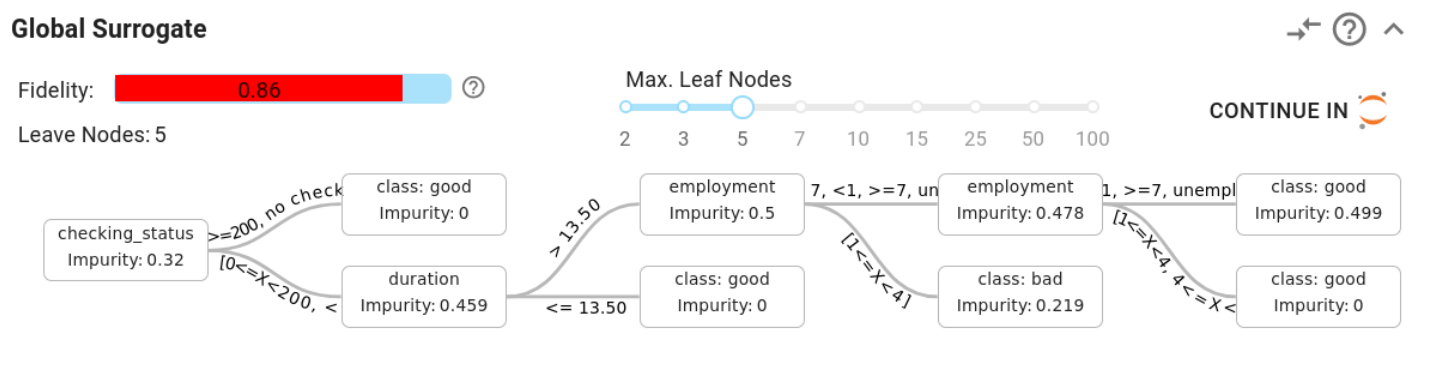
\includegraphics[width=\textwidth]{images/XAutoML b.png}
        \caption{Global surrogate. A decision tree is rendered as a global surrogate. Using the top slider, the tree complexity can be controlled.}
        \label{fig:global_surrogate}
    \end{subfigure}
    
    \vspace{0.5cm}
    
    \begin{subfigure}[t]{0.48\textwidth}
        \centering
        \includegraphics[width=\textwidth]{images/XAutoML c.png}
        \caption{Dataset preview and local surrogate. The left-hand side displays a preview of the input dataset. On the right-hand side feature attributions for the selected sample are displayed.}
        \label{fig:dataset_preview}
    \end{subfigure}
    \hfill
    \begin{subfigure}[t]{0.48\textwidth}
        \centering
        \includegraphics[width=\textwidth]{images/XAutoML d.png}
        \caption{Model details. At the top, the selected hyperparameter configuration is displayed in a CPC. At the bottom, the aggregated structure search graph up to this candidate is rendered.}
        \label{fig:model_details}
    \end{subfigure}
    
    \vspace{0.5cm}
    
    \begin{subfigure}[t]{0.48\textwidth}
        \centering
        \includegraphics[width=\textwidth]{images/XAutoML e.png}
        \caption{Hyperparameter importance with well-performing regions. On the left-hand side hyperparameter (pairs) are ranked by their importance. On the right-hand side a heat map with well-performing regions of the currently selected hyperparameter pair is displayed.}
        \label{fig:hyperparameter_importance}
    \end{subfigure}
    \hfill
    \begin{subfigure}[t]{0.48\textwidth}
        \centering
        \includegraphics[width=\textwidth]{images/XAutoML f.png}
        \caption{Feature importance with PDP and ICE. On the left-hand side the features are ranked by their importance. On the right-hand side a PDP and ICE plot show the correlation between the feature value and predicted class for the currently selected feature.}
        \label{fig:feature_importance}
    \end{subfigure}
    
    \caption{Overview of visualizations used to explain and validate a single candidate.}
    \label{fig:xautoml_detailed_views}
\end{figure*}

Figure \ref{fig:xautoml_detailed_views} demonstrates the comprehensive nature of XAutoML's explanation capabilities, showing how the system integrates multiple established XAI techniques within a unified interface. The performance details view (a) provides standard validation metrics alongside confusion matrices and ROC curves. The global surrogate view (b) employs decision trees as interpretable approximations of complex models, with user-controllable complexity through a slider interface. The dataset preview and local surrogate view (c) combines data inspection with SHAP-based feature attributions for selected instances.
XAutoML is designed to work smoothly with existing data science workflows by embedding into JupyterLab and offering flexible export options, so users can easily move models, datasets, and analysis results back into their coding environments. The system employs a hierarchical information presentation strategy that helps users avoid cognitive overload while revealing technical details step by step. Domain experts can configure simplified views that hide complex ML details, while comprehensive technical information, including hyperparameter configurations, pipeline structure visualizations, and detailed performance metrics, is available to more experienced users.

% \paragraph{Comparative Analysis and Design Implications}

% Both explAIner and XAutoML demonstrate the feasibility and value of comprehensive XAI frameworks, though they address different segments of the machine learning ecosystem.

% Several design patterns emerge from these frameworks that are relevant to a possible $\text{LORE}_{sa}$ visualization design. First, both systems employ modular architectures that allow diverse explanation methods to be integrated. Second, they emphasize workflow integration rather than standalone analysis, recognizing that explanation is most effective when embedded within existing development and analysis processes. Third, they provide multiple abstraction levels and progressive disclosure mechanisms to accommodate users with varying expertise levels.


\subsubsection{Local Explanation Analysis Tools}

Specialized tools that focus specifically on local explanation analysis have emerged to address the challenge of understanding individual predictions and the underlying decision pattern. 
Two notable examples of specialized local explanation analysis tools are SUBPLEX and FIPER, each addressing different aspects through innovative visual analytics approaches.

\paragraph{SUBPLEX: Subpopulation-Level Local Explanation Analysis}

% \textbf{SUBPLEX} 
\cite{9861728} presents a new approach to understanding local model explanations by analyzing them at the subpopulation level rather than treating individual explanations in isolation. The tool addresses a fundamental limitation in traditional local explanation analysis: while methods like LIME \cite{ribeiro2016should} and SHAP \cite{lundberg2017unified} provide feature importance vectors for individual instances, aggregating these explanations across entire datasets through simple averaging can be misleading, as important patterns may only emerge within specific subgroups of the data.

% Source: SUBPLEX paper, page 6
\begin{figure}
\centering
\includegraphics[width=\textwidth]{images/subplex.png}
\caption{SUBPLEX contains five linked views: (a) code block, (b) cluster refinement view, (c) projection view, (d) subpopulation
creation panel, (e) local explanation detail view}
\label{fig:subplex_interface}
\end{figure}

The core innovation of SUBPLEX lies in its human-in-the-loop framework that combines automatic clustering and projection techniques with intelligent user guidance to enable pilotable subpopulation analysis. 
The system addresses the challenge that straightforward application of clustering and projection algorithms to local explanation vectors often fails to reveal meaningful patterns due to the specific characteristics of explanation data, including high dimensionality, sparsity, and varying scales across features.

SUBPLEX implements a three-stage pipeline for subpopulation analysis: \textit{generation}, \textit{exploration}, and \textit{interpretation}. During the generation phase, the system performs automatic clustering of local explanation vectors and provides feature suggestions to guide users toward potentially interesting subpopulations. The clustering process employs K-means for computational efficiency, while UMAP projection is used to visualize the distribution of explanations in a 2D space, enabling users to understand the spatial relationships between different explanation patterns.

% Source: SUBPLEX paper, page 10
\begin{figure}[htbp]
\centering
\includegraphics[width=\textwidth]{images/subplex2.png}
\caption{Three methods of selecting/creating a subpopulation for inspection. (a) Highlight instances by coding. (b) Select
instances by brushing. (c) Highlight a cluster by clicking centroid.}
\label{fig:subplex_interactions}
\end{figure}

The exploration phase supports both automatic subpopulation discovery and manual subpopulation creation through multiple interaction mechanisms, as illustrated in Figure \ref{fig:subplex_interactions}. Users can highlight instances by coding, select regions through brushing interactions, or click cluster centroids to define subpopulations of interest. This flexibility acknowledges that domain experts often have specific hypotheses about interesting subgroups that may not be captured by automatic clustering algorithms.

During the interpretation phase, SUBPLEX enables comparative analysis of explanation patterns across subpopulations through bar charts that visualize aggregated local explanations. The system provides export capabilities that allow users to extract intermediate results as variables within Jupyter notebooks, supporting integration with broader data science workflows.

From a visualization perspective, SUBPLEX employs a five-view coordinated interface embedded within Jupyter notebooks, as shown in Figure \ref{fig:subplex_interface}. The projection view shows the distribution of local explanations in 2D space using UMAP, with color encoding to distinguish different subpopulations. The cluster refinement view provides feature suggestions and enables iterative cluster refinement through feature selection. The subpopulation creation panel supports manual manipulation of subgroups, while the local explanation detail view presents aggregated explanation patterns for selected subpopulations.

\paragraph{FIPER: Hybrid Rule and Feature Importance Visualization}

% \textbf{FIPER} 
\cite{cappuccio2024fipervisualbasedexplanationcombining} addresses a different challenge in the analysis of local explanations by combining rule-based explanations with feature importance methods within a merged visual interface. The tool recognizes that rule-based explanations provide comprehensive logical predicates that fully describe the conditions leading to specific predictions, but it can be cognitively demanding to process. Conversely, feature importance methods like SHAP \cite{lundberg2017unified} provide lightweight, easily interpretable rankings even though they offer less detailed information about decision boundaries.

% Source: FIPER paper, page 5
\begin{figure}[ht!]
\centering
\includegraphics[width=\textwidth]{images/FIPER 1.png}
\caption{FIPER visualization of one instance of the German Credit Risk dataset. Top panel: Attributes are sorted by the absolute value of feature importance (FI). Categorical attributes are represented as stacked bar charts. Numerical values are represented as box plots with quartile information. The intervals contained in the predicates of the rule are highlighted in yellow. Bottom panel: Filtered view of the visualization, showing only the attributes referred to in the rule premise, demonstrating the system's ability to focus user attention on rule-relevant features.}
\label{fig:fiper_interface}
\end{figure}

FIPER's central contribution is its hybrid approach that uses feature importance rankings to organize and prioritize the presentation of the rule-based explanation. The system employs LORE \cite{guidotti2022stable, guidotti2019lore} for rule generation and SHAP \cite{lundberg2017unified} for feature importance calculation, though the architecture is designed to accommodate other rule-generating algorithms (such as Anchors \cite{10.5555/3504035.3504222}) and alternative feature importance methods (such as LIME \cite{ribeiro2016should}).

As shown in Figure \ref{fig:fiper_interface}, the visualization organizes the explanation space into two coordinated panels. The left panel presents feature importance weights sorted by their absolute values, using color coding to indicate positive (blue) or negative (magenta) contributions to the prediction. The right panel visualizes rule predicates in an order that follows the feature importance ranking, ensuring that the most relevant features are presented first to users.

% Source: FIPER paper, page 6
\begin{figure}[ht!]
\centering
\includegraphics[width=0.9\textwidth]{images/FIPER 2.png}
\caption{Detailed feature information accessible by hovering over specific features: Top panel shows tooltip for a categorical data type, displaying the feature's actual value with its class cardinality information. Bottom panel shows a tooltip for a numerical data type, presenting statistical central values including minimum, maximum, median, first quartile (Q1), and third quartile (Q3).}
\label{fig:fiper_details}
\end{figure}

FIPER employs differentiated visualization strategies based on feature types to maximize information density while maintaining clarity. For categorical features, the system uses stacked bar charts to show the part-of-the-whole relationship of possible values, with diamond markers indicating the observed value for the current instance. For numerical features, box plots provide a compact visualization of data distributions, including quartiles, median, and range information, with highlighted intervals showing the rule predicate ranges.

The system incorporates two forms of interactivity to support the exploration, as illustrated in Figure \ref{fig:fiper_details}. Users can dynamically restrict the view to show only features mentioned in rule predicates, following the principle of providing easy access to relevant information. Additionally, hovering interactions reveal detailed distribution information for specific features, including cardinality for categorical variables and statistical summaries for numerical variables.

A controlled user study comparing FIPER with textual LORE output and an enhanced XAI library visualization demonstrated 
that while FIPER required slightly more time for task completion, it substantially improved accuracy across all tasks, even with complex instances. User feedback indicated that FIPER was considered more understandable and valuable, with 10 out of 15 participants selecting it as their preferred visualization approach.

The study also revealed new insights into user preferences. While FIPER demonstrated superior performance for datasets with many features, some participants suggested that simpler visualizations might be more appropriate for datasets with fewer attributes. This finding highlights the importance of adaptive visualization strategies that can scale appropriately with data complexity.

\subsubsection{Surrogate Model Visualization Tools}

Surrogate model visualization represents a distinct category within vXAI, focusing specifically on the interpretable models that approximate the behavior of a black box machine learning system. Unlike local explanation analysis tools that examine individual predictions or comprehensive frameworks that integrate multiple explanation modalities, surrogate model visualization tools focus on creating and visualizing simplified models that capture the essential decision-making patterns.

\paragraph{DeforestVis: Decision Stump-Based Surrogate Analysis}

% \textbf{DeforestVis} 
\cite{Chatzimparmpas2023DeforestVisBA} presents an innovative approach to the visualization of the surrogate model employing decision stumps, decision trees of one level, generated through the AdaBoost \cite{FREUND1997119} algorithm. This approach addresses a critical limitation in traditional surrogate model approaches: while full decision trees can become prohibitively complex when attempting to approximate sophisticated target models, and rule sets can become unwieldy with numerous if-else statements, decision stumps provide a middle ground that maintains interpretability while capturing essential decision patterns.

The system's core lies in its recognition that ensemble methods like AdaBoost naturally decompose complex decision boundaries into collections of simple, weighted decision stumps. Rather than attempting to visualize a single complex surrogate model, DeforestVis takes advantage of this decomposition to provide multiple levels of abstraction: users can examine individual stumps for detailed understanding, analyze feature-based aggregations for intermediate insights, or observe overall model behavior for high-level comprehension.

% Source: DeforestVis paper, page 3
\begin{figure}[ht!]
\centering
\includegraphics[width=\textwidth]{images/DeforestVis.png}
\caption{Components of DEFORESTVIS: (a.1) lollipop plot shows data-rounding effects in the fidelity score for four different decimal digit
precisions; (a.2) dot plot with lines of various widths (unique rules/stumps > original > duplicated) and colors (visual encoding: performance,
that is, weighted probability (W × P)) that explains complexity increase as more decision stumps get added and (a.3) selective stump-based
explanation; (b.1) segmented bar chart tells the predictive outcome and power of each segment based on automatically computed thresholds
and (b.2) detailed stump-based explanation grid; (c.1) bar chart shows the impurity and weighted probability of each decision stump; (c.2)
histogram shows the active rule’s threshold and distribution of training instances; (d) projection aggregates the global behaviour of instances;
colour shows the local behaviour according to the currently selected decision stump; and (e) fragmented bar chart shows the per-feature
contribution and influence level for each test case.}
\label{fig:deforestvis_interface}
\end{figure}

DeforestVis implements a five-view coordinated interface that supports a comprehensive workflow for surrogate model analysis, as illustrated in Figure \ref{fig:deforestvis_interface}. The \textit{surrogate model selection} view enables users to explore the complexity-fidelity trade-off by incrementally adding decision stumps to the ensemble while monitoring performance metrics. This view is particularly useful for its visualization of the relationship between model complexity (number of stumps) and surrogate fidelity (accuracy in approximating the target model), allowing users to identify optimal points where additional complexity provides diminishing returns.
The \textit{behavioral model summarization} view aggregates decision stumps by feature, providing users with feature-level insights into the target model's decision patterns. This aggregation approach addresses the cognitive challenge of interpreting large numbers of individual stumps by organizing them according to the features they split on, enabling users to understand which features the target model considers most important and how their decision boundaries are constructed.
The \textit{rule overriding} and \textit{decision comparison} views enable users to manually adjust decision thresholds within individual stumps and immediately observe both local and global impacts of their modifications. The local impact analysis shows how threshold changes affect specific training instances, while global impact analysis demonstrates broader effects on model predictions across the entire dataset. This allows domain experts to fine tune the automatically generated rules, potentially improving both model performance and interpretability.
The \textit{test set results} view provides validation capabilities that allow users to assess the effectiveness of their manual modifications on unseen data. This view supports case-by-case analysis, enabling users to understand why specific instances received particular classifications based on the contribution of each feature as encoded in the ensemble of decision stumps.

From a technical perspective, DeforestVis employs the Explainable Boosting Machine (EBM) as its target model, chosen specifically because it produces systematically fewer decision rules compared to other ensemble methods like XGBoost or Random Forest. However, the system's workflow remains model-agnostic, as AdaBoost-based surrogate models can approximate the behavior of any machine learning model, making the approach broadly applicable across different modeling contexts.
The system's evaluation through expert interviews with data analysts and model developers revealed key insights. Experts particularly appreciated the multi-level transparency that DeforestVis provides, enabling both top-down analysis (starting from overall model behavior) and bottom-up investigation (beginning with individual decision stumps). 

    
%%%%%%%%%%%%%%%%%%%%%%%%%%%%%%%%%%%%%%%%%%%%%%%%%%%%%%%%%%%%%%
\chapter{Problem statement}
    The primary objective of this thesis is to conceptualize and implement an interactive visualization framework designed for the exploration and analysis of the synthetic neighborhood and surrogate model algorithmically generated.
Stable and Actionable LOcal
Rule-based Explanation method ($\text{LORE}_{sa}$) \cite{guidotti2022stable}, extending LORE \cite{guidotti2019lore}, was the chosen candidate for the making and testing of the thesis's product. The visualization tool aims to improve the understanding of the user, distancing itself from the library originally provided output regarding rules and counterfactual rules.
The interpretable representations are required by domain experts, data scientists, and end-users who seek to understand and confirm machine learning model decisions.

In the following Section \ref{sec:lore_sa}, we will undertake an examination of the mechanisms by which $\text{LORE}_{sa}$ generates the aforementioned synthetic neighborhood and constructs the interpretable surrogate model.
Furthermore, the implementation choices, design decisions, and representational frameworks that the current version of the library adopts for the representation, organization, and presentation of the generated explanations.

The output produced by $\text{LORE}_{sa}$ is fundamentally composed of two complementary components: the extracted rules and the corresponding counterfactual rules, other than the fidelity of the explanation and a feature importance array. The extracted rules are supposed to constitute the logical conditions that characterize the decision patterns and feature interactions that lead to the predicted outcome for the instance under examination. These rules provide an explanation framework, clarifying the specific combinations of feature values and thresholds that support the model's prediction. Contrarily, the counterfactual rules represent the logical negation or alternative conditions that would result in different model predictions, offering a perspective on the decision boundaries and helping users understand what changes would be necessary to alter the predicted outcome.

Building upon this foundation and the identified limitations in current approaches, Chapter \ref{cap:design} presents the new design proposal for the visualization of the $\text{LORE}_{sa}$ outputs. The proposed system will enable users to navigate between different levels of abstraction, from high-level overview representations of the entire explanation space to detailed, instance-specific rule visualizations that facilitate exploration and confirmation of the generated explanations.
    
    \section{\texorpdfstring{$\text{LORE}_{sa}$}: stable and actionable LOcal Rule-based Explanations}\label{sec:lore_sa}
    LOcal Rule-based Explainer (LORE), introduced by Guidotti et al.\cite{guidotti2019lore}, addresses several fundamental limitations of LIME and SHAP by shifting from feature importance to \textit{symbolic decision rules}. The original LORE employs a genetic algorithm for neighborhood generation, creating a more faithful and dense representation of the local decision space compared to LIME's random sampling approach \cite{bodria2023benchmarking}. $\text{LORE}_{sa}$ extends this foundation with enhanced stability and actionability features.

% \textbf{Core Mechanism:}
LORE and $\text{LORE}_{sa}$'s core mechanism is that given a black-box model $b$ and instance $x$ with prediction $b(x) = y$ the methods generate synthetic neighborhoods through genetic optimization. However, while the original LORE generates a single neighborhood $Z$ and trains one decision tree classifier $g$, $\text{LORE}_{sa}$ generates multiple neighborhoods and employs a bagging-like approach, creating N decision trees that are subsequently merged into a single interpretable predictor. From the resulting decision tree structure, both methods extract (i) a \textit{factual decision rule} corresponding to the path followed by instance $x$ to reach decision $y$, and (ii) a set of \textit{counterfactual rules} indicating conditions that would alter the prediction outcome. $\text{LORE}_{sa}$ enhances the counterfactual extraction with actionability constraints, filtering rules based on user-specified constraints $U$ on immutable features \cite{guidotti2022stable, bodria2023benchmarking}.

\begin{algorithm}[H]
\label{alg:LORE_sa}
\caption{$\text{LORE}_{sa}$(x, b, K, U)}
\KwIn{$x$ - instance to explain, $b$ - black-box, $K$ - knowledge, $U$ - constr.}
\KwOut{$e$ - (counter)factual explanation of $x$}
$D \leftarrow \emptyset$ \tcp*{init. empty set of decision trees}
\For{$i \in \{1, \ldots, N\}$}{
    $Z^{(i)}_{=} \leftarrow$ genetic$(x, \text{fitness}_{x=}, b, K)$ \tcp*{neighborhood generation}
    $Z^{(i)}_{\neq} \leftarrow$ genetic$(x, \text{fitness}_{x\neq}, b, K)$ \tcp*{neighborhood generation}
    $Z^{(i)} \leftarrow Z_{=} \cup Z_{\neq}$ \tcp*{merge neighborhoods}
    $Y^{(i)} \leftarrow b(Z^{(i)})$ \tcp*{apply black-box}
    $d^{(i)} \leftarrow$ buildDecisionTree$(Z^{(i)}, Y^{(i)})$ \tcp*{build decision tree}
    $D \leftarrow D \cup \{d^{(i)}\}$ \tcp*{add decision tree to list}
}
$c \leftarrow$ mergeDecisionTrees$(D)$ \tcp*{merge decision trees}
$r = (p \rightarrow y) \leftarrow$ extractDecisionRule$(c, x)$ \tcp*{factual rule}
$\Phi \leftarrow$ extractCounterfactuals$(c, r, x, U)$ \tcp*{extract actionable counterfactual}
\Return{$e \leftarrow r, \Phi$}\;
\end{algorithm}

% \textbf{Genetic Neighborhood Generation:} 
Unlike LIME's random perturbation, $\text{LORE}_{sa}$ use genetic algorithms that optimize neighborhood generation through fitness functions (\ref{eq:fitnessLORE_sa1} and \ref{eq:fitnessLORE_sa2}) that minimize distances to the decision boundary \cite{guidotti2022stable}. This approach yields neighborhoods that are denser in boundary regions, providing more accurate approximations of local black-box behavior compared to uniform random generation. Figure \ref{fig:LORE_sa_black_box_boundary} demonstrates that genetic approaches produce neighborhoods with better decision boundary characterization \cite{guidotti2022stable}.

\begin{equation} 
\label{eq:fitnessLORE_sa1}
\text{fitness}^x_=(z)=I_{x\neq}+d(x,z)+l(b_p(x),b_p(z))
\end{equation}

\begin{equation} 
\label{eq:fitnessLORE_sa2}
\text{fitness}^x_=(z)=I_{x\neq}+d(x,z)+(1-l(b_p(x),b_p(z)))
\end{equation}

\subsection{Neighborhood Generation}

The quality of neighborhood generation is a critical factor in determining the fidelity and reliability of local explanations. The synthetic neighborhood around the explained instance has to accurately capture the local decision boundary of the black-box model while maintaining sufficient density and diversity to allow surrogate model training. $\text{LORE}_{sa}$'s approach to neighborhood generation represents a significant improvement from traditional random sampling methods, using a genetic algorithm to optimize the quality and representativeness of the generated synthetic instances.

\subsubsection{Genetic Algorithm for Neighborhood Generation}

$\text{LORE}_{sa}$ employs a genetic algorithm, shown in Alghorithm \ref{alg:geneticAlgoLORE_sa} specifically designed to overcome the limitations of random sampling by optimizing neighborhood quality through evolutionary computation principles \cite{guidotti2022stable}. The genetic approach treats neighborhood generation as an optimization problem where the fitness of generated instances is evaluated based on their contribution to accurate local decision boundary approximation.

\begin{algorithm}[ht]
\caption{genetic(x, fitness, b, K)}
\label{alg:geneticAlgoLORE_sa}
\SetKwInOut{KwParams}{Parameters}
\KwIn{$x$ - instance to explain, fitness - fitness function, $b$ - black-box, $K$ - knowledge base}
\KwParams{$n$ - population size, $g$ - nbr of generations, $p_c$ - prob crossover, $p_m$ - prob mutation}
\KwOut{$Z$ - neighbors of $x$}
$P_0 \leftarrow (x | \forall 1, \ldots, n)$; $i \leftarrow 0$ \tcp*{population init.}
\While{$i < g$}{
    $P' \leftarrow$ crossover$(P_i, p_c)$ \tcp*{mix records}
    $P'' \leftarrow$ mutate$(P', p_m, K)$ \tcp*{perform mutations}
    $S \leftarrow$ evaluate$(P'', \text{fitness}, b)$ \tcp*{evaluate population}
    $P_{i+1} \leftarrow$ select$(P'', S)$ \tcp*{select sub-population}
    $i \leftarrow i + 1$ \tcp*{update population}
}
$Z \leftarrow P_i$\;
\Return{$Z$}\;
\end{algorithm}

Figure \ref{fig:LORE_sa_black_box_boundary} illustrates the differences between uniform random generation and genetic optimization for a black-box consisting of a random forest model on a bi-dimensional feature space \cite{guidotti2022stable}. The genetic approach yields a neighborhood that is denser in the boundary region of the predictor, while random generation produces scattered instances that fail to adequately characterize the decision boundary \cite{guidotti2022stable}.

% \textbf{Fitness Function Design:} 
The genetic algorithm employs two complementary fitness functions to generate balanced neighborhoods. For instances with the same class as the target ($Z_=^i$), the fitness function $\text{fitness}^{x}_{=}(z)$ (\ref{eq:fitnessLORE_sa1}) optimizes the proximity to the target instance while maintaining the same classification outcome. Conversely, for instances with different classes ($Z_{\neq}^i$), the fitness function $\text{fitness}^{x}_{\neq}(z)$ (\ref{eq:fitnessLORE_sa2}) seeks instances that are close to the target but receive different predictions from the black-box model \cite{guidotti2022stable}. This dual-objective approach ensures that the neighborhood contains both confirmatory instances (supporting the original decision) and contrastive instances (illustrating alternative outcomes).

% \textbf{Evolutionary Optimization Process:} 
The genetic algorithm iteratively evolves populations of candidate instances through standard genetic operations, including selection, crossover, and mutation. The selection process favors instances with higher fitness scores, promoting the survival of instances that better serve the explanation objectives. Crossover operations combine successful instances to explore new regions of the feature space, while mutation introduces controlled randomness to prevent premature convergence and maintain diversity \cite{guidotti2022stable}.

% \textbf{Knowledge-Informed Mutation:} 
A key innovation in $\text{LORE}_{sa}$'s genetic approach involves the integration of domain knowledge through the knowledge base $K$, which contains information about feature distributions, including "domain of admissible values, mean, variance, probability distribution, etc.". This knowledge base guides the mutation process to ensure that generated instances remain consistent with realistic feature distributions, preventing the creation of implausible or out-of-distribution synthetic instances that would compromise explanation quality \cite{guidotti2022stable}.

\subsubsection{Comparative Analysis of Neighborhood Generation Methods}

As previously introduced Figure \ref{fig:LORE_sa_black_box_boundary} illustrates the differences between uniform random generation and genetic optimization for a black-box consisting of a random forest model on a bi-dimensional feature space \cite{guidotti2022stable}. The genetic approach "yields a neighborhood that is denser in the boundary region of the predictor", while random generation produces scattered instances that fail to adequately characterize the decision boundary \cite{guidotti2022stable}.

\begin{figure}
    \centering
    \includegraphics[width=0.9\linewidth]{images/LORE_sa_black_box_boundary.png}
    \caption{Black-box boundary: purple versus green. Starred instance x. UniforMachine Learningy random (1st) and genetic (2nd) neighborhoods. In the (3rd) and (4th) plot is reported the density with levels in the bar}
    \label{fig:LORE_sa_black_box_boundary}
\end{figure}

% \textbf{Density and Boundary Characterization:} 
The genetic approach produces neighborhoods with superior density characteristics in critical decision regions. "The density of the generated instances is a key factor in extracting correct and faithful local interpretable predictors and explanations" \cite{guidotti2022stable}. By concentrating instances near the decision boundary, the genetic algorithm enables more accurate approximation of the black-box model's local behavior, resulting in higher-fidelity surrogate models.

% \textbf{Variability Reduction:} 
Unlike random sampling, "the genetic approach of $\text{LORE}_{sa}$ is driven by minimization of the fitness functions, hence less variable neighborhoods are generated" \cite{guidotti2022stable}. This reduced variability contributes directly to improved explanation consistency, addressing one of the fundamental challenges in local explanation methods. The optimization-driven approach ensures that repeated explanation generation for the same instance produces consistent results, improving user trust and system reliability.

\subsubsection{Multi-Neighborhood Ensemble Strategy}

$\text{LORE}_{sa}$ extends the genetic neighborhood generation approach through a sophisticated ensemble strategy that addresses the consistency challenges inherent in local explanation methods. Rather than relying on a single neighborhood, $\text{LORE}_{sa}$ generates multiple independent neighborhoods $Z = \{Z^{(1)}, Z^{(2)}, \ldots, Z^{(N)}\}$ through repeated genetic optimization \cite{guidotti2022stable}.
% 
% \textbf{Bagging-Inspired Approach:} 
The multi-neighborhood strategy draws inspiration from ensemble learning techniques, particularly bagging methods that achieve improved predictive performance and consistency through aggregation. 
Each neighborhood $Z^{(i)}$ is generated independently using the genetic algorithm, providing diverse perspectives on the local decision space.

% \textbf{Decision Tree Ensemble Construction:} 
For each generated neighborhood $Z^{(i)}$, $\text{LORE}_{sa}$ constructs a decision tree classifier $d^{(i)}$ trained on instances labeled with black-box predictions. The algorithm then merges these multiple decision trees into a single interpretable predictor $c$ through a tree merging process \cite{guidotti2022stable}. This ensemble approach leverages the consistency benefits of averaging multiple predictors while maintaining the interpretability advantages of tree-based models.

% \textbf{Consistency Enhancement:} 
The multi-neighborhood ensemble strategy directly addresses the inconsistency issues that plague single-neighborhood approaches. "Bagging, boosting, and random forests achieve high predictive performances, which, in our context, means high fidelity (accuracy w.r.t. black-box decisions). Moreover, they achieve consistency of predictions by averaging the decisions of several trees" \cite{guidotti2022stable}. By adopting those principles, $\text{LORE}_{sa}$ achieves both improved fidelity and enhanced consistency in explanation generation.

\subsubsection{Technical Implementation and Parameter Optimization}
The practical implementation of genetic neighborhood generation involves careful consideration of multiple algorithmic parameters that influence both computational efficiency and explanation quality. $\text{LORE}_{sa}$ employs the DEAP (Distributed Evolutionary Algorithms in Python) \cite{Fortin2012DEAPEA} framework for genetic algorithm implementation, utilizing optimized CART \cite{ClassificationandRegressionTrees, IntroductiontoDataMining} decision tree construction through scikit-learn for efficiency \cite{guidotti2022stable}.

% \textbf{Key Parameters:} 
The genetic algorithm operates with several critical parameters: neighborhood size, crossover probability, mutation probability, and number of generations \cite{guidotti2022stable}. These parameters have been empirically confirmed to provide optimal trade-offs between explanation quality and computational efficiency across diverse datasets and model types.

% \textbf{Scalability Considerations:} 
While genetic neighborhood generation requires greater computational resources compared to random sampling, the approach remains practically viable for real-world applications. 
The investment in computational resources yields substantial returns in explanation quality, fidelity, and consistency.

The genetic neighborhood generation approach in $\text{LORE}_{sa}$ represents a fundamental advancement in local explanation methodology, addressing critical limitations of random sampling while providing theoretically motivated and empirically confirmed improvements in explanation quality. The integration of evolutionary optimization principles with domain knowledge and ensemble strategies represents a robust foundation for generating high-quality synthetic neighborhoods that enable accurate and stable local explanations.

\subsection{Rule Extraction}

The transformation of complex decision tree structures into human-interpretable symbolic rules represents the last step in $\text{LORE}_{sa}$'s explanation generation process. Once the genetic algorithm has produced high-quality synthetic neighborhoods and multiple decision trees have been merged into a single interpretable predictor, $\text{LORE}_{sa}$ employs rule extraction techniques to derive both factual and counterfactual explanations that capture the logic underlying the involved black-box model decisions.

\subsubsection{Conceptual Foundation of Symbolic Rule Extraction}

The choice of decision trees as the interpretable surrogate model in $\text{LORE}_{sa}$ is fundamentally motivated by their natural capacity for symbolic reasoning \cite{guidotti2022stable}. Unlike feature importance methods that provide numerical weights, decision trees enable direct extraction of logical rules through their hierarchical structure. "The choice of decision trees as interpretable predictors allows for symbolic reasoning: (i) factual decision rules can readily be derived from the root-to-leaf path in a tree; and, (ii) counterfactual rules can be extracted by symbolic reasoning over a decision tree" \cite{guidotti2022stable, Breiman1984ClassificationAR, 10.1609/aaai.v33i01.330110035}.

% Source: Factual and Counterfactual Explanations for BlackBox Decision Making lore 2019.pdf, Referenced as Figure 4
\begin{figure}[ht]
\centering
\includegraphics[width=0.6\textwidth]{images/decision tree example lore_sa.png}
\caption{Decision tree mimicking the local behavior of a black box classifier. The tree shows split conditions leading to grant/deny loan decisions, illustrating how factual and counterfactual rules can be extracted from root-to-leaf paths.}
\label{fig:decision_tree_example}
\end{figure}

Decision rules provide explanations that are fundamentally closer to human reasoning patterns compared to feature importance approaches \cite{bodria2023benchmarking}. A decision rule $r$ takes the form $p \rightarrow y$, where $p$ represents a premise composed of Boolean conditions on feature values, and $y$ denotes the consequence or predicted class \cite{guidotti2022stable}. The premise $p$ consists of a conjunction of split conditions of the form $a_i \in [v_i^{(l)}, v_i^{(u)}]$, where $a_i$ represents a feature and $v_i^{(l)}, v_i^{(u)}$ denote lower and upper bound values in the domain of $a_i$ extended with $\pm\infty$ \cite{guidotti2022stable}.

An instance $x$ satisfies rule $r$, or $r$ covers $x$, if every Boolean condition in premise $p$ evaluates to true for $x$ \cite{guidotti2022stable}. When the instance to be explained satisfies $p$, the rule $p \rightarrow y$ represents a candidate explanation of the decision $c(x)$, and if the interpretable predictor accurately mimics the black-box behavior in the neighborhood of $x$, the rule constitutes a valid local explanation of $b(x) = c(x) = y$ \cite{bodria2023benchmarking}.

\subsubsection{Factual Rule Extraction Process}

The extraction of factual rules from the merged decision tree $c$ follows a systematic path-tracing procedure that captures the logical sequence of decisions leading to the predicted outcome. Given the decision tree $c$ and the instance $x$ to be explained, the factual rule $r = p \rightarrow y$ is constructed by "including in $p$ the split conditions on the path from the root to the leaf satisfied by $x$, and setting $y = c(x) = b(x)$" \cite{guidotti2022stable}.

This path-based extraction ensures that the factual rule is both consistent with the decision tree structure and satisfied by the target instance $x$. The set of split conditions encountered along the root-to-leaf path, also referred to as a \textit{direct reason}, provides a complete logical characterization of why the instance received its particular classification \cite{guidotti2022stable}. Unlike minimal explanation approaches that seek to reduce rule complexity, $\text{LORE}_{sa}$ prioritizes comprehensiveness, as "experiments show $\text{LORE}_{sa}$ returns very small rules" naturally without requiring further minimization procedures \cite{guidotti2022stable}.

% \textbf{Example of Factual Rule:} 
An example of a factual rul is illustrated in Figure \ref{fig:decision_tree_example}; consider an instance $x=\{\text{age}=22, \text{sex}=\text{male}, \text{income}=800, \text{car}=\text{no}\}$ from a credit risk assessment system where $\text{LORE}_{sa}$ generates the factual rule: $\{\text{age} \leq 25, \text{sex} = \text{male}, \text{income} \leq 900\} \rightarrow \text{deny}$. This rule explicitly states that the loan denial is attributed to the conjunction of being 25 years old or younger, being male, and having an income of 900 or less. The factual explanation provides transparent insight into exactly which feature combinations drove the black-box decision \cite{guidotti2022stable}.

\subsubsection{Counterfactual Rule Extraction Algorithm}

Counterfactual rule extraction represents a more sophisticated procedure that identifies alternative decision paths within the decision tree that would result in different classification outcomes. $\text{LORE}_{sa}$ employs Algorithm \ref{alg:extractCounterfactuals} to systematically discover and rank counterfactual rules based on minimality criteria \cite{guidotti2022stable}.

\begin{algorithm}[ht]
\caption{extractCounterfactuals(c, r, x, U)}
\label{alg:extractCounterfactuals}
\KwIn{$c$ - decision tree, $r$ - rule, $x$ - instance to explain, $U$ - constraints}
\KwOut{$\Phi$ - set of counterfactual rules for $p$}
$Q \leftarrow$ getPathsWithDifferentLabel$(c, y)$ \tcp*{get paths with $y \neq \hat{y}$}
$\Phi \leftarrow \emptyset$; $\min \leftarrow +\infty$ \tcp*{initialize counterfactual set}
\For{$q \in Q$}{
    \If{\textbf{not} $q \rightarrow U|q$}{
        \textbf{continue} \tcp*{skip rule if constraints not satisfied}
    }
    $q_{len} \leftarrow nf(q, x) = |\{sc \in q \mid \neg sc(x)\}|$\;
    
    \If{$q_{len} < \min$}{
        $\Phi \leftarrow \{q \rightarrow y\}$; $\min \leftarrow q_{len}$\;
    }
    \ElseIf{$q_{len} = \min$}{
        $\Phi \leftarrow \Phi \cup \{q \rightarrow y\}$\;
    }
}
\Return{$\Phi$}\;
\end{algorithm}

The counterfactual extraction process operates through the following systematic approach:

\textbf{Path Identification:} The algorithm first identifies all paths in the decision tree $c$ that lead to decisions $y' \neq y$, where $y$ represents the original prediction for instance $x$. For each such path, the conjunction of split conditions $q$ forms a potential counterfactual premise \cite{guidotti2022stable}.

\textbf{Minimality Ranking:} Critical to the usefulness of counterfactual explanations is the principle of minimality. The algorithm ranks potential counterfactual rules $q \rightarrow y'$ by computing $\text{qlen} = \text{nf}(q, x) = |\{sc \in q \mid \neg sc(x)\}|$, which counts the number of split conditions in $q$ that are not satisfied by the original instance $x$ \cite{guidotti2022stable}. This metric directly corresponds to the number of feature changes required to achieve the alternative outcome.

\textbf{Constraint Satisfaction:} To ensure actionability, the algorithm filters counterfactual candidates based on user-specified constraints $U$ on features. "Since both the premise $q$ and the constraints $U$ are logic formulae, the test amounts at checking validity of the implication $q \rightarrow U|_q$" \cite{guidotti2022stable}. This constraint satisfaction step eliminates counterfactuals that involve changing immutable features (such as age decreasing or demographic characteristics) or violate domain-specific restrictions.

Continuing the credit risk example shown in Figure \ref{fig:decision_tree_example}, $\text{LORE}_{sa}$ might generate counterfactual rules such as $\{\text{age}>25, \text{income} > 1500\} \rightarrow \text{grant}$ and $\{\text{income} \leq1500, \text{car} = \text{yes}\} \rightarrow \text{grant}$ \cite{guidotti2022stable}. These counterfactuals explicitly indicate that either having an income greater than 1500 and being older than 25 or having an income lower than 1500 and owning a car would result in loan approval, providing actionable insights into how the prediction could be altered.

\subsubsection{Decision Tree Ensemble Merging for Rule Extraction}

A crucial innovation in $\text{LORE}_{sa}$ involves the extraction of rules from merged decision tree ensembles rather than individual trees. The multi-neighborhood approach generates multiple decision trees $\{d^{(1)}, d^{(2)}, \ldots, d^{(N)}\}$ that are merged into a single interpretable predictor $c$ before rule extraction can proceed \cite{guidotti2022stable}.

% \textbf{Tree Merging Methodology:} 
$\text{LORE}_{sa}$ adopts the merging approach introduced by Fan et al.\cite{Fan2020ClassificationAV}, which implements a two-phase procedure for combining multiple decision trees into a unified structure \cite{guidotti2022stable}. The first phase merges decision regions using a recursive approach based on condition trees, while the second phase performs pruning to reduce complexity by removing inner nodes with identical leaf classifications.
% 
% \textbf{Lossless Information Preservation:} 
A critical advantage of this merging approach is its lossless nature, "the merging method maintains for every instance the class label assigned by the tree ensembles" \cite{guidotti2022stable}. This preservation ensures that rule extraction from the merged tree precisely reflects the collective decision logic of the ensemble.

% \textbf{Consistency Enhancement:} 
The ensemble merging process directly contributes to explanation consistency by reducing the effects of randomness in neighborhood generation. "The generalized representation of the knowledge contained in the multiple decision trees helps in reducing the probability that small changes in the data may result in very different explanations" \cite{guidotti2022stable}. This consistency improvement represents a significant advantage over single-tree approaches that may be sensitive to variations in neighborhood composition.

% Source: Stable and actionable explanations of blackbox models through factual and counterfactual rules.pdf, Multiple pages
\begin{table}[ht]
    \centering
    \caption{Aggregated evaluation metrics over experimental datasets and black-boxes showing performance comparison between different explanation methods. $\text{LORE}_{sa}$ achieves the best performance in most metrics including fidelity, complexity, and stability measures. Bold value indicates the best perfomance}
    \label{tab:lore_sa_performance}
    \begin{adjustbox}{width=\textwidth,center}
    \begin{tabular}{lrrrrr}
        \hline
        Method & Silhouette & Fidelity & Complexity & Instability & $\text{Instability}_{si}$ \\
        \hline
        anchor & .116 ± .51 & .912 ± .21 & 4.950 ± 8.20 & .174 ± 0.29 & .651 ± .949 \\
        brl & .019 ± .30 & .869 ± .09 & 1.998 ± 1.23 & .889 ± 0.45 & n.a. \\
        lime & .444 ± .49 & .904 ± .23 & 9.733 ± 1.47 & .787 ± 1.58 & .159 ± .142 \\
        lore & .408 ± .49 & .996 ± .01 & 4.917 ± 3.69 & .123 ± 0.22 & .259 ± .847 \\
        maple & .127 ± .56 & .949 ± .09 & 29.014 ± 3.25 & .651 ± 1.66 & n.a. \\
        shap & .463 ± .56 & n.a. & 6.070 ± 3.84 & .608 ± 0.58 & \textbf{.017 ± .052} \\
        $\text{LORE}_{sa}$ & \textbf{.569 ± .46} & .992 ± .20 & 3.986 ± 3.93 & \textbf{.073 ± 0.07} & .107 ± .081 \\
        $\text{LORE}^d_{sa}$ & \textbf{.569 ± .46} & \textbf{.999 ± .01} & 5.105 ± 4.29 & .083 ± 0.08 & .107 ± .066 \\
        \hline
        \hline
        Metric & anchor & LORE & brl & \textbf{$\text{LORE}_{sa}$} & \textbf{$\text{LORE}_{sa}^d$} \\
        \hline
        coverage & .284 ± .32 & .492 ± .27 & .344 ± .30 & \textbf{.742 ± .27} & .485 ± .26 \\
        \hline
        precision & .912 ± .21 & .993 ± .07 & .732 ± .22 & .772 ± .26 & \textbf{.998 ± .02} \\
        \hline
        h-mean & .433 ± .25 & .657 ± .11 & .468 ± .25 & \textbf{.694 ± .25} & .615 ± .22 \\
        \hline
    \end{tabular}
    \end{adjustbox}
\end{table}

\subsubsection{Advantages of Rule-Based Explanations}
The symbolic rule extraction approach employed by $\text{LORE}_{sa}$ offers several compelling advantages over alternative explanation formats, as demonstrated by the performance metrics in Table \ref{tab:lore_sa_performance}:

\textbf{Human Cognitive Alignment:} "Rule-based explanations are considered closer to human reasoning w.r.t. the feature importance-based explanations" \cite{bodria2023benchmarking}. Logical rules align naturally with human decision-making processes, making them more intuitive for non-expert users to understand and confirm.

\textbf{Logical Transparency:} Unlike feature importance vectors that require domain expertise to interpret, symbolic rules provide explicit logical conditions that clearly specify decision boundaries. Users can directly verify whether rule conditions apply to their specific circumstances and understand the logical chain leading to predictions.

\textbf{Actionable Insights:} Counterfactual rules provide direct guidance on how to achieve different outcomes by specifying exact feature changes required. This actionability is particularly valuable in applications where users seek to understand how to modify their situation to achieve favorable predictions.

\textbf{Completeness and Precision:} Rule-based explanations capture complete logical conditions for decisions rather than partial information conveyed through feature importance rankings. This completeness ensures that users receive a comprehensive understanding of the decision logic rather than incomplete glimpses into the model behavior.

\textbf{Superior Performance Metrics:} As shown in Table \ref{tab:lore_sa_performance}, $\text{LORE}_{sa}$ achieves the best overall performance across multiple evaluation dimensions, with particularly strong results in fidelity (0.992), low complexity (3.986), and great stability (0.073 instability score), significantly outperforming traditional methods like LIME and SHAP.

\subsection{Current LORE Approach for Showing the Extracted Rules and Counterfactual Rules}\label{subsec:currentLOREapproach}

The current implementation of $\text{LORE}_{sa}$ presents explanations through a structured data format that arranges all relevant information for understanding both factual and counterfactual reasoning in seven primary components that together provide a comprehensive view of the local decision space around the explained instance.

\subsubsection{Factual Rule Representation}

The factual rule component represents the logical path that leads to the predicted outcome for the target instance. The rule structure follows a premise-consequence format where:

\begin{itemize}
    \item \textbf{Premises}: A list of conditions, each specifying an attribute (\texttt{attr}), a threshold value (\texttt{val}), and a comparison operator (\texttt{op})
    \item \textbf{Consequence}: The predicted class outcome with its corresponding attribute and equality operator
\end{itemize}

For example, a factual rule might be represented as:
\begin{verbatim}
'rule': {
    'premises': [{'attr': 'capital-gain', 'val': 7148.0, 'op': '>'}],
    'consequence': {'attr': 'income', 'val': '>50K', 'op': '='}
}
\end{verbatim}

This structure explicitly states that instances with capital gain greater than 7148.0 are predicted to have income greater than 50K, providing the user with direct logical understanding of the decision boundary.

\subsubsection{Counterfactual Rule Representation}

Counterfactual rules follow an identical structural format but represent alternative decision paths that would yield different classification outcomes. Each counterfactual rule specifies the minimal set of feature changes required to alter the prediction, formatted as:

\begin{verbatim}
'counterfactuals': [{
    'premises': [
        {'attr': 'capital-gain', 'val': 7148.0, 'op': '<='},
        {'attr': 'capital-loss', 'val': 2728.5, 'op': '<='},
        {'attr': 'age', 'val': 57.0, 'op': '<='},
        {'attr': 'hours-per-week', 'val': 59.0, 'op': '<='}
    ],
    'consequence': {'attr': 'income', 'val': '<=50K', 'op': '='}
}]
\end{verbatim}

The counterfactual representation directly indicates that individuals with capital gain at or below 7148.0, capital loss at or below 2728.5, age at or below 57, and working 59 hours per week or fewer would be predicted to earn 50K or less.

\subsubsection{Supporting Information Components}

Beyond the core rule structures, $\text{LORE}_{sa}$ provides additional components to allow users to better understand the generated explanations:

\textbf{Fidelity Score}: A numerical measure (ranging from 0 to 1) indicating how accurately the surrogate decision tree approximates the black-box model's behavior in the local neighborhood. High fidelity scores (approaching 1.0) indicate reliable explanations.

\textbf{Delta Specifications}: The \texttt{deltas} component explicitly identifies the minimal changes required for counterfactual outcomes, formatted as logical conditions such as \texttt{[[\{'att': 'capital-gain', 'op': '<=', 'thr': 7148.0\}]]}.

\textbf{Counterfactual Samples and Predictions}: The \texttt{counterfactual\_samples} and \texttt{counterfactual\_predictions} components work in tandem to provide both the synthetic instances generated through the genetic algorithm and their corresponding black-box model predictions. The \texttt{counterfactual\_samples} array contains concrete examples of alternative scenarios that maintain the same feature structure as the original dataset while representing variations that lead to different predictions. Each synthetic instance in this array has a corresponding entry in the \texttt{counterfactual\_predictions} array, which lists the black-box model's actual predictions for that instance. This paired structure enables verification of counterfactual logic and assessment of neighborhood quality by allowing direct comparison between the generated instances and their predicted outcomes.

\textbf{Feature Importance Ranking}: A ranked list of features with their corresponding importance scores, providing complementary insight into which attributes most significantly influence local decision boundaries.

\subsubsection{Limitations of Current Presentation Format}

While the structured data format provides comprehensive information, it presents several limitations for practical explainability that deserve closer examination. Most immediately, there is the considerable \textbf{cognitive load} placed on users attempting to parse and understand the textual representation. This challenge is particularly acute for those without technical backgrounds, who must mentally compose logical conditions to completely grasp decision scenarios, task that demands substantial mental effort and can be overwhelming.
Beyond this, users might face the struggle of developing a contextual understanding of what they're seeing without the ability to easily \textbf{visualize} how the explained instance relates to the \textbf{decision boundaries}. Users are left somewhat in the dark about the density and distribution of the generated synthetic neighborhood that supports the explanation. This lack of perspective makes it difficult to assess whether the explanation represents a typical case or an outlier, and whether the supporting evidence is robust or sparse.
The static nature of the current information delivery further complicates the situation. With no mechanism for interactive exploration, users cannot investigate how variations in \textbf{specific features might affect both factual and counterfactual rules}. This becomes especially problematic when we consider scalability challenges. As datasets grow more complex, involving higher dimensions or intricate decision boundaries with multiple interacting features, the textual representation becomes increasingly difficult to comprehend.

    
%%%%%%%%%%%%%%%%%%%%%%%%%%%%%%%%%%%%%%%%%%%%%%%%%%%%%%%%%%%%%%
\chapter{Design evolution}\label{cap:design}
    \section{Visualization concept}
    


The development of an effective visualization framework for explanations, shaped in the form of a synthetic neighborhood and a decision tree surrogate model, requires a departure from traditional textual representation approaches. As established in Subsection \ref{subsec:currentLOREapproach}, current textual formats, as the $\text{LORE}_{sa}$'s one, present critical limitations: significant cognitive load for parsing logical conditions, limited contextual understanding of decision boundaries, static information delivery, and scalability challenges for high-dimensional datasets.

Our approach recognizes that 
% $\text{LORE}_{sa}$ generates two
the two explanation components are 
distinct but complementary information artifacts requiring different visualization paradigms: a \textbf{synthetic neighborhood} in need of spatial representation, and a \textbf{surrogate decision tree} requiring hierarchical visualization of logical structures. 

% %%%%%%%%%%%%%%%%%%%%%%%%
% The limitations identified in Subsection \ref{subsec:currentLOREapproach} reveal fundamental challenges in communicating $\text{LORE}_{sa}$ explanations through textual formats alone: cognitive overload from parsing logical conditions, limited contextual understanding of decision boundaries, invisible neighborhood characteristics, static information delivery, and scalability issues with complex datasets. These challenges are not unique to $\text{LORE}_{sa}$ but reflect broader issues in eXplainable AI systems where rich, multi-dimensional information cannot effectively be communicated through compressed linear text.

% Our visualization framework addresses these limitations using a dual-representation strategy that exploits the distinct nature of $\text{LORE}_{sa}$'s information artifacts. Rather than forcing users to mentally reconstruct spatial relationships from textual descriptions, we provide direct visual access to the synthetic neighborhood through scatter plot visualizations. This spatial representation immediately reveals neighborhood density, distribution patterns, and the position of the explained instance relative to decision boundaries—information that would remain opaque in textual formats. Similarly, instead of requiring users to understand nested logical conditions as text, we employ interactive decision tree visualizations that make hierarchical rule structures directly navigable and explorable.

% The framework's interactive design transforms explanation consumption from passive reading into active investigation. Bidirectional linking between spatial and symbolic representations enables users to confirm the quality of the explanation by directly observing how the rules boundaries correspond to synthetic instance distributions, addressing the contextual understanding gap inherent in static textual presentations. Users can click on points in the scatter plot to trace their classification paths through the decision tree, or select tree nodes to visualize the spatial distribution of instances satisfying specific logical conditions. These interactions reduce cognitive load by externalizing mental integration tasks, allowing the visual system to perform pattern recognition that would be computationally expensive for conscious reasoning.

% Our approach builds on three established principles from visualization and human-computer interaction research. First, \textbf{interactive confirmation supports explanation trust}: bidirectional interaction between neighborhood visualization and rule exploration enables users to validate explanation quality by examining correspondence between rules boundaries and synthetic instance distributions. Second, \textbf{information integration reduces cognitive load}: coordinated views presenting spatial and symbolic information allow users to directly observe relationships between neighborhood characteristics and rule structure without mental integration across separate interfaces. Third, \textbf{multiple representation formats support diverse user mental models}: different visualization formats for the same decision tree structure accommodate diverse cognitive approaches to understanding machine learning explanations.

% The scalability challenges posed by high-dimensional datasets are addressed through dimensionality reduction techniques (UMAP, PCA, t-SNE, MDS) that project complex feature spaces into interpretable two-dimensional visualizations while preserving essential rules boundary characteristics. Unlike textual representations that become increasingly unwieldy as feature dimensionality grows, our visual approach maintains constant interface complexity regardless of the original feature space dimensions. The scatter plot consistently presents a two-dimensional view, while the decision tree visualization scales based on surrogate model complexity rather than input dimensionality.

% The framework structures the explanation workflow around three sequential but iterative phases: \textbf{Understanding} synthetic neighborhood quality through scatter plot exploration; \textbf{Exploring} the surrogate model structure through interactive decision tree navigation; and \textbf{Confirming} extracted rules through cross-referencing between spatial and symbolic representations. This workflow reflects the natural progression of explanation comprehension while supporting iterative refinement as users develop a deeper understanding.

% Our implementation focuses on coordinating spatial neighborhood analysis with the interactive surrogate model interface, as illustrated in Figure \ref{fig:dual_representation_overview}. The following subsections detail the conceptual framework underlying this integration and describe the interactive confirmation model that transforms passive explanation consumption into active analytical investigation.

% %%%%%%%%%%%%%%%%%%%%%%%%

\subsection{Conceptual Framework}

Our framework addresses this fundamental disconnect through an \textbf{integrated dual-representation strategy} built on three key principles from visualization and human-computer interaction literature:

\textbf{Information Integration Reduces Cognitive Load} \cite{readingsInformationVi}. Coordinated views presenting spatial and symbolic information allows users to directly observe relationships between neighborhood characteristics and rule structure without mental integration across separate interfaces.

\textbf{Interactive Confirmation Supports Explanation Trust} \cite{8807299}. Bidirectional interaction between neighborhood visualization and rule exploration enables users to confirm explanation quality by examining how decision boundaries correspond to synthetic instance distributions.

\textbf{Multiple Representation Formats Support Diverse User Mental Models} \cite{Z_ller_2023}. Different visualization formats for the same decision tree structure accommodate diverse cognitive approaches to understanding machine learning explanations.

The framework structures explanation workflow around four sequential but iterative phases: \textbf{Configuration} of datasets, models, and explanation parameters through the interface component, \textbf{Understanding} synthetic neighborhood quality through scatter plot exploration, \textbf{Exploring} the surrogate model structure through interactive decision tree navigation, and \textbf{Confirm} extracted rules through cross-referencing between spatial and symbolic representations.

\subsubsection{Representational Alignment Philosophy}

The conceptual foundation emerges from \textbf{representational alignment}, matching visualization modality to the natural structure of underlying information. Rather than forcing mental reconstruction from textual descriptions, our framework makes spatial and logical relationships directly visible and explorable.

This addresses three critical challenges in current XAI visualization approaches \cite{8807299,cappuccio2024fipervisualbasedexplanationcombining}: \textbf{information fragmentation} addressed through coordinated multiple views, \textbf{cognitive overload} mitigated through visual connection mechanisms, and \textbf{confirmation difficulties} addressed through interactive exploration mechanisms.

Our implementation focuses on coordinating the visualizations of the spatial neighborhood analysis with the interactive surrogate model interface, as illustrated in Figure \ref{fig:dual_representation_strategy}.

% FIGURE: Dual representation strategy diagram
\begin{figure}
  \centering
  \includegraphics[width=\textwidth]{images/dual_representation_strategy.jpg}
  \caption{Dual representation strategy showing scatter plot visualization of synthetic neighborhood (left), decision tree visualization of rule structure (right), and bidirectional information bridging mechanisms (center arrows)}
  \label{fig:dual_representation_strategy}
\end{figure}

\subsubsection{Configuration Interface Component}

To support the integrated visualization framework, we developed a comprehensive configuration interface that enables users to control all aspects of the $\text{LORE}_{sa}$ explanation generation process. This interface serves as the primary entry point for setting up visualization scenarios and was designed initially for testing purposes, but was later reshaped with the ultimate scope of supporting educational applications.

% \textbf{Dataset and Model Configuration}: 
The interface, when loaded in its demo version, provides structured selection mechanisms for datasets and classification algorithms, enabling users to explore explanations across different domains and model types. This supports the pedagogical goal of demonstrating how explanation quality and characteristics vary across different machine learning contexts.
%
% \textbf{Parameter Management}: 
Comprehensive parameter configuration enables fine-tuning of both the underlying classifier and the $\text{LORE}_{sa}$ explanation generation process. Users can adjust genetic algorithm parameters, and neighborhood generation settings to observe their impact on explanation quality and visualization effectiveness.

% \textbf{Feature Input Interface}: 
Dynamic feature input controls adapt to the selected dataset's characteristics, providing appropriate input mechanisms for numeric, categorical, and ordinal features. This enables users to specify instances for explanation interactively, supporting exploratory analysis workflows where users can investigate how different feature combinations affect both predictions and explanations.
% 
% \textbf{Visualization Control}: 
Additionally, integrated controls for dimensionality reduction technique selection and visualization parameters enable users to compare how different projection methods affect neighborhood visualization quality.

The interface follows established human-computer interaction principles for complex configuration tasks, employing progressive disclosure to manage complexity and providing immediate visual feedback through the coordinated visualization components below.

\subsubsection{Neighborhood 2D Projection Component: Spatial Neighborhood Analysis}

The neighborhood 2D projection serves as the primary interface for understanding the spatial characteristics of the synthetic data. High-dimensional synthetic instances are projected into two-dimensional coordinate systems to enable visual exploration.

Our implementation supports multiple dimensionality reduction techniques to accommodate different analytical requirements, with selection controlled through the configuration interface. \textbf{Uniform Manifold Approximation and Projection (UMAP)} offers nonlinear manifold learning with superior computational efficiency compared to t-SNE \cite{mcinnes2020umapuniformmanifoldapproximation,yang2021dimensionality}, providing intuitive hyperparameter control over local structure preservation and cluster tightness. \textbf{Principal Component Analysis (PCA)} provides a deterministic linear transformation preserving linearity of decision boundaries \cite{sewell2008pca}, enabling direct projection of surrogate model boundaries into the visualization space. 

Color-coded class labeling distinguishes prediction outcomes within synthetic neighborhoods, enabling immediate identification of decision boundary regions and assessment of genetic algorithm instance generation quality.

\subsubsection{Surrogate Model Component: Hierarchical Rule Structure}

The surrogate model component provides hierarchical visualization of logic extracted from 
% $\text{LORE}_{sa}$'s
the
surrogate model, employing \textbf{node-link diagrams} following established best practices \cite{Streeb2021TaskBasedVI}.

\textbf{Node Visual Encoding}: Split nodes (logical conditions and feature thresholds) employ neutral color schemes emphasizing decision point roles, while leaf nodes receive class-specific coloring corresponding directly to spatial neighborhood analysis plot color mapping. \textbf{Edge Visualization} uses variable width encoding to indicate synthetic instance flow through decision branches, with text labels clearly indicating logical conditions and color coding enabling decision path following.

\subsubsection{Bidirectional Information Bridging}

The main interaction mechanisms lie in the \textbf{bidirectional information bridging} that creates explicit connections between spatial and symbolic representations.

% \textbf{Spatial-to-Logical Bridging}: 
User interactions with spatial neighborhood analysis plot points highlight corresponding decision paths in the tree visualization. Clicking synthetic instances traces feature values through the decision tree structure, highlighting complete root-to-leaf classification paths. This enables understanding of how spatial proximity corresponds to logical similarity in decision rules.

% \textbf{Logical-to-Spatial Bridging}: 
On top of that, 
decision tree node interactions highlight corresponding synthetic instances in spatial neighborhood analysis plots. Leaf node clicks highlight all instances satisfying complete logical paths, while split node clicks highlight instances passing through specific decision points, visualizing the spatial distribution of instances satisfying particular logical conditions.

\subsection{Interactive Confirmation Model}

Our interaction model transforms explanation consumption from passive acceptance into active analytical investigation through \textbf{exploratory confirmation} principles. The model begins with comprehensive configuration controls enabling users to establish explanation scenarios, then implements \textbf{details-on-demand} through hover interactions, \textbf{coordinated highlighting} maintaining visual connections, and \textbf{progressive disclosure} enabling incremental exploration.

\subsubsection{Confirmation Systems}

% \textbf{Contextual Tooltip Systems}: 
Sophisticated details-on-demand for both spatial and symbolic elements
are provided through the contextual tooltip systems. 
Spatial neighborhood analysis plot's points tooltips reveal decoded feature values and class prediction information. Decision tree tooltips provide node-specific contextual information, including logical conditions in natural language, sample statistics, and feature importance metrics.

% \textbf{Decision Boundary Visualization}: 
On top of that,
\textbf{Voronoi diagram overlays} provide explicit decision boundary visualization within spatial neighborhood analysis plot space for linear transformations (PCA). Semi-transparent color encoding matching class-based schemes creates colored polygons representing consistent classification areas, enabling assessment of explanation quality through boundary geometric properties and spatial coherence evaluation.
    
    \section{Project evolutions}
    

Following the initially proposed visualization, consisiting of just a scatter plot and an interconnected surrogate model visualization, the development helped in refining the design of the interface.  
The following section discusses the development process and its different stages to provide readers with comprehensive documentation of the project and its evolution. To facilitate better exploration of the project at its various stages, each subsection references the git commit related to the described implementation.

% \subsection{Initial approach}

% \subsubsection{Scatter plot}
\subsection{Neighborhood 2D projection}

The first version of the spatial neighborhood analysis plot \cite{git3commit} was developed, and, for testing purposes, the iris dataset was used and PCA employed as the dimensionality reduction technique. As previously specified, PCA is a linear transformation method, which enabled us to project the decision boundaries extracted from a mock decision tree classifier trained on the test dataset, as shown in Figure \ref{fig:firstScatterPlot}.

\begin{figure}
    \centering
    \includegraphics[width=0.7\linewidth]{images/first scatter plot.png}
    \caption{Initial spatial neighborhood analysis plot implementation using PCA projection with linear decision boundaries overlay for the iris dataset.}
    \label{fig:firstScatterPlot}
\end{figure}

We then developed a subsequent version of the spatial neighborhood analysis plot \cite{git4commit} that used a grid split for representing decision boundaries. As observed in Figure \ref{fig:secondScatterPlot}, this approach reveals subareas of the projected space that were not previously displayed. Additionally, we implemented hover interaction on spatial neighborhood analysis plot points, showing the point's class and additional information.

\begin{figure}
    \centering
    \includegraphics[width=0.6\linewidth]{images/second scatter plot.png}
    \caption{Enhanced spatial neighborhood analysis plot with grid-based decision boundary representation and interactive point tooltips.}
    \label{fig:secondScatterPlot}
\end{figure}

Regarding the decision boundaries representation implementation, we tested various approaches. The aforementioned grid was our first attempt, followed by an implementation \cite{git5commit} that used Ramer Douglas Peucker path approximation \cite{RAMER1972244, doi:10.3138/FM57-6770-U75U-7727} for simplifying decision paths in the projected space. Our final implementation \cite{git6commit} employs Voronoi tessellation \cite{Pokojski2018141150} with user settable granularity for space division.

This approach naturally accommodates the irregular decision boundaries produced by decision trees, unlike grid-based heatmaps that may introduce artificial discretization artifacts.

The algorithm begins by constructing a regular mesh grid that densely samples the 2D visualization space. The grid extends slightly beyond the actual data distribution, with boundaries defined as shown in Equation \ref{eq:PCABoundaries}.

\begin{equation}
\begin{aligned}
x_{\text{min}} &= \min(\mathbf{X}_{\text{2D}}[:, 0]) - 1, \quad x_{\text{max}} = \max(\mathbf{X}_{\text{2D}}[:, 0]) + 1 \\
y_{\text{min}} &= \min(\mathbf{X}_{\text{2D}}[:, 1]) - 1, \quad y_{\text{max}} = \max(\mathbf{X}_{\text{2D}}[:, 1]) + 1
\end{aligned}
\label{eq:PCABoundaries}
\end{equation}

where $\mathbf{X}_{\text{2D}}$ represents the PCA-transformed coordinates of all points in the synthetic neighborhood. This margin ensures that decision boundaries extending to the visualization edges are properly captured.

The mesh resolution is controlled by the \texttt{step} parameter, which defaults to 0.1 units. This creates a dense sampling with thousands of grid points as illustrated in Equation \ref{eq:PCAmeshResolution}.

\begin{equation}
\mathbf{G} = \{(x_i, y_j) \mid x_i \in [x_{\text{min}}, x_{\text{max}}], \, y_j \in [y_{\text{min}}, y_{\text{max}}], \, \text{step} = 0.1\}
\label{eq:PCAmeshResolution}
\end{equation}

The choice of step size represents a trade-off between boundary smoothness and computational efficiency. Smaller values produce smoother, more detailed boundaries but increase both computation time and the number of Voronoi cells requiring subsequent processing.

For each grid point $\mathbf{g} = (x, y)$ in the 2D visualization space, the surrogate model's prediction is determined. However, the decision tree operates in the original high-dimensional feature space, not in the reduced 2D space. This necessitates an inverse transformation shown in Equation \ref{eq:PCAinverseTransform}.

\begin{equation}
\mathbf{g}_{\text{original}} = S^{-1}(P^{-1}(\mathbf{g}))
\label{eq:PCAinverseTransform}
\end{equation}

where $P^{-1}$ represents the PCA inverse transformation and $S^{-1}$ represents the inverse standardization. PCA's linear nature makes this inverse transformation mathematically well-defined. The inverse PCA transformation reconstructs the original feature representation by multiplying the 2D coordinates by the transpose of the component matrix as illustrated in Equation \ref{eq:PCAReconstruction}.

\begin{equation}
\mathbf{x}_{\text{reconstructed}} = \mathbf{g} \cdot \mathbf{W}^T + \boldsymbol{\mu}
\label{eq:PCAReconstruction}
\end{equation}

where $\mathbf{W}$ contains the principal component vectors (eigenvectors of the covariance matrix) and $\boldsymbol{\mu}$ is the mean vector of the original data. The standardization is then inverted by rescaling using the stored standard deviations.

It is important to note that when PCA reduces dimensionality from $d$ dimensions to 2 dimensions, information in the $(d-2)$ discarded components is lost. The inverse transformation therefore reconstructs an approximation of the original point, with the reconstruction lying in the 2-dimensional subspace spanned by the first two principal components. 

Once grid points are transformed back to the original feature space, the surrogate model is used to generate the predictions.

This produces a class label for each grid point, effectively creating a discrete classification of the entire 2D visualization space according to how the decision tree would classify points in those regions. The resulting prediction array $\mathbf{Z}$ has the same shape as the original mesh grid, with each element containing the predicted class label for the corresponding spatial location.

The \texttt{scipy.spatial.Voronoi} class constructs the initial tessellation by computing the Voronoi diagram for all grid points. Each grid point becomes a Voronoi site, and the diagram partitions the plane into cells such that every location within a cell is closer to that cell's site than to any other site. The Voronoi construction returns:

\begin{itemize}
    \item \textbf{Vertices}: The corner points where Voronoi cell boundaries meet
    \item \textbf{Regions}: Lists of vertex indices defining each Voronoi cell polygon
    \item \textbf{Ridge points}: Pairs of sites that share a boundary
\end{itemize}

Each Voronoi region is converted to a Shapely Polygon object for geometric manipulation. 
Infinite regions (those extending to infinity, indicated by vertex index $-1$) are filtered out since these lie outside the bounded visualization area and cannot be meaningfully rendered.

The raw Voronoi tessellation produces one cell per grid point, resulting in thousands of tiny polygons. Since adjacent grid points often receive the same class prediction from the decision tree, these cells are merged into larger, unified regions using graph-based connectivity analysis.

The undirected graph $G = (V, E)$ is constructed, where: \textbf{Vertices} $V$ represent Voronoi regions and \textbf{Edges} $E$ connect adjacent regions that share the same predicted class.

Two regions are connected if they share a ridge (common boundary) in the Voronoi diagram and their corresponding grid points received identical class predictions from the decision tree.
Using NetworkX, all connected components in this graph are identified. Each connected component represents a maximal set of Voronoi cells that are both spatially adjacent and classified identically. For each component, all constituent polygons are merged into a single unified region using Shapely's \texttt{unary\_union} operation.

The backend transmits the merged polygon boundaries as arrays of vertex coordinates to the frontend. These polygons are then rendered on the webpage.
Each polygon is filled with a color corresponding to its predicted class, maintaining visual consistency with the color encoding used for scatter plot points. 

The Voronoi approach provides several advantages for our visualization requirements. It naturally handles irregular decision boundaries without imposing artificial geometric constraints, unlike approaches that force rectangular partitions. The graph-based merging also produces clean, consolidated regions that match the decision tree's actual partitioning structure, avoiding visual clutter from excessive fragmentation. On top of that the method scales efficiently: while grid generation is $O(n^2)$ in the number of grid cells, the Voronoi construction and merging operations remain computationally tractable for interactive use. One can observe an example of the final result in Figure \ref{fig:scatterplotvoronoi}

\begin{figure}
    \centering
    \includegraphics[width=0.6\linewidth]{images/third scatter plot voronoi.png}
    \caption{Final spatial neighborhood analysis plot implementation featuring Voronoi tessellation-based decision boundaries with user-configurable granularity.}
    \label{fig:scatterplotvoronoi}
\end{figure}

Later in the project development, we added the option to switch between the initially default PCA and t-SNE \cite{git18commit}, along with UMAP and MDS \cite{git19commit}. To enable users to switch between the four dimensionality reduction techniques, we implemented buttons with related names \cite{git20commit} and added highlighting of split node descendants \cite{git21commit}. 

Considering the possibility of datasets with more than ten classes, we implemented RGB space projection for color classes \cite{git24commit}. We later replaced this with a projection in the CIELAB a*-b* (L*=70) color space \cite{git29commit}. The issue with RGB space is that it is three-dimensional, while dimensionality reduction projections are two-dimensional. The relevant implementation does not differ significantly. Additionally, we added the option for showing the original dataset in the projected space. Points from the original dataset are represented with lower opacity to distinguish them from the generated neighborhood ones \cite{git25commit}.

All the features just discussed are shown in Figure \ref{fig:webappswitchdimensionalityandSplitNodeHighANdVarious}. As observed, decision boundaries are not present in the UMAP projection since UMAP, t-SNE, and the used MDS are non-linear projections, and the same results as for PCA cannot be directly achieved. The colors are also the RGB-projected ones, even though the dataset used for showcasing functionality (iris) contains only three classes.

\begin{figure}[h]
    \centering
    \includegraphics[width=0.6\linewidth]{images/DR switch and descendant highlight and various webapp.png}
    \caption{Advanced webapp features including dimensionality reduction technique selection (UMAP shown), RGB color space projections and original dataset overlay with opacity differentiation.}
    \label{fig:webappswitchdimensionalityandSplitNodeHighANdVarious}
\end{figure}

Regarding the projection in the CIELAB space, this approach addresses the challenge of generating distinct colors for datasets with numerous classes (more than ten). Unlike predefined color palettes that become inadequate for high-cardinality classification problems, this method dynamically generates colors based on the data distribution.

The algorithm operates on class centroids in the original feature space. For each class $c$, the centroid $\boldsymbol{\mu}_c$ is computed as the mean of all samples belonging to that class:

\begin{equation}
\boldsymbol{\mu}_c = \frac{1}{|\mathcal{X}_c|} \sum_{\mathbf{x}_i \in \mathcal{X}_c} \mathbf{x}_i
\end{equation}

where $\mathcal{X}_c$ denotes the set of all samples with class label $c$.

These high-dimensional centroids are then projected into two-dimensional space using the same dimensionality reduction method and parameters employed for the scatter plot visualization (PCA, t-SNE, UMAP, or MDS). This ensures consistency between the spatial layout of the scatter plot and the color assignments. The projected coordinates are normalized to the $[0, 1]$ range using min-max scaling.

The normalized 2D coordinates $(x, y) \in [0, 1]^2$ are mapped to the chromatic dimensions of the CIELAB color space. CIELAB is a perceptually uniform color space designed to approximate human vision, where the $L^*$ dimension represents lightness, and the $a^*$ and $b^*$ dimensions represent the green-red and blue-yellow color opponents, respectively. The mapping is defined as:

\begin{equation}
\begin{aligned}
L^* &= 70 \\
a^* &= ((x - 0.5) \times 2) \times 128 \\
b^* &= ((y - 0.5) \times 2) \times 128
\end{aligned}
\end{equation}

The lightness value is fixed at $L^* = 70$ to ensure consistent brightness across all generated colors, avoiding very dark or very light hues. The $(x, y)$ coordinates are centered at $(0.5, 0.5)$, scaled to $[-1, 1]$, and then multiplied by 128 to span the typical range of CIELAB's chromatic dimensions.
The CIELAB coordinates are subsequently converted to hexadecimal color strings for web rendering.

The key advantage of CIELAB over direct RGB projection lies in its perceptual uniformity: equal distances in CIELAB space correspond to approximately equal perceived color differences. This property ensures that classes with similar feature distributions receive visually similar colors, while dissimilar classes are assigned perceptually distinct colors. Additionally, CIELAB's chromatic plane $(a^*, b^*)$ is naturally two-dimensional, making it ideally suited for mapping 2D projections without the dimensional mismatch that occurs with three-dimensional RGB space.

In figure \ref{fig:colorsProjection}, one can observe both the CIELAB a*-b* (L*=70) and RGB color spaces, and, for each, an the example projection of the mean instances of each class present in the iris dataset.

\begin{figure}
    \centering
    % Row 1
    \begin{subfigure}[c]{0.45\textwidth}
        \includegraphics[width=\textwidth]{images/CIELAB a-b Color Space (L=70).png}
        \caption{CIELAB a-b Color Space with Luminosity fixed at 70}
    \end{subfigure}
    \hfill
    \begin{subfigure}[c]{0.45\textwidth}
        \includegraphics[width=\textwidth]{images/Iris Dataset Class Centroids in CIELAB Space.png}
        \caption{Iris Dataset Class Centroids projected in the CIELAB a*-b* L=70 Color Space.}
    \end{subfigure}

    \vspace{0.5cm} % space between rows

    % Row 2
    \begin{subfigure}[c]{0.45\textwidth}
        \includegraphics[width=\textwidth]{images/RGB 3D Color Space.png}
        \caption{RGB 3D Color Space.}
    \end{subfigure}
    \hfill
    \begin{subfigure}[c]{0.45\textwidth}
        \includegraphics[width=\textwidth]{images/Iris Dataset Class Centroids in RGB 3D Space.png}
        \caption{Iris Dataset Class Centroids projected in the RGB 3D Color Space}
    \end{subfigure}

    \caption{Colors projection that were considered during development.}
    \label{fig:colorsProjection}
\end{figure}

\subsection{Tree layout}

We began the project development with the first implementation of the surrogate model plot \cite{git1commit}. Initially, our main focus centered on creating a visualization that could represent all possible trees in a polished manner.

The primary challenge involved node positioning; using a fixed angle for all splits at different tree heights and with varying numbers of subtrees would have resulted in overlapping nodes.

As observed in Figure \ref{fig:earlyProtoypeDecisionTreeVisualization}, which represents a section of the complex tree structure used for testing at this development stage, we successfully tested and accomplished node positioning at both labyrinthine and elementary levels of tree complexity.

\begin{figure}
    \centering
    \includegraphics[width=\linewidth]{images/early protoype of decision tree visualization.png}
    \caption{Initial surrogate model visualization prototype demonstrating node positioning algorithm for complex tree structures without overlap.}
    \label{fig:earlyProtoypeDecisionTreeVisualization}
\end{figure}

The node positioning algorithm employs D3's hierarchical tree layout, which implements the Reingold-Tilford algorithm \cite{1702828} for creating tidy tree drawings. This algorithm ensures optimal node placement without overlaps through three key mechanisms.

The layout dynamically scales the available space based on tree complexity. Both horizontal and vertical dimensions are calculated proportionally to the total number of nodes: $horizontalSpacing = n_{nodes} \times minSplitWidth$ and $verticalSpacing = n_{nodes} \times minSplitHeight$, where $minSplitWidth = 30$ pixels and $minSplitHeight = 25$ pixels. 

This adaptive scaling ensures that larger trees receive proportionally more space, preventing visual congestion.
On top of that a separation function enforces consistent inter-node spacing throughout the tree structure. Set to $2 \times minSplitWidth = 60$ pixels, this separation value creates uniform gaps between adjacent nodes at the same depth level, maintaining visual clarity regardless of the local branching structure.

The layout coordinates also undergo an initial transform calculation that fits the entire tree within the viewport bounds while preserving aspect ratio. This transform computes optimal scale factors for both dimensions and applies appropriate translations to center the tree, enabling users to immediately view the complete structure. The system then applies zoom and pan capabilities, allowing detailed exploration of specific regions while maintaining the overall spatial relationships established by the Reingold-Tilford algorithm.

The next implementation step \cite{git2commit} involved implementing click-on-leaf-node interaction for path tracing from the root node to the clicked leaf, as demonstrated in Figure \ref{fig:Root-to-leaf}. Additionally, we built hover interactions for split and leaf nodes to display either the leaf node class or the split condition based on the node type being hovered, as shown in Figures \ref{fig:split-tooltip} and \ref{fig:leaf-tooltip}.

\begin{figure}[htbp]
    \centering
    \begin{subfigure}[c]{0.6\textwidth}
        \centering
        \includegraphics[height=\textwidth]{images/first highlight on click.png}
        \caption{Root to leaf node path tracing example.}
        \label{fig:Root-to-leaf}
    \end{subfigure}%
    \hspace{0.05\textwidth}%
    \begin{subfigure}[c]{0.3\textwidth}
        \centering
        \begin{subfigure}[c]{\textwidth}
            \centering
            \includegraphics[width=\textwidth]{images/first tooltip split node.png}
            \caption{Tooltip on split node showing the split condition.}
            \label{fig:split-tooltip}
        \end{subfigure}
        
        \vspace{0.02\textheight}
        
        \begin{subfigure}[c]{\textwidth}
            \centering
            \includegraphics[width=\textwidth]{images/first tooltip node.png}
            \caption{Tooltip on leaf node showing its class.}
            \label{fig:leaf-tooltip}
        \end{subfigure}

    \end{subfigure}
    \caption{Enhanced surrogate model prototype with interactive features: path highlighting and contextual tooltips for different node types.}
\end{figure}

Subsequently, as shown in Figure \ref{fig:constantHighlightTree}, we added a first version of constant highlighting of the explained instance path in the surrogate model plot \cite{git22commit} and embedded sklearn information regarding split nodes \cite{git23commit} (namely: feature index, impurity, samples, and class distribution).

\begin{figure}
    \centering
    \includegraphics[width=0.5\linewidth]{images/Costant highlight and new tooltip tree basic.png}
    \caption{Constant highlighting of the explained instance path in the surrogate model and new tooltip}
    \label{fig:constantHighlightTree}
\end{figure}

\subsection{Rule centered approaches}

While the classical tree layout successfully visualizes the complete structure of the surrogate decision tree and provides interactive features for path exploration, we recognized that it presents inherent limitations for rule-focused analysis. Although users can trace decision paths by clicking on leaf nodes and examining individual split conditions through tooltips, the hierarchical layout, especially in complex surrogate models, requires significant cognitive effort to identify the generated rule and counterrules. 
The traditional top-down structure, while effective for understanding the overall tree topology and decision flow, necessitates visual scanning across multiple tree levels and mental aggregation of conditions along a path, a process that becomes increasingly challenging as tree depth and complexity grow.

Moreover, the classical layout allocates equal visual prominence to all branches of the decision tree, regardless of their relevance to the explained instance. This representation, while democratic, does not prioritize the specific rule that explains the instance of interest, nor does it facilitate direct comparison between factual rules and their counterfactual counterparts. 

In response to these limitations, we developed two complementary rule-centered visualizations, temporarily named \texttt{Tree Spawn} and \texttt{Blocks} layouts, and later renamed \texttt{Rules Centered} and \texttt{Rule Centered and Rule and Counterfactual Centered} respectively. These approaches maintain the interpretability benefits of tree-based hierarchical representations while reorganizing the visual presentation to prioritize rule comprehension, minimize cognitive load for path interpretation, and facilitate direct exploration of the relationships between factual explanations and counterfactual alternatives. The following subsub-sections
% \ref{subsubsec:tree spawn} and \ref{subsubsec:blocks} 
detail the design and briefly discuss the implementation of each approach.

\subsubsection{Rules Centered layout}
% \label{subsubsec:tree spawn}

% Later, our development moved toward implementing two new surrogate model visualizations, temporarily named "tree spawn" and "blocks". 
The first implementation of the Rules Centered layout \cite{git26commit} can be seen in Figure \ref{fig:Tree spawn first implementation}, where we represent the explained instance path as rectangles with tooltip information embedded within them instead of using circles, which are used for other branches of the surrogate model tree.

\begin{figure}[h]
    \centering
    \includegraphics[width=0.45\textwidth]{images/tree spawn 1.png}
    \caption{Rules Centered layout first implementation with rectangular path representation for explained instance path in surrogate model.}
    \label{fig:Tree spawn first implementation}
\end{figure}

Subsequently, text containing the split or label information was added to the rectangular nodes and set to dynamically change according to the size of the rectangle \cite{git29commit}. We implemented functionality for expanding trees not involved in the explained instance path \cite{git30commit}, as one can observe in Figures \ref{fig:collapsedSpawnTree} and \ref{fig:expandedSpawnTree}.

\begin{figure}
    \centering

    \begin{subfigure}[c]{0.45\textwidth}
        \centering
        \includegraphics[width=\textwidth]{images/tree spawn v1 collapsed.png}
        \caption{Rules Centered visualization mock up with all collapsed subtrees.}
        \label{fig:collapsedSpawnTree}
    \end{subfigure}
    \hfill
    % Second image
    \begin{subfigure}[c]{0.45\textwidth}
        \centering
        \includegraphics[width=\textwidth]{images/tree spawn v1 expanded.png}
        \caption{Rules Centered visualization mock up with a subtree expanded.}
        \label{fig:expandedSpawnTree}
    \end{subfigure}
    
    \caption{Rules Centered layout visualization with collapsible subtree functionality, demonstrating space-efficient exploration of non-explanation paths through right-click expansion.}
\end{figure}

Following this, we determined spacing between nodes of the explained instance path based on subtree size \cite{git31commit} and integrated the Rules Centered layout implementation into the main interface \cite{git32commit}.

The Rules Centered layout visualization employs a custom linear path layout that fundamentally differs from the hierarchical positioning used in the classic tree visualization. Rather than applying the Reingold-Tilford algorithm to the entire tree structure, the Rules Centered layout visualization uses a hybrid approach that combines linear positioning for the explained instance path with hierarchical layouts for individual subtrees.

The layout algorithm operates in three distinct phases: instance path positioning, subtree size analysis, and off-path subtree placement. Initially, the nodes belonging to the instance path are positioned horizontally along a centerline at $y = h_{inner}/2$, where $h_{inner}$ represents the inner height of the visualization canvas. This horizontal arrangement emphasizes the sequential nature of the decision path and creates a clear visual narrative of how the explained instance traverses the surrogate model.

The horizontal spacing between path nodes is calculated adaptively based on the complexity of off-path subtrees. For each node $n_i$ in the instance path, we compute the total size $s_i$ of all subtrees not on the instance path by recursively counting their descendant nodes. The spacing margin $m_i$ between consecutive path nodes is then determined as shown in Equation \ref{eq:SpawnTreeSpacing}.

\begin{equation}
m_i = m_{base} + s_i \times k_{spacing}
\label{eq:SpawnTreeSpacing}
\end{equation}

where $m_{base} = 100$ pixels represents the minimum separation and $k_{spacing} = 20$ pixels per node is the spacing multiplier. This adaptive approach ensures that larger, more complex subtrees receive proportionally more horizontal space, preventing visual overlap while maintaining efficient space utilization for simpler branches.

To accommodate viewport constraints, we apply a scaling factor when the required width exceeds available space. Given path nodes $\{n_1, n_2, \ldots, n_k\}$ with calculated margins $\{m_1, m_2, \ldots, m_{k-1}\}$, the total required width is $w_{req} = k \times w_{rect} + \sum_{i=1}^{k-1} m_i$, where $w_{rect} = 150$ pixels is the rectangle width. If $w_{req} > w_{available}$, we apply the scaling factor shown in Equation \ref{eq:SpawnTreeScalingFactor}.

\begin{equation}
\alpha = \max\left(0.5, \frac{w_{available} - k \times w_{rect}}{\sum_{i=1}^{k-1} m_i}\right)
\label{eq:SpawnTreeScalingFactor}
\end{equation}

The scaled margins $m_i' = \alpha \times m_i$ are then used to compute final X positions, starting from a centered initial position $x_0 = (w_{available} - w_{final})/2 + w_{rect}/2$, where $w_{final} = k \times w_{rect} + \sum_{i=1}^{k-1} m_i'$.

Off-path subtrees are positioned using the Reingold-Tilford algorithm \cite{1702828}, as previously discussed for the tree layout implementation, independently for each subtree, with their root nodes anchored to their corresponding instance path nodes. The algorithm alternates subtree placement above and below the horizontal path using a global counter, creating a balanced visual distribution. For a subtree rooted at node $t_j$ anchoring to path node $n_i$ at position $(x_i, y_c)$, we first apply D3's tree layout to obtain relative positions. The subtree root is then positioned at $(x_i, y_{anchor})$, where $y_{anchor}$ is determined as shown in Equation \ref{eq:SpawnTreey_anchor}.

\begin{equation}
y_{anchor} = \begin{cases}
y_c - g_{vertical} - d_j & \text{if } j \bmod 2 = 0 \\
y_c + g_{vertical} + d_j & \text{if } j \bmod 2 = 1
\end{cases}
\label{eq:SpawnTreey_anchor}
\end{equation}

Here, $g_{vertical} = 100$ pixels represents the vertical gap between the path and subtrees, and $d_j$ is the vertical extent of subtree $t_j$ from its root. All descendant nodes maintain their relative positions from the D3 layout, preserving the hierarchical structure while integrating with the linear path.

The expand/collapse functionality leverages hierarchical visibility management. Each node maintains state flags: \texttt{isHidden}, \texttt{hasHiddenChildren}, and \texttt{isExpanded}. Initially, subtrees are collapsed beyond a code configurable depth ($d_{initial} = 2$ levels), with nodes deeper than this threshold marked as hidden. Right-clicking a collapsed node triggers the \texttt{expandSubtree} function, which recursively sets \texttt{isHidden = false} for all descendants and updates expansion flags. Conversely, \texttt{collapseSubtree} hides all children and resets their expansion states. The visualization filters links and nodes based on these flags, efficiently managing complex trees by displaying only relevant portions while preserving the complete underlying data structure.

This hybrid approach combines the narrative clarity of linear layouts with the structural fidelity of hierarchical algorithms, creating a visualization that effectively balances explanation-centric design with comprehensive tree exploration capabilities.

\subsubsection{Rule and Counterfactual Rules Centered layout} 
% \label{subsubsec:blocks}

Following the Rules Centered layout visualization development, we realized a first implementation of the Rule and Counterfactual Rules Centred layout \cite{git27commit}, observable in Figure \ref{fig:Blocks tree first implementation}, still using circles for representing the nodes. In this early version, we directed focus toward arranging nodes in the visualization space in the intended way. Subsequently, we developed the first implementation of the Rule and Counterfactual Rules Centered layout using rectangles \cite{git28commit}, which also employed different link stroke widths based on the number of samples passing from one node to the next, as observed in Figure \ref{fig:blocksFirstRect}.

\begin{figure}[ht!]
    \centering
    \begin{subfigure}[c]{0.45\textwidth}
        \centering
        \includegraphics[width=\textwidth]{images/blocks tree skeleton.png}
        \caption{Blocks tree first implementation with focus on nodes arrangement.}
        \label{fig:Blocks tree first implementation}
    \end{subfigure}
    \hfill
    \begin{subfigure}[c]{0.72\textwidth}
        \centering
        \includegraphics[width=\textwidth]{images/blocks tree first rect.png}
        \caption{Blocks tree first implementation using rectangles.}
        \label{fig:blocksFirstRect}
    \end{subfigure}
    
    \caption{Blocks tree evolution from circular to rectangular nodes with sample-proportional link widths.}
\end{figure}

Subsequently, the font size of rectangular nodes containing text was fixed to dynamically change based on rectangle size \cite{git29commit} for both new visualizations.

The blocks tree visualization employs a depth-aligned layout algorithm that fundamentally departs from hierarchical tree layouts by organizing nodes into vertical columns corresponding to their depth level in the decision tree. This column-based approach prioritizes the sequential nature of decision paths while maintaining clear visual alignment across all branches, facilitating direct comparison of split conditions at equivalent depths.

The layout algorithm is composed of a three-phase positioning strategy: depth column establishment, instance path anchoring, and sorted path distribution. First, the algorithm establishes a uniform horizontal spacing for depth levels by partitioning the available width equally among all depths. For a tree with maximum depth $d_{max}$ and available width $w_{available}$, each depth level $d \in \{0, 1, \ldots, d_{max}\}$ receives a fixed X coordinate as shown in Equation \ref{eq:blocksWidth}.

\begin{equation}
x_d = m_{left} + d \times \frac{w_{available}}{d_{max}}
\label{eq:blocksWidth}
\end{equation}

where $m_{left}$ represents the left margin. This uniform spacing ensures that nodes at the same depth align vertically regardless of their specific path, creating a grid-like structure that emphasizes the decision sequence.

The instance path receives privileged positioning at the bottom of the visualization canvas, anchored at a constant Y coordinate $y_{bottom} = h_{effective} - m_{bottom}$, where $h_{effective}$ is the effective canvas height and $m_{bottom}$ is the bottom margin. This bottom-alignment serves dual purposes: it provides immediate visual identification of the explanation path and creates a stable reference baseline for spatial reasoning about alternative decision paths. Each node $n_i$ in the instance path $\{n_0, n_1, \ldots, n_k\}$ is positioned at coordinates $(x_i, y_{bottom})$, where $x_i$ corresponds to its depth level.

Alternative decision paths are placed above the instance path using a sorting and spacing algorithm that emphasizes their structural relationship to the explanation. The algorithm first identifies all paths not matching the instance path, then sorts these paths by their divergence point from the explained instance. For each alternative path $p$, its branch point $b(p)$ is computed, defined as the index of the last node shared with the instance path as shown in Equation \ref{eq:blocksBranchPoint}.

\begin{equation}
b(p) = \max\{i \mid p[i] = p_{instance}[i], \; 0 \leq i < \min(|p|, |p_{instance}|)\}
\label{eq:blocksBranchPoint}
\end{equation}

Paths are then sorted in ascending order of branch points, ensuring that paths diverging earlier from the instance path appear higher in the visualization, creating a natural visual narrative of progressive specialization toward the explained decision.

The vertical spacing between alternative paths adapts to both the number of paths and the configured node spacing requirements. Given $n_{paths}$ alternative paths and available vertical space $h_{available} = h_{inner} - 2m_{bottom}$, the spacing between consecutive paths is calculated as in Equation \ref{eq:blocksSpacingConsecutive}.

\begin{equation}
s_{path} = \max\left(s_{node}, \frac{h_{available}}{n_{paths}}\right)
\label{eq:blocksSpacingConsecutive}
\end{equation}

where $s_{node}$ represents the minimum acceptable node spacing. This adaptive spacing ensures visual clarity even for complex trees with numerous branches while maintaining sufficient separation for rectangular node dimensions. Each alternative path $p_j$ at sorted index $j$ receives Y coordinate $y_j = m_{top} + j \times s_{path}$, where $m_{top}$ is the top margin.

The blocks layout scales margins dynamically based on tree complexity through a node scale factor $k_{scale} = \max(1, \sqrt{n_{nodes}/100})$, where $n_{nodes}$ represents the total number of unique nodes. All margin values are multiplied by this factor, ensuring that larger trees receive proportionally more spacing while maintaining visual coherence. The effective canvas dimensions are calculated as $w_{effective} = \max(w_{base}, w_{required})$ and $h_{effective} = \max(h_{base}, h_{required})$, where base dimensions represent minimum canvas size and required dimensions account for scaled spacing requirements.

Links between nodes are rendered as straight line segments connecting rectangular node centers, with stroke width proportional to the sample flow through each connection.
% For a link from node $n_i$ to $n_j$ carrying $s_{weighted}$ samples out of $s_{total}$ total samples, the stroke width is calculated as $w_{stroke} = (s_{weighted}/s_{total}) \times 3 \times w_{base}$, where $w_{base}$ is the base link stroke width. This visual encoding of sample distribution provides insight into which branches handle larger portions of the dataset.

The depth-aligned layout offers several analytical advantages compared to traditional hierarchical layouts. The vertical column structure enables direct comparison of decision criteria across branches at equivalent depths, facilitating identification of feature importance patterns and split threshold variations. The bottom-anchored instance path creates a stable visual reference for understanding how the explained decision relates to alternative outcomes, while the sorted arrangement of alternative paths reveals the decision tree's branching structure in relation to the specific instance being explained.

% After implementing these features, the blocks implementation was integrated into the main interface \cite{git33commit}. 
% Subsequently, the integration the two new plots, many bug fixes and small improvements were implemented, along with the implementation in Jupyter Notebook \cite{git34commit}.



\chapter{Final design}\label{cap:finalDesign}
    % 

The development of the web application focused on integrating the individual visualization components into a cohesive interactive system. The webapp's initial purpose was to test the realized visualizations in different scenarios quickly, allowing for rapid iteration and validation of design decisions, but it later became an integral part of the final project. The following sections describe the evolution of the user interface, coordination mechanisms between visualizations, and the various features implemented to support the explanation workflow, as well as the final product delivered to the users with its various mechanisms and ways of interaction with details about the integrations and inner mechanisms.

\section{Webapp evolutions}

The first development step toward an integrated system \cite{git7commit} involved creating the webapp preceding the coordinated visualizations. One of the first realized working versions, observable in Figure \ref{fig:firstWebapp}. This rudimentary version allowed users to select one of three datasets, choose a classifier, set its parameters, train the selected model using the chosen dataset, and display the data generated by $\text{LORE}_{sa}$. The two displayed plots were faithful to the generated data, but the coordination between them and the color mapping was not yet implemented.

\begin{figure}[htbp]
    \centering
    \begin{subfigure}[c]{0.49\textwidth}
        \centering
        \includegraphics[width=\textwidth]{images/first webapp a.png}
        \caption{Selection process.}
    \end{subfigure}
    \hfill
    \begin{subfigure}[c]{0.49\textwidth}
        \centering
        \includegraphics[width=\textwidth]{images/first webapp b.png}
        \caption{Generated plots.}
    \end{subfigure}
    \caption{Initial webapp prototype showing dataset selection interface and separate visualization components before coordination implementation.}
    \label{fig:firstWebapp}
\end{figure}

After this first implementation, several key features were developed: page styling \cite{git8commit}, hover interaction on the spatial neighborhood analysis plot \cite{git9commit}, click functionality on spatial neighborhood analysis plot points to highlight the rules path \cite{git10commit}, and bidirectional highlighting \cite{git11commit}. The first implementation of these described features can be observed in Figures \ref{fig:hover and highlight first scatter} and \ref{fig:hover and highlight first tree}.

\begin{figure}
    \centering
    \begin{subfigure}[c]{\textwidth}
        \centering
        \includegraphics[width=\textwidth]{images/highlight points to leaf first.png}
        \caption{Hover and click on spatial neighborhood analysis plot.}
        \label{fig:hover and highlight first scatter}
    \end{subfigure}

    \begin{subfigure}[c]{\textwidth}
        \centering
        \includegraphics[width=\textwidth]{images/highlight leaf to points first.png}
        \caption{Hover and click on tree leaf.}
        \label{fig:hover and highlight first tree}
    \end{subfigure}

    \caption{Initial implementation of bidirectional coordination between spatial neighborhood analysis plot and surrogate model visualizations through interactive highlighting.}
    
\end{figure}

Subsequently, the webapp UI was improved \cite{git12commit, git16commit} and colors matched between the two visualizations \cite{git13commit} using the color palette shown in Table \ref{tab:firstColorPalette}, available on colorbrewer2.org \cite{colorbrewer2ColorPalette}. The explained instance was distinguished by giving it a different symbol (star) in the spatial neighborhood analysis plot to showcase its location relative to the generated neighborhood \cite{git14commit}. We also provided users with the ability to choose the neighborhood size and the granularity step for Voronoi tessellation \cite{git15commit}. The described state of the visualization is showcased in Figure \ref{fig:webappV2}.

\begin{table}[h]
    \centering
    \caption{First color palette used.}
    \label{tab:firstColorPalette}
    \renewcommand{\arraystretch}{2.5} % taller cells
    \setlength{\tabcolsep}{8pt}       % horizontal padding
    \begin{tabular}{
        |>{\centering\arraybackslash\columncolor[HTML]{8dd3c7}}m{3cm}
        |>{\centering\arraybackslash\columncolor[HTML]{ffffb3}}m{3cm}
        |>{\centering\arraybackslash\columncolor[HTML]{bebada}}m{3cm}
        |>{\centering\arraybackslash\columncolor[HTML]{fb8072}}m{3cm}|
    }
        \hline
        \#8dd3c7 & \#ffffb3 & \#bebada & \#fb8072 \\
        \hline
        \end{tabular}

    \begin{tabular}{
        |>{\centering\arraybackslash\columncolor[HTML]{80b1d3}}m{3cm}
        |>{\centering\arraybackslash\columncolor[HTML]{fdb462}}m{3cm}
        |>{\centering\arraybackslash\columncolor[HTML]{b3de69}}m{3cm}
        |>{\centering\arraybackslash\columncolor[HTML]{fccde5}}m{3cm}|
    }
        \hline
        \#80b1d3 & \#fdb462 & \#b3de69 & \#fccde5 \\
        \hline
    \end{tabular}

    \begin{tabular}{
        |>{\centering\arraybackslash\columncolor[HTML]{d9d9d9}}m{3cm}
        |>{\centering\arraybackslash\columncolor[HTML]{bc80bd}}m{3cm}
        |>{\centering\arraybackslash\columncolor[HTML]{ccebc5}}m{3cm}
        |>{\centering\arraybackslash\columncolor[HTML]{ffed6f}}m{3cm}|
    }
        \hline
        \#d9d9d9 & \#bc80bd & \#ccebc5 & \#ffed6f \\
        \hline
    \end{tabular}
\end{table}

\begin{figure}[htbp]
    \centering
    \includegraphics[width=0.8\textwidth]{images/webapp improved look overall.png}
    \caption{Refined webapp interface featuring coordinated visualizations with consistent color mapping, distinguished explained instance marker, and user-configurable parameters.}
    \label{fig:webappV2}
\end{figure}

An alternative UI version for image-related datasets was also built. Since the current $\text{LORE}_{sa}$ library does not support image explanations, this code was later discarded. The last working implementation \cite{git17commit} can be observed in Figure \ref{fig:webappImgages}. The obtained and displayed explanation works by considering each pixel value of the images as a feature with range values between 0 and 255 (black and white pictures), which is not the correct process for the generation of the synthetic images neighborhood.
The interaction with this webapp version differs in the way the user can input the instance to be explained. Since the user needs to provide an image to explain the UI adapts and allows the user to upload an image using either the drag and drop functionality or by opening a contextual window.

\begin{figure}
    \centering
    \begin{subfigure}[c]{0.45\textwidth}
        \centering
        \includegraphics[width=\textwidth]{images/webapp image 1.png}
        \caption{When an image dataset was loaded the UI would change, allowing the user to upload an image instead of inputting the features.}
    \end{subfigure}
    \hfill
    \begin{subfigure}[c]{0.45\textwidth}
        \centering
        \includegraphics[width=\textwidth]{images/webapp image 3.png}
        \caption{Image uploaded correctly.}
    \end{subfigure}
    
    \vskip\baselineskip
    \begin{subfigure}[c]{\textwidth}
        \centering
        \includegraphics[width=\textwidth]{images/webapp image 4.png}
        \caption{The hover interaction on the points of the spatial neighborhood analysis plot would show the decoded images.}
    \end{subfigure}
    
    \caption{Experimental image-based interface prototype showing adaptive UI for image upload and pixel-level visualization in spatial neighborhood analysis plot interactions.}
    \label{fig:webappImgages}
\end{figure}

    
    % \clearpage
    % \section{Final design}
    

Following the iterative development process outlined in the previous section, the final design of the visualization framework presents an interface that integrates spatial and symbolic representations of $\text{LORE}_{sa}$ explanations and that could easily be repurposed to accommodate other explainability methods. The system workflow is separated into two primary components: an \textbf{interactive configuration interface} that enables comprehensive control over the explanation generation process, and a \textbf{coordinated visualization system} that presents the resulting explanations through two interconnected views.

The final implementation represents the end of our design evolution, incorporating lessons learned from each development phase to create a comprehensive interactive explanation system. The interface employs a \textbf{progressive disclosure workflow} \cite{readingsInformationVi} that guides users through sequential configuration steps while maintaining access to previously configured options.

\section{Configuration Interface Architecture}

The configuration interface implements, a \textbf{vertically-stacked progressive workflow} that structures the explanation generation process into, in its demo form, seven sequential but revisable stages: dataset selection, classifier selection, classifier parameter configuration, instance specification, explanation parameter settings, dimensionality reduction techniques parameter settings, and visualization selection. This sequential presentation reduces cognitive load by presenting configuration options in logical order while allowing users to revisit previous steps.

\textbf{Workflow Progression Design}: Each configuration stage employs \textbf{scroll-based navigation} with automatic scrolling to newly revealed sections, providing clear visual feedback about workflow progression. Completed sections remain visible above the current configuration step, enabling users to verify previous selections and modify settings as needed. The interface implements \textbf{state preservation} across section transitions, maintaining user selections even when navigating backward through the workflow.

\subsection{Dataset Selection Interface}

\begin{figure}[htbp]
    \centering
    \begin{subfigure}[c]{\textwidth}
        \centering
        \includegraphics[width=\textwidth]{images/datasetSelectionComponentBefore.png}
        \caption{Before dataset selection with hover interaction.}
    \end{subfigure}
    \vfill
    \begin{subfigure}[c]{\textwidth}
        \centering
        \includegraphics[width=\textwidth]{images/datasetSelectionComponentAfter.png}
        \caption{After dataset selection.}
    \end{subfigure}

    \caption{Dataset selection component.}
    \label{fig:datasetSelectionInterface}
\end{figure}

The dataset selection component, shown in Figure \ref{fig:datasetSelectionInterface} provides the workflow entry point through a \textbf{grid-based card layout} that presents available datasets with contextual information. Each dataset is represented by a distinct card containing the dataset name, basic descriptive information, and selection affordances.
%
% \textbf{Visual Card Design}: 
Dataset cards employ \textbf{hover-based visual feedback} with subtle elevation changes and border highlighting to indicate interactive affordances. The selected dataset receives persistent highlighting through distinct border coloring and background shading, providing clear visual confirmation of the current selection state.
% 
% \textbf{Information Disclosure}: 
Upon dataset selection, an \textbf{information panel} appears, revealing dataset metadata including size, feature and target names. A dedicated "Show Dataset" button triggers a \textbf{slide-in panel} from the right side of the interface that displays the complete dataset in tabular format, enabling users to inspect actual data values and understand dataset characteristics before proceeding with explanation generation.

The dataset display panel, shown in Figure \ref{fig:showDatasetPanel} implements \textbf{responsive table styling} with horizontal scrolling for wide datasets and header rows. A close button in the top right enables dismissal of the dataset panel without disrupting the main workflow.

\begin{figure}[htbp]
  \centering
  \includegraphics[width=0.9\textwidth]{images/showdatasetpanel.png}
  \caption{Dataset show panel.}
  \label{fig:showDatasetPanel}
\end{figure}

\subsection{Classifier Selection Interface}

\begin{figure}[htbp]
    \centering
    \begin{subfigure}[c]{\textwidth}
        \centering
        \includegraphics[width=\textwidth]{images/classifierSelectionComponentBefore.png}
        \caption{Before classifier selection with hover interaction.}
    \end{subfigure}
    \vfill
    \begin{subfigure}[c]{\textwidth}
        \centering
        \includegraphics[width=\textwidth]{images/classifierSelectionComponentAfter.png}
        \caption{After classifier selection.}
    \end{subfigure}

    \caption{Classifier selection component.}
    \label{fig:classifierSelectionGrid}
\end{figure}

Following dataset selection, the interface reveals the \textbf{classifier selection grid}, shown in Figure \ref{fig:classifierSelectionGrid} that presents available classification algorithms. The grid layout maintains visual consistency with the dataset selection interface while adapting to the number of available classifiers.
% 
% \textbf{Classifier Cards}: 
Each classifier card displays the algorithm name and maintains the same interaction patterns as dataset cards. The interface supports common classification algorithms, including Random Forest, Support Vector Machines, Gradient Boost Classifier, and others, with the specific set of available classifiers dynamically populated from the backend system.
% 
% \textbf{Seamless Transition}: 
The classifier selection section appears immediately below the dataset information panel through smooth scrolling animation, maintaining visual continuity in the workflow progression. The system preserves dataset selection state, allowing users to modify classifier choice without requiring dataset reselection.

\subsection{Classifier Parameter Configuration Interface}

The parameter configuration section dynamically generates appropriate input controls based on the selected classifier's possible hyperparameters. This \textbf{adaptive form generation} ensures that users encounter only relevant parameters while maintaining consistent interaction patterns across different classifiers.
% 
% \textbf{Form Organization}: 
Parameters are organized in a \textbf{vertical stack layout} with consistent spacing and alignment, employing a clean, modern form design aesthetic. Input fields implement \textbf{real-time confirmation} with immediate visual feedback for invalid entries, preventing submission of incompatible parameter combinations.
% 
% \textbf{Training Initiation}: 
At the bottom of the parameter section, the \textbf{"Train Model" button} enables workflow progression. Upon activation, the interface displays an \textbf{animated loading indicator}, providing visual feedback during potentially lengthy model training operations.

\subsection{Instance Feature Input Interface}

\begin{figure}[htbp]
  \centering
  \includegraphics[width=0.9\textwidth]{images/featuresInputPanel.png}
  \caption{Feature input for the adult dataset with both numerical and categorical features and a out of bound input value for the feature "age".}
  \label{fig:featureInput}
\end{figure}

Following successful model training, the interface reveals the \textbf{instance feature input section}, shown in Figure \ref{fig:featureInput}, that enables users to specify the instance for which they seek an explanation. This component implements \textbf{adaptive input generation} that accommodates diverse feature types while maintaining intuitive interaction patterns.
% 
% \textbf{Feature Organization Strategy}: 
The interface organizes features into sections grouped by feature type: numeric features and categorical features. This organization reduces visual complexity for datasets with many features while maintaining logical grouping of data characteristics.
% 
% \textbf{Numeric Feature Inputs}: 
Numeric features receive \textbf{number input fields} with clearly displayed valid range information. Each input shows minimum and maximum acceptable values derived from training data characteristics, but still allows users to enter out-of-bounds values, showing at the same time when the value is out of bounds with a red highlight. The interface displays default values calculated as features median value, providing sensible starting points for exploration.
% 
% \textbf{Categorical Feature Inputs}: 
On the other hand,
categorical features utilize \textbf{dropdown select menus} populated with valid category values. The interface displays category options in a scrollable list. Default selections represent the mode value for the specific feature.

% \textbf{Reset Functionality}: 
A dedicated \textbf{"Reset Features Values" button} positioned above the feature sections enables users to restore all inputs to their default values, mean, and mode for either numerical or categorical features, facilitating exploration of different instance configurations without manual re-adjustment of each field.

\subsection{Explanation Parameters Settings}

\begin{figure}[htbp]
  \centering
  \includegraphics[width=0.9\textwidth]{images/ExplanationParameters.png}
  \caption{Explanation Parameters input.}
  \label{fig:ExplanationParameters}
\end{figure}

Below the feature input interface, the system presents the \textbf{"Explanation Parameters"} section, shown in Figure \ref{fig:ExplanationParameters}, which controls some $\text{LORE}_{sa}$ explanation generation parameters and visualization configuration settings.

\textbf{Neighbourhood Size}: The interface provides \textbf{numeric input controls} for synthetic neighborhood size, allowing users to specify the number of instances to generate around the explained instance. This parameter critically affects explanation quality, with larger neighborhoods providing more robust rule extraction at the cost of increased computational time.

\textbf{PCA Scatter plot granularity}: For PCA projections, the interface includes a \textbf{granularity control} that determines the resolution of Voronoi tessellation used for decision boundary visualization. Lower values create coarser approximations with better performance, while higher values produce more detailed boundary representations at increased computational cost.

\textbf{Include original dataset in scatter plot}: The interface provides a boolean toggle control that enables users to overlay the present original dataset onto the scatter plot visualization alongside the synthetic neighborhood. When enabled, original dataset points are rendered with reduced opacity to distinguish them from synthetic instances while providing crucial context about how the generated neighborhood relates to the broader data distribution. This feature facilitates assessment of neighborhood representativeness by enabling direct visual comparison between synthetic instances and actual training data patterns.

\textbf{Keep the duplicates in the generated neighborhood}: The interface includes thi boolean toggle control that determines whether the genetic algorithm's neighborhood generation process preserves or removes duplicate instances. When enabled, all generated instances are retained even if they have identical feature values, which may be relevant for analyzing the genetic algorithm's convergence behavior, but will increase the computational overhead in visualization rendering. 

\subsection{Dimensionality Reduction techniques Parameters Settings}

\begin{figure}[htbp]
  \centering
  \includegraphics[width=0.9\textwidth]{images/Dimensionality Reduction Parameters.png}
  \caption{Dimensionality Reduction Parameters.}
  \label{fig:Dimensionality Reduction Parameters}
\end{figure}

The interface implements \textbf{expandable parameter sections} for each supported dimensionality reduction technique. Users can configure UMAP's `n\_neighbors` and `min\_dist` parameters, t-SNE's perplexity and learning rate, PCA's component selection, and MDS metric specifications and many other parameters for each of the dimensionality reduction techniques, as show in Figure \ref{fig:Dimensionality Reduction Parameters}. These advanced controls are presented in collapsible sections to avoid overwhelming novice users while remaining accessible to experts seeking fine-grained control.

\subsection{Visualization Selection Toggles}

\begin{figure}[htbp]
  \centering
  \includegraphics[width=0.9\textwidth]{images/Visualization Selection.png}
  \caption{Visualization Selection panel, allowing the user to choose which visualizations to render.}
  \label{fig:Visualization Selection}
\end{figure}

A critical component is the \textbf{visualization selection interface} that enables users to control which visualization components appear in the final explanation display. The interface presents \textbf{four checkbox toggles} corresponding to the Neighborhood 2D projection, Rule and Counterfactual Rules Centred surrogate model, Tree Layout surrogate model, and Rule Centered surrogate model visualizations.

% \textbf{Toggle Design}: 
Each visualization toggle employs a \textbf{checkbox with descriptive label} arranged in a grid layout. The toggles include visual indicators showing which visualizations are currently enabled, with checked boxes receiving enhanced styling through background color changes and border highlighting.
The Neighborhood 2D projection is, as previously said, selected by default and can not be deactivated, the user can then choose to render either of the three realized visualizations. The default selection is \texttt{Rule and Counterfactual Rules Centered}, and if the user chooses to select one of the other two the selection will behave as with an HTML ratio input.

% \textbf{Explanation Generation Trigger}: 
At the workflow conclusion, a the \textbf{"Explain!" button} starts the explanation generation. Upon click, the system displays an \textbf{animated loading interface} with progress indicators and descriptive text explaining the explanation generation process. This provides crucial user feedback during potentially lengthy operations involving genetic algorithm-based neighborhood generation and surrogate model training.

\section{Coordinated Visualization System}

Following successful explanation generation, the interface transitions to present the \textbf{coordinated visualization system} that displays the results through the two complementary views. The visualization system architecture centers on \textbf{coordinated multiple views} \cite{readingsInformationVi}, implementing two distinct but interconnected visualization components: the 2 dimensionality-reduced scatter plot for neighborhood exploration, and one of the three surrogate model visualizations that provide different points of view on the same surrogate model structure.

This multi-representation approach addresses the diverse cognitive approaches users may take when interpreting machine learning explanations. The visualization components appear below the configuration interface, maintaining access to configuration controls while presenting explanatory results.

The Bidirectional coordination serves as the fundamental interaction paradigm, enabling information flow between spatial and symbolic representations. Users can initiate interactions from any of the two visualization components, with the system automatically propagating highlighting and selection states across the other view. This coordination maintains visual consistency through synchronized color schemes and ensures that users can confirm explanations by cross-referencing between different representation modalities.

\section{2D spatial neighborhood analysis Visualization}


\begin{figure}[ht!]
    \centering
    \begin{subfigure}[c]{0.68\textwidth}
        \centering
        \includegraphics[width=\textwidth]{images/scatterPlotFinal.png}
        \caption{Example of generated spatial neighborhood analysis plot.}
        \label{fig:scatterPlotFinal}
    \end{subfigure}
    \hfill
    \begin{subfigure}[c]{0.28\textwidth}
        \centering
        \includegraphics[width=\textwidth]{images/scatterPlotFinalHover.png}
        \caption{Example of hover on a spatial neighborhood analysis plot point.}
        \label{fig:scatterPlotFinalHover}
    \end{subfigure}

    \caption{Generated spatial neighborhood analysis plot.}
\end{figure}

The spatial neighborhood analysis plot component, example of which is shown in Figure \ref{fig:scatterPlotFinal}, represents the spatial interface for exploring the synthetic neighborhood, serving as the primary mechanism for understanding the quality and distribution of generated instances in reduced-dimensional space. The implementation supports four distinct dimensionality reduction techniques, each accessible through radio button controls integrated directly into the visualization header.

% \textbf{Dimensionality Reduction Integration}: 
The interface provides the switching mechanism between \textbf{Uniform Manifold Approximation and Projection (UMAP)}, \textbf{t-distributed Stochastic Neighbor Embedding (t-SNE)}, \textbf{Principal Component Analysis (PCA)}, and \textbf{Multidimensional Scaling (MDS)}. Each method offers distinct advantages for different analytical scenarios.
The radio button controls appear immediately above the spatial neighborhood analysis plot, enabling rapid switching between projection methods without requiring navigation away from the visualization context. 

% \textbf{Visual Encoding Strategy}: 
The spatial neighborhood analysis plot employs a sophisticated multi-layered visual encoding approach that maximizes information density while maintaining clarity. \textbf{Point symbols} distinguish between synthetic neighborhood instances (circles) and the explained instance (star), with symbol size differentiation ensuring the explained instance remains clearly identifiable within the neighborhood context. \textbf{Color encoding} employs a perceptually uniform color scheme projected from the CIELAB color space, ensuring consistent class differentiation across varying numbers of target categories.
%
Opacity-based differentiation addresses the challenge of displaying both original dataset points and synthetic neighborhood instances within the same visualization space. Original dataset points are rendered with reduced opacity, creating a contextual background that helps users understand how the synthetic neighborhood relates to the broader data distribution without overwhelming the primary explanation content.

% \textbf{Decision Boundary Visualization}: 
For linear transformations (PCA), the system implements \textbf{Voronoi tessellation-based decision boundaries} that provide explicit visualization of classification regions within the projected space. The Voronoi implementation employs user-configurable granularity settings (controlled through the Surrogate Model Parameters section), allowing adjustment of boundary precision based on computational constraints and visualization clarity requirements. Semi-transparent polygon regions use class-consistent coloring to create intuitive decision boundary representations that enable direct assessment of explanation quality through boundary geometric properties.

% \textbf{Interactive Capabilities}: 
The spatial neighborhood analysis plot supports comprehensive interaction mechanisms designed to facilitate explanation exploration. \textbf{Zoom and pan functionality} enables detailed examination of neighborhood regions, with smooth transitions maintaining spatial orientation. The zoom implementation preserves aspect ratios and provides intuitive mouse wheel or pinch-to-zoom interactions.
%
The hover interactions, example of which is shown in Figure \ref{fig:scatterPlotFinalHover}, reveal detailed point information through contextual tooltips that display decoded feature values, class predictions, and positional coordinates. The tooltips follow cursor movement smoothly and employ \textbf{details-on-demand} principles \cite{readingsInformationVi}, appearing only when needed to avoid visual clutter.
%
The point selection interactions serve as the primary mechanism for triggering cross-visualization coordination. Clicking any point initiates highlighting of the corresponding decision path in the selected tree visualization, while simultaneously highlighting the selected point with a distinct color. 
Clicking the same point again deselects it and clears all highlighting, providing intuitive toggle behavior.

\section{Tree Layout Visualization}

\begin{figure}[ht!]
    \centering
    \begin{subfigure}[c]{0.68\textwidth}
        \centering
        \includegraphics[width=\linewidth]{images/classicalDecisionTreeFinal.png}
        \caption{Tree Layout visualization.}
        \label{fig:classicDecisionTreeFinal}
    \end{subfigure}%
    \hfill
    \begin{subfigure}[c]{0.28\textwidth}
        \centering
        \begin{subfigure}[c]{\linewidth}
            \centering
            \includegraphics[width=\linewidth]{images/classicalDecisionTreeFinalTooltipSplit.png}
            \caption{Tooltip on the Tree Layout visualization for a split node}
            \label{fig:classicalDecisionTreeFinalTooltipSplit}
        \end{subfigure}
        \vspace{1cm}
        \begin{subfigure}[c]{\linewidth}
            \centering
            \includegraphics[width=\linewidth]{images/classicalDecisionTreeFinalTooltipLeaf.png}
            \caption{Tooltip on the Tree Layout visualization for a leaf node}
            \label{fig:classicalDecisionTreeFinalTooltipLeaf}
        \end{subfigure}
    \end{subfigure}
    
    \caption{Tree Layout visualization and tooltips.}
\end{figure}

The Tree Layout visualization, shown in Figure \ref{fig:classicDecisionTreeFinal}, provides the foundational hierarchical representation of the surrogate model, implementing established node-link diagram conventions while incorporating interaction capabilities. This visualization serves as a primary reference for understanding logical rule structure and decision flow.

% \textbf{Node-Link Layout}: 
The implementation employs a \textbf{traditional top-down hierarchical layout} with systematic node positioning that prevents overlapping while maintaining clear parent-child relationships. \textbf{Circular nodes} represent decision points and leaves.
% 
% \textbf{Visual Encoding System}: 
The color encoding strategy distinguishes between split nodes and leaf nodes through coordinated class-based coloring. \textbf{Split nodes} (representing logical conditions) employ neutral gray coloring to emphasize their decision-making role without competing with class-specific colors. \textbf{Leaf nodes} receive coloring that directly corresponds to their predicted class, using the same color scheme employed in the spatial neighborhood analysis visualization to maintain cross-visualization consistency.
%
Edge visualization uses variable stroke width encoding to represent the flow of synthetic instances through decision branches. Thicker edges indicate paths with more instances, providing immediate visual feedback about decision tree utilization patterns. 
The edges also visually encode which split outcome they pursue, with negative ramification being red and green for the opposite case.

Tooltip information provides comprehensive contextual details through details-on-demand interaction. Split node tooltips, shown in Figure \ref{fig:classicalDecisionTreeFinalTooltipSplit}, reveal feature names, threshold values, impurity measures (Gini or entropy), sample counts, and class distribution statistics. Leaf node tooltips, shown in Figure \ref{fig:classicalDecisionTreeFinalTooltipLeaf}, display class prediction and sample counts. This layered information approach allows users to access varying levels of detail based on their analytical requirements.

\begin{figure}
    \centering
    \begin{subfigure}[c]{0.48\textwidth}
        \centering
        \includegraphics[width=\linewidth]{images/classicalDecisionTreeFinalLeafInteraction.png}
        \caption{Click on leaf node interaction.}
        \label{fig:classicDecisionTreeFinalLefClick}
    \end{subfigure}
    \vspace{0.3cm}
    \begin{subfigure}[c]{0.48\linewidth}
        \centering
        \includegraphics[width=\linewidth]{images/classicalDecisionTreeFinalSplitInteraction.png}
        \caption{Click on split node interaction.}
        \label{fig:classicDecisionTreeFinalSplitClick}
    \end{subfigure}
    \caption{Classical decision tree click interactions.}
\end{figure}

% \textbf{Interaction Architecture}: 
The Tree Layout visualization implements interaction mechanisms that coordinate with all other visualization components. \textbf{Node click interactions} trigger highlighting of corresponding instances in the spatial neighborhood analysis plot, with leaf node clicks, showcased in Figure \ref{fig:classicDecisionTreeFinalLefClick}, highlighting all instances satisfying the complete logical path, and split node clicks, showcased in Figure \ref{fig:classicDecisionTreeFinalSplitClick}, highlighting instances passing through specific decision points.
%
Path highlighting provides persistent visual feedback for explained instance trajectories through the tree. The explained instance's path from root to leaf receives continuous highlighting using stroke width enhancement and color differentiation, ensuring users can easily trace the logical conditions that led to the specific prediction.

% \textbf{Zoom and Pan}: 
The Tree Layout visualization includes \textbf{interactive zoom and pan capabilities} that enable detailed examination of complex tree structures. Users can mouse-wheel zoom or use trackpad gestures to adjust magnification levels, with the system maintaining tree center positioning and providing smooth interpolation between zoom states.

\section{Rule and Counterfactual Rules Centered Visualization}

\begin{figure}[ht!]
    \centering
    \begin{subfigure}[c]{0.68\textwidth}
        \centering
        \includegraphics[width=\linewidth]{images/blocksPlotFinal.png}
        \caption{Rule and Counterfactual Rules Centered plot.}
        \label{fig:blocksDecisionTreeFinal}
    \end{subfigure}%
    \hfill
    \begin{subfigure}[c]{0.28\textwidth}
        \centering
        \begin{subfigure}[c]{\linewidth}
            \centering
            \includegraphics[width=\linewidth]{images/blocksDecisionTreeFinalTooltipSplit.png}
            \caption{Tooltip on the Rule and Counterfactual Rules Centered visualization for a split node}
            \label{fig:blocksDecisionTreeFinalTooltipSplit}
        \end{subfigure}
        \vspace{1cm}
        \begin{subfigure}[c]{\linewidth}
            \centering
            \includegraphics[width=\linewidth]{images/blocksDecisionTreeFinalTooltipLeaf.png}
            \caption{Tooltip on the Rule and Counterfactual Rules Centered visualization for a leaf node}
            \label{fig:blocksDecisionTreeFinalTooltipLeaf}
        \end{subfigure}
    \end{subfigure}
    
    \caption{Rule and Counterfactual Rules Centered visualization and tooltips.}
\end{figure}

The Rule and Counterfactual Rules Centered visualization, shown in Figure \ref{fig:blocksDecisionTreeFinal}, represents an innovative approach to hierarchical visualization that addresses layout efficiency challenges inherent in traditional node-link diagrams. This visualization employs \textbf{rectangular node representations} with \textbf{depth-aligned positioning} to create more compact and readable tree layouts, particularly effective for complex decision structures.

% \textbf{Depth-Aligned Layout Strategy}: 
Unlike traditional tree layouts that position nodes based on hierarchical relationships with varying vertical spacing, the Rule and Counterfactual Rules Centered visualization employs \textbf{horizontal depth alignment} where all nodes at the same tree depth occupy the same vertical level. This approach creates a more structured, grid-like appearance that facilitates comparison of decision complexity across different tree levels. 
% 
% \textbf{Explained Instance Path Emphasis}: 
A key design feature of the Rule and Counterfactual Rules Centered visualization the \textbf{guaranteed bottom positioning of the explained instance path}. This path in the tree is always rendered at the bottom of the visualization; therefore users can quickly locate the specific decision path of the generated rule, focusing their attention on the bottom region of the display. This consistent spatial organization reduces visual search time and cognitive load, particularly when exploring alternative decision paths.

% \textbf{Rectangular Node Design}: 
\textbf{Rectangular nodes} replace circular representations to maximize information density while improving text readability. Node dimensions adapt dynamically to accommodate textual content, with font sizing automatically adjusting to maintain readability across varying node sizes. Split nodes display decision conditions clearly within the rectangular bounds, while leaf nodes prominently feature class predictions and sample count information.
% 
% \textbf{Link Visualization}: 
\textbf{Straight-line connections} between rectangular nodes provide clear, unambiguous path representation. Variable stroke width encoding continues to represent instance flow, with stroke width proportional to the number of samples traversing each edge. \textbf{Color-coded edges} distinguish between "true" (left) and "false" (right) decision paths, using the same consistent color scheme employed across all visualizations.

% \textbf{Tooltip Information}: 
The blocks tree provides comprehensive contextual details through details-on-demand interaction, matching the Tree Layout visualization. Split node tooltips, shown in Figure \ref{fig:blocksDecisionTreeFinalTooltipSplit}, reveal feature names, threshold values, impurity measures, sample counts, and class distribution statistics within the rectangular node format. Leaf node tooltips, shown in Figure \ref{fig:blocksDecisionTreeFinalTooltipLeaf}, display class distributions, confidence measures, and sample counts, maintaining consistency with the classic tree's information architecture.

\begin{figure}
    \centering
    \begin{subfigure}[c]{0.48\textwidth}
        \centering
        \includegraphics[width=\linewidth]{images/blocksDecisionTreeFinalLeafInteraction.png}
        \caption{Click on leaf node interaction.}
        \label{fig:blocksDecisionTreeFinalLeafClick}
    \end{subfigure}
    \vspace{0.3cm}
    \begin{subfigure}[c]{0.48\linewidth}
        \centering
        \includegraphics[width=\linewidth]{images/blocksDecisionTreeFinalSplitInteraction.png}
        \caption{Click on split node interaction.}
        \label{fig:blocksDecisionTreeFinalSplitClick}
    \end{subfigure}
    \caption{Blocks decision tree click interactions.}
\end{figure}

% \textbf{Coordinated Highlighting}: 
The Rule and Counterfactual Rules Centered visualization implements the same bidirectional coordination mechanisms as the Tree Layout visualization, with node interactions triggering corresponding highlights in the spatial neighborhood analysis plot and other tree visualizations. \textbf{Rectangle selection}, demonstrated in Figures \ref{fig:blocksDecisionTreeFinalLeafClick} and \ref{fig:blocksDecisionTreeFinalSplitClick}, provides more generous interaction targets compared to circular nodes, improving usability particularly for complex trees with many small nodes. Leaf node clicks highlight all instances satisfying the complete logical path, while split node clicks highlight instances passing through specific decision points.

% \textbf{Information Integration}: 
The rectangular format enables more effective integration of statistical information within node representations. Sample counts, impurity measures, and class distributions can be displayed more prominently within rectangular bounds, reducing reliance on tooltip interactions for frequently accessed information. This design decision reflects the principle of making important information directly visible rather than requiring interaction to access it.

\section{Rule Centered visualization}

\begin{figure}[ht!]
    \centering
    \begin{subfigure}[c]{0.68\textwidth}
        \centering
        \includegraphics[width=\linewidth]{images/spawnPlotFinal.png}
        \caption{Rule Centered visualization plot.}
        \label{fig:spawnDecisionTreeFinal}
    \end{subfigure}%
    \hfill
    \begin{subfigure}[c]{0.28\textwidth}
        \centering
        \begin{subfigure}[c]{\linewidth}
            \centering
            \includegraphics[width=\linewidth]{images/spawnDecisionTreeFinalTooltipSplit.png}
            \caption{Tooltip on the Rule Centered visualization for a split node}
            \label{fig:spawnDecisionTreeFinalTooltipSplit}
        \end{subfigure}
        \vspace{0.3cm}
        
        \begin{subfigure}[c]{\linewidth}
            \centering
            \includegraphics[width=\linewidth]{images/spawnDecisionTreeFinalTooltipLeaf.png}
            \caption{Tooltip on the Rule Centered visualization for a leaf node}
            \label{fig:spawnDecisionTreeFinalTooltipLeaf}
        \end{subfigure}
    \end{subfigure}
    
    \caption{Rule Centered visualization and tooltips.}
\end{figure}

The Rule Centered visualization, shown in Figure \ref{fig:spawnDecisionTreeFinal}, implements a novel \textbf{spawn-based positioning algorithm} that optimizes space utilization while providing enhanced focus on explanation paths. This visualization addresses the challenge of presenting complex tree structures while maintaining clear focus on the instance-specific explanation trajectory.
% 
% \textbf{Spawn-Based Layout Algorithm}: 
The core innovation lies in the \textbf{adaptive spacing mechanism} that adjusts positioning based on subtree complexity. Rather than using uniform spacing between tree levels, the spawn algorithm calculates spacing dynamically based on the size and complexity of subtrees at each level. This approach ensures that complex tree regions receive adequate space while compact regions maintain efficient layouts.

The algorithm specifically analyzes the \textbf{size of subtrees not involved in the explained instance path} and adjusts spacing between path nodes accordingly. When a path node has large subtrees branching off, the horizontal spacing to the next path node increases proportionally, preventing overlap and maintaining visual clarity.
% 
% \textbf{Path-Centric Design Philosophy}: 
The Rule Centered visualization prioritizes the \textbf{explained instance path} through enhanced visual treatment and positioning optimization. Path nodes receive \textbf{rectangular representation} with distinctive styling including thicker borders and brighter colors, while non-path nodes maintain \textbf{circular representation} to visually distinguish between explanation-relevant and contextual information.

% \textbf{Tooltip Information}: 
The Rule Centered visualization provides contextual details consistent with the other tree visualizations. Split node tooltips, shown in Figure \ref{fig:spawnDecisionTreeFinalTooltipSplit}, display feature names, threshold values, impurity measures, sample counts, and class distributions. Leaf node tooltips, shown in Figure \ref{fig:spawnDecisionTreeFinalTooltipLeaf}, present predicted class and sample counts, maintaining the established information architecture across all tree visualizations.

\begin{figure}
    \centering
    \begin{subfigure}[c]{0.48\textwidth}
        \centering
        \includegraphics[width=\linewidth]{images/spawnDecisionTreeFinalLeafInteraction.png}
        \caption{Click on leaf node interaction.}
        \label{fig:spawnDecisionTreeFinalLeafClick}
    \end{subfigure}
    \vspace{0.3cm}
    \begin{subfigure}[c]{0.48\linewidth}
        \centering
        \includegraphics[width=\linewidth]{images/spawnDecisionTreeFinalSplitInteraction.png}
        \caption{Click on split node interaction.}
        \label{fig:spawnDecisionTreeFinalSplitClick}
    \end{subfigure}
    \caption{Rule Centered visualization click interactions.}
\end{figure}

% \textbf{Collapsible Subtree Functionality}: 
A key innovation in the Rule Centered visualization is the implementation of \textbf{interactive subtree collapse/expand functionality}, illustrated in Figure \ref{fig:spawnSubtreeInteractions}. Subtrees not involved in the explained instance path can be collapsed to reduce visual complexity, allowing users to focus on explanation-relevant information while maintaining the option to explore alternative decision paths when needed.

\begin{figure}[ht!]
    \centering
    \begin{subfigure}[c]{0.28\textwidth}
        \centering
        \begin{subfigure}[c]{\linewidth}
            \centering
            \includegraphics[width=\linewidth]{images/spawnDecisionTreeExpandedHover.png}
            \caption{Hover interaction on an expanded subtree node}
            \label{fig:spawnExpandedHover}
        \end{subfigure}
        \vspace{0.3cm}
        
        \begin{subfigure}[c]{\linewidth}
            \centering
            \includegraphics[width=\linewidth]{images/spawnDecisionTreeCollapsedHover.png}
            \caption{Hover interaction on a collapsed subtree node}
            \label{fig:spawnCollapsedHover}
        \end{subfigure}
    \end{subfigure}%
    \hfill
    \begin{subfigure}[c]{0.68\textwidth}
        \centering
        \includegraphics[width=\linewidth]{images/spawnDecisionTreeExpandedSubtree.png}
        \caption{Fully expanded subtree visualization showing additional decision paths}
        \label{fig:spawnExpandedSubtree}
    \end{subfigure}
    
    \caption{Rule Centered visualization subtree collapse/expand interactions and states.}
    \label{fig:spawnSubtreeInteractions}
\end{figure}

Collapsed subtrees are represented by \textbf{simplified placeholder nodes}, shown in Figure \ref{fig:spawnCollapsedHover}, which appear as circles with special visual marking to indicate hidden structure. When users hover over these placeholder nodes, the system provides the \textbf{information} about the collapsed subtree.

Right-click \textbf{context menu interactions} provide intuitive access to subtree expansion controls. When users right-click on a collapsed subtree placeholder node, a context menu appears with options to "Expand Subtree", enabling progressive disclosure of tree complexity. Figure \ref{fig:spawnExpandedSubtree} demonstrates the result of subtree expansion, revealing the complete decision structure that was previously hidden. Expanded subtrees, as shown in Figure \ref{fig:spawnExpandedHover}, can similarly be collapsed through right-click interactions, providing bidirectional control over information density. This interaction pattern supports \textbf{exploratory analysis workflows} where users can progressively reveal complexity as needed rather than confronting the full tree structure immediately.
% 
% \textbf{Adaptive Visual Hierarchy}: 
The spawn tree employs \textbf{visual hierarchy differentiation} to guide user attention effectively. Explained instance path nodes receive enhanced visual treatment through increased size, distinctive rectangular shapes with rounded corners, and prominent borders. The collapsed and expanded states, illustrated in Figure \ref{fig:spawnSubtreeInteractions}, is communicated through smaller circles with special marking, maintain clear visual distinction between explanation-relevant paths and contextual information.
% 
% \textbf{Enhanced Interaction Model}: 
Beyond standard click and hover interactions demonstrated in Figures \ref{fig:spawnDecisionTreeFinalLeafClick} and \ref{fig:spawnDecisionTreeFinalSplitClick}, the spawn tree supports \textbf{contextual interaction modes} that adapt based on node type and state. Path nodes provide detailed explanation information through tooltips showing feature conditions, sample statistics, and impurity measures. Split node clicks trigger the same cross-visualization coordination as other tree types, highlighting corresponding instances in the spatial neighborhood analysis plot. 


\section{Integrated Coordination System}

The final design's greatest strength lies in its \textbf{comprehensive coordination architecture} that seamlessly connects all visualization components through bidirectional interaction mechanisms.

\textbf{Interaction Flow}: When a user clicks a point in the spatial neighborhood analysis plot, as shown in Figure \ref{fig:finalTotalScatterPointClick}, the coordinator identifies the corresponding feature vector, traces the decision path through the rendered tree structure, and propagates highlighting to it. Conversely, when a user clicks a tree node, as shown in Figure \ref{fig:finalTotalTreeLeafClick} the coordinator identifies all synthetic neighborhood instances that satisfy the node's conditions and highlights the corresponding points in the spatial neighborhood analysis plot.

\begin{figure}[ht]
  \centering
  \includegraphics[width=0.7\textwidth]{images/FullInterfaceFinalLeadInteractionScatter.png}
  \caption{Click on spatial neighborhood analysis plot point interaction.}
  \label{fig:finalTotalScatterPointClick}
\end{figure}

\begin{figure}[ht]
  \centering
  \includegraphics[width=0.7\textwidth]{images/FullInterfaceFinalLeadInteraction.png}
  \caption{Click on decision tree plot interaction.}
  \label{fig:finalTotalTreeLeafClick}
\end{figure}

\textbf{Color Scheme Consistency}: All visualizations employ a unified color scheme, either from the treeviz library \cite{parr2019dtreeviz}, shown in Table \ref{tab:colorBlindPalette}, or, when the number of the dataset classes is higer than 10, the mean points of each class of the dataset are projected in the CIELAB color space with L*=70, ensuring perceptual uniformity across different numbers of target classes. This approach addresses the challenge of maintaining distinguishable colors for datasets with varying numbers of classes (from 2 to 10+) while ensuring consistent visual experience across all visualization components and, up until 10 classes, color-blindness friendliness. 


\begin{table}[!ht]
    \centering
    \caption{Color blind friendly color palettes.}
    \label{tab:colorBlindPalette}
    \resizebox{\textwidth}{!}{%
    \renewcommand{\arraystretch}{2.0} % adjust cell height
    \setlength{\tabcolsep}{4pt}       % horizontal padding
    \small % adjust overall table size if needed
    \begin{tabular}{
        |>{\centering\arraybackslash}m{1.8cm}
        |>{\centering\arraybackslash}m{1.8cm}
        |>{\centering\arraybackslash}m{1.8cm}
        |>{\centering\arraybackslash}m{1.8cm}
        |>{\centering\arraybackslash}m{1.8cm}
        |>{\centering\arraybackslash}m{1.8cm}
        |>{\centering\arraybackslash}m{1.8cm}
        |>{\centering\arraybackslash}m{1.8cm}
        |>{\centering\arraybackslash}m{1.8cm}
        |>{\centering\arraybackslash}m{1.8cm}
        |>{\centering\arraybackslash}m{1.8cm}|
    }
        \hline
        \textbf{Number of Classes} & \textbf{Color 1} & \textbf{Color 2} & \textbf{Color 3} & \textbf{Color 4} & \textbf{Color 5} & \textbf{Color 6} & \textbf{Color 7} & \textbf{Color 8} & \textbf{Color 9} & \textbf{Color 10} \\
        \hline
        2 & \cellcolor[HTML]{FEFEBB}\tiny \#FEFEBB & \cellcolor[HTML]{a1dab4}\tiny \#a1dab4 & & & & & & & & \\
        \hline
        3 & \cellcolor[HTML]{FEFEBB}\tiny \#FEFEBB & \cellcolor[HTML]{D9E6F5}\tiny \#D9E6F5 & \cellcolor[HTML]{a1dab4}\tiny \#a1dab4 & & & & & & & \\
        \hline
        4 & \cellcolor[HTML]{FEFEBB}\tiny \#FEFEBB & \cellcolor[HTML]{D9E6F5}\tiny \#D9E6F5 & \cellcolor[HTML]{a1dab4}\tiny \#a1dab4 & \cellcolor[HTML]{fee090}\tiny \#fee090 & & & & & & \\
        \hline
        5 & \cellcolor[HTML]{FEFEBB}\tiny \#FEFEBB & \cellcolor[HTML]{D9E6F5}\tiny \#D9E6F5 & \cellcolor[HTML]{a1dab4}\tiny \#a1dab4 & \cellcolor[HTML]{41b6c4}\tiny \#41b6c4 & \cellcolor[HTML]{fee090}\tiny \#fee090 & & & & & \\
        \hline
        6 & \cellcolor[HTML]{FEFEBB}\tiny \#FEFEBB & \cellcolor[HTML]{c7e9b4}\tiny \#c7e9b4 & \cellcolor[HTML]{41b6c4}\tiny \#41b6c4 & \cellcolor[HTML]{2c7fb8}\tiny \#2c7fb8 & \cellcolor[HTML]{fee090}\tiny \#fee090 & \cellcolor[HTML]{f46d43}\tiny \#f46d43 & & & & \\
        \hline
        7 & \cellcolor[HTML]{FEFEBB}\tiny \#FEFEBB & \cellcolor[HTML]{c7e9b4}\tiny \#c7e9b4 & \cellcolor[HTML]{7fcdbb}\tiny \#7fcdbb & \cellcolor[HTML]{41b6c4}\tiny \#41b6c4 & \cellcolor[HTML]{225ea8}\tiny \#225ea8 & \cellcolor[HTML]{fdae61}\tiny \#fdae61 & \cellcolor[HTML]{f46d43}\tiny \#f46d43 & & & \\
        \hline
        8 & \cellcolor[HTML]{FEFEBB}\tiny \#FEFEBB & \cellcolor[HTML]{edf8b1}\tiny \#edf8b1 & \cellcolor[HTML]{c7e9b4}\tiny \#c7e9b4 & \cellcolor[HTML]{7fcdbb}\tiny \#7fcdbb & \cellcolor[HTML]{1d91c0}\tiny \#1d91c0 & \cellcolor[HTML]{225ea8}\tiny \#225ea8 & \cellcolor[HTML]{fdae61}\tiny \#fdae61 & \cellcolor[HTML]{f46d43}\tiny \#f46d43 & & \\
        \hline
        9 & \cellcolor[HTML]{FEFEBB}\tiny \#FEFEBB & \cellcolor[HTML]{c7e9b4}\tiny \#c7e9b4 & \cellcolor[HTML]{41b6c4}\tiny \#41b6c4 & \cellcolor[HTML]{74add1}\tiny \#74add1 & \cellcolor[HTML]{4575b4}\tiny \#4575b4 & \cellcolor[HTML]{313695}\tiny \#313695 & \cellcolor[HTML]{fee090}\tiny \#fee090 & \cellcolor[HTML]{fdae61}\tiny \#fdae61 & \cellcolor[HTML]{f46d43}\tiny \#f46d43 & \\
        \hline
        10 & \cellcolor[HTML]{FEFEBB}\tiny \#FEFEBB & \cellcolor[HTML]{c7e9b4}\tiny \#c7e9b4 & \cellcolor[HTML]{41b6c4}\tiny \#41b6c4 & \cellcolor[HTML]{74add1}\tiny \#74add1 & \cellcolor[HTML]{4575b4}\tiny \#4575b4 & \cellcolor[HTML]{313695}\tiny \#313695 & \cellcolor[HTML]{fee090}\tiny \#fee090 & \cellcolor[HTML]{fdae61}\tiny \#fdae61 & \cellcolor[HTML]{f46d43}\tiny \#f46d43 & \cellcolor[HTML]{d73027}\tiny \#d73027 \\
        \hline
    \end{tabular}%
    }
\end{table}

The final design successfully integrates the spatial and symbolic representation paradigms through coordinated multiple views, providing users with comprehensive tools to confirm, explore, and understand the generated explanations. The configuration interface enables flexible control over the explanation generation process, while the multi-tree approach accommodates diverse cognitive preferences, and the spatial neighborhood analysis plot provides essential spatial context for understanding neighborhood quality and decision boundary characteristics.



%%%%%%%%%%%%%%%%%%%%%%%%%%%%%%%%%%%%%%%%%%%%%%%%%%%%%%%%%%%%%%
\chapter{Use cases}    
    

This thesis has presented the design, development, and evaluation of an interactive visual interface for eXplainable AI methods that generate synthetic neighborhoods and employ decision tree surrogate models. The research addresses a fundamental challenge in the field of eXplainable Artificial Intelligence, which is how to transform complex algorithmic outputs consisting of synthetic data and logical rules into intuitive, explorable visual representations that support human understanding and trust in machine learning explanations.

This concluding chapter addresses three objectives. Section \ref{sec:comparison_vxai} compares the developed system within the broader landscape of visual analytics tools for eXplainable AI by conducting a systematic comparison with the five reference tools surveyed in Section \ref{sec:Visualizations for XAI}. The comparison analyzes how the thesis system's design choices, particularly its focus on coordinating spatial neighborhood visualization with surrogate model exploration, relate to alternative approaches targeting different aspects of model explainability. This identifies both the unique contributions of the synthetic neighborhood paradigm and the complementary strengths of existing tools addressing explanation requirements.
Section \ref{sec:Visualizations for XAI} extends this positioning analysis by examining how the three proposed tree layout visualizations—Tree Layout, Rule and Counterfactual Rules Centered, and Rule Centered—relate to the broader landscape of decision tree visualization techniques surveyed in Section \ref{sec:Visualizations for XAI}. The analysis identifies both the adoption of proven design patterns from established approaches and distinctive contributions specifically-made for synthetic neighborhood analysis. This comparison clarifies how the thesis system balances adherence to established tree visualization principles against specialized design choices necessitated by the neighborhood-based explanation paradigm.
Section \ref{sec:future enanchements} examines potential future developments that could extend the system's capabilities and address limitations identified during the design and development processes. These enhancements include both technical improvements to visualization quality and interaction mechanisms, as well as conceptual extensions that would expand the framework's applicability to additional explanation methods and use case scenarios. Together, these sections provide a comprehensive assessment of the thesis contributions while establishing directions for continued research in visual analytics for eXplainable AI.
    \section{Use case: teaching}
        

The following section proposes a teaching scenario in which the interactive subjects are a teacher and a classroom, where the proposed tool is used to explain eXplainable Artificial Intelligence concepts.

The teacher prepares for an advanced machine learning seminar where they will introduce students to eXplainable AI methods, specifically focusing on local explanation techniques that generate synthetic neighborhoods and extract symbolic decision rules and their explaniability method of choice is $\text{LORE}_{sa}$. 
They recognize that previous approaches to teaching these concepts through the textual rule representations presented significant pedagogical challenges. 
When students examined traditional explanation outputs consisting of nested dictionaries containing premises, consequences, and counterfactual conditions, they struggled to build an intuitive understanding of how these logical structures related to the actual decision-making process. The cognitive load of parsing multiple rule conditions while simultaneously trying to understand their interpretation in feature space created a barrier in learning.

The teacher decides to use the interactive visualization system and the Iris dataset for the demonstration. The Iris dataset offers intuitive semantics that help students focus on understanding explanation mechanisms rather than wrestling with domain complexity.

\subsection{Initial Configuration and Conceptual Foundation}

The teacher navigates to the demonstration interface and begins by selecting the Iris dataset. As they click the dataset card, the system reveals the classifier selection interface, and they explain to students why a Random Forest classifier with default parameters is chosen: Random forests operate as black-box ensembles, making their individual predictions difficult to interpret despite their strong performance. This opacity motivates the need for explanation methods that can reveal the decision logic for specific instances.

On top of that, the interface allows the teacher to showcase the dataset in its entirety by the click of the \texttt{Show Dataset} button. Allowing the students to observe the actual values of the dataset in use, as shown in Figure \ref{fig:showDatasetIris}.

\begin{figure}[h]
    \centering
    \includegraphics[width=0.7\linewidth]{images/showDatasetIris.png}
    \caption{Iris dataset snippet shown at the click of the \texttt{Show Dataset} button}
    \label{fig:showDatasetIris}
\end{figure}

The interface automatically displays the feature input section, organizing the four Iris features into their numerical group. The teacher observes the median default values populated in each field: sepal length (5.80 cm), sepal width (3.00 cm), petal length (4.35 cm), and petal width (1.30 cm), and uses this moment to introduce a fundamental concept: These median values represent a typical instance from the dataset. When we explain a prediction for this instance, we are learning about how the classifier behaves in a common region of the feature space, not at an extreme edge case.

The teacher scrolls to the Explanation Parameters section and highlights the neighborhood size control, currently set to 500 instances. This parameter determines how many synthetic instances the explanation method generates around our target instance. This parameter is controlling the size of our local investigation, answering the question: How does the classifier behave in this specific neighborhood of feature space? They lower the default value, noting that for the relatively simple Iris dataset, 200 instances provide more than adequate coverage of the local decision space, over the 150 total samples of the dataset.

The teacher leaves the dimensionality reduction parameters at their defaults and enables the original dataset overlay option, explaining that by including the original training data in the visualization, they can observe how the synthetic neighborhood relates to the actual data distribution. This helps in assessing whether the local explanation captures realistic regions of the feature space.

They select the Rule and Counterfactual Rules Centered visualization from the tree layout options, as shown in Figure \ref{fig:teaching_config_complete}, reasoning that its rectangular node structure and guaranteed bottom positioning of the explained instance path provides the clearest initial introduction to decision tree structure. With configuration complete, they click the \texttt{Explain!} button and the system later displays the results of the explanation.

\begin{figure}
    \centering
    \includegraphics[width=\linewidth]{images/fullConfigTeacher.png}
    \caption{Complete configuration of the system before generating the explanation for the iris dataset's instance.}
    \label{fig:teaching_config_complete}
\end{figure}

\subsection{First Encounter: Understanding Spatial Neighborhoods}

When the visualizations appear, the teacher directs students' attention first to the 2D spatial neighborhood projection, displayed with UMAP dimensionality reduction as shown in Figure \ref{fig:teaching_scatter_initial}. The plot reveals four distinct clusters of points, color-coded in \#FEFEBB (setosa), \#D9E6F5 (versicolor), \#a1dab4 (virginica), and a mixed one with \#D9E6F5 (versicolor), \#a1dab4 (virginica), with the explained instance marked by the star symbol within the versicolor cluster.

The teacher focuses the attention of the students on how the dimensionality reduction has organized the four-dimensional Iris feature space into this two-dimensional projection. The teacher points out that the spatial separation between clusters immediately reveals something important about the classification task: setosa flowers are clearly distinct from the other two species, while versicolor and virginica show some overlap in their decision boundaries.

The teacher hovers over several points in the scatter plot, and students observe the tooltip displaying feature values and class predictions. The teacher highlights how the synthetic instances are concentrated more densely near the explained instance, and notes that this is not a random occurrence. The genetic algorithm that generated these instances specifically optimizes for neighborhood quality, creating some instances, shown in Figures \ref{fig:hoverDecisionBoundaryIrisUmap1} and \ref{fig:hoverDecisionBoundaryIrisUmap2}, near decision boundaries where the classification behavior is most interesting. This observation provides the first opportunity to contrast with the limitations of previous approaches: If we were looking at the traditional textual output, we would see a list of counterfactual samples with their feature values, but we would have no intuitive sense of how these instances are distributed in space. The visualization makes this distribution immediately comprehensible.

\begin{figure}
    \centering
    % Main big image on the left
    \begin{subfigure}[c]{0.65\textwidth}
        \includegraphics[width=\textwidth]{images/teaching_scatter_initial.png}
        \caption{Neighborhood 2D projection}
        \label{fig:teaching_scatter_initial}
    \end{subfigure}
    \hfill
    % Two stacked images on the right
    \begin{subfigure}[c]{0.33\textwidth}
        \includegraphics[width=\textwidth]{images/teaching_scatter_initial_virginica_instance.png}
        \caption{Virginica class instance near the decision boundary.}
        \label{fig:hoverDecisionBoundaryIrisUmap1}
        \vfill
        \includegraphics[width=\textwidth]{images/teaching_scatter_initial_versicolor_instance.png}
        \caption{Versicolor class instance near the decision boundary.}
        \label{fig:hoverDecisionBoundaryIrisUmap2}
    \end{subfigure}
    \caption{Initial scatter plot on the Iris dataset using UMAP dimensionality reduction.}
\end{figure}

The teacher clicks the UMAP radio button off and selects t-SNE instead, as shown in Figure \ref{fig:teaching_scatter_tsne}. The projection reorganizes, maintaining the three-cluster structure but with different spatial relationships. 
For teaching purposes, being able to switch between these projections helps understanding that there is no single 'correct' way to visualize high-dimensional data and that each technique offers different insights. 
The teacher later switches to PCA, noting how the linear projection creates a different perspective where the explained instance sits at the boundary between clusters rather than clearly within one. 
The decision boundaries generated by the linear surrogate model are now visible on the Neighborhood 2D projection, and the students have a glimpse of how the decision space is divided by the model, as shown in Figure \ref{fig:teaching_scatter_pca}.

\begin{figure}[ht]
    \centering
    \begin{subfigure}[c]{0.48\textwidth}
        \includegraphics[width=\textwidth]{images/teaching_scatter_tsne.png}
        \caption{t-SNE projection of the generated neighborhood.}
        \label{fig:teaching_scatter_tsne}
    \end{subfigure}
    \hfill
    \begin{subfigure}[c]{0.48\textwidth}
        \includegraphics[width=\textwidth]{images/teaching_scatter_pca.png}
        \caption{PCA projection of the generated neighborhood, with decision boundaries displayed.}
        \label{fig:teaching_scatter_pca}
    \end{subfigure}
    \caption{t-SNE and PCA projection of the generated neighborhood.}
\end{figure}


\subsection{Navigating Decision Tree Structure}

Having established spatial intuition about the neighborhood, the teacher shifts focus to the Rule and Counterfactual Rules Centered visualization displayed next to the scatter plot. The tree structure, shown in Figure \ref{fig:teaching_blocks_initial}, presents rectangular nodes arranged in depth-aligned rows, with the explained instance path highlighted at the bottom through enhanced rectangular nodes connected by thick edges.

The shown surrogate model approximates how the Random Forest behaves in the neighborhood they just examined. They trace their cursor along the highlighted path from root to leaf: The instance starts at the root node, where the tree tests whether petal length is less than or equal to 4.4 centimeters. Since our instance has a petal length of 4.35 cm, it takes the true branch.
The teacher hovers over the root node, and students see the tooltip reveal detailed statistics as shown in Figure \ref{fig:teaching_blocks_root_tooltip}: the split condition, impurity measure, sample count, and class distribution. Later the teacher also hovers the leaf node related to the prediction to show the number of samples relative to the predicted class, as shown in Figure \ref{fig:teaching_blocks_prediction_tooltip}.

The teacher continues tracing the path and shows how, at the next level, the tree splits on the petal width feature twice. The chosen instance is lower than the threshold in the first instance, taking the true branch, and later it is higher, taking the false branch. The highlighted path provides the user with the factual rule, otherwise said, the conjunction of conditions that led to the versicolor prediction for this specific instance.

\begin{figure}
    \centering
    % Main big image on the left
    \begin{subfigure}[c]{0.65\textwidth}
        \includegraphics[width=\textwidth]{images/teaching_blocks_initial.png}
        \caption{Rule and Counterfactual Rules Centered surrogate model.}
        \label{fig:teaching_blocks_initial}
    \end{subfigure}
    \hfill
    % Two stacked images on the right
    \begin{subfigure}[c]{0.33\textwidth}
        \includegraphics[width=\textwidth]{images/teaching_blocks_root_tooltip.png}
        \caption{Root node tooltip for the generated Rule and Counterfactual Rules Centered surrogate model.}
        \label{fig:teaching_blocks_root_tooltip}
        \vfill
        \includegraphics[width=\textwidth]{images/teaching_blocks_prediction_tooltip.png}
        \caption{Predicted class hover tooltip.}
        \label{fig:teaching_blocks_prediction_tooltip}
    \end{subfigure}
    \caption{Use case's Rule and Counterfactual Rules Centered surrogate model and details.}
\end{figure}

The teacher points to the virginica leaf nodes displayed throughout the tree above the highlighted path and talks about how the alternative paths represent counterfactual rules, otherwise said, different combinations of conditions that would lead to different predictions. For instance, if our flower had petal length less than 4.4 cm, petal width lower than 1 cm, sepal length lower than 5.5 it would have been classified as virginica regardless of other features. The rectangular nodes clearly display the predicted class in each leaf, with color-coding matching the scatter plot for visual consistency.

The teacher clicks on the Counterfactual alternative leaf node, as shown in Figure \ref{fig:teaching_blocks_click_alternative}. The system immediately highlights the corresponding points in the scatter plot above, mainly the cluster of green instances representing the virginica class at the bottom left of the scatter plot, and some points, originating from the dataset, near the decision boundary contested by virginica and versicolor instances. The teacher notes how this bidirectional coordination is crucial for building understanding, as they can see that these virginica instances occupy a specific region of the projected space, giving geometric intuition about the counterfactual scenario. 


\begin{figure}[ht]
    \centering
    \begin{subfigure}[c]{0.48\textwidth}
        \includegraphics[width=\textwidth]{images/teaching_blocks_click_alternativeScatter.png}
        \caption{Neighborhood 2D projection.}
    \end{subfigure}
    \hfill
    \begin{subfigure}[c]{0.48\textwidth}
        \includegraphics[width=\textwidth]{images/teaching_blocks_click_alternativeBlocks.png}
        \caption{Rule and Counterfactual Rules Centered surrogate model.}
    \end{subfigure}
    \caption{Click on counterfactual rule from the Rule and Counterfactual Rules Centered surrogate model visualization.}
    \label{fig:teaching_blocks_click_alternative}
\end{figure}


\subsection{Exploring Interaction Patterns and Coordination}

To deepen students' understanding of the coordination mechanism, the teacher demonstrates the reverse interaction flow. They click a purple point in the scatter plot's setosa cluster. The tree visualization immediately responds by highlighting the leftmost path from the root to the setosa leaf node. When any instance from the scatter plot is selected, the system automatically shows the decision path that the instance follows through the tree. This coordination helps in understanding the relationship between spatial position and logical conditions.

The teacher selects several points along the boundary between versicolor and virginica clusters, clicking each in succession. Students observe how the highlighted paths change, sometimes following similar routes but diverging at different split nodes. The teacher also highlights how instances near the decision boundary in the scatter plot correspond to paths that split at deeper levels in the tree. This showcases how the classifier needs more feature tests to distinguish between similar cases. The latter interactions are shown in Figure \ref{fig:teacherVariousInteractionsBlocks}.

The teacher hovers over a split node in the middle of the tree, and the tooltip reveals the number of samples that pass through the node and its value of impurity. The impurity measures shows how mixed the classes are at each decision point. High impurity means the genetic algorithm generated instances from multiple classes that satisfy the conditions leading to this node, which is exactly what is expected near decision boundaries. The teacher also points out how the traditional output included a fidelity score indicating how well the surrogate matches the black-box, but provided no insight into where and why the approximation might be imperfect. These per-node statistics give much finer-grained understanding of local explanation quality.

\begin{figure}[htbp]
    \centering

    % First pair
    \begin{subfigure}[c]{0.325\textwidth}
        \includegraphics[width=\linewidth]{images/teacherVariousInteractionsBlocksScatter.png}
    \end{subfigure}
    \begin{subfigure}[c]{0.325\textwidth}
        \includegraphics[width=\linewidth]{images/teacherVariousInteractionsBlocks.png}
    \end{subfigure}

    % Second pair
    \begin{subfigure}[c]{0.325\textwidth}
        \includegraphics[width=\linewidth]{images/teacherVariousInteractionsBlocksScatter2.png}
    \end{subfigure}
    \begin{subfigure}[c]{0.325\textwidth}
        \includegraphics[width=\linewidth]{images/teacherVariousInteractionsBlocks2.png}
    \end{subfigure}

    % Third pair
    \begin{subfigure}[c]{0.325\textwidth}
        \includegraphics[width=\linewidth]{images/teacherVariousInteractionsBlocksScatter3.png}
    \end{subfigure}
    \begin{subfigure}[c]{0.325\textwidth}
        \includegraphics[width=\linewidth]{images/teacherVariousInteractionsBlocks3.png}
    \end{subfigure}

    % Fourth pair
    \begin{subfigure}[c]{0.325\textwidth}
        \includegraphics[width=\linewidth]{images/teacherVariousInteractionsBlocksScatter4.png}
    \end{subfigure}
    \begin{subfigure}[c]{0.325\textwidth}
        \includegraphics[width=\linewidth]{images/teacherVariousInteractionsBlocks4.png}
    \end{subfigure}

    \caption{Different interactions at the selection of points near the decision boundary.}
    \label{fig:teacherVariousInteractionsBlocks}
\end{figure}


\subsection{Comparing Tree Layout Alternatives}

Having established foundational understanding with the Rule and Counterfactual Rules Centered visualization, the teacher decides to demonstrate how different tree layouts can provide complementary insights. They change the visualization selection to Tree Layout, the visualization in Figure \ref{fig:teaching_classic_tree} appears.

The teacher explains that the traditional node-link tree layout uses circular nodes and emphasizes hierarchical relationships through vertical positioning. Students immediately notice the differences: nodes are positioned based on their depth and sibling relationships rather than aligned in horizontal rows, and the explained instance path uses only edge highlighting rather than also using the node positioning to draw attention.

The teacher clicks on a leaf node in the Tree Layout, observing the same bidirectional coordination with the scatter plot as the coordination mechanism remains consistent across different tree layouts. This consistency is important since the users of the interface can choose the layout that best fits the analytical goals without losing access to the same interaction capabilities.

Later, the teacher switches to the Rule Centered visualization, shown in Figure \ref{fig:teaching_spawn_tree}. Students notice immediately that only the explained instance path appears as rectangular nodes, while the alternative branches are represented as collapsed circular nodes with special markings to allow the maintenance of awareness of alternative scenarios. 

The teacher right-clicks on one of the collapsed subtree nodes, revealing a context menu with an \texttt{Expand Subtree} option. When they select it, the hidden branches unfurl, revealing the complete decision structure. The teacher explains how this progressive disclosure supports different depths of investigation. The teacher explains to the class that they can focus on the main explanation path and selectively explore alternatives only when needed, reducing visual complexity while maintaining access to complete information.

\begin{figure}[ht]
    \centering
    \begin{subfigure}[c]{0.48\textwidth}
        \includegraphics[width=\textwidth]{images/teaching_classic_tree.png}
        \caption{Tree layout surrogate model for the same tree previously analyzed by the teacher and class.}
        \label{fig:teaching_classic_tree}
    \end{subfigure}
    \hfill
    \begin{subfigure}[c]{0.48\textwidth}
        \includegraphics[width=\textwidth]{images/teaching_spawn_tree.png}
        \caption{Rule centered surrogate model visualization for the same tree previously analyzed by the teacher and class.}
        \label{fig:teaching_spawn_tree}
    \end{subfigure}
    \caption{Alternative visualizations shown in the teacher use case.}
\end{figure}

% \begin{figure}
%     \centering
%     \includegraphics[width=0.5\linewidth]{images/teaching_spawn_tree_expanded.png}
%     \caption{Expanded version of the tree used}
%     \label{fig:placeholder}
% \end{figure}
    
    \section{Use case: data scientist}
        A data scientist working on housing price prediction is trying to understand their trained classifier's decision patterns for specific predictions. They have developed a custom Random Forest model on the California Housing dataset and need to explain predictions for stakeholder communication. Since they were already working in the Jupyter Notebook environment, the data scientist opts to use the interface through that tool, which allows integration of their pre-trained classifier directly into the explanation workflow.

\subsection{Dataset Preparation and Model Configuration}

The data scientist begins by preparing the California Housing dataset for their analysis task. The original dataset contains median house values as continuous targets. They transform this regression problem into a five-class classification task by dividing the target into equal-frequency percentile bands. Each band represents twenty percent of the data distribution: percentile\_0 (lowest prices, \$15,000-\$107,200), percentile\_1 (\$107,200-\$157,300), percentile\_2 (\$157,300-\$209,400), percentile\_3 (\$209,400-\$290,000), and percentile\_4 (highest prices, \$290,000-\$500,000).

This discretization choice serves multiple analytical purposes. It converts a complex regression problem into interpretable price categories that align with real estate market segments. The equal-frequency binning ensures balanced class representation across the dataset, avoiding issues with sparse high-value regions. The resulting five-class structure provides sufficient granularity to distinguish meaningful price tiers while maintaining interpretability.

The dataset features eight attributes characterizing housing blocks in California: median income (MedInc), house age (HouseAge), average rooms (AveRooms), average bedrooms (AveBedrms), population, average occupancy (AveOccup), latitude, and longitude. The data scientist recognizes that geographic coordinates (latitude and longitude) carry particular importance in housing price prediction, as location fundamentally determines property values in real estate markets.

They construct a preprocessing pipeline using scikit-learn's ColumnTransformer, applying StandardScaler to all numeric features. Without standardization, features with larger numeric ranges would disproportionately influence neighborhood generation.

For the classifier, the data scientist selects Random Forest and performs systematic hyperparameter optimization. They conduct grid search over 1,152 parameter combinations using ten percent of the data to identify optimal hyperparameters efficiently. The search evaluates n\_estimators (50, 100, 200, 300), max\_depth (10, 20, 30, None), min\_samples\_split (2, 5, 10), min\_samples\_leaf (1, 2, 4), max\_features (sqrt, log2), and bootstrap options (True, False). Ten-fold cross-validation on the sample ensures robust parameter selection.

The optimization process identifies the following configuration: 200 trees, maximum depth 30, minimum samples split 5, minimum samples leaf 1, sqrt max features, and bootstrap enabled. The data scientist trains the final model on the complete dataset using these parameters with a 70-30 train-test split. Cross-validation on the full training set yields 0.8156 accuracy, while the held-out test set achieves 0.8098 accuracy. The Random Forest produces well-calibrated predictions across all five price percentile classes, with particularly strong performance in the extreme percentiles (percentile\_0 and percentile\_4) where feature patterns prove most distinctive.

\subsection{Instance Selection and Interface Initialization}

The data scientist selects an instance for explanation: a property with median income \$830,140, house age 21 years, 6.24 average rooms, 0.97 average bedrooms, population 2,401, average occupancy 2.11, located at latitude 37.86 and longitude -122.22. The Random Forest predicts this instance as percentile\_4, the highest price category. These coordinates place the property in the East Bay region of the San Francisco Bay Area, a location where high property values align with expectations given the elevated median income.

They initialize the Jupyter interface by creating a \texttt{TabularGeneticGeneratorLore} object, passing their trained classifier (wrapped as a black-box predictor) and the dataset descriptor. The data scientist calls the \texttt{interactive\_explanation} method with the selected instance, setting \texttt{inJupyter=False} to launch the full browser-based interface rather than an embedded notebook view. This choice provides access to the complete visualization system with full interaction capabilities.

The interface opens in the browser, bypassing the dataset selection, classifier selection, and model training sections since the classifier and instance were already provided. The interface proceeds directly to the explanation parameter configuration, where the data scientist can adjust neighborhood size, dimensionality reduction settings, and visualization preferences.

\subsection{Initial Explanation with Default Parameters}

The data scientist begins their analysis with the default neighborhood size of 500 synthetic instances. They accept the default UMAP and PCA dimensionality reduction parameters. They initiate explanation generation by clicking the \texttt{Explain!} button.

The system generates 500 synthetic neighbors around the target instance using the genetic algorithm, trains the surrogate decision tree on this neighborhood, and extracts both the factual and counterfactual rules. The visualization components render simultaneously: the 2D scatter plot showing the synthetic neighborhood projected via UMAP, shown in Figure \ref{fig:ds_scatter_umap_500}, and the tree visualization of the surrogate model, shown in Figure \ref{fig:ds_Blocks_500}.

The data scientist examines the UMAP projection first. The visualization reveals distinct spatial clusters corresponding to different predicted price percentiles. A dense cluster of percentile\_4 instances (\#fee090) appears in the middle right quadrant, including the explained instance. Scattered percentile\_3 instances (\#41b6c4) form smaller groups, some intermixed with percentile\_4 instances along cluster boundaries, others forming an isolated cluster in the bottom left. The spatial separation between percentile\_4 and lower percentiles appears relatively clear, though some percentile\_3 instances lie close to the percentile\_4 cluster boundary.

The data scientist notices that the synthetic neighborhood exhibits uneven class distribution. The majority of generated instances receive percentile\_4 predictions, matching the explained instance's class. Fewer percentile\_3 instances appear, and percentile\_0, percentile\_1, and percentile\_2 instances are nearly absent from this particular neighborhood generation. This absence reflects the genetic algorithm's characteristic behavior: it focuses exploration on the local decision space around the explained instance. Since the explained instance belongs to percentile\_4 with a confident prediction, the algorithm generates synthetic neighbors primarily within and immediately adjacent to this high-value region. Exploring distant feature value combinations corresponding to percentile\_0, percentile\_1, or percentile\_2 would require traversing substantial feature space distances from the explained instance. The genetic algorithm's fitness function prioritizes generating instances that maintain proximity to the target instance while exploring local decision boundaries, resulting in concentrated sampling within the percentile\_4 region and its immediate neighbors.

They switch to the PCA projection, shown in Figure \ref{fig:ds_scatter_pca_500}, to examine decision boundaries more directly. The PCA method enables Voronoi tessellation-based boundary visualization, which approximates the classifier's decision regions using a grid of test points.

\begin{figure}[ht]
\centering
\begin{subfigure}[c]{0.48\textwidth}
\centering
\includegraphics[width=\textwidth]{images/ds_scatter_umap_500.png}
\caption{UMAP projection}
\label{fig:ds_scatter_umap_500}
\end{subfigure}
\hfill
\begin{subfigure}[c]{0.48\textwidth}
\centering
\includegraphics[width=\textwidth]{images/ds_scatter_pca_500.png}
\caption{PCA projection with decision boundaries}
\label{fig:ds_scatter_pca_500}
\end{subfigure}
\caption{Spatial neighborhood visualizations for 500-instance synthetic neighborhood: UMAP projection showing cluster structure (a) and PCA projection with Voronoi tessellation-based decision boundary visualization (b)}
\label{fig:scatter_500_comparison}
\end{figure}

The PCA projection displays decision boundaries rendered as colored background regions. The percentile\_4 region (light \#fee090) dominates the visualization space, occupying most of the bottom right and central portions. A percentile\_3 region (light \#41b6c4) appears in the middle left quadrant. The explained instance (star marker) sits within the percentile\_4 region. The boundary visualization confirms the classifier's confident prediction for this instance. The nearest boundary lies several principal component units away, suggesting that substantial feature modifications would be required to alter the prediction.

\subsection{Surrogate Model Analysis and Rule Extraction}

The data scientist examines the surrogate model to understand the extracted rules. They select the Rule and Counterfactual Rules Centered tree visualization, which positions the explained instance's path at the bottom for easy identification.

Figure \ref{fig:ds_Blocks_500} displays the decision tree structure. The root node splits on MedInc. The explained instance follows the true branch (MedInc $> 7.2$), leading directly to a leaf node predicting percentile\_4. This factual rule is very simple: "If MedInc $> 7.2$, then predict percentile\_4." The single-condition rule indicates that median income above \$720,000 serves as the primary determinant for high-value property classification in this local decision region.

\begin{figure}[ht]
\centering
\includegraphics[width=0.5\textwidth]{images/ds_Blocks_500.png}
\caption{Rule and Counterfactual Rules Centered visualization of surrogate model trained on 500-instance neighborhood, showing simple tree structure with factual rule path (MedInc $> 7.2 \rightarrow$ percentile\_4) at bottom and counterfactual path to percentile\_3}
\label{fig:ds_Blocks_500}
\end{figure}

The simplicity of this factual rule provides immediate insight into the classifier's behavior. Properties with median household incomes exceeding \$720,000 receive confident percentile\_4 predictions regardless of other feature values. This threshold aligns with real estate market understanding: neighborhoods with such high median incomes typically command premium property prices. However, the data scientist recognizes that this single-split rule, while interpretable, may be oversimplifying the decision boundary. The rule captures the dominant pattern but potentially obscures secondary factors that influence predictions for edge cases.

The surrogate model also reveals counterfactual rules indicating alternative prediction outcomes. The meaningful counterfactual rule extracted by the explainability method follows the false branch from the root: MedInc $\leq 7.2 \rightarrow$ AveRooms $\leq 7.3 \rightarrow$ Latitude $> 37.5 \rightarrow$ AveBedrms $\leq 1.9 \rightarrow$ MedInc $> 2.7 \rightarrow$ AveOccup $\leq 786.3 \rightarrow$ percentile\_3. This counterfactual rule specifies the conditions under which the classifier predicts percentile\_3 rather than percentile\_4. The rule reveals a hierarchical decision structure: first, median income must fall below \$720,000; then, geographic location (latitude above 37.5°, corresponding to Bay Area regions) combined with moderate occupancy patterns and income above \$270,000 leads to percentile\_3 predictions.

The counterfactual rule provides actionable insight. To shift a prediction from percentile\_4 to percentile\_3, the primary change involves reducing median income below the \$720,000 threshold. However, the subsequent conditions indicate that even with lower income, properties maintain relatively high value (percentile\_3 rather than lower percentiles) when located in premium geographic areas (Latitude $> 37.5$) with reasonable occupancy characteristics. This pattern reflects the real estate principle that location preserves value even when income indicators decline.

The data scientist observes that only one meaningful counterfactual rule emerges from the 500-instance neighborhood. The tree structure shows relatively few alternative paths, with most instances following either the direct percentile\_4 path or the single percentile\_3 counterfactual path. This limited counterfactual diversity suggests that the 500-instance neighborhood may not fully characterize the decision space, particularly for predictions substantially different from percentile\_4.

At this stage, the data scientist recognizes the value of the visual interface compared to the textual rule representations described in Section \ref{sec:lore_sa}. The tree visualization immediately reveals the hierarchical rule structure through spatial arrangement. Following the explained instance's path from root to leaf requires simple visual scanning rather than parsing nested logical conditions. The counterfactual rule, while complex with six conditions, becomes more easily comprehensible through the visual path representation.

\subsection{Recognizing Need for Expanded Analysis}

As previously said, while the data scientist explored the tree structure and examined the individual neighborhood instances, they recognize a potential limitation in the current analysis. They reason that increasing the neighborhood size should generate a more comprehensive sample of the local decision space, potentially uncovering additional counterfactual patterns and providing more robust rule extraction. A larger neighborhood may reveal how the classifier handles edge cases near decision boundaries and may produce additional counterfactual rules or refine the existing rules with more detailed conditions.

The data scientist decides to regenerate the explanation with a substantially larger neighborhood. They select 3,000 instances as the new neighborhood size, a number that should provide adequate representation of alternative decision paths while remaining computationally tractable.

\subsection{Regenerating Explanation with Expanded Neighborhood}

The data scientist returns to the parameter configuration interface and modifies the neighborhood size field from 500 to 3000. They retain all other settings to enable direct comparison with the previous results. They click the \texttt{Explain!} button to initiate the new explanation generation. The computational time increases proportionally with the neighborhood size, as the genetic algorithm must generate and evaluate six times as many synthetic instances, and the decision tree training operates on a larger dataset.

When the visualizations appear, the data scientist immediately observes notable differences from the 500-instance case. The UMAP projection, shown in Figure \ref{fig:ds_scatter_umap_3000}, displays substantially increased instance density across all regions of the plot, especially regarding the decision boundary between percentile\_3 and percentile\_4.

The expanded neighborhood reveals a more nuanced class distribution. While percentile\_4 instances still dominate (as expected given the explained instance's confident classification), the data scientist now observes substantially more percentile\_3 instances interspersed throughout the visualization. The cluster arrangement remains similar to the 500-instance case, but the increased density provides finer-grained characterization of the transition zones. In fact, the new extracted rule is more complex but the root split is constant with the previous explanation. The new extracted rule is the following: $\text{MedInc} > 7.4 \rightarrow \text{Latitude} \leq 41.5 \rightarrow \text{MedInc} \leq 12.6 \rightarrow \text{Population} \leq 18771.9 \rightarrow \text{percentile}_4$.

The increased neighborhood size provides better characterization of the transition zones between classes. The data scientist notices gradual transitions from percentile\_4 to percentile\_3 regions, with intermediate instances forming visible gradients in the UMAP projection. This continuous representation helps them understand how the classifier's confidence degrades as feature values shift away from the explained instance's configuration.

\begin{figure}[ht]
\centering
\begin{subfigure}[c]{0.48\textwidth}
\centering
\includegraphics[width=\textwidth]{images/ds_scatter_umap_3000.png}
\caption{UMAP projection}
\label{fig:ds_scatter_umap_3000}
\end{subfigure}
\hfill
\begin{subfigure}[c]{0.48\textwidth}
\centering
\includegraphics[width=\textwidth]{images/ds_scatter_pca_3000.png}
\caption{PCA projection with decision boundaries}
\label{fig:ds_scatter_pca_3000}
\end{subfigure}
\caption{Spatial neighborhood visualizations for 3000-instance synthetic neighborhood: UMAP projection showing increased density and clearer transition zones (a) and PCA projection revealing presence of all five price percentile classes with band-like decision regions (b)}
\label{fig:scatter_3000_comparison}
\end{figure}

The data scientist switches to the PCA projection to examine how the expanded neighborhood affects decision boundary visualization. Figure \ref{fig:ds_scatter_pca_3000} shows the result.

The PCA boundary visualization with 3,000 instances displays decision region geometry similar in overall structure to the 500-instance case. The percentile\_4 region still occupies the majority of the space, but the data scientist now observes a distinct percentile\_3 region. The class boundaries appear to split the decision space into bands where each class occupies its own region, especially evident for the percentile\_3, percentile\_1, and percentile\_0 classes which form roughly parallel strips.

More significantly, the visualization now reveals clearer regions corresponding to percentile\_2, percentile\_1, and percentile\_0 predictions. These regions, especially the percentile\_2 region, occupy small spaces. Their presence confirms that the expanded neighborhood successfully generated synthetic instances exploring more distant regions of the feature space, uncovering decision patterns that were not relevant in the smaller neighborhood's focused local exploration.

The data scientist examines the surrogate tree trained on the 3,000-instance neighborhood, shown in Figure \ref{fig:ds_tree_3000}. The tree exhibits increased depth and structural complexity compared to the 500-instance tree. The root split still occurs on MedInc, but the threshold shifts slightly to 7.4 (from 7.2 in the smaller neighborhood). The factual rule path now extends through multiple splits, incorporating secondary conditions on Latitude, a second MedInc constraint establishing an upper bound, and Population. This refined rule structure provides more detailed characterization of the decision logic while maintaining consistency with the simpler 500-instance rule in its fundamental pattern.

\begin{figure}[ht]
\centering
\includegraphics[width=0.7\textwidth]{images/ds_tree_3000.png}
\caption{Rule and Counterfactual Rules Centered visualization of surrogate model trained on 3000-instance neighborhood, showing increased tree depth and refined factual rule with dual MedInc conditions bounding the typical high-value income range}
\label{fig:ds_tree_3000}
\end{figure}

\subsection{Detailed Interaction-Driven Exploration}

\begin{figure}[p]
    \centering
    \begin{subfigure}[c]{0.48\textwidth}
        \centering
        \includegraphics[width=\textwidth,height=0.4\textheight,keepaspectratio]{images/ds_interaction_p3_highlight_scatter.png}
        \caption{PCA scatter plot with highlighted percentile\_3 instance}
        \label{fig:ds_interaction_p3_highlight_scatter}
    \end{subfigure}
    \hfill
    \begin{subfigure}[c]{0.48\textwidth}
        \centering
        \includegraphics[width=\textwidth,height=0.4\textheight,keepaspectratio]{images/ds_interaction_p3_highlight_tree_top.png}
        \caption{Tree visualization top section showing root split}
        \label{fig:ds_interaction_p3_highlight_tree_top}
    \end{subfigure}
    
    \vspace{0.5cm}
    
    \begin{subfigure}[c]{0.48\textwidth}
        \centering
        \includegraphics[width=\textwidth,height=0.4\textheight,keepaspectratio]{images/ds_interaction_p3_highlight_tree_mid.png}
        \caption{Tree visualization middle section with highlighted path}
        \label{fig:ds_interaction_p3_highlight_tree_mid}
    \end{subfigure}
    \hfill
    \begin{subfigure}[c]{0.48\textwidth}
        \centering
        \includegraphics[width=\textwidth,height=0.4\textheight,keepaspectratio]{images/ds_interaction_p3_highlight_tree_bottom.png}
        \caption{Tree visualization bottom section showing path to and percentile\_3 leaf node}
        \label{fig:ds_interaction_p3_highlight_tree_bottom}
    \end{subfigure}
    \caption{Coordinated visualization interaction: clicking a percentile\_3 instance in the PCA scatter plot (a) triggers path highlighting across the full tree visualization (b-d), demonstrating bidirectional coordination between spatial and symbolic representations with detailed view of split conditions}
    \label{fig:ds_interaction_p3_highlight}
\end{figure}


The data scientist makes use of the coordinated visualizations to explore the relationship between neighborhood instances and their decision paths. They begin by selecting a percentile\_3 instance near the class boundary in the PCA scatter plot (Figure \ref{fig:ds_scatter_pca_3000}).

Figure \ref{fig:ds_interaction_p3_highlight} captures this coordinated highlighting. The selected point in the scatter plot appears in the highlight color, and emphasis is put on the tree path from root to the corresponding leaf. This immediate visual feedback confirms the logical conditions that led to this specific instance's classification.

The data scientist hovers over the percentile\_3 leaf node in the tree to examine detailed statistics. The tooltip reveals that around 1400 instances from the 3,000-instance neighborhood follow this path. This substantial sample count indicates a robust, stable pattern rather than an isolated edge case.

The data scientist systematically explores instances across different regions of the scatter plots. They click on a percentile\_0 instance located in the peripheral region of the PCA projection, interaction shown in Figure \ref{fig:ds_scatter_pca_3000}. The tree highlighting reveals a long path through multiple splits, ultimately reaching a small leaf node with only a few instances. This scarce population contrasts sharply with the number of instances for the percentile\_3 counterfactual rule leaf and the heavily populated percentile\_4 rule leaf. The data scientist recognizes that rules based on such small sample counts carry lower confidence—they may represent genuine but rare decision patterns.

They switch between the three tree visualization layouts (Tree Layout, Rule and Counterfactual Rules Centered, Rule Centered) to examine the same highlighted path from different visual perspectives. The Tree Layout provides an overview of the entire decision structure. The Rule and Counterfactual Rules Centered view positions the explained instance's path at the bottom, facilitating comparison between the factual rule and alternative paths. The Rule Centered view collapses irrelevant subtrees, focusing attention on the paths most relevant to understanding the explained instance. Each layout offers distinct advantages for different analytical tasks.

Throughout this interactive exploration, the data scientist builds comprehensive understanding by iteratively forming hypotheses, testing them through instance selection, and observing the corresponding tree paths and tooltip information. The bidirectional coordination proves essential: scatter plot interactions reveal rule structures, while tree interactions reveal instance distributions.

\subsection{Validating Generality: Middle-Class Instance Analysis}

After completing the analysis of the percentile\_4 instance, the data scientist reflects on whether the instance selection influenced the genetic algorithm's exploration behavior. The initial instance belonged to percentile\_4, representing properties at the upper boundary of the dataset's price distribution. The data scientist hypothesizes that this extreme position might have constrained the genetic algorithm's ability to explore diverse regions of the feature space, biasing the observed patterns and consequential understanding of the model toward only high-value property characteristics.

To validate whether the explanation patterns generalize across different regions of the decision space, they select a new instance from percentile\_2, the middle class of the five-category distribution. This instance represents properties with moderate prices (\$157,300-\$209,400), occupying the central region of the price distribution rather than an extreme. The selected percentile\_2 instance has median income \$338,410, house age 29 years, 4.8 average rooms, 1.002 average bedrooms, population 1919, average occupancy 2.7, located at latitude 37.69 and longitude -121.76 (East Bay area, near Livermore).

The data scientist generates explanations for this percentile\_2 instance using both 500 and 3,000 synthetic neighbors to examine whether the neighborhood size effects observed for the percentile\_4 instance hold for instances in different regions of the decision space.

The analysis reveals patterns remarkably consistent with the percentile\_4 case. The UMAP projection for the 500-instance neighborhood, shown in Figure \ref{fig:ds_p2_scatter_umap_500}, displays a clusters of percentile\_2 (\#a1dab4) instances, surrounding the explained instance, and another cluster of percentile\_1 (\#D9E6F5) instances. Other percentiles appear throughout the projection, and overall the spatial distribution patterns are similar to those observed in the percentile\_4 analysis. The genetic algorithm again focuses exploration on the local decision space around the explained instance, generating synthetic neighbors primarily within the predicted class region and its immediate boundaries.

The surrogate tree structure maintains the same fundamental pattern observed previously: one clear factual rule path leading to the predicted class (percentile\_2), and one meaningful counterfactual rule. The counterfactual rule in this case leads to percentile\_1 rather than percentile\_3, reflecting the downward rather than upward class transition relevant for a middle-range instance. 

When the data scientist regenerates the explanation with 3,000 synthetic instances, the patterns again parallel the previous analysis. The PCA projection with decision boundaries, shown in Figure \ref{fig:ds_p2_scatter_pca_3000}, reveals increased instance density and clearer boundary visualization. The decision space appears slightly more mixed compared to the percentile\_4 case. This reflects the genuine decision landscape for middle-range properties, which naturally have adjacent class boundaries on both sides rather than the more isolated position of extreme-value properties.

\begin{figure}[ht]
\centering
\begin{subfigure}[c]{0.48\textwidth}
    \centering
    \includegraphics[width=\textwidth]{images/ds_p2_scatter_umap_500.png}
    \caption{UMAP projection of 500-instance synthetic neighborhood showing cluster structures similar to percentile\_4 analysis with dominant predicted class and counterfactual rule cluster, plus scattered adjacent class instances}
    \label{fig:ds_p2_scatter_umap_500}
\end{subfigure}
\hfill
\begin{subfigure}[c]{0.48\textwidth}
    \centering
    \includegraphics[width=\textwidth]{images/ds_p2_scatter_pca_3000.png}
    \caption{PCA projection with decision boundaries for 3000-instance neighborhood showing slightly more mixed decision space with adjacent class regions visible on multiple sides of the predicted class region}
    \label{fig:ds_p2_scatter_pca_3000}
\end{subfigure}
\caption{Comparison of UMAP and PCA projections for percentile\_2 instance neighborhoods at different scales}
\label{fig:ds_p2_projections}
\end{figure}

The expanded neighborhood yields a refined factual rule with additional conditions, maintaining the same refinement pattern observed in the percentile\_4 analysis. 
This validation analysis confirms that the explanation methodology produces consistent, stable results across different regions of the decision space. 
The slightly more mixed decision space for the percentile\_2 instance reflects genuine classifier behavior rather than algorithm limitation, accurately characterizing the more complex boundary structure surrounding middle-range properties.

\subsection{Insights and Methodological Implications}

Through this analysis, the data scientist derives several key insights about the Random Forest classifier's behavior on the California Housing task. They confirm that geographic location (Latitude in particular) serves as a secondary decision factor, with the approximate boundary at 37.5 degrees latitude corresponding to the transition from Bay Area premium pricing to lower-cost regions. They identify MedInc as the most critical feature, with thresholds around \$730,000 separating high-value properties from lower-value ones. The dual MedInc conditions in the refined 3000 samples rule further reveal that typical high-value properties occupy a specific income range (\$740,000-\$1,260,000) rather than simply exceeding a lower threshold.

The data scientist recognizes that neighborhood size critically affects explanation detail and confidence. The 500-instance default proves adequate for understanding the explained instance's immediate classification and captures the primary counterfactual scenario (percentile\_3). The simpler rule extracted from the 500-instance neighborhood provides clear, interpretable logic that stakeholders can readily understand. The 3,000-instance neighborhood provides substantially more comprehensive coverage, revealing additional counterfactual rules for all five price percentiles and enabling extraction of refined rules with multiple conditions that capture secondary decision factors. The more complex rules from the larger neighborhood offer deeper insight but require more careful interpretation.

This experience informs their approach to future model explanation tasks. They establish a workflow principle: begin with default parameters for rapid initial exploration, but systematically increase neighborhood size when dealing with multi-class problems or when initial explanations appear incomplete. They also recognize the value of comparing multiple neighborhood sizes to validate explanation consistency and identify potential artifacts of insufficient sampling.

The interactive visualization proves essential for this analytical workflow. The ability to rapidly switch between different dimensionality reduction methods (UMAP for cluster structure, PCA for boundaries), explore tree structures at multiple levels of detail through three alternative layouts, and confirm patterns through coordinated highlighting provides flexibility that enables thorough analysis. The coordinated interaction between scatter plots and tree visualizations allows the data scientist to continuously validate rules against actual instance distributions, building confidence in the extracted explanations.

%%%%%%%%%%%%%%%%%%%%%%%%%%%%%%%%%%%%%%%%%%%%%%%%%%%%%%%%%%%%%%
\chapter{Conclusions}
    

This thesis has presented the design, development, and evaluation of an interactive visual interface for eXplainable AI methods that generate synthetic neighborhoods and employ decision tree surrogate models. The research addresses a fundamental challenge in the field of eXplainable Artificial Intelligence, which is how to transform complex algorithmic outputs consisting of synthetic data and logical rules into intuitive, explorable visual representations that support human understanding and trust in machine learning explanations.

This concluding chapter addresses three objectives. Section \ref{sec:comparison_vxai} compares the developed system within the broader landscape of visual analytics tools for eXplainable AI by conducting a systematic comparison with the five reference tools surveyed in Section \ref{sec:Visualizations for XAI}. The comparison analyzes how the thesis system's design choices, particularly its focus on coordinating spatial neighborhood visualization with surrogate model exploration, relate to alternative approaches targeting different aspects of model explainability. This identifies both the unique contributions of the synthetic neighborhood paradigm and the complementary strengths of existing tools addressing explanation requirements.
Section \ref{sec:Visualizations for XAI} extends this positioning analysis by examining how the three proposed tree layout visualizations—Tree Layout, Rule and Counterfactual Rules Centered, and Rule Centered—relate to the broader landscape of decision tree visualization techniques surveyed in Section \ref{sec:Visualizations for XAI}. The analysis identifies both the adoption of proven design patterns from established approaches and distinctive contributions specifically-made for synthetic neighborhood analysis. This comparison clarifies how the thesis system balances adherence to established tree visualization principles against specialized design choices necessitated by the neighborhood-based explanation paradigm.
Section \ref{sec:future enanchements} examines potential future developments that could extend the system's capabilities and address limitations identified during the design and development processes. These enhancements include both technical improvements to visualization quality and interaction mechanisms, as well as conceptual extensions that would expand the framework's applicability to additional explanation methods and use case scenarios. Together, these sections provide a comprehensive assessment of the thesis contributions while establishing directions for continued research in visual analytics for eXplainable AI.
    \section{Comparison with existing vXAI methods}\label{sec:comparison_vxai}
        


The visual analytics for eXplainable AI landscape 
comprehends diverse approaches, each addressing specific aspects of the interpretability challenge through distinct design philosophies and technical implementations. 
To understand how the proposed system relates to existing vXAI tools, this section presents a comparison across multiple dimensions that capture both technical capabilities and user-centered design considerations. 
This section positions the thesis system within the broader context of visual XAI research by comparing it against the five representative tools surveyed in Section~\ref{sec:Visualizations for XAI}: explAIner \cite{8807299}, XAutoML \cite{Z_ller_2023}, SUBPLEX \cite{9861728}, FIPER \cite{cappuccio2024fipervisualbasedexplanationcombining}, and DeforestVis \cite{Chatzimparmpas2023DeforestVisBA}.

The comparison proceeds along key dimensions that capture essential characteristics of visual XAI systems: the visualization architecture and design approach employed, the interaction mechanisms and user workflows supported, and the coordination strategies between multiple views. This multidimensional analysis enables identification of both complementary strengths across different tools and the specific contributions of the thesis system within the synthetic neighborhood and surrogate model paradigm.

The architectural foundation, interaction mechanisms, and coordination strategies of visual XAI systems determine their usability, analytical capabilities, and effectiveness in supporting explanation workflows. These design dimensions shape how users access explanation components, navigate between different analytical perspectives, and build understanding through active exploration. Understanding the integrated design patterns across these dimensions allows for the understanding of the tradeoffs between flexibility, cognitive load management, and analytical depth in the various explainability tools.

explAIner \cite{8807299} employs a toolbox-based architecture where explainers are organized by abstraction level, from high-level model understanding to detailed component analysis, reflecting a progressive disclosure philosophy. The vertically structured interface guides users through increasingly detailed analysis, beginning with high-abstraction overviews before delving into technical details. Interaction mechanisms support progressive exploration where users drill down into specific components through node selection in the TensorBoard graph visualization, with explainer selection triggering the display of results inside the overlay cards. Hover interactions reveal detailed information about specific explanation elements, while the tracking system enables nonlinear workflows by allowing users to mark and save findings. The framework implements coordination primarily through contextual overlays positioned near selected model components, maintaining spatial relationships between components and their explanations without establishing explicit visual connections between different explanation modalities. Multi-model explainers enable comparative analysis through side-by-side examination of different configurations. However, the coordination flow is unidirectional from model graph to explanation displays without reverse feedback. The thesis system adopts a fundamentally different approach centered on the coordination of multiple views rather than a hierarchical toolbox. The parallel presentation architecture simultaneously displays spatial visualization of the synthetic neighborhood and symbolic visualization of the surrogate model structure, reflecting the principle that these complementary representations provide insights users need to access concurrently rather than sequentially. The interaction mechanism allows for bidirectional exploration where users can initiate analysis from either the scatter plot or tree visualization, with clicks in the spatial neighborhood highlighting corresponding decision paths in the tree and vice versa. The bidirectional coordination operates symmetrically, allowing users to verify rule quality by examining spatial distributions of instances satisfying specific predicates, or verify neighborhood quality by examining tree paths of instances in particular spatial regions. 

XAutoML \cite{Z_ller_2023} integrates visualization within JupyterLab through four primary views that segment the AutoML analysis workflow: optimization overview, candidate inspection, search space exploration, and ensemble analysis. The modular architecture emphasizes workflow integration rather than standalone visualization, enabling navigation between different analytical aspects while maintaining context through linked interactions. Hierarchical information presentation through collapsible sections and tabbed interfaces manages the complexity of comprehensive AutoML information. Users interact with the system by selecting candidate models in the optimization overview scatter plot, triggering display of detailed performance metrics, surrogate tree visualizations, and feature importance analyses in the candidate inspection view. Interactive sliders control surrogate model complexity, enabling exploration of interpretability-fidelity tradeoffs, while explicit export buttons facilitate iterative refinement by transferring analysis results back to Jupyter notebooks. Hover interactions provide contextual information following progressive disclosure principles. Coordination implements a master-detail pattern where overview selections control detail view content, enabling model comparison across different ranking criteria with access to comprehensive information for specific candidates. However, similar to explAIner, coordination flows primarily unidirectionally from overview to detail without reverse coordination from detailed views back to overview visualizations. The thesis system shares XAutoML's recognition of modular view organization value and scatter plot selection as an interaction entry point, but applies these principles differently. While XAutoML segments views by analytical task within the AutoML workflow, the thesis system segments views by representational modality (spatial versus symbolic). XAutoML's scatter plot represents candidate models positioned by performance metrics, while the thesis system's scatter plot represents synthetic instances positioned by dimensionality reduction. Both recognize that spatial selection provides intuitive access to detailed information, but the thesis system's addition of tree-to-scatter coordination creates bidirectional workflows absent in XAutoML's unidirectional flow. This difference reflects distinct analytical priorities: XAutoML prioritizes efficient navigation between different candidates and their details, while the thesis system prioritizes confirmation of relationships between spatial distributions and decision logic within a single explanation through symmetric bidirectional coordination.

% FIGURE PROPOSAL: fig:comparison_design_patterns
% Type: Comparison diagram showing integrated design patterns
% Layout: 2x3 grid showing architectural structure, key interactions, and coordination for each tool
% Panel 1: explAIner - vertical toolbox + progressive drilling + contextual overlays
% Panel 2: XAutoML - segmented views + overview-detail navigation + master-detail coordination
% Panel 3: SUBPLEX - five-view layout + iterative refinement + bidirectional coordination
% Panel 4: FIPER - horizontal integration + filtering interactions + within-view coordination
% Panel 5: DeforestVis - five-view workflow + threshold adjustment + multi-directional coordination
% Panel 6: This Work - coordinated dual views + bidirectional exploration + spatial-symbolic linking
% Visual elements: Use consistent visual language showing architecture (boxes), interactions (arrows), coordination (connecting lines)
% Annotations: Label key design elements and interaction flows
% Caption: "Integrated design pattern comparison across visual XAI tools, showing how architecture, interaction mechanisms, and coordination strategies combine to support different analytical workflows"
% Placement: After discussing XAutoML, before SUBPLEX

SUBPLEX \cite{9861728} implements a five-view coordinated interface embedded within Jupyter notebooks: code block for programmatic control, cluster refinement for iterative subpopulation definition, projection view for spatial distribution analysis, subpopulation creation panel for manual group specification, and local explanation detail view for aggregated pattern inspection. This architecture emphasizes flexible subpopulation exploration through multiple coordinated interaction mechanisms, with the projection view employing UMAP to visualize local explanation vector distributions in two-dimensional space. The system provides three distinct interaction modes for subpopulation creation: highlighting instances through code-based filtering, selecting regions through brushing in the projection view, and clicking cluster centroids to select automatically identified groups. These flexible mechanisms acknowledge that domain experts may have specific hypotheses about interesting subgroups beyond automatic clustering. The cluster refinement view enables iterative improvement through feature selection, allowing recomputation of projections and clusters based on feature subsets, with the local explanation detail view providing immediate feedback showing aggregated patterns for selected subpopulations. Coordination operates robustly and bidirectionally between projection and detail views: when users create subpopulations through any selection mechanism, the system immediately updates the explanation detail view; when users refine definitions through feature selection, both projection and detail views update to show revised relationships and patterns. This comprehensive coordination enables iterative exploration where each refinement step provides immediate feedback across all visualization components. The thesis system shares SUBPLEX's architectural emphasis on coordinated views and spatial projection for pattern discovery, with both recognizing that two-dimensional spatial visualizations provide intuitive interfaces for understanding high-dimensional patterns. However, architectural purposes differ fundamentally: SUBPLEX's coordination links spatial clusters of explanation vectors with aggregated explanation patterns across subpopulations, while the thesis system's coordination links spatial positions of synthetic instances with their individual decision paths through the surrogate tree. The thesis system provides similar spatial selection capabilities through scatter plot clicking but differs in refinement mechanisms: SUBPLEX enables iterative refinement of subpopulation definitions themselves through feature selection and re-clustering, while the thesis system enables exploration of fixed neighborhoods through alternative projections and tree layouts. This reflects distinct analytical goals: SUBPLEX supports the discovery of subpopulations with similar explanation characteristics requiring flexible group definition mechanisms, while the thesis system supports understanding of pre-generated neighborhoods requiring flexible representation mechanisms.

FIPER \cite{cappuccio2024fipervisualbasedexplanationcombining} employs a horizontally integrated architecture merging rule visualization with feature distribution displays in a unified interface. The system presents rules as textual predicates on the left while simultaneously showing feature distributions differentiated by type (stacked bar charts for categorical features, box plots for numerical features) on the right, enabling direct comparison between rule predicates and distributional characteristics without view switching. This integrated design reflects FIPER's objective of combining rule-based and feature importance-based explanation modalities. The primary interaction mechanism enables users to filter the feature display to show only attributes mentioned in rule predicates, reducing visual complexity by hiding uninvolved features and supporting focused analysis workflows where users concentrate on understanding decision logic without distraction. Hover interactions reveal detailed distribution information for specific features, including cardinality for categorical variables and statistical summaries for numerical variables, following details-on-demand principles. Coordination operates primarily within this unified view rather than between separate visualizations: the filtering interaction coordinates rule display with feature distribution display through content filtering rather than selection highlighting. The thesis system differs architecturally in several key aspects. Rather than presenting rules as textual predicates, the proposed system visualizes rule structures as interactive decision trees with multiple layout options. Rather than showing feature distributions, the system shows spatial distribution of synthetic neighborhood instances in projected space. Rather than side-by-side integration, the system employs top-bottom coordination with bidirectional interaction mechanisms operating across fundamentally separate visualization types (scatter plot versus tree). While FIPER's filtering interaction operates within a single view to manage complexity, the thesis system's coordination operates across views to establish connections between different representational modalities. Users can examine detailed information about specific elements through hover tooltips in both views while dynamically exploring relationships between spatial positions and decision paths through interactive selection. The thesis system additionally provides interaction mechanisms for exploring alternative representations through dimensionality reduction technique selection and tree layout switching, supporting comparison of different analytical perspectives. These architectural differences stem from different representational priorities: FIPER prioritizes quick rule comprehension through distributional context, while the thesis system prioritizes neighborhood quality assessment and spatial-symbolic confirmation through coordinated exploration, with coordination challenges and solutions differing significantly between integrated layout design and explicit linking mechanisms.

DeforestVis \cite{Chatzimparmpas2023DeforestVisBA} implements a five-view coordinated interface supporting comprehensive surrogate model analysis workflows: surrogate model selection for complexity-fidelity exploration, behavioral model summarization for feature-level aggregation, rule overriding for manual threshold adjustment, decision comparison for impact analysis, and test set results for validation. This architectural design provides multiple abstraction levels for understanding decision stump ensembles, enabling both top-down analysis starting from overall model behavior and bottom-up investigation beginning with individual stumps. Users interact through multiple sophisticated mechanisms: incrementally adding decision stumps to the ensemble while monitoring fidelity metrics to explore complexity-fidelity tradeoffs through interactive model building, manually adjusting decision thresholds within individual stumps in the rule overriding view, and performing case-by-case analysis through instance selection in the test set results view. The rule overriding interaction provides immediate visual feedback showing both local impacts on specific instances and global impacts on overall model predictions, enabling domain experts to incorporate their knowledge into the surrogate model. The system implements the most complex coordination mechanisms among comparison tools, linking five distinct views through multiple interaction options. When users modify surrogate model complexity through the model selection view, updates propagate to all other views: behavioral summarization updates to reflect the new stump ensemble, projection view updates to show modified model behavior, and test results update to show validation performance. When users adjust decision thresholds, the system provides immediate feedback across multiple analytical perspectives simultaneously. This multi-directional coordination enables observation of ripple effects from modifications across all visualization components. The thesis system shares DeforestVis's commitment to coordinated multi-view architecture but organizes views around different analytical priorities. DeforestVis segments views by analytical function within the surrogate exploration workflow (selection, summarization, refinement, validation), while the thesis system segments views by representational format (spatial projection versus tree structure). The thesis system implements simpler coordination limited to bidirectional linking between two primary views, but this focused coordination is specifically optimized for the analytical workflow of exploring synthetic neighborhoods. While DeforestVis's complex coordination supports iterative surrogate refinement across multiple analytical dimensions, the thesis system's focused coordination supports confirmation workflows specific to neighborhood quality assessment. The thesis system does not provide comparable refinement capabilities, reflecting different design priorities: DeforestVis emphasizes interactive surrogate customization as a core workflow enabling users to actively improve or adjust surrogate models, while the thesis system emphasizes interactive neighborhood exploration of automatically generated explanations through multiple representational lenses. The two systems serve different user needs and analytical contexts, with coordination complexity differences reflecting different system scopes.

The synthesis across these integrated design approaches reveals three primary architectural patterns in visual XAI systems. The first pattern, exemplified by explAIner and XAutoML, employs segmented view architectures where different analytical tasks or explanation methods occupy separate interface components accessed through navigation mechanisms, prioritizing comprehensive coverage and workflow integration at the cost of requiring users to mentally integrate information across separated views. Interaction follows progressive exploration paradigms where users navigate from overview to detail through sequential drilling operations, assuming users begin with limited knowledge and gradually build understanding through structured exploration. Coordination implements unidirectional flows where selections in overview visualizations control content in detail views but not vice versa, supporting efficient navigation through hierarchical information structures but limiting confirmation workflows that benefit from reverse coordination. The second pattern, exemplified by FIPER, employs integrated display architectures where complementary information types are presented simultaneously within unified visual structures, prioritizing immediate comparison and reduced cognitive load at the cost of potentially limited space for detailed information presentation. Interaction focuses on managing cognitive load through filtering and details-on-demand mechanisms. Coordination operates within unified views through content filtering rather than between separate visualizations, working well for tightly integrated information types but not scaling to fundamentally different visualization modalities. The third pattern, exemplified by SUBPLEX, DeforestVis, and the thesis system, employs coordinated view architectures where multiple linked visualizations present different perspectives on related information with synchronized interaction mechanisms, balancing the coverage benefits of segmented views with the comparison benefits of integrated displays through explicit coordination mechanisms that maintain visual connections across separated components. Interaction emphasizes iterative refinement where users modify, filter, or reorganize information to test hypotheses and discover patterns, assuming users have working hypotheses they want to investigate through active manipulation. Coordination implements bidirectional or multi-directional patterns where interactions in any view propagate updates to other views, supporting iterative exploration and confirmation workflows while requiring careful design to avoid confusing feedback loops or cognitive overload from excessive visual updating.

The thesis system's contribution within this design landscape lies in its coordinated architecture specifically optimized for bidirectional spatial-symbolic linking in synthetic neighborhood exploration contexts. The parallel presentation architecture enables fluid transitions between spatial exploration of neighborhood quality and symbolic exploration of extracted rules, supporting confirmation workflows where users verify explanation quality by examining correspondence between synthetic instance distributions and decision boundaries. The bidirectional coordination mechanism directly addresses a fundamental challenge in neighborhood-based local explanations: assessing whether generated neighborhoods adequately capture local decision boundary characteristics. By enabling users to select spatial regions and immediately observe corresponding decision paths, or select decision paths and immediately observe corresponding spatial distributions, the system transforms neighborhood quality assessment from an abstract statistical concern into a concrete visual confirmation task. The provision of multiple tree layout alternatives within this coordinated framework further enhances effectiveness by allowing users to choose representational formats matching their cognitive preferences while maintaining consistent coordination behavior across layout alternatives. The ability to initiate exploration from either spatial or symbolic entry points accommodates different user mental models and analytical approaches: users who think spatially can begin by examining neighborhood distribution patterns and then investigate decision logic for instances in interesting regions, while users who think symbolically can begin by examining tree structures and then investigate spatial distributions of instances satisfying specific predicates. This flexibility, combined with dimensionality reduction alternatives, provides rich support for diverse exploration strategies within the focused domain of synthetic neighborhood analysis, distinguishing the system from both hierarchical progressive disclosure approaches and single-view integrated approaches while sharing the coordinated view paradigm with tools like SUBPLEX and DeforestVis but applying it to the specific analytical challenges of neighborhood-based local explanations.



    \section{Comparison with Existing Tree Visualization Approaches}\label{sec:comparison_trees_conclusion}
        



Once compared the proposed system with the surveyed visualizations systems, this section compares the thesis's proposed tree layouts against previously analyzed decision tree visualization approaches surveyed in Section \ref{sec:Visualizations for XAI}, examining how the system integrates proven design patterns and contributes to synthetic neighborhood analysis tailored solutions. The comparison proceeds via five complementary dimensions: visual representation strategies, layout algorithms and spatial organization, information encoding and node design, interaction paradigms and progressive disclosure, and integration with complementary visualization components.

\subsection{Visual Representation Strategies}

The choice of the representation strategy directly influences interpretability, as different visual approaches emphasize different aspects of tree structure and decision logic. This dimension examines how various approaches balance structural clarity, space efficiency, and cognitive accessibility.

The literature reveals substantial diversity in representation approaches. Streeb et al. \cite{Streeb2021TaskBasedVI} demonstrate through systematic analysis of 152 publications that node-link diagrams represent the dominant paradigm, appearing in 110 publications. This prevalence stems from their intuitive mapping of hierarchical relationships through explicit parent-child connections. Traditional implementations employ circular nodes connected by edges, with vertical positioning indicating depth and horizontal spreading accommodating branching structure \cite{schulz2011treevis, elzen2011baobabview}.

Alternative representation strategies address specific limitations of traditional node-link diagrams. Radial layouts, documented extensively by Schulz \cite{schulz2011treevis} and illustrated in Figure \ref{fig:radial_evolution}, transform vertical hierarchies into circular arrangements where tree depth maps to radial distance from center. This approach optimizes space utilization for balanced trees but introduces challenges for path tracing in deep structures. Indentation diagrams provide text-based alternatives where parent-child relationships emerge through spatial indentation, though Elzen et al. \cite{elzen2011baobabview} note these suffer from poor structural overview for large trees.

Space-filling approaches, including icicle plots and treemaps maximize information density by partitioning available space proportionally to tree structure. Ming et al. \cite{ming2019rulematrix} introduce matrix-based representations through RuleMatrix, where decision trees transform into tabular rule lists with rows representing decision paths and columns representing features. This representation strategy abandons explicit hierarchical visualization in favor of standardized rule comparison, as demonstrated in Figure \ref{fig:rulematrix_pipeline}. Three-dimensional approaches, explored by Mrva et al. \cite{mrva2019decision}, employ circular plane layouts with 3D bar charts for medical data analysis, shown in Figure \ref{fig:3d_medical_trees}, though spatial depth perception challenges limit widespread adoption.

The thesis system employs three variations of the node-link representation strategy, each adapting the traditional hierarchical visualization to emphasize different analytical priorities. All three layouts maintain explicit parent-child relationships through connected nodes and edges, preserving the intuitive hierarchical structure that dominates the literature.
The \textbf{Tree Layout} visualization implements a traditional top-down node-link diagram with circular nodes, following the conventional Reingold-Tilford positioning algorithm \cite{1702828}. This layout prioritizes immediate recognizability and leverages established cognitive patterns for tree interpretation, providing users with the familiar hierarchical structure employed by the majority of surveyed publications.
The \textbf{Rule and Counterfactual Rules Centered} visualization enanches the node-link paradigm through two distinctive features: rectangular node geometry and depth-aligned positioning where all nodes at equivalent tree depths occupy the same horizontal level. This creates a more structured, grid-like appearance while maintaining explicit hierarchical connections through edges. Crucially, this layout guarantees bottom positioning for the explained instance path, establishing consistent spatial anchoring that facilitates rapid identification of the factual rule and enables direct comparison with counterfactual alternatives positioned in parallel horizontal rows above.
The \textbf{Rule Centered} visualization implements a hybrid visual strategy within the node-link framework. The explained instance path receives enhanced prominence through rectangular node representation and horizontal linear positioning. Alternative branches stemming from path nodes maintain traditional hierarchical organization with circular nodes, positioned above and below the central path using standard tree layout algorithms. This design distinguishes explanation-relevant information through shape differentiation (rectangles vs. circles) and spatial prominence (central horizontal path vs. peripheral subtrees) while preserving complete hierarchical structure through explicit node-edge connections.

\subsection{Layout Algorithms and Spatial Organization}

Layout algorithms determine node positioning and space allocation strategies, fundamentally shaping how effectively tree structure communicates to users. Optimal layout algorithms balance competing objectives including edge crossing minimization, uniform space utilization, structural clarity preservation, and scalability to varying tree complexities. This dimension examines how different algorithmic approaches address these objectives and support different analytical workflows.

The Reingold-Tilford algorithm \cite{1702828} represents the established foundation for node-link tree layouts, implementing a two-pass positioning strategy that ensures nodes at equivalent depths occupy the same vertical level while minimizing horizontal spread. The algorithm's prevalence stems from proven ability to create aesthetically pleasing layouts without node overlaps, as documented by Schulz \cite{schulz2011treevis} across diverse tree visualization techniques.

Layer-based organization, identified by Schulz \cite{schulz2011treevis} as essential for preserving topology understanding, appears consistently across surveyed approaches. Wang et al. \cite{wang2022timbertrek} demonstrate sophisticated layer organization through Sunburst diagrams that implement focus-context techniques \cite{readingsInformationVi}, allowing transitions between overview and detail levels. Elzen et al. \cite{elzen2011baobabview} implement weighted edge algorithms that optimize readability through intelligent spacing adjustments based on data flow characteristics, visible in Figure \ref{fig:baobab_partitioning}.

The thesis system's Tree Layout employs the established Reingold-Tilford algorithm with dynamic scaling mechanisms that adapt horizontal and vertical spacing proportionally to total node count and ensures larger trees receive proportionally more space while maintaining consistent visual density. A separation function enforces a minimum gap between adjacent nodes at equivalent depth levels, preventing visual congestion regardless of local branching structure. This implementation prioritizes familiarity and proven effectiveness over algorithmic innovation, acknowledging the Reingold-Tilford algorithm's widespread validation.

The Rule and Counterfactual Rules Centered visualization implements uniform horizontal spacing per depth level, creating depth-aligned columns where all nodes at equivalent depths occupy identical horizontal positions. This strategy departs from the Reingold-Tilford algorithm's optimized spreading, instead prioritizing comparison across branches at equivalent decision depths. Vertical positioning employs sorted placement based on branch divergence points, organizing paths to minimize visual crossing and facilitate counterfactual comparison. This depth-alignment approach shares conceptual similarities with coordinate-based visualizations including parallel coordinates \cite{elzen2011baobabview, 10.1007/978-3-540-74205-0_121}, where consistent axis positioning enables direct feature comparison across instances. However, where parallel coordinates sacrifice hierarchical structure for comparison optimization, the Rule and Counterfactual Rules Centered layout maintains parent-child relationships through explicit edges.

The Rule Centered visualization implements an adaptive spacing mechanism defined through Equation \ref{eq:SpawnTreeSpacing}, where spacing margin between consecutive path nodes depends on off-path subtree size. This approach ensures complex tree regions receive adequate space while compact regions maintain efficient layouts and is a contribution in fixed-spacing approaches, dynamically balancing space efficiency against structural clarity based on actual tree characteristics rather than predetermined spacing rules.

The bottom-anchoring strategy employed in Rule and Counterfactual Rules Centered represents a unique positioning contribution. Where traditional layouts position nodes based purely on hierarchical relationships and TIMBERTREK employs radial focus-context \cite{wang2022timbertrek}, the guaranteed bottom positioning for explained instance paths establishes consistent spatial expectations. Users can immediately locate explanation-relevant information without visual search, reducing cognitive load for repeated explanation examinations. This strategy shares conceptual similarities with focus-context techniques but implements focus through consistent spatial assignment rather than dynamic magnification or repositioning.

Scalability trade-offs emerge clearly across the three layouts. Tree Layout handles deep trees effectively through vertical expansion but struggles with wide trees where extensive horizontal spreading challenges viewport constraints. Rule and Counterfactual Rules Centered manages wide trees efficiently through depth-alignment but faces vertical expansion challenges when many paths diverge from common ancestors. Rule Centered optimizes for explanation path visibility but requires careful subtree collapse management for complex trees with extensive branching. These complementary scalability profiles justify the multi-layout approach, as different tree characteristics favor different spatial organizations.

\subsection{Information Encoding and Node Design}

Information encoding strategies determine how tree components visually represent underlying data characteristics, decision logic, and prediction confidence. Effective encoding balances information density against perceptual clarity, ensuring users can rapidly extract relevant information without overwhelming cognitive processing. This dimension examines visual variables including node size, shape, color, internal content, and edge properties.

Wang et al. \cite{wang2022timbertrek} demonstrate funnel-like node representations where node width corresponds to training sample percentage, enabling rapid identification of important decision points and model robustness assessment. This size encoding strategy provides immediate visual feedback about data flow distribution across tree structure. Elzen et al. \cite{elzen2011baobabview} showcase multi-layered node content integrating class distributions via streamgraphs, attribute values, and split conditions within compact visual representations, as demonstrated in Figure \ref{fig:baobab_interface}. Ming et al. \cite{ming2019rulematrix} demonstrate compact clause representations combined with data distribution previews using histograms for continuous features and bar charts for categorical features.

Color coding strategies emphasize accessibility and consistency. Parr et al. \cite{parr2019dtreeviz} uses an handpicked colorblind-safe palettes with distinct schemes for different numbers of target categories, ensuring accessibility while maintaining visual coherence across complex trees. Elzen et al. \cite{elzen2011baobabview} employ attribute-based node coloring revealing which features most frequently drive splitting decisions. Ming et al. \cite{ming2019rulematrix} use higher opacity for satisfied conditions and gradient coloring for confidence intervals, while Mrva et al. \cite{mrva2019decision} implement transparent rendering for filtered nodes, allowing focus on specific classes while maintaining context.

Edge representation encodes data flow through variable width and color. Elzen et al. \cite{elzen2011baobabview} pioneer color-banded edges with variable width visualizing instance flow volume through decision branches, providing immediate visual feedback about data distribution across tree structure, as shown in Figure \ref{fig:baobab_partitioning}. Parr et al. \cite{parr2019dtreeviz} employ thicker, colored edges for paths involved in specific predictions. Joesquito \cite{joesquito2024decision} demonstrates animated traversal with color transitions showing decision progression in real-time.

Data distribution integration represents an advanced encoding pattern. Parr et al. \cite{parr2019dtreeviz} embed strip plots and scatter plots within decision nodes showing actual data distributions for split conditions, eliminating cognitive burden of connecting abstract tree structure with underlying data patterns, as illustrated in Figure \ref{fig:tool_comparison}. Ming et al. \cite{ming2019rulematrix} implements conditional distribution visualization showing feature distributions given previous rules are not satisfied, providing crucial context for understanding rule interactions.5

The thesis system employs consistent class-based color schemes across all three layouts, maintaining spatial-symbolic coherence between tree visualizations and the neighborhood scatter plot. The color palette, up to 10 target classes, follows the colorblind-safe schemes proposed by Parr et al. \cite{parr2019dtreeviz}, with handpicked colors adapted for different numbers of target categories to ensure accessibility and visual distinctiveness. This coordination prioritizes cross-visualization consistency over within-tree sophistication, enabling users to trace instances between spatial and symbolic representations through color matching. Split nodes employ neutral gray coloring emphasizing decision-making roles without competing with class-specific colors, while leaf nodes receive class-consistent coloring matching scatter plot encoding, maintaining the same colorblind-safe palette throughout the interface.

Variable-width edges appear consistently across all three thesis system layouts, encoding instance flow proportionally through stroke width. This encoding matches the pattern established by BaobabView \cite{elzen2011baobabview}, though the thesis system employs this encoding specifically for neighborhood-based explanations rather than general model analysis. Thicker edges indicate paths with more synthetic instances, providing immediate visual feedback about neighborhood distribution across decision structure. Edge color additionally encodes split outcomes, with negative ramifications rendered in red and positive outcomes in green, enabling rapid visual parsing of logical conditions.

Text integration in rectangular nodes represents a more aggressive strategy than dtreeviz's embedded distributions \cite{parr2019dtreeviz}. Where dtreeviz integrates statistical visualizations within nodes while maintaining compact circular geometry, the thesis system's Rule and Counterfactual Rules Centered and Rule Centered path nodes embed textual split conditions and class predictions directly, sacrificing space efficiency for reduced interaction requirements. Split conditions appear as readable text within node bounds rather than requiring hover interactions, prioritizing rapid condition comprehension for neighborhood analysis workflows.

Tooltip-based progressive disclosure provides comprehensive contextual details through details-on-demand interaction. Split node tooltips reveal feature names, threshold values, impurity measures, sample counts, and class distribution statistics. Leaf node tooltips display class predictions, confidence measures, and sample counts. This layered information architecture allows users to access varying detail levels based on analytical requirements. However, this strategy introduces a trade-off between reduced cognitive load through initial information hiding and increased interaction burden through required hover actions. Alternative approaches like BaobabView's integrated streamgraphs \cite{elzen2011baobabview} and dtreeviz's embedded distributions \cite{parr2019dtreeviz} make statistical information immediately visible without interaction, though at the cost of increased visual complexity.

The thesis system deliberately avoids sophisticated within-node statistical visualizations present in BaobabView and dtreeviz. This design choice reflects differing system objectives: BaobabView and dtreeviz focus on tree-centric analysis where feature distributions and class separations constitute primary analytical targets, while the thesis system prioritizes neighborhood quality assessment and rule exploration where spatial distribution (visible in scatter plot) provides feature context. The system accepts reduced within-node information density in exchange for enhanced cross-visualization coordination and simpler node designs that prioritize rule readability.

\subsection{Interaction Paradigms and Progressive Disclosure}

Interaction mechanisms determine how users navigate complexity, explore alternative scenarios, and confirm understanding through active engagement. Effective interaction paradigms balance immediate information access against cognitive overload, supporting diverse analytical workflows without overwhelming users with options or requiring extensive training. This dimension examines fundamental interaction patterns including details-on-demand, dynamic filtering, progressive disclosure, and coordinated views.

Details-on-demand represents the foundational interaction pattern appearing across virtually all surveyed systems. Hover tooltips provide contextual information without cluttering primary visualization, as demonstrated in BaobabView \cite{elzen2011baobabview}, TIMBERTREK \cite{wang2022timbertrek}, dtreeviz \cite{parr2019dtreeviz}, and RuleMatrix \cite{ming2019rulematrix}. The details-on-demand paradigm \cite{readingsInformationVi} allows users to selectively access detailed information for elements of interest without overwhelming the primary representation.

Dynamic filtering and real-time manipulation enable users to explore alternative model configurations or focus on specific aspects. RuleMatrix \cite{ming2019rulematrix} implements rule filtering by support and confidence thresholds, allowing users to hide low-quality rules and focus on robust patterns. Mrva et al. \cite{mrva2019decision} enable class-based filtering with transparency adjustments, letting users emphasize specific prediction categories. BaobabView \cite{elzen2011baobabview} demonstrates real-time threshold modification with immediate visual feedback, as shown in Figure \ref{fig:baobab_algorithmic_support}, enabling interactive tree construction where users adjust split criteria and observe resulting structure changes.

Progressive disclosure manages complexity through incremental information revelation. RuleMatrix \cite{ming2019rulematrix} implements expandable cells revealing detailed feature distributions on demand, balancing comprehensive information access against initial visual simplicity. Wang et al. \cite{wang2022timbertrek} provide repositionable tree windows enabling comparative analysis across multiple model candidates from Rashomon sets, demonstrated in Figure \ref{fig:timbertrek_system}. This pattern supports exploratory workflows where users progressively reveal complexity as analytical needs evolve rather than confronting complete information immediately.

The thesis system implements hover tooltips providing node-specific context including split conditions, sample statistics, impurity measures, and class distributions. These tooltips maintain consistent information architecture across all three layouts, ensuring users encounter familiar interaction patterns regardless of selected visualization. Click interactions trigger cross-visualization coordination rather than within-tree manipulation, as leaf node clicks highlight all instances satisfying complete logical paths in the scatter plot, while split node clicks highlight instances passing through specific decision points.

The Rule Centered visualization implements collapsible subtree functionality through right-click context menu interactions, as illustrated in Figure \ref{fig:spawnSubtreeInteractions}. Subtrees not involved in explained instance paths can be collapsed to reduce visual complexity, allowing users to focus on explanation-relevant information while maintaining options to explore alternative decision paths when needed. Collapsed subtrees appear as simplified placeholder nodes with special visual marking indicating hidden structure. This progressive disclosure mechanism supports exploratory analysis workflows where users progressively reveal complexity as needed rather than confronting full tree structure immediately.

The absence of progressive disclosure in Tree Layout and Rule and Counterfactual Rules Centered visualizations reflects deliberate design choices based on differing analytical objectives. Tree Layout prioritizes complete structural overview, supporting users who benefit from simultaneous access to entire decision hierarchy. Rule and Counterfactual Rules Centered emphasizes counterfactual comparison through depth-alignment, where complete path visibility facilitates branch comparison. Rule Centered addresses different needs by focusing attention on explained instance paths while maintaining access to contextual branches through progressive disclosure. These complementary interaction models acknowledge that different analytical workflows benefit from different information management strategies.

The thesis system emphasizes tree-to-neighborhood coordination over within-tree manipulation. No threshold modification, tree editing, or split criteria adjustment capabilities appear in any layout. This design choice reflects fundamental differences in system purpose relative to tools like BaobabView \cite{elzen2011baobabview} and RuleMatrix \cite{ming2019rulematrix}. Those systems support interactive model construction and refinement, where users actively shape decision structures through parameter adjustment and algorithmic guidance. The thesis system instead focuses on exploring pre-generated explanations, where synthetic neighborhoods and surrogate models emerge from genetic algorithms and training processes. Users analyze existing explanations rather than constructing new ones, shifting interaction emphasis from model manipulation to explanation confirmation through spatial-symbolic coordination.

Layout switching represents a meta-interaction enabling users to select among three representation alternatives based on cognitive preferences and analytical objectives. This switching mechanism addresses diverse analytical needs complementarily to TIMBERTREK's focus-context \cite{wang2022timbertrek}. Where TIMBERTREK provides multiple simultaneous views of the same tree through repositionable windows, the thesis system enables users to select single layouts optimized for specific tasks. Tree Layout supports general structure comprehension, Rule and Counterfactual Rules Centered facilitates counterfactual comparison, and Rule Centered focuses attention on explanation paths. This approach acknowledges that different users approach explanation interpretation differently, providing flexibility without requiring users to learn multiple tools.

The highlighting mechanism differs from animated traversal approaches demonstrated by Joesquito \cite{joesquito2024decision}. Where animated traversal creates temporal narratives through sequential highlighting with color transitions, the thesis system employs static highlighting with persistent visual feedback. This trade-off sacrifices narrative flow for immediate recognition and reduced animation distraction. Users examining multiple instances in rapid succession benefit from instantaneous highlighting updates rather than waiting for animation sequences to complete. However, animated approaches may support users who benefit from temporal sequencing for understanding logical flow, suggesting potential future enhancement directions.


    \section{Possible future enhancements}\label{sec:future enanchements}
        

The design, development, and evaluation processes undertaken throughout this thesis have established a functional foundation for visual exploration of synthetic neighborhood explanations and surrogate model structures. The comparative analyses presented in previous sections positioned the thesis system within the landscape of visual analytics for eXplainable AI, identifying both distinctive contributions and opportunities for enhancement. This section examines potential future developments that could extend the system's capabilities and address limitations. These enhancements regard technical improvements to visualization quality and interaction mechanisms, as well as conceptual extensions expanding the framework's analytical scope. While some enhancements address specific limitations discovered during development, others explore opportunities to incorporate proven patterns from surveyed systems into the synthetic neighborhood exploration paradigm.

The proposed enhancements are organized into three thematic categories reflecting different aspects of system improvement. Enhanced visual encoding and representation strategies focus on increasing information density and providing alternative spatial organizations for tree structures. Adaptive interaction mechanisms and progressive disclosure approaches address complexity management and user-controlled information revelation. Alternative analytical perspectives through clustering explore complementary analysis modes that overstep the class-based coloring paradigm currently employed. Together, these enhancement categories suggest natural evolution directions while maintaining the core principle of bidirectional spatial-symbolic coordination that distinguishes the thesis system's approach to neighborhood-based local explanations.

\subsection{Enhanced Visual Encoding and Representation}

The current system employs established visual encoding strategies including variable-width edges for sample flow, class-based node coloring, and hierarchical node-link layouts. While these encodings prove effective for basic neighborhood exploration workflows, opportunities exist to increase information density and provide alternative spatial organizations that may better support specific analytical tasks. This subsection examines two enhancements focused on visual representation: multi-colored branch encoding inspired by BaobabView's approach, and an alternative horizontal partition layout that emphasizes distributional importance over hierarchical structure.

\subsubsection{Multi-Colored Branch Encoding}

The thesis system currently employs variable-width edges to encode the volume of synthetic instances flowing through each decision branch, with edge color indicating split outcomes (red for negative branches, green for positive branches). While this encoding effectively communicates data flow patterns, each edge segment displays a single uniform color, limiting the identification of class distribution information within branches. Users must rely on tooltip interactions with split nodes to access class distribution statistics, introducing interaction overhead when rapid assessment of class mixing is needed.

Multi-colored edge encoding, following the pattern established by BaobabView \cite{elzen2011baobabview}, would enhance edges by displaying color-coded bands proportional to class distributions within each branch. Each band's width would represent the percentage of instances belonging to a specific class, with total edge width maintaining its current encoding of overall sample flow. This approach would enable immediate visual assessment of class composition at any point in the decision structure without requiring tooltip interactions. For binary and ternary classification tasks, band encoding would provide clear visual feedback about decision boundary quality: branches containing highly mixed class distributions would display wide bands for multiple classes, indicating regions where the surrogate model struggles to achieve clean class separation, while branches with dominant single-class distributions would display narrow bands for minority classes or potentially single-color edges for pure branches.

The analytical value of multi-colored edges becomes particularly apparent when examining synthetic neighborhood quality. Neighborhoods generated by genetic algorithms may exhibit varying degrees of class homogeneity across different decision paths. Edges with pronounced multi-colored banding would immediately reveal decision points where synthetic instances with heterogeneous class distributions coexist, potentially indicating that the neighborhood spans multiple distinct decision regions or that the surrogate model's approximation introduces artificial boundary complexity. Conversely, consistently single-colored edges throughout most branches would provide visual confirmation that the synthetic neighborhood maintains coherent class distributions, suggesting high-quality neighborhood generation and effective surrogate model approximation. This encoding would maintain full compatibility with the existing variable-width encoding approach, as total edge width would continue to represent aggregate sample flow while internal band composition would add distributional detail.

The enhancement introduces trade-offs between information density and visual simplicity. While multi-colored edges would reduce reliance on tooltip interactions for distribution information, they would simultaneously increase visual complexity in ways that may challenge users who prefer cleaner, more minimalist visualizations. The tooltip information revealing precise numerical percentages would become partially redundant with visual band widths, though tooltips would remain valuable for exact quantitative assessment. The multi-colored encoding may also compete visually with existing design elements: split nodes currently employ neutral gray coloring while leaf nodes display class-specific colors, and introducing multi-colored edges throughout the tree might create visual competition between edge bands and node colors. Careful visual hierarchy management through saturation, brightness, or opacity adjustments would be necessary to ensure that critical elements like the explained instance path and leaf node predictions maintain appropriate visual prominence despite increased edge representation complexity.

\subsubsection{Horizontal Partition Chart Alternative Layout}

The three tree layouts currently implemented in the thesis system, Tree Layout, Rule and Counterfactual Rules Centered, and Rule Centered, all employ node-link representations where parent-child relationships appear through explicit edge connections between discrete nodes. While these hierarchical visualizations excel at revealing tree topology and supporting path tracing, they allocate space proportionally to tree structure rather than data importance, treating branches containing thousands of instances identically to branches containing only a few edge cases. This space allocation strategy prioritizes structural comprehension over distributional emphasis, potentially obscuring which decision paths capture the majority of the synthetic neighborhood.

A horizontal partition chart layout, shown in Figure \ref{fig:altTreeLayout}, would introduce a fundamentally different spatial organization based on proportional space filling rather than topological node positioning. This layout would represent the root node as a horizontal bar spanning the full width of the visualization, with bar width encoding the total percentage of synthetic instances (100\% at the root). Each decision split would partition the parent bar into vertically stacked child segments, with segment widths proportional to the percentage of instances flowing through each branch. Tree depth would progress horizontally from left to right, with split points creating vertical divisions and leaf nodes appearing as rightmost bar segments colored according to predicted classes. This representation would sacrifice the explicit edge connections of node-link diagrams in favor of immediate distributional visibility through spatial area allocation.

\begin{figure}
    \centering
    \includegraphics[width=0.8\linewidth]{images/alternative Tree Layout.png}
    \caption{Concept of the alternative tree layout proposed, extracted from \cite{horizontalPartitionChart}}
    \label{fig:altTreeLayout}
\end{figure}

The analytical benefits of this alternative layout become apparent when considering common neighborhood exploration workflows. Users frequently need to identify which decision paths contain the majority of synthetic instances to identify the rules and the counterfactual rules found by the explainability method. In the current node-link layouts, identifying dominant paths is performed by the users by the 
deciphering edge widths across multiple levels or examining the sample count inside the tooltips. The horizontal partition layout would make path importance immediately visible through bar width: paths containing 60\% of neighborhood instances would occupy 60\% of the horizontal space, while paths with only 2\% would appear as narrow slivers. This proportional space allocation would enable rapid identification of the most significant decision patterns without requiring interaction or mental aggregation. Terminal bar segments representing leaf nodes would provide an immediate overview of final prediction distributions, with segment widths revealing the relative populations of different predicted classes and segment heights indicating how many distinct decision paths lead to each class prediction. Compact representation of deep trees would emerge naturally, as depth progression occurs horizontally rather than vertically, potentially enabling more efficient space utilization for trees with substantial depth but limited branching factors at most levels.

However, this alternative layout introduces significant limitations alongside its distributional clarity benefits. Path highlighting presents a fundamental challenge: in node-link layouts, highlighting the explained instance path requires merely emphasizing specific nodes and edges, with the hierarchical structure providing inherent visual guidance for path following. In the horizontal partition layout, identifying specific instance paths becomes considerably more difficult, as individual instances do not correspond to discrete visual elements but rather contribute fractionally to bar segment populations. Emphasizing a single path might require overlaying transparent highlighting bands that span specific vertical ranges at each horizontal level, but such highlighting could create visual ambiguity about precise path boundaries, particularly when multiple paths diverge and reconverge at different depths. Counterfactual path comparison, one of the core analytical workflows supported by the Rule and Counterfactual Rules Centered layout, would face similar challenges: comparing decision paths at equivalent depths becomes substantially harder when paths appear as vertically stacked segments rather than horizontally aligned rectangular nodes with explicit depth-level positioning. The reduced hierarchical clarity represents another trade-off: while experienced users might adapt to interpreting parent-child relationships through horizontal progression and vertical partitioning, the cognitive load for understanding tree topology would likely increase compared to explicit node-link connections. New users examining their first neighborhood explanation might struggle to understand how the horizontal partition structure encodes the same logical decision tree visible in the traditional layouts.

Integration with the existing thesis system architecture would position the horizontal partition layout as a fourth option in the layout selector, maintaining consistency with the multi-layout paradigm while extending representational alternatives. Color consistency with other layouts should be preserved: bar segments representing leaf predictions would employ the same class-based coloring used for leaf nodes in node-link layouts, and background segments representing internal splits might employ the same neutral gray coloring used for split nodes. 
This enhancement might work most effectively as an initial overview tool where users examine overall neighborhood distribution patterns before switching to node-link layouts for detailed path examination and counterfactual comparison. The horizontal partition layout could serve as an entry point for analysis, helping users quickly identify whether neighborhoods exhibit concentrated distributions dominated by a few major paths or diffuse distributions spread across many alternatives, after which users would transition to Rule Centered or Rule and Counterfactual Rules Centered layouts for focused exploration of specific decision logic.

\subsection{Adaptive Interaction Mechanisms and Progressive Disclosure}

The current system provides multiple tree layouts addressing different analytical priorities but requires full layout switching to transition between Rule Centered's focused representation and Rule and Counterfactual Rules Centered's comparison capabilities. While Rule Centered implements progressive disclosure through collapsible subtrees, the layout switching mechanism operates at coarse granularity, forcing users to choose between complete layout alternatives rather than progressively adjusting information density within a single layout. This subsection examines two enhancements focused on user-controlled complexity management: a hybrid visualization mode enabling incremental transformation between focused and comparative layouts, and threshold-based leaf filtering that dynamically hides low-population branches to reduce visual clutter in large trees.

\subsubsection{Hybrid Visualization Mode}

Rule Centered and Rule and Counterfactual Rules Centered visualizations serve complementary analytical purposes but currently exist as distinct layouts requiring complete switching to transition between them. Rule Centered excels at focusing attention on the explained instance path by rendering it as prominent rectangular nodes while maintaining contextual awareness of alternative branches through collapsible circular nodes. Rule and Counterfactual Rules Centered excels at facilitating counterfactual comparison through depth-aligned rectangular paths that enable direct visual comparison of decision conditions at equivalent tree depths. Users who wish to combine these strengths, focusing primarily on the explained instance path while selectively comparing specific counterfactuals of interest, must currently maintain mental integration across separate layout examinations or accept the visual density of seeing all counterfactual paths simultaneously in the Rule and Counterfactual Rules Centered default state.

A hybrid visualization mode would enable interactive transformation within the Rule Centered layout, allowing users to progressively convert individual counterfactual paths from the circular representations to rectangular depth-aligned representations on demand. The interaction workflow would begin with the standard Rule Centered layout: the explained instance path appears as rectangular nodes positioned horizontally, while all alternative branches stemming from path decision points remain as collapsible circular nodes positioned above and below the central path. When users identify a specific counterfactual leaf of interest, perhaps by examining the scatter plot and noticing a cluster of instances with different class predictions, they could right-click that leaf node and select "Convert to rectangular path" from a context menu. The system would then convert all nodes along the path from root to the selected leaf into rectangular representations and reposition the converted path using depth-alignment algorithms, placing it above the explained instance path (which would maintain its bottom-anchored position). Converted paths would be sorted vertically based on their divergence points from the explained instance path, with paths diverging earlier appearing higher in the layout. Off-path nodes not belonging to either the explained instance path or any converted counterfactual paths would remain as collapsible circular nodes, maintaining contextual awareness without visual clutter. Users could iteratively convert additional paths, progressively building a comparison view customized to their specific analytical interests rather than being presented with all possible counterfactuals simultaneously.

The analytical benefits of this progressive transformation approach center on cognitive load management and user-driven exploration. Users examining a neighborhood explanation often begin with a focused question: "Why did the model predict class A for this instance?" The initial Rule Centered layout directly addresses this question by displaying the explanation path. As users develop understanding, they may formulate secondary questions: "What would need to change to produce a class B prediction instead?" or "Why do some instances in the scatter plot's clusters receive different predictions?" The hybrid mode would enable users to address these secondary questions by selectively converting relevant counterfactual paths without overwhelming their working memory with all possible alternatives. This progressive counterfactual exploration supports natural analytical workflows where users start with focused examination and gradually expand scope based on discovered patterns. The approach contrasts with Rule and Counterfactual Rules Centered's default presentation of all counterfactual paths, which may overwhelm users with information before they have developed sufficient context to prioritize which comparisons matters the most. 

\subsubsection{Threshold-Based Leaf Filtering}

Surrogate decision tree models generated for synthetic neighborhood explanations frequently produce numerous leaf nodes containing small percentages of total neighborhood instances. These low-population leaves often represent edge cases, boundary artifacts, or rare feature combinations that, while potentially interesting for specialized analysis, contribute visual clutter that obscures major decision patterns. The current system displays complete tree structures regardless of leaf population distributions, treating a leaf containing 45\% of neighborhood instances identically to a leaf containing 0.3\% of instances. This democratic representation strategy prioritizes comprehensive information access but may overwhelm users examining large neighborhoods where genetic algorithms generate thousands of synthetic instances distributed across dozens of terminal leaves. Particularly when surrogate models grow deep with extensive branching, the proliferation of visually indistinguishable small leaves challenges users' ability to identify which decision paths need detailed examination.

This flaw is handled by the dynamic edge sizing, but a threshold-based leaf filtering would introduce a user-adjustable parameter enabling dynamic hiding of leaves falling below a specified sample percentage threshold. The interaction mechanism would employ a slider control positioned in the visualization toolbar, labeled "Minimum leaf size". As users adjust the slider, the visualization would update in real-time, with leaves containing fewer instances than the threshold percentage disappearing from the display. Parent split nodes would remain visible even when all or most of their children are filtered, creating "stub" branches that indicate decision points exist but terminate without displaying complete subtrees. Visual indicators such as dashed outlines or special iconography on affected split nodes would communicate that some children are hidden, maintaining user awareness that the visualization represents a filtered view rather than the complete tree structure.

The relationship between threshold-based filtering and the focus+context literature \cite{readingsInformationVi} suggests opportunities for more sophisticated approaches: rather than binary show/hide filtering, the system could implement semantic zooming where leaves below the threshold appear in reduced size or lower opacity, maintaining contextual awareness while visually emphasizing high-population paths. This approach would mitigate the information loss concern by keeping all leaves technically visible while clearly distinguishing major patterns through visual hierarchy.

\subsection{Alternative Analytical Perspectives Through Clustering}

The current system employs class-based coloring throughout all visualizations, where scatter plot points and leaf nodes display colors corresponding to predicted class labels. This encoding directly supports the primary analytical goal of verifying that spatial proximity in the neighborhood correlates with classification consistency. However, this single-perspective approach limits exploration of alternative organizational patterns that may exist within synthetic neighborhoods. Neighborhoods may exhibit spatial or feature-space structure that does not align perfectly with class boundaries, and instances receiving identical predictions may nonetheless cluster into distinct subgroups based on underlying feature similarities. This subsection examines two enhancements focused on complementary analytical perspectives: clustering-based alternative coloring schemes that reveal structure independent of classification outcomes, and textual rule export functionality that bridges visual analysis with traditional text-based reporting and code implementation workflows.

\subsubsection{Clustering-Based Alternative Coloring}

All current thesis system visualizations employ class-based coloring where colors map to model predictions: instances predicted as class A receive color A, instances predicted as class B receive color B, and so forth. This encoding maintains consistency across the scatter plot and tree visualizations, enabling users to trace instances between spatial and symbolic representations through color matching. While this approach effectively supports verification workflows, as users can confirm that spatially proximate instances receive similar predictions by observing color clustering patterns, it constrains analysis to the classification perspective. The system provides no mechanism for examining whether alternative organizational structures exist within the synthetic neighborhood that might reveal subpopulations, feature-space patterns, or projection artifacts independent of the surrogate model's decision boundaries.

Clustering-based alternative coloring would implement a toggle-based mode enabling users to switch between class-based coloring and clustering-based coloring throughout the interface. The toggle control, implemented as a radio button or switch in the visualization toolbar labeled "Color by: [Class / Clusters]", would trigger immediate re-coloring of all visual elements without changing spatial positions or tree structure. In cluster mode, colors would be assigned based on clustering algorithms applied to the synthetic neighborhood in either the original high-dimensional feature space or the projected two-dimensional space visible in the scatter plot. Users could select among established clustering algorithms including k-means, DBSCAN, or hierarchical clustering through a secondary control. Color assignment would utilize the same colorblind-safe palette employed for class coloring, mapping palette entries to cluster identifiers rather than class labels. The scope of re-coloring would affect both scatter plot points and corresponding leaf nodes in all tree visualizations simultaneously, maintaining the coordination principle that enables cross-visualization instance tracing. Switching between class mode and cluster mode would provide instantaneous visual feedback, allowing users to rapidly alternate perspectives to examine whether clustering structure aligns with or diverges from classification boundaries.

The analytical value of clustering-based coloring emerges through four primary use cases addressing distinct investigation goals. First, cluster-class correspondence verification enables users to examine whether clustering in feature space aligns with classification boundaries. Strong correspondence, where cluster memberships closely match class predictions, would suggest that the surrogate model's decision boundaries align naturally with the intrinsic structure of the synthetic neighborhood, indicating high-quality neighborhood generation and effective model approximation. Conversely, substantial misalignment, where instances clustering together receive different class predictions, would reveal situations where model predictions contradict natural data organization. This misalignment might indicate that the neighborhood spans multiple decision regions, that the genetic algorithm generated instances exploring boundary regions rather than class-homogeneous areas, or that the surrogate model introduces artificial complexity not present in the original black-box classifier's decision logic. Users examining neighborhoods for specific explained instances could assess whether those neighborhoods are "well-behaved" (clear cluster-class correspondence indicating coherent local decision space) or "boundary-crossing" (mixed clusters indicating complex decision topology).

Second, within-class pattern discovery enables identification of subgroups among instances receiving identical predictions. Even when the surrogate model predicts all instances in a particular tree branch as class A, those instances may cluster into two or three distinct groups based on feature similarities invisible to the class-based coloring scheme. Discovering such within-class clusters might reveal that "class A predictions" actually encompass multiple distinct feature configurations both receive the same class prediction despite occupying different feature space regions and clustering separately. This enhanced resolution supports more nuanced understanding of decision patterns and may inform users about the heterogeneity of predictions within specific rules. Users could investigate questions like "Are instances classified as Class A but clustering with Class B instances actually misclassifications or boundary cases that merit closer examination?"

Third, projected space artifact detection reveals whether dimensionality reduction creates artificial groupings or distorts feature space structure. By applying clustering in both either the original high-dimensional feature space and the two-dimensional projected space visible in the scatter plot, users can compare whether clustering results remain consistent across dimensionality reduction. If two-dimensional clusters don't match original space clusters, the projection technique may be introducing misleading visual structure: instances appearing to cluster tightly in the scatter plot might actually be distant in feature space, or conversely, instances appearing scattered in projection might cluster cohesively in high dimensions. This comparison capability helps users assess projection quality and avoid drawing incorrect conclusions based on projection artifacts. The ability to toggle between class-based and cluster-based coloring while simultaneously switching between UMAP, PCA, t-SNE, and MDS projections would create a rich exploration space for investigating how different analytical perspectives and dimensionality reduction techniques interact.

An advanced variant of this enhancement would enable simultaneous display of both class and cluster information through dual encoding mechanisms: leaf node fill color could represent cluster membership while border color represents class prediction, or alternatively, nodes could employ split coloring where the left half shows cluster color and the right half shows class color. This dual encoding approach would remove toggling requirements by presenting both perspectives simultaneously, though at the cost of increased visual complexity and potentially reduced interpretability. Users might find dual encoding overwhelming or confusing, particularly when examining trees with many leaves where rapid color-based scanning becomes more challenging with split-color representations. The trade-off between information density and cognitive load suggests that the simpler toggle-based approach may prove more usable for most analytical workflows, while dual encoding could remain available as an advanced option for expert users who develop facility with the more complex visual language.

\subsubsection{Textual Rule Export Functionality}

The thesis system provides rich visual interfaces for exploring decision tree structures and examining decision paths through interactive node-link diagrams, depth-aligned rectangular layouts, and coordinated highlighting with spatial neighborhood projections. However, users might need to communicate explanation analysis results through channels that do not support interactive visualizations: written reports, academic manuscripts, or presentation slides. Currently, extracting textual representations of decision rules requires users to manually trace paths through tree visualizations and transcribe split conditions, threshold values, and logical operators. This manual transcription process introduces several problems: it proves time-consuming for complex rules with many conditions, it risks introducing transcription errors where threshold values or logical operators are recorded incorrectly, and it forces users to interrupt visual analysis workflows to perform tedious copying tasks.

Textual rule export functionality would address these limitations by implementing right-click context menu operations on leaf nodes that generate formatted textual representations of complete decision paths. When users right-click any leaf node, whether the explained instance leaf or any counterfactual leaf, a context menu would display an option labeled "Copy rule as text...". Users could then paste the text into their target application, whether a word processor for report writing, a \LaTeX editor for manuscript preparation, a code editor for implementation, or an email client for communicating findings to colleagues. This interaction pattern leverages familiar copy-paste workflows while automating the error-prone transcription process and enabling rapid extraction of multiple rules for comparative documentation.

The implementation could support four possible output format options addressing different communication contexts and user needs. Natural language format would generate human-readable conditional statements prioritizing clarity for non-technical audiences: "Rule for Class A prediction (confidence: 87\%, samples: 143): IF feature\_age $>$ 45 AND feature\_income $\leq$ 75000 AND feature\_education = 'Bachelor' THEN predict Class A". This format suits written reports, presentations to stakeholders, and documentation where explanation accessibility matters more than technical precision. Python-style conditional format would generate executable or pseudo-executable code: \texttt{if (age > 45) and (income <= 75000) and (education == "Bachelor"): prediction = "Class A"  \# confidence: 87\%, samples: 143}. This format enables direct integration into validation scripts, prediction pipeline implementations, or Jupyter notebook documentation where users want to verify rule behavior through code execution or embed rules within programmatic workflows. Formal logic notation format would employ mathematical symbols for precise specification: $(age > 45) \wedge (income \leq 75000) \wedge (education = \text{``Bachelor''}) \rightarrow \text{Class A}$ [confidence: 0.87, support: 143/1000]. This format suits academic manuscripts, formal documentation, or situations where mathematical precision and notational standardness matter. \LaTeX table row format would generate markup suitable for direct insertion into tabular presentations: \texttt{age \$>\$ 45 \& income \$\textbackslash leq\$ 75000 \& education = Bachelor \& Class A \& 87\textbackslash\% \& 143 \textbackslash\textbackslash}. This format accelerates manuscript preparation by eliminating the need to manually construct LaTeX table syntax while ensuring proper escaping of special characters.

Advanced features could extend the basic export functionality to support more sophisticated documentation workflows. Optional metadata inclusion would allow users to control whether exported text includes sample counts, confidence measures, impurity values, and class distributions, balancing between concise rule representations and comprehensive statistical documentation. Counterfactual highlighting in multi-rule export contexts could automatically format output to emphasize differences: when exporting both the explained instance rule and a counterfactual rule, conditions that differ between paths could appear in \textbf{bold} or \textit{italic} styling, immediately drawing readers' attention to the critical decision point where rules diverge. Export to file functionality through "Export as .txt/.json/.csv" options would enable batch rule extraction where users save complete rule sets rather than individual rules to clipboard, supporting systematic documentation workflows where analysts extract all rules from a tree for comprehensive archival or subsequent programmatic analysis.

The proposed enhancement complements rather than replaces visual analysis capabilities. Users would continue to rely on interactive tree visualizations for initial exploration, comparison, and understanding building, using textual export only when documentation or communication needs arise. This design philosophy reflects recognition that visual and textual representations serve different cognitive purposes: visual representations support spatial reasoning, pattern recognition, and comparative analysis that leverage human perceptual capabilities, while textual representations support logical reasoning, precise specification, and cross-context communication that leverage human linguistic capabilities. By supporting fluid transitions between these modalities, the enhancement acknowledges that comprehensive explanation workflows require both perceptual and linguistic engagement with rule structures.

\subsection{Synthesis and Integration Considerations}

The proposed enhancements span diverse aspects of the thesis system's design, addressing visual encoding strategies, spatial organization alternatives, interaction paradigm extensions, and analytical perspective diversification. While each enhancement addresses specific limitations or opportunities identified during development and evaluation, their collective characteristics reveal several important properties. First, the enhancements exhibit complementary rather than conflicting relationships: multi-colored edge encoding and clustering-based coloring could coexist within the same system, providing users with orthogonal information encoding dimensions that reveal different aspects of neighborhood structure and decision logic. Second, most enhancements maintain backward compatibility with existing system components: threshold-based filtering, textual rule export, and clustering-based coloring would operate alongside current visualizations without requiring fundamental architectural changes, suggesting that implementation could proceed incrementally through successive system versions rather than necessitating complete redesign.

Future development prioritization would benefit from empirical evaluation comparing enhancement alternatives: controlled user studies examining whether multi-colored edges improve decision boundary assessment accuracy, task completion time measurements comparing hybrid visualization mode against full layout switching workflows, or A/B testing of clustering-based coloring to determine whether it reveals actionable insights or introduces analytical confusion. Such evaluations would provide evidence-based guidance for implementation prioritization, ensuring that development effort focuses on enhancements delivering measurable user experience improvements rather than pursuing technical sophistication without demonstrated analytical value. The iterative design process that shaped the current thesis system, progressing from initial prototypes through comparative evaluation and use case validation to the final implemented designs, establishes a methodological template for enhancement evaluation that future work could employ.

%%%%%%%%%%%%%%%%%%%%%%%%%%%%%%%%%%%%%%%%%%%%%%%%%%%%%%%%%%%%%%


% \bibliography{references}
\printbibliography

\end{document}